% Options for packages loaded elsewhere
\PassOptionsToPackage{unicode}{hyperref}
\PassOptionsToPackage{hyphens}{url}
\PassOptionsToPackage{dvipsnames,svgnames,x11names}{xcolor}
%
\documentclass[
  letterpaper,
  DIV=11,
  numbers=noendperiod]{scrreprt}

\usepackage{amsmath,amssymb}
\usepackage{iftex}
\ifPDFTeX
  \usepackage[T1]{fontenc}
  \usepackage[utf8]{inputenc}
  \usepackage{textcomp} % provide euro and other symbols
\else % if luatex or xetex
  \usepackage{unicode-math}
  \defaultfontfeatures{Scale=MatchLowercase}
  \defaultfontfeatures[\rmfamily]{Ligatures=TeX,Scale=1}
\fi
\usepackage{lmodern}
\ifPDFTeX\else  
    % xetex/luatex font selection
\fi
% Use upquote if available, for straight quotes in verbatim environments
\IfFileExists{upquote.sty}{\usepackage{upquote}}{}
\IfFileExists{microtype.sty}{% use microtype if available
  \usepackage[]{microtype}
  \UseMicrotypeSet[protrusion]{basicmath} % disable protrusion for tt fonts
}{}
\makeatletter
\@ifundefined{KOMAClassName}{% if non-KOMA class
  \IfFileExists{parskip.sty}{%
    \usepackage{parskip}
  }{% else
    \setlength{\parindent}{0pt}
    \setlength{\parskip}{6pt plus 2pt minus 1pt}}
}{% if KOMA class
  \KOMAoptions{parskip=half}}
\makeatother
\usepackage{xcolor}
\setlength{\emergencystretch}{3em} % prevent overfull lines
\setcounter{secnumdepth}{5}
% Make \paragraph and \subparagraph free-standing
\ifx\paragraph\undefined\else
  \let\oldparagraph\paragraph
  \renewcommand{\paragraph}[1]{\oldparagraph{#1}\mbox{}}
\fi
\ifx\subparagraph\undefined\else
  \let\oldsubparagraph\subparagraph
  \renewcommand{\subparagraph}[1]{\oldsubparagraph{#1}\mbox{}}
\fi

\usepackage{color}
\usepackage{fancyvrb}
\newcommand{\VerbBar}{|}
\newcommand{\VERB}{\Verb[commandchars=\\\{\}]}
\DefineVerbatimEnvironment{Highlighting}{Verbatim}{commandchars=\\\{\}}
% Add ',fontsize=\small' for more characters per line
\usepackage{framed}
\definecolor{shadecolor}{RGB}{241,243,245}
\newenvironment{Shaded}{\begin{snugshade}}{\end{snugshade}}
\newcommand{\AlertTok}[1]{\textcolor[rgb]{0.68,0.00,0.00}{#1}}
\newcommand{\AnnotationTok}[1]{\textcolor[rgb]{0.37,0.37,0.37}{#1}}
\newcommand{\AttributeTok}[1]{\textcolor[rgb]{0.40,0.45,0.13}{#1}}
\newcommand{\BaseNTok}[1]{\textcolor[rgb]{0.68,0.00,0.00}{#1}}
\newcommand{\BuiltInTok}[1]{\textcolor[rgb]{0.00,0.23,0.31}{#1}}
\newcommand{\CharTok}[1]{\textcolor[rgb]{0.13,0.47,0.30}{#1}}
\newcommand{\CommentTok}[1]{\textcolor[rgb]{0.37,0.37,0.37}{#1}}
\newcommand{\CommentVarTok}[1]{\textcolor[rgb]{0.37,0.37,0.37}{\textit{#1}}}
\newcommand{\ConstantTok}[1]{\textcolor[rgb]{0.56,0.35,0.01}{#1}}
\newcommand{\ControlFlowTok}[1]{\textcolor[rgb]{0.00,0.23,0.31}{#1}}
\newcommand{\DataTypeTok}[1]{\textcolor[rgb]{0.68,0.00,0.00}{#1}}
\newcommand{\DecValTok}[1]{\textcolor[rgb]{0.68,0.00,0.00}{#1}}
\newcommand{\DocumentationTok}[1]{\textcolor[rgb]{0.37,0.37,0.37}{\textit{#1}}}
\newcommand{\ErrorTok}[1]{\textcolor[rgb]{0.68,0.00,0.00}{#1}}
\newcommand{\ExtensionTok}[1]{\textcolor[rgb]{0.00,0.23,0.31}{#1}}
\newcommand{\FloatTok}[1]{\textcolor[rgb]{0.68,0.00,0.00}{#1}}
\newcommand{\FunctionTok}[1]{\textcolor[rgb]{0.28,0.35,0.67}{#1}}
\newcommand{\ImportTok}[1]{\textcolor[rgb]{0.00,0.46,0.62}{#1}}
\newcommand{\InformationTok}[1]{\textcolor[rgb]{0.37,0.37,0.37}{#1}}
\newcommand{\KeywordTok}[1]{\textcolor[rgb]{0.00,0.23,0.31}{#1}}
\newcommand{\NormalTok}[1]{\textcolor[rgb]{0.00,0.23,0.31}{#1}}
\newcommand{\OperatorTok}[1]{\textcolor[rgb]{0.37,0.37,0.37}{#1}}
\newcommand{\OtherTok}[1]{\textcolor[rgb]{0.00,0.23,0.31}{#1}}
\newcommand{\PreprocessorTok}[1]{\textcolor[rgb]{0.68,0.00,0.00}{#1}}
\newcommand{\RegionMarkerTok}[1]{\textcolor[rgb]{0.00,0.23,0.31}{#1}}
\newcommand{\SpecialCharTok}[1]{\textcolor[rgb]{0.37,0.37,0.37}{#1}}
\newcommand{\SpecialStringTok}[1]{\textcolor[rgb]{0.13,0.47,0.30}{#1}}
\newcommand{\StringTok}[1]{\textcolor[rgb]{0.13,0.47,0.30}{#1}}
\newcommand{\VariableTok}[1]{\textcolor[rgb]{0.07,0.07,0.07}{#1}}
\newcommand{\VerbatimStringTok}[1]{\textcolor[rgb]{0.13,0.47,0.30}{#1}}
\newcommand{\WarningTok}[1]{\textcolor[rgb]{0.37,0.37,0.37}{\textit{#1}}}

\providecommand{\tightlist}{%
  \setlength{\itemsep}{0pt}\setlength{\parskip}{0pt}}\usepackage{longtable,booktabs,array}
\usepackage{calc} % for calculating minipage widths
% Correct order of tables after \paragraph or \subparagraph
\usepackage{etoolbox}
\makeatletter
\patchcmd\longtable{\par}{\if@noskipsec\mbox{}\fi\par}{}{}
\makeatother
% Allow footnotes in longtable head/foot
\IfFileExists{footnotehyper.sty}{\usepackage{footnotehyper}}{\usepackage{footnote}}
\makesavenoteenv{longtable}
\usepackage{graphicx}
\makeatletter
\def\maxwidth{\ifdim\Gin@nat@width>\linewidth\linewidth\else\Gin@nat@width\fi}
\def\maxheight{\ifdim\Gin@nat@height>\textheight\textheight\else\Gin@nat@height\fi}
\makeatother
% Scale images if necessary, so that they will not overflow the page
% margins by default, and it is still possible to overwrite the defaults
% using explicit options in \includegraphics[width, height, ...]{}
\setkeys{Gin}{width=\maxwidth,height=\maxheight,keepaspectratio}
% Set default figure placement to htbp
\makeatletter
\def\fps@figure{htbp}
\makeatother

\KOMAoption{captions}{tableheading}
\makeatletter
\makeatother
\makeatletter
\@ifpackageloaded{bookmark}{}{\usepackage{bookmark}}
\makeatother
\makeatletter
\@ifpackageloaded{caption}{}{\usepackage{caption}}
\AtBeginDocument{%
\ifdefined\contentsname
  \renewcommand*\contentsname{Table of contents}
\else
  \newcommand\contentsname{Table of contents}
\fi
\ifdefined\listfigurename
  \renewcommand*\listfigurename{List of Figures}
\else
  \newcommand\listfigurename{List of Figures}
\fi
\ifdefined\listtablename
  \renewcommand*\listtablename{List of Tables}
\else
  \newcommand\listtablename{List of Tables}
\fi
\ifdefined\figurename
  \renewcommand*\figurename{Figure}
\else
  \newcommand\figurename{Figure}
\fi
\ifdefined\tablename
  \renewcommand*\tablename{Table}
\else
  \newcommand\tablename{Table}
\fi
}
\@ifpackageloaded{float}{}{\usepackage{float}}
\floatstyle{ruled}
\@ifundefined{c@chapter}{\newfloat{codelisting}{h}{lop}}{\newfloat{codelisting}{h}{lop}[chapter]}
\floatname{codelisting}{Listing}
\newcommand*\listoflistings{\listof{codelisting}{List of Listings}}
\makeatother
\makeatletter
\@ifpackageloaded{caption}{}{\usepackage{caption}}
\@ifpackageloaded{subcaption}{}{\usepackage{subcaption}}
\makeatother
\makeatletter
\@ifpackageloaded{tcolorbox}{}{\usepackage[skins,breakable]{tcolorbox}}
\makeatother
\makeatletter
\@ifundefined{shadecolor}{\definecolor{shadecolor}{rgb}{.97, .97, .97}}
\makeatother
\makeatletter
\makeatother
\makeatletter
\makeatother
\ifLuaTeX
  \usepackage{selnolig}  % disable illegal ligatures
\fi
\IfFileExists{bookmark.sty}{\usepackage{bookmark}}{\usepackage{hyperref}}
\IfFileExists{xurl.sty}{\usepackage{xurl}}{} % add URL line breaks if available
\urlstyle{same} % disable monospaced font for URLs
\hypersetup{
  pdftitle={Quantitative Methods 2},
  pdfauthor={Ollie Ballinger},
  colorlinks=true,
  linkcolor={blue},
  filecolor={Maroon},
  citecolor={Blue},
  urlcolor={Blue},
  pdfcreator={LaTeX via pandoc}}

\title{Quantitative Methods 2}
\author{Ollie Ballinger}
\date{2024-10-10}

\begin{document}
\maketitle
\ifdefined\Shaded\renewenvironment{Shaded}{\begin{tcolorbox}[enhanced, sharp corners, interior hidden, borderline west={3pt}{0pt}{shadecolor}, breakable, boxrule=0pt, frame hidden]}{\end{tcolorbox}}\fi

\renewcommand*\contentsname{Table of contents}
{
\hypersetup{linkcolor=}
\setcounter{tocdepth}{2}
\tableofcontents
}
\bookmarksetup{startatroot}

\hypertarget{welcome}{%
\chapter*{Welcome}\label{welcome}}
\addcontentsline{toc}{chapter}{Welcome}

\markboth{Welcome}{Welcome}

\hypertarget{welcome-to-basc0005---quantitative-methods-data-science-and-visualisation}{%
\section*{Welcome to BASC0005 - Quantitative Methods: Data Science and
Visualisation}\label{welcome-to-basc0005---quantitative-methods-data-science-and-visualisation}}
\addcontentsline{toc}{section}{Welcome to BASC0005 - Quantitative
Methods: Data Science and Visualisation}

\markright{Welcome to BASC0005 - Quantitative Methods: Data Science and
Visualisation}

This course teaches quantitative skills, with an emphasis on the context
and use of data. Students learn to focus on datasets which will allow
them to explore questions in society -- in arts, humanities, sports,
criminal justice, economics, inequality, or policy. Students are
expected to work with Python to carry out data manipulation (cleaning
and segmentation), analysis (for example, deriving descriptive
statistics) and visualisation (graphing, mapping and other forms of
visualisation). They will engage with literatures around a topic and
connect their datasets and analyses to explore and decide wider
arguments, and link their results to these contextual considerations.
Below is an outline of the course:

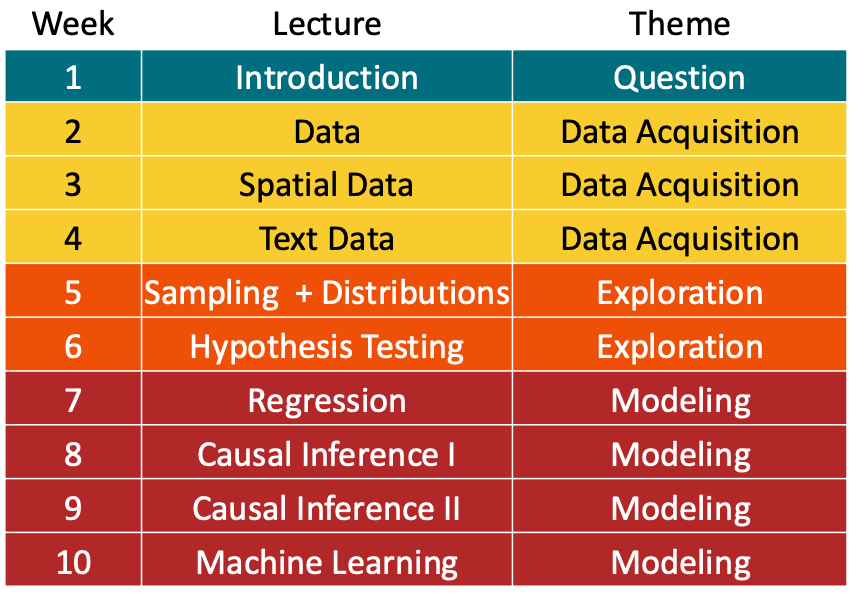
\includegraphics{outline.png}

\bookmarksetup{startatroot}

\hypertarget{python-recap}{%
\chapter{Python Recap}\label{python-recap}}

\hypertarget{workshop-1-open-in-colab}{%
\section[\emph{Workshop 1} ]{\texorpdfstring{\emph{Workshop 1}
\href{https://colab.research.google.com/github/oballinger/QM2/blob/main/notebooks/W01.\%20Python\%20Recap.ipynb}{\protect
\includegraphics{index_files/mediabag/colab-badge.png}}}{Workshop 1 Open In Colab}}\label{workshop-1-open-in-colab}}

\hypertarget{registering-a-github-account}{%
\section{Registering a GitHub
account}\label{registering-a-github-account}}

Before we get started, we need to set a few things up. GitHub is a
platform for software development and version control using Git,
allowing developers to store and manage their code. Think of it as
google docs but for code-- it will be very useful for collaborating on
your group projects later in the term, and in your future as a data
analyst.

\begin{enumerate}
\def\labelenumi{\arabic{enumi}.}
\tightlist
\item
  Use \href{https://github.com/join}{this link} to register for a GitHub
  account if you don't already have one.
\item
  Once that's done, \href{https://github.com/new}{create a new github
  repository} called ``QM2''.
\item
  In this notebook, click ``File'' and then ``Save a copy in GitHub''.
\end{enumerate}

Voila! You now have a version of this notebook saved to your own GitHub
account. \emph{You will need to do step 3 for all the workshops!} Now,
on to python.

\hypertarget{using-python}{%
\section{Using Python}\label{using-python}}

In this course, we'll make extensive use of \emph{Python}, a programming
language used widely in scientific computing and on the web. We will be
using Python as a way to manipulate, plot and analyse data. This isn't a
course about learning Python, it's about working with data - but we'll
learning a little bit of programming along the way.

By now, you should have done the prerequisites for the module, and
understand a bit about how Python is structured, what different commands
do, and so on - this is a bit of a refresher to remind you of what we
need at the beginning of term.

The particular flavour of Python we're using is \emph{iPython}, which,
as we've seen, allows us to combine text, code, images, equations and
figures in a \emph{Notebook}. This is a \emph{cell}, written in
\emph{markdown} - a way of writing nice text. Contrast this with
\emph{code} cell, which executes a bit of Python:

\begin{Shaded}
\begin{Highlighting}[]
\BuiltInTok{print}\NormalTok{(}\DecValTok{2}\OperatorTok{+}\DecValTok{2}\NormalTok{)}
\end{Highlighting}
\end{Shaded}

\begin{verbatim}
4
\end{verbatim}

The Notebook format allows you to engage in what Don Knuth describes as
\href{http://en.wikipedia.org/wiki/Literate_programming}{Literate
Programming}:

\begin{quote}
{[}\ldots{]} Instead of writing code containing documentation, the
literate programmer writes documentation containing code. No longer does
the English commentary injected into a program have to be hidden in
comment delimiters at the top of the file, or under procedure headings,
or at the end of lines. Instead, it is wrenched into the daylight and
made the main focus. The ``program'' then becomes primarily a document
directed at humans, with the code being herded between ``code
delimiters'' from where it can be extracted and shuffled out sideways to
the language system by literate programming tools.
\href{http://www.literateprogramming.com/lpquotes.html}{Ross Williams}
\end{quote}

\hypertarget{libraries}{%
\section{Libraries}\label{libraries}}

We will work with a number of \emph{libraries}, which provide additional
functions and techniques to help us to carry out our tasks.

These include:

\emph{Pandas:} we'll use this a lot to slice and dice data

\emph{matplotlib}: this is our basic graphing software, and we'll also
use it for mapping

\emph{nltk}: The Natural Language Tool Kit will help us work with text

We aren't doing all this to learn to program. We could spend a whole
term learning how to use Python and never look at any data, maps,
graphs, or visualisations. But we do need to understand a few basics to
use Python for working with data. So let's revisit a few concepts that
you should have covered in your prerequisites.

\hypertarget{variables}{%
\section{Variables}\label{variables}}

Python can broadly be divided in verbs and nouns: things which \emph{do}
things, and things which \emph{are} things. In Python, the verbs can be
\emph{commands}, \emph{functions}, or \emph{methods}. We won't worry too
much about the distinction here - suffice it to say, they are the parts
of code which manipulate data, calculate values, or show things on the
screen.

The simplest proper noun object in Python is the \emph{variable}.
Variables are given names and store information. This can be, for
example, numeric, text, or boolean (true/false). These are all
statements setting up variables:

n = 1

t = ``hi''

b = True

Now let's try this in code:

\begin{Shaded}
\begin{Highlighting}[]
\NormalTok{n }\OperatorTok{=} \DecValTok{1}

\NormalTok{t }\OperatorTok{=} \StringTok{"hi"}

\NormalTok{b }\OperatorTok{=} \VariableTok{True}
\end{Highlighting}
\end{Shaded}

Note that each command is on a new line; other than that, the
\emph{syntax} of Python should be fairly clear. We're setting these
variables equal to the letters and numbers and phrases and booleans.
\textbf{What's a boolean?}

The value of this is we now have values tied to these variables - so
every time we want to use it, we can refer to the variable:

\begin{Shaded}
\begin{Highlighting}[]
\NormalTok{n}
\end{Highlighting}
\end{Shaded}

\begin{verbatim}
1
\end{verbatim}

\begin{Shaded}
\begin{Highlighting}[]
\NormalTok{t}
\end{Highlighting}
\end{Shaded}

\begin{verbatim}
'hi'
\end{verbatim}

\begin{Shaded}
\begin{Highlighting}[]
\NormalTok{b}
\end{Highlighting}
\end{Shaded}

\begin{verbatim}
True
\end{verbatim}

Because we've defined these variables in the early part of the notebook,
we can use them later on.

\emph{\textbf{Advanced}: where do \textbf{classes} fit into this
noun/verb picture of variables and commands?}

\hypertarget{where-is-my-data}{%
\section{Where is my data?}\label{where-is-my-data}}

When we work in excel and text editors, we're used to seeing the data
onscreen - and if we manipulate the data in some way (averaging or
summing up), we see both the inputs and outputs on screen. The big
difference in working with Python is that we don't see our variables all
of the time, or the effect we're having on them. They're there in the
background, but it's usually worth checking in on them from time to
time, to see whether our processes are doing what we think they're
doing.

This is pretty easy to do - we can just type the variable name, or
``print(\emph{variable name})'':

\begin{Shaded}
\begin{Highlighting}[]
\NormalTok{n }\OperatorTok{=}\NormalTok{ n}\OperatorTok{+}\DecValTok{1}
\BuiltInTok{print}\NormalTok{(n)}
\BuiltInTok{print}\NormalTok{(t)}
\BuiltInTok{print}\NormalTok{(b)}
\end{Highlighting}
\end{Shaded}

\begin{verbatim}
2
hi
True
\end{verbatim}

\hypertarget{flow}{%
\section{Flow}\label{flow}}

Python, in common with all programming languages, executes commands in a
sequence - we might refer to this as the ``ineluctable march of the
machines'', but it's more common referred to as the \emph{flow} of the
code (we'll use the word ``code'' a lot - it just means commands written
in the programming language). In most cases, code just executes in the
order it's written. This is true within each \emph{cell} (each block of
text in the notebook), and it's true when we execute the cells in order;
that's why we can refer back to the variables we defined earlier:

\begin{Shaded}
\begin{Highlighting}[]
\BuiltInTok{print}\NormalTok{(n)}
\end{Highlighting}
\end{Shaded}

\begin{verbatim}
2
\end{verbatim}

If we make a change to one of these variables, say n:

\begin{Shaded}
\begin{Highlighting}[]
\NormalTok{n }\OperatorTok{=} \DecValTok{3}
\end{Highlighting}
\end{Shaded}

and execute the above ``print n'' command, you'll see that it has
changed n to 3. So if we go out of order, the obvious flow of the code
is confused. For this reason, try to write your code so it executes in
order, one cell at a time. At least for the moment, this will make it
easier to follow the logic of what you're doing to data.

\emph{Advanced}: what happens to this flow when you write
\emph{functions} to automate common tasks?

\textbf{\emph{Exercise - Setting up variables}}:

\begin{enumerate}
\def\labelenumi{\arabic{enumi}.}
\item
  Create a new cell.
\item
  Create the variables ``name'', and assign your name to it.
\item
  Create a variable ``Python'' and assign a score out of 10 to how much
  you like Python.
\item
  Create a variable ``prior'' and if you've used Python before, assign
  True; otherwise assign False to the variable
\item
  Print these out to the screen
\end{enumerate}

\hypertarget{downloading-data}{%
\section{Downloading Data}\label{downloading-data}}

Lets fetch the data we will be using for this session. There are two
ways in which you can upload data to the Colab notebook. You can use the
following code to upload a CSV or similar data file.

\begin{Shaded}
\begin{Highlighting}[]
\ImportTok{from}\NormalTok{ google.colab }\ImportTok{import}\NormalTok{ files}
\NormalTok{uploaded }\OperatorTok{=}\NormalTok{ files.upload()}
\end{Highlighting}
\end{Shaded}

Or you can use the following cell to fetch the data directly from the
QM2 server.

Let's create a folder that we can store all our data for this session

\begin{Shaded}
\begin{Highlighting}[]
\OperatorTok{!}\NormalTok{mkdir data}
\end{Highlighting}
\end{Shaded}

\begin{Shaded}
\begin{Highlighting}[]
\OperatorTok{!}\NormalTok{mkdir .}\OperatorTok{/}\NormalTok{data}\OperatorTok{/}\NormalTok{wk1}
\OperatorTok{!}\NormalTok{curl https:}\OperatorTok{//}\NormalTok{s3.eu}\OperatorTok{{-}}\NormalTok{west}\OperatorTok{{-}}\FloatTok{2.}\ErrorTok{amazonaws}\NormalTok{.com}\OperatorTok{/}\NormalTok{qm2}\OperatorTok{/}\NormalTok{wk1}\OperatorTok{/}\NormalTok{data.csv }\OperatorTok{{-}}\NormalTok{o .}\OperatorTok{/}\NormalTok{data}\OperatorTok{/}\NormalTok{wk1}\OperatorTok{/}\NormalTok{data.csv}
\OperatorTok{!}\NormalTok{curl https:}\OperatorTok{//}\NormalTok{s3.eu}\OperatorTok{{-}}\NormalTok{west}\OperatorTok{{-}}\FloatTok{2.}\ErrorTok{amazonaws}\NormalTok{.com}\OperatorTok{/}\NormalTok{qm2}\OperatorTok{/}\NormalTok{wk1}\OperatorTok{/}\NormalTok{sample\_group.csv }\OperatorTok{{-}}\NormalTok{o .}\OperatorTok{/}\NormalTok{data}\OperatorTok{/}\NormalTok{wk1}\OperatorTok{/}\NormalTok{sample\_group.csv}
\end{Highlighting}
\end{Shaded}

\begin{verbatim}
  % Total    % Received % Xferd  Average Speed   Time    Time     Time  Current
                                 Dload  Upload   Total   Spent    Left  Speed
100   203  100   203    0     0   2872      0 --:--:-- --:--:-- --:--:--  3029
  % Total    % Received % Xferd  Average Speed   Time    Time     Time  Current
                                 Dload  Upload   Total   Spent    Left  Speed
100   297  100   297    0     0   1844      0 --:--:-- --:--:-- --:--:--  1879
\end{verbatim}

\hypertarget{storing-and-importing-data}{%
\section{Storing and importing data}\label{storing-and-importing-data}}

Typically, data we look at won't be just one number, or one bit of text.
Python has a lot of different ways of dealing with a bunch of numbers:
for example, a list of values is called a \textbf{list}:

\begin{Shaded}
\begin{Highlighting}[]
\NormalTok{listy }\OperatorTok{=}\NormalTok{ [}\DecValTok{1}\NormalTok{,}\DecValTok{2}\NormalTok{,}\DecValTok{3}\NormalTok{,}\DecValTok{6}\NormalTok{,}\DecValTok{9}\NormalTok{]}
\BuiltInTok{print}\NormalTok{(listy)}
\end{Highlighting}
\end{Shaded}

\begin{verbatim}
[1, 2, 3, 6, 9]
\end{verbatim}

A set of values \emph{linked} to an index (or key) is called a
\textbf{dictionary}; for example:

\begin{Shaded}
\begin{Highlighting}[]
\NormalTok{dicty }\OperatorTok{=}\NormalTok{ \{}\StringTok{\textquotesingle{}Bob\textquotesingle{}}\NormalTok{: }\FloatTok{1.2}\NormalTok{, }\StringTok{\textquotesingle{}Mike\textquotesingle{}}\NormalTok{: }\FloatTok{1.2}\NormalTok{, }\StringTok{\textquotesingle{}Coop\textquotesingle{}}\NormalTok{: }\FloatTok{1.1}\NormalTok{, }\StringTok{\textquotesingle{}Maddy\textquotesingle{}}\NormalTok{: }\FloatTok{1.3}\NormalTok{, }\StringTok{\textquotesingle{}Giant\textquotesingle{}}\NormalTok{: }\FloatTok{2.1}\NormalTok{\}}
\BuiltInTok{print}\NormalTok{(dicty)}
\end{Highlighting}
\end{Shaded}

\begin{verbatim}
{'Bob': 1.2, 'Mike': 1.2, 'Coop': 1.1, 'Maddy': 1.3, 'Giant': 2.1}
\end{verbatim}

Notice that the list uses square brackets with values separated by
commas, and the dict uses curly brackets with pairs separated by commas,
and colons (:) to link a \emph{key} (index or address) with a value.

(You might notice that they haven't printed out in the order you entered
them)

*\textbf{Advanced}: Print out 1) The third element of \textbf{listy},
and 2) The element of \textbf{dicty} relating to Giant

We'll discuss different ways of organising data again soon, but for now
we'll look at \emph{dataframes} - the way our data-friendly
\emph{library} \textbf{Pandas} works with data. We'll be using Pandas a
lot this term, so it's good to get started with it early.

Let's start by importing pandas. We'll also import another library, but
we're not going to worry about that too much at the moment.

If you see a warning about `Building Font Cache' don't worry - this is
normal.

\begin{Shaded}
\begin{Highlighting}[]
\ImportTok{import}\NormalTok{ pandas}

\ImportTok{import}\NormalTok{ matplotlib}
\OperatorTok{\%}\NormalTok{matplotlib inline}
\end{Highlighting}
\end{Shaded}

Let's import a simple dataset and show it in pandas. We'll use a
pre-prepared ``.csv'' file, which needs to be in the same folder as our
code.

\begin{Shaded}
\begin{Highlighting}[]
\NormalTok{data }\OperatorTok{=}\NormalTok{ pandas.read\_csv(}\StringTok{\textquotesingle{}./data/wk1/data.csv\textquotesingle{}}\NormalTok{)}
\NormalTok{data.head()}
\end{Highlighting}
\end{Shaded}

\begin{longtable}[]{@{}llllll@{}}
\toprule\noalign{}
& Name & First Appearance & Approx height & Gender & Law Enforcement \\
\midrule\noalign{}
\endhead
\bottomrule\noalign{}
\endlastfoot
0 & Bob & 1.2 & 6.0 & Male & False \\
1 & Mike & 1.2 & 5.5 & Male & False \\
2 & Coop & 1.1 & 6.0 & Male & True \\
3 & Maddy & 1.3 & 5.5 & Female & False \\
4 & Giant & 2.1 & 7.5 & Male & False \\
\end{longtable}

What we've done here is read in a .csv file into a dataframe, the object
pandas uses to work with data, and one that has lots of methods for
slicing and dicing data, as we will see over the coming weeks. The
head() command tells iPython to show the first few columns/rows of the
data, so we can start to get a sense of what the data looks like and
what sort of type of objects is represents.

A common first step for exploring our data is to sort it. In Pandas,
this can be done easily with the \texttt{sort\_values()} function. We
can specify which column to sort the data by, and whether we want to
sort in ascending or descending order, using the optional arguments
\texttt{by} and \texttt{ascending}, respectively. In the example below,
we're sorting in \emph{descending} order of height:

\begin{Shaded}
\begin{Highlighting}[]
\NormalTok{data.sort\_values(by}\OperatorTok{=}\StringTok{\textquotesingle{}Approx height\textquotesingle{}}\NormalTok{, ascending}\OperatorTok{=}\VariableTok{False}\NormalTok{).head()}
\end{Highlighting}
\end{Shaded}

\begin{longtable}[]{@{}llllll@{}}
\toprule\noalign{}
& Name & First Appearance & Approx height & Gender & Law Enforcement \\
\midrule\noalign{}
\endhead
\bottomrule\noalign{}
\endlastfoot
4 & Giant & 2.1 & 7.5 & Male & False \\
0 & Bob & 1.2 & 6.0 & Male & False \\
2 & Coop & 1.1 & 6.0 & Male & True \\
1 & Mike & 1.2 & 5.5 & Male & False \\
3 & Maddy & 1.3 & 5.5 & Female & False \\
\end{longtable}

\bookmarksetup{startatroot}

\hypertarget{supplementary-kaggle-exercises}{%
\chapter{Supplementary: Kaggle
exercises}\label{supplementary-kaggle-exercises}}

If you've gotten this far, congratulations! To further hone your skills,
try working your way through the five
\href{https://www.kaggle.com/learn/intro-to-programming}{intro to
programming notebooks on Kaggle}. These cover a range of skills that
we'll be using throughout the term. Kaggle is a very useful resource for
learning data science, so making an account may not be a bad idea!

\bookmarksetup{startatroot}

\hypertarget{assessed-question}{%
\chapter{Assessed Question}\label{assessed-question}}

\begin{Shaded}
\begin{Highlighting}[]
\CommentTok{\# use this code cell to answer the question}
\end{Highlighting}
\end{Shaded}

\bookmarksetup{startatroot}

\hypertarget{intro-to-pandas}{%
\chapter{Intro to Pandas}\label{intro-to-pandas}}

\hypertarget{workshop-2-open-in-colab}{%
\section[\emph{Workshop 2} ]{\texorpdfstring{\emph{Workshop 2}
\href{https://colab.research.google.com/github/oballinger/QM2/blob/main/notebooks/W02.\%20Pandas.ipynb}{\protect
\includegraphics{notebooks/../colab-badge.png}}}{Workshop 2 Open In Colab}}\label{workshop-2-open-in-colab}}

In this workshop, our aim is to get used to working with more complex
data that we've imported from external files. We'll start to graph it,
and to slice and dice it, to select the bits we're interested in.

We will work with \emph{pandas} to manipulate the data, and to derive
measures and graphs that tell us a bit more than what the source data
files tell us.

\hypertarget{aims}{%
\subsection{Aims}\label{aims}}

\begin{itemize}
\tightlist
\item
  Learn to import data to python using pandas
\item
  Learn how access specific rows, columns and cells
\item
  Plot the data
\item
  Tidy up graphs to include axes
\end{itemize}

\hypertarget{introduction}{%
\section{Introduction}\label{introduction}}

We are going to work with some UK income data. The income data is
packaged as a .csv file. The Pandas package knows how to handle this and
put the data in a DataFrame, as we've seen. Let's examine the data and
start to see what we can say about it. First of all, we have to find
data - I'm interested in looking in data with a wide spread, so I looked
for data on income in the UK.

This data is collected by the Office for National Statistics(ONS) :
http://www.ons.gov.uk/ons/datasets-and-tables/index.html?pageSize=50\&sortBy=none\&sortDirection=none\&newquery=income+percentile
- but the exact data I want to see, income by percentile, is tricky to
find.

I ended up using data from 2011, generated from a study called the
Family Resources Survey and collated and tweaked by an independent
research unit called the Institute of Fiscal Studies (IFS). The
``tweaking'' they do tends to be around the size of the family unit, and
other factors which create economies of scale - hence they
``equivalise'' it. The IFS is quoted in UK Government documents, so we
can have some trust in their impartiality, or at least accuracy - of
course, if we were publishing research about this, that's not really
good enough and we'd want to reproduce, or at least understand and
critique, their methodology rather than just trusting it!

e.g.:

http://www.ifs.org.uk/wheredoyoufitin/about.php

https://en.wikipedia.org/wiki/Equivalisation

\hypertarget{downloading-the-data}{%
\section{Downloading the Data}\label{downloading-the-data}}

Let's grab our income data from our course website and save it into our
data folder. If you've not already created a data folder then do so
using the following command. Don't worry if it generates an error, that
means you've already got a data folder.

\begin{Shaded}
\begin{Highlighting}[]
\OperatorTok{!}\NormalTok{mkdir data}
\end{Highlighting}
\end{Shaded}

\begin{verbatim}
mkdir: data: File exists
\end{verbatim}

\begin{Shaded}
\begin{Highlighting}[]
\OperatorTok{!}\NormalTok{mkdir data}\OperatorTok{/}\NormalTok{wk2}
\OperatorTok{!}\NormalTok{curl https:}\OperatorTok{//}\NormalTok{s3.eu}\OperatorTok{{-}}\NormalTok{west}\OperatorTok{{-}}\FloatTok{2.}\ErrorTok{amazonaws}\NormalTok{.com}\OperatorTok{/}\NormalTok{qm2}\OperatorTok{/}\NormalTok{wk2}\OperatorTok{/}\NormalTok{incomes.csv }\OperatorTok{{-}}\NormalTok{o .}\OperatorTok{/}\NormalTok{data}\OperatorTok{/}\NormalTok{wk2}\OperatorTok{/}\NormalTok{incomes.csv}
\end{Highlighting}
\end{Shaded}

\begin{verbatim}
mkdir: data/wk2: File exists
  % Total    % Received % Xferd  Average Speed   Time    Time     Time  Current
                                 Dload  Upload   Total   Spent    Left  Speed
100 15154  100 15154    0     0   135k      0 --:--:-- --:--:-- --:--:--  143k
\end{verbatim}

\begin{Shaded}
\begin{Highlighting}[]
\ImportTok{import}\NormalTok{ pandas}
\ImportTok{import}\NormalTok{ pylab}
\ImportTok{import}\NormalTok{ matplotlib.pyplot }\ImportTok{as}\NormalTok{ plt}
\CommentTok{\# make the plots a little wider by default}
\OperatorTok{\%}\NormalTok{matplotlib inline}
\NormalTok{plt.style.use(}\StringTok{\textquotesingle{}ggplot\textquotesingle{}}\NormalTok{)}

\NormalTok{pylab.rcParams[}\StringTok{\textquotesingle{}figure.figsize\textquotesingle{}}\NormalTok{] }\OperatorTok{=}\NormalTok{ (}\FloatTok{10.}\NormalTok{, }\FloatTok{8.}\NormalTok{)}
\end{Highlighting}
\end{Shaded}

\begin{Shaded}
\begin{Highlighting}[]
\NormalTok{data\_path }\OperatorTok{=} \StringTok{"./data/wk2/incomes.csv"}

\NormalTok{income }\OperatorTok{=}\NormalTok{  pandas.read\_csv(data\_path, index\_col}\OperatorTok{=}\DecValTok{0}\NormalTok{)}
\NormalTok{income.head()}
\end{Highlighting}
\end{Shaded}

\begin{longtable}[]{@{}llllllllllllllll@{}}
\toprule\noalign{}
& Net equivalised household income in 2010-11, week & Childless couple,
annual income & Couple, two children under 14 & Couple, three children
under 14 & Couple with one child under 14 & Couple with two children
aged 15 to 18 & Couple, two children under 14 plus dependent adult &
Single adult & Lone parent, one child under 14 & Lone parent, two
children under 14 & Lone parent, two children aged 15-18 & ANNOTATIONS &
1979 to 1996-97 & 1996-97 to 2009-10 & 1996-97 to 2010-11 \\
Percentile Point & & & & & & & & & & & & & & & \\
\midrule\noalign{}
\endhead
\bottomrule\noalign{}
\endlastfoot
1 & 33.50 & 1,746.92 & 2,445.69 & 2,795.08 & 2,096.31 & 2,899.89 &
3,022.18 & 1,170.44 & 1,519.82 & 1,869.21 & 2,323.41 & NaN & NaN & NaN &
NaN \\
2 & 98.60 & 5,141.01 & 7,197.41 & 8,225.61 & 6,169.21 & 8,534.07 &
8,893.95 & 3,444.48 & 4,472.68 & 5,500.88 & 6,837.54 & NaN & -0.20\% &
-1.30\% & -0.50\% \\
3 & 128.56 & 6,703.11 & 9,384.36 & 10,724.98 & 8,043.74 & 11,127.17 &
11,596.39 & 4,491.09 & 5,831.71 & 7,172.33 & 8,915.14 & NaN & 0.40\% &
0.10\% & 0.10\% \\
4 & 151.05 & 7,875.75 & 11,026.05 & 12,601.20 & 9,450.90 & 13,073.75 &
13,625.05 & 5,276.75 & 6,851.90 & 8,427.05 & 10,474.75 & NaN & 0.50\% &
0.80\% & 0.60\% \\
5 & 166.32 & 8,671.91 & 12,140.68 & 13,875.06 & 10,406.30 & 14,395.38 &
15,002.41 & 5,810.18 & 7,544.57 & 9,278.95 & 11,533.65 & NaN & 0.70\% &
1.00\% & 0.90\% \\
\end{longtable}

This is a simple dataframe - we see the percentile and an income. Note
that I've told pandas to use the first column (the Percentile) as the
index to make life easier.

The percentile tells us how people on that income rank - so the final
category, 99\% (which is really binned, so 99\%\textless n\(\leq\)
100\%), is telling us how much ``the 1\%'' earn. Let's find out:

\begin{Shaded}
\begin{Highlighting}[]
\NormalTok{income.tail()}
\end{Highlighting}
\end{Shaded}

\begin{longtable}[]{@{}llllllllllllllll@{}}
\toprule\noalign{}
& Net equivalised household income in 2010-11, week & Childless couple,
annual income & Couple, two children under 14 & Couple, three children
under 14 & Couple with one child under 14 & Couple with two children
aged 15 to 18 & Couple, two children under 14 plus dependent adult &
Single adult & Lone parent, one child under 14 & Lone parent, two
children under 14 & Lone parent, two children aged 15-18 & ANNOTATIONS &
1979 to 1996-97 & 1996-97 to 2009-10 & 1996-97 to 2010-11 \\
Percentile Point & & & & & & & & & & & & & & & \\
\midrule\noalign{}
\endhead
\bottomrule\noalign{}
\endlastfoot
95 & 1075.73 & 56,088.56 & 78,523.99 & 89,741.70 & 67,306.27 & 93,107.01
& 97,033.21 & 37,579.34 & 48,797.05 & 60,014.76 & 74,597.79 & NaN &
2.90\% & 2.00\% & 1.30\% \\
96 & 1174.48 & 61,237.18 & 85,732.05 & 97,979.49 & 73,484.61 &
101,653.72 & 105,940.32 & 41,028.91 & 53,276.35 & 65,523.78 & 81,445.45
& NaN & 3.00\% & 2.00\% & 1.40\% \\
97 & 1302.74 & 67,925.07 & 95,095.10 & 108,680.12 & 81,510.09 &
112,755.62 & 117,510.37 & 45,509.80 & 59,094.81 & 72,679.83 & 90,340.35
& NaN & 3.20\% & 2.20\% & 1.60\% \\
98 & 1523.31 & 79,425.23 & 111,195.32 & 127,080.36 & 95,310.27 &
131,845.88 & 137,405.64 & 53,214.90 & 69,099.95 & 84,984.99 & 105,635.55
& NaN & 3.20\% & 2.70\% & 1.70\% \\
99 & 2090.35 & 108,990.74 & 152,587.04 & 174,385.19 & 130,788.89 &
180,924.64 & 188,553.99 & 73,023.80 & 94,821.95 & 116,620.10 &
144,957.69 & NaN & NaN & NaN & NaN \\
\end{longtable}

Well, they we have it - the 1\% earn, on average, about £2000 a week.
How does that compare to people in the 90\% decile? We can access
particular \emph{rows} in a dataframe using \textbf{.loc{[}row
index{]}}; because our index is the percentile point, we can just read
it off:

\begin{Shaded}
\begin{Highlighting}[]
\NormalTok{income.loc[}\DecValTok{90}\NormalTok{]}
\end{Highlighting}
\end{Shaded}

\begin{verbatim}
Net equivalised household income in 2010-11, week        845.54
Childless couple, annual income                       44,086.54
Couple, two children under 14                         61,721.15
Couple, three children under 14                       70,538.46
Couple with one child under 14                        52,903.85
Couple with two children aged 15 to 18                73,183.65
Couple, two children under 14 plus dependent adult    76,269.71
Single adult                                          29,537.98
Lone parent, one child under 14                       38,355.29
Lone parent, two children under 14                    47,172.60
Lone parent, two children aged 15-18                  58,635.10
ANNOTATIONS                                                 NaN
1979 to 1996-97                                           2.50%
1996-97 to 2009-10                                        1.70%
1996-97 to 2010-11                                        1.20%
Name: 90, dtype: object
\end{verbatim}

We can also select a range of values with the ``colon'' notation. This
will select the 90-95th percentiles, for example:

\begin{Shaded}
\begin{Highlighting}[]
\NormalTok{income.loc[}\DecValTok{90}\NormalTok{:}\DecValTok{95}\NormalTok{]}
\end{Highlighting}
\end{Shaded}

\begin{longtable}[]{@{}llllllllllllllll@{}}
\toprule\noalign{}
& Net equivalised household income in 2010-11, week & Childless couple,
annual income & Couple, two children under 14 & Couple, three children
under 14 & Couple with one child under 14 & Couple with two children
aged 15 to 18 & Couple, two children under 14 plus dependent adult &
Single adult & Lone parent, one child under 14 & Lone parent, two
children under 14 & Lone parent, two children aged 15-18 & ANNOTATIONS &
1979 to 1996-97 & 1996-97 to 2009-10 & 1996-97 to 2010-11 \\
Percentile Point & & & & & & & & & & & & & & & \\
\midrule\noalign{}
\endhead
\bottomrule\noalign{}
\endlastfoot
90 & 845.54 & 44,086.54 & 61,721.15 & 70,538.46 & 52,903.85 & 73,183.65
& 76,269.71 & 29,537.98 & 38,355.29 & 47,172.60 & 58,635.10 & NaN &
2.50\% & 1.70\% & 1.20\% \\
91 & 876.63 & 45,707.74 & 63,990.84 & 73,132.39 & 54,849.29 & 75,874.85
& 79,074.40 & 30,624.19 & 39,765.74 & 48,907.29 & 60,791.30 & NaN &
2.60\% & 1.70\% & 1.20\% \\
92 & 911.29 & 47,514.54 & 66,520.35 & 76,023.26 & 57,017.44 & 78,874.13
& 82,200.15 & 31,834.74 & 41,337.65 & 50,840.55 & 63,194.33 & NaN &
2.60\% & 1.80\% & 1.20\% \\
93 & 957.14 & 49,905.23 & 69,867.32 & 79,848.36 & 59,886.27 & 82,842.68
& 86,336.04 & 33,436.50 & 43,417.55 & 53,398.59 & 66,373.95 & NaN &
2.70\% & 1.80\% & 1.30\% \\
94 & 1016.37 & 52,993.38 & 74,190.73 & 84,789.40 & 63,592.05 & 87,969.00
& 91,678.54 & 35,505.56 & 46,104.24 & 56,702.91 & 70,481.19 & NaN &
2.90\% & 1.90\% & 1.30\% \\
95 & 1075.73 & 56,088.56 & 78,523.99 & 89,741.70 & 67,306.27 & 93,107.01
& 97,033.21 & 37,579.34 & 48,797.05 & 60,014.76 & 74,597.79 & NaN &
2.90\% & 2.00\% & 1.30\% \\
\end{longtable}

\hypertarget{accessing-parts-of-a-dataframe}{%
\section{Accessing parts of a
dataframe}\label{accessing-parts-of-a-dataframe}}

If we want to extract the actual value instead of just the whole row, we
need to reference the \emph{column} as well as the row. In pandas,
columns are referenced by \textbf{column name}:

\begin{Shaded}
\begin{Highlighting}[]
\NormalTok{income[}\StringTok{\textquotesingle{}Net equivalised household income in 2010{-}11, week\textquotesingle{}}\NormalTok{]}
\end{Highlighting}
\end{Shaded}

\begin{verbatim}
Percentile Point
1       33.50
2       98.60
3      128.56
4      151.05
5      166.32
       ...   
95    1075.73
96    1174.48
97    1302.74
98    1523.31
99    2090.35
Name: Net equivalised household income in 2010-11, week, Length: 99, dtype: float64
\end{verbatim}

So, to access a particular cell, we tell Python the row and the column
(this is pretty simple - the same way we tell excel to access cell
``A34'' meaning Column A, Row 34). One way we do that in pandas is to
select the column, and then use .loc{[}{]} on the index.

\begin{Shaded}
\begin{Highlighting}[]
\NormalTok{income[}\StringTok{\textquotesingle{}Net equivalised household income in 2010{-}11, week\textquotesingle{}}\NormalTok{].loc[}\DecValTok{90}\NormalTok{]}
\end{Highlighting}
\end{Shaded}

\begin{verbatim}
845.54
\end{verbatim}

We've accessed row 90 of the column called `Net equivalised household
income in 2010-11, week'; can we access the data the other way around -
can we first take the row and then specify a column? Let's try:

\begin{Shaded}
\begin{Highlighting}[]
\NormalTok{income.loc[}\DecValTok{90}\NormalTok{][}\StringTok{\textquotesingle{}Net equivalised household income in 2010{-}11, week\textquotesingle{}}\NormalTok{]}
\end{Highlighting}
\end{Shaded}

\begin{verbatim}
845.54
\end{verbatim}

Yes, this seems to be working fine.

\hypertarget{extension}{%
\subsection{Extension}\label{extension}}

The reason for this is that selecting the column spits out a smaller
dataframe, and all dataframes use ``loc'', so we can use that. Another
way to do this would be to use an explicit variable for the dataframe,
along the lines of:

\texttt{smallDataFrame\ =\ income{[}\textquotesingle{}Net\ equivalised\ household\ income\ in\ 2010-11,\ week\textquotesingle{}{]}}\strut \\
\texttt{smallDataFrame.loc{[}90{]}}

by doing income

\texttt{{[}\textquotesingle{}Net\ equivalised\ household\ income\ in\ 2010-11,\ week\textquotesingle{}{]}.loc{[}90{]}}

we're taking the ``smallDataFrame'' object as an implicit (or hidden)
output

If we want to look at a few rows of data, we can use a range:

\begin{Shaded}
\begin{Highlighting}[]
\NormalTok{income[}\StringTok{\textquotesingle{}Net equivalised household income in 2010{-}11, week\textquotesingle{}}\NormalTok{].loc[}\DecValTok{90}\NormalTok{:}\DecValTok{95}\NormalTok{]}
\end{Highlighting}
\end{Shaded}

\begin{verbatim}
Percentile Point
90     845.54
91     876.63
92     911.29
93     957.14
94    1016.37
95    1075.73
Name: Net equivalised household income in 2010-11, week, dtype: float64
\end{verbatim}

So, to recap, we can now access a particular \textbf{row} using
\emph{loc{[}index number{]}}, a particular \textbf{column} with the
square brackets formalism \emph{dataframename{[}`column name'{]}}, or
both \emph{dataframename{[}`column name'{]}.loc{[}index number{]}}.
We've made a start at being able to get to the bits of data we need.

\hypertarget{exercise}{%
\section{Exercise:}\label{exercise}}

How do the equivalised incomes of single adults and childless couples
compare? Look at the 1st, 99th and 50th percentile and summarise what
this tells you about the value or price of coupling.

\hypertarget{examining-the-distribution}{%
\section{Examining the Distribution}\label{examining-the-distribution}}

Returning to the overall statistics, the 90\% percentile earns less than
half the top percentile (``the 1\%''); if you're taking home over £800
as a household, you're in the top 10\% of earners.

How does 1. The income of ``the 1\%'' compare with the mean and median
across the population, as a proportion? 2. How does the 1\% compare with
the 90th percentile (the 10\%)? 3. How does the 10\% compare with the
median and mean?

The 1\% earn about 60 times the poorest groups in society - and we've
made other comparisons. But that's not the whole story. Let's look at
the income graph.

In pandas, we can plot this fairly easily\ldots{}

\begin{Shaded}
\begin{Highlighting}[]
\NormalTok{income[}\StringTok{\textquotesingle{}Net equivalised household income in 2010{-}11, week\textquotesingle{}}\NormalTok{].plot()}
\NormalTok{plt.title(}\StringTok{\textquotesingle{}UK Net Equivalised Income by Percentile per week, 2010{-}11\textquotesingle{}}\NormalTok{)}
\NormalTok{plt.xlabel(}\StringTok{\textquotesingle{}Income Percentile\textquotesingle{}}\NormalTok{)}
\NormalTok{plt.ylabel(}\StringTok{\textquotesingle{}Income (Net, Equivalised) [GBP]\textquotesingle{}}\NormalTok{)}
\end{Highlighting}
\end{Shaded}

\begin{verbatim}
Text(0, 0.5, 'Income (Net, Equivalised) [GBP]')
\end{verbatim}

\begin{figure}[H]

{\centering \includegraphics{notebooks/W02. Pandas_files/figure-pdf/cell-13-output-2.png}

}

\end{figure}

We see a curve that is pretty linear in the middle region, but curves
rapidly upwards in the higher percentile and looks more like a power
law.

\hypertarget{exercise-means}{%
\subsection{Exercise: Means}\label{exercise-means}}

Where does the mean appear here? Draw in a horizontal line to show the
mean using \textbf{axhline}. Show the median on the same graph. What is
the meaning of the median in this context?

Hint: Recall that last time we used \emph{axvline} to highlight the mean
and standard deviation by drawing vertical lines on the axis. Here, we
use \emph{axhline} to draw horizontal lines.

\hypertarget{extension-accessing-cells}{%
\subsection{Extension: Accessing
cells}\label{extension-accessing-cells}}

There are a number of ways to access elements of the dataframe: we've
shown how to access columns by the {[}\emph{`name of column'}{]} method,
and rows via the .loc{[}\emph{index}{]} method; and how we can select a
range. There are also .iloc methods to select by number rather than
name; you should become familiar with these on the documentation page
for pandas.

\hypertarget{comparing-segments}{%
\section{Comparing segments}\label{comparing-segments}}

Earlier, we compared some summary statistics of single people and
couples. Let's look at the wider curve for more than one group, now:

\begin{Shaded}
\begin{Highlighting}[]
\CommentTok{\#This is going to throw a load of errors}
\NormalTok{income[[}\StringTok{\textquotesingle{}Single adult\textquotesingle{}}\NormalTok{,}\StringTok{\textquotesingle{}Lone parent, one child under 14\textquotesingle{}}\NormalTok{]].plot()}
\end{Highlighting}
\end{Shaded}

\begin{verbatim}
TypeError: no numeric data to plot
\end{verbatim}

\hypertarget{warning}{%
\section{Warning}\label{warning}}

This isn't looking good. There's a load of text and no graph. If you've
not seen this before, it's an error - something has gone wrong.
Generally, if we look at the \textbf{final} line, it should tell us
what's wrong, in this case there's ``no numeric data to plot'', which is
weird, because we've seen the data and have even plotted some of it.

\hypertarget{messy-data}{%
\section{Messy Data}\label{messy-data}}

DataFrames, as we are starting to see, give us the chance to plot, chop,
slice and data to help us make sense of it. Here, we will create a
\textbf{new} DataFrame to take only two columns of data, and get rid of
any blank cells and any cells which are not being read as numbers -
normally a sign of a missing value or a non-numerical character. Why
could this be happening? It could be

\begin{itemize}
\item
  due to blank spaces in the text file
\item
  due to letters where there should be numbers
\item
  due to characters (``,'', ``-'', etc) that shouldn't really be there
\end{itemize}

In general, there will be some detective work required to figure out
what's wrong in our text file. Your best bet is sometimes to open up the
data in a text editor, like I've done here:

\begin{Shaded}
\begin{Highlighting}[]
\ImportTok{from}\NormalTok{ IPython.display }\ImportTok{import}\NormalTok{ Image}

\NormalTok{data\_path }\OperatorTok{=} \StringTok{"https://s3.eu{-}west{-}2.amazonaws.com/qm2/wk2/data.png"}
\NormalTok{Image(data\_path)}
\end{Highlighting}
\end{Shaded}

\begin{figure}[H]

{\centering \includegraphics{notebooks/W02. Pandas_files/figure-pdf/cell-15-output-1.png}

}

\end{figure}

That's a screenshot of our datafile, opened up in a text editor. As we
can see, these numbers are separated by commas and surrounded by
quotation marks - this is normal, and what .csv files are supposed to
look like. However, there are a lot of commas within the numbers - which
makes it easier for people to read, but confuses software. Luckily,
Python has a method for dealing with this - the ``replace'' method.

Unfortunately, this dataframe is quite messy, so I'm going to have to
extract just the columns of data I'm interested in to make it work. I'll
do that by creating a new dataframe:

\hypertarget{example-cleaning-data}{%
\section{Example: Cleaning data}\label{example-cleaning-data}}

\begin{Shaded}
\begin{Highlighting}[]
\NormalTok{clean }\OperatorTok{=}\NormalTok{ income[[}\StringTok{\textquotesingle{}Childless couple, annual income\textquotesingle{}}\NormalTok{,}\StringTok{\textquotesingle{}Couple, two children under 14\textquotesingle{}}\NormalTok{]]}
\NormalTok{clean.head()}
\end{Highlighting}
\end{Shaded}

\begin{longtable}[]{@{}lll@{}}
\toprule\noalign{}
& Childless couple, annual income & Couple, two children under 14 \\
Percentile Point & & \\
\midrule\noalign{}
\endhead
\bottomrule\noalign{}
\endlastfoot
1 & 1,746.92 & 2,445.69 \\
2 & 5,141.01 & 7,197.41 \\
3 & 6,703.11 & 9,384.36 \\
4 & 7,875.75 & 11,026.05 \\
5 & 8,671.91 & 12,140.68 \\
\end{longtable}

We see those pesky commas. Now we can get on with cleaning up the data:

\begin{Shaded}
\begin{Highlighting}[]
\NormalTok{clean}\OperatorTok{=}\NormalTok{clean.replace(}\StringTok{\textquotesingle{},\textquotesingle{}}\NormalTok{, }\StringTok{\textquotesingle{}\textquotesingle{}}\NormalTok{, regex}\OperatorTok{=}\VariableTok{True}\NormalTok{)}

\CommentTok{\# In addition, missing values are sometimes written as \textquotesingle{}{-}\textquotesingle{}, in order for Python to understand that it is just a missing numerical }
\CommentTok{\# value, all \textquotesingle{}{-}\textquotesingle{} need to be replaced with \textquotesingle{}NaN\textquotesingle{}.}
\NormalTok{clean }\OperatorTok{=}\NormalTok{ clean.replace(}\StringTok{\textquotesingle{}{-}\textquotesingle{}}\NormalTok{, }\StringTok{\textquotesingle{}NaN\textquotesingle{}}\NormalTok{, regex}\OperatorTok{=}\VariableTok{True}\NormalTok{).astype(}\StringTok{\textquotesingle{}float\textquotesingle{}}\NormalTok{)}
\NormalTok{clean.head()}
\end{Highlighting}
\end{Shaded}

\begin{longtable}[]{@{}lll@{}}
\toprule\noalign{}
& Childless couple, annual income & Couple, two children under 14 \\
Percentile Point & & \\
\midrule\noalign{}
\endhead
\bottomrule\noalign{}
\endlastfoot
1 & 1746.92 & 2445.69 \\
2 & 5141.01 & 7197.41 \\
3 & 6703.11 & 9384.36 \\
4 & 7875.75 & 11026.05 \\
5 & 8671.91 & 12140.68 \\
\end{longtable}

\textbf{Extension}: ``\textbf{Regex}'' refers to ``\textbf{Reg}ular
\textbf{Ex}pression'', which is a way of replacing and cleaning text.
It's a bit beyond the scope of this class, but worth looking into if
you're interested in programming more widely.

This seems to have done the job. We've also put a line in the code to
get rid of dashes - a way that data collectors will sometimes represent
missing data. Now let's plot this.

\hypertarget{asking-more-questions-of-the-data}{%
\section{Asking more questions of the
data}\label{asking-more-questions-of-the-data}}

For me, this data starts to beg further questions. How would we answer
these?

\begin{itemize}
\item
  If the top 20\% of income shows such a sharp increase, how do we know
  that there isn't a similar uptick \emph{within} the 1\%? We've already
  seen that the mean of the dataset as a whole is much less than the
  half the maximum category (it's 25\% of the maximum). What if that's
  true within the 1\%, and £2,000/week as a fraction of the 0.1\%, or
  the 0.01\%?
\item
  How does this break down for gender, or educational background, or
  other factors like ethnicity or country of origin?
\item
  Which parts of the income curve show greater gaps between these
  subgroups and what might it say about the underlying causal
  mechanisms?
\end{itemize}

\begin{Shaded}
\begin{Highlighting}[]
\NormalTok{clean.plot()}
\NormalTok{plt.title(}\StringTok{\textquotesingle{}A Modest Proposal: The fiscal benefits of childbirth\textquotesingle{}}\NormalTok{)}
\NormalTok{plt.xlabel(}\StringTok{\textquotesingle{}Percentile\textquotesingle{}}\NormalTok{)}
\NormalTok{plt.ylabel(}\StringTok{\textquotesingle{}Income Per Week [GBP]\textquotesingle{}}\NormalTok{)}
\end{Highlighting}
\end{Shaded}

\begin{verbatim}
Text(0, 0.5, 'Income Per Week [GBP]')
\end{verbatim}

\begin{figure}[H]

{\centering 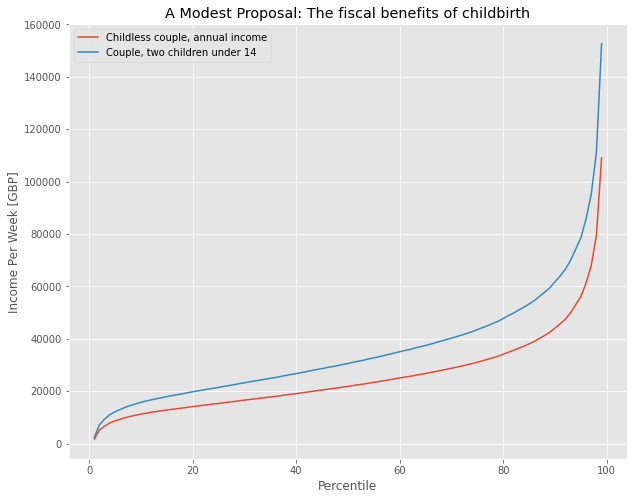
\includegraphics{notebooks/W02. Pandas_files/figure-pdf/cell-18-output-2.png}

}

\end{figure}

\hypertarget{exercise-1}{%
\section{Exercise:}\label{exercise-1}}

Previously, we'd examined income gaps between single people and couples
(how very romantic). Repeat the above exercise (cleaning and plotting
income data) for the columns we used above for single people and
childless couples. Reflect and comment on the differences.

\begin{Shaded}
\begin{Highlighting}[]
\BuiltInTok{print}\NormalTok{(}\StringTok{"Enter your code here"}\NormalTok{)}
\end{Highlighting}
\end{Shaded}

\begin{Shaded}
\begin{Highlighting}[]
\NormalTok{Add your reflection here.}
\end{Highlighting}
\end{Shaded}

So far, we've dealt with selecting data in a particular row of column by
index or label. What if we now want to filter the data by \emph{value}?
For example, let's say I want to see the data for all Childless couples
who earn more than 50,000 (net equivalised) pounds every year. This
looks like:

\begin{Shaded}
\begin{Highlighting}[]
\NormalTok{clean }\OperatorTok{=}\NormalTok{ income[[}\StringTok{\textquotesingle{}Childless couple, annual income\textquotesingle{}}\NormalTok{,}\StringTok{\textquotesingle{}Couple, two children under 14\textquotesingle{}}\NormalTok{]]}
\NormalTok{clean }\OperatorTok{=}\NormalTok{ clean.replace(}\StringTok{\textquotesingle{},\textquotesingle{}}\NormalTok{, }\StringTok{\textquotesingle{}\textquotesingle{}}\NormalTok{, regex}\OperatorTok{=}\VariableTok{True}\NormalTok{)}
\NormalTok{clean }\OperatorTok{=}\NormalTok{ clean.replace(}\StringTok{\textquotesingle{}{-}\textquotesingle{}}\NormalTok{, }\StringTok{\textquotesingle{}NaN\textquotesingle{}}\NormalTok{, regex}\OperatorTok{=}\VariableTok{True}\NormalTok{).astype(}\StringTok{\textquotesingle{}float\textquotesingle{}}\NormalTok{)}
\NormalTok{clean[clean[}\StringTok{\textquotesingle{}Childless couple, annual income\textquotesingle{}}\NormalTok{]}\OperatorTok{\textgreater{}}\DecValTok{50000}\NormalTok{]}
\end{Highlighting}
\end{Shaded}

The key line of code for selection is:

\begin{Shaded}
\begin{Highlighting}[]
\NormalTok{clean[clean[}\StringTok{\textquotesingle{}Childless couple, annual income\textquotesingle{}}\NormalTok{]}\OperatorTok{\textgreater{}}\DecValTok{50000}\NormalTok{]}
\end{Highlighting}
\end{Shaded}

Let's break this down: we're used to using \emph{dataframe}{[}\emph{some
selection}{]} from earlier. Here ``some selection'' is

\begin{Shaded}
\begin{Highlighting}[]
\NormalTok{clean[}\StringTok{\textquotesingle{}Childless couple, annual income\textquotesingle{}}\NormalTok{]}\OperatorTok{\textgreater{}}\DecValTok{50000}
\end{Highlighting}
\end{Shaded}

In other words, this command is returning a set of indices where that
statement is true. We can see this explicitly:

\begin{Shaded}
\begin{Highlighting}[]
\NormalTok{clean[}\StringTok{\textquotesingle{}Childless couple, annual income\textquotesingle{}}\NormalTok{]}\OperatorTok{\textgreater{}}\DecValTok{50000}
\end{Highlighting}
\end{Shaded}

So python is picking the values where this statement is true -
i.e.~where the `Childless couple\ldots{}' column has values greater than
50000. Then this selection is passed to the dataframe, and the dataframe
shows the correct rows.

We won't dwell on comparative operative, here we've used
``\textgreater{}'' to mean ``is greater than''; you can also use:

\begin{itemize}
\tightlist
\item
  == to mean `is equal to' {[}why the double equals?{]}
\item
  \textless\textgreater{} or != to mean `is not equal to'
\item
  \textless{} to mean `is less than'
\item
  the symbol \textgreater= to mean `is greater than or equal to'
\item
  \textless= to mean `is less than or equal to'
\end{itemize}

\hypertarget{exercise-2}{%
\section{Exercise}\label{exercise-2}}

On an approporiately labelled graph, plot the incomes of all single
adults whose net equivalised income is less than or equal to £10,000.
What proportion of the population is this?

\bookmarksetup{startatroot}

\hypertarget{extension-web-scraping}{%
\chapter{Extension: Web Scraping}\label{extension-web-scraping}}

In this example, we've been working with a .csv file that contains all
the data we want. That's not always the case. Let's say we're interested
in getting the data from a table on a website. Websites are built using
HTML code, so what we need to figure out how to look inside the
website's code and pull out the data we want. Luckily, pandas has a
built in function that can automatically recognize HTML tables in
websites and turn them into dataframes.

Let's start with the \href{https://top10.netflix.com/}{Netflix Top 10}
website. Click on the link and have a look around. You'll notice two
tables: the first showing the top 10 films this week, and the second
(farther down) showing the most popular filsms based on their first 28
days on netflix.

We can download both of these tables into python using one pandas
function: read\_html

\begin{Shaded}
\begin{Highlighting}[]
\NormalTok{url}\OperatorTok{=}\StringTok{\textquotesingle{}https://top10.netflix.com/\textquotesingle{}}

\NormalTok{tables}\OperatorTok{=}\NormalTok{pandas.read\_html(url)}

\BuiltInTok{print}\NormalTok{(tables)}
\end{Highlighting}
\end{Shaded}

\begin{verbatim}
[    #  \
0   1   
1   2   
2   3   
3   4   
4   5   
5   6   
6   7   
7   8   
8   9   
9  10   

  .css-ld8rqy-container{position:relative;box-sizing:border-box;min-width:0;}.css-7pg0cj-a11yText{z-index:9999;border:0;clip:rect(1px, 1px, 1px, 1px);height:1px;width:1px;position:absolute;overflow:hidden;padding:0;white-space:nowrap;}.css-3zcu7z-control{-webkit-align-items:center;-webkit-box-align:center;-ms-flex-align:center;align-items:center;background-color:hsl(0, 0%, 100%);border-color:hsl(0, 0%, 80%);border-radius:0;border-style:solid;border-width:1px;box-shadow:none;cursor:pointer;display:-webkit-box;display:-webkit-flex;display:-ms-flexbox;display:flex;-webkit-box-flex-wrap:wrap;-webkit-flex-wrap:wrap;-ms-flex-wrap:wrap;flex-wrap:wrap;-webkit-box-pack:justify;-webkit-justify-content:space-between;justify-content:space-between;min-height:0rem;outline:0!important;position:relative;-webkit-transition:all 100ms;transition:all 100ms;box-sizing:border-box;background:transparent;border:none;padding:0px 3px;margin-left:-5px;}.css-3zcu7z-control:hover{border-color:rgba(255,255,255,0.9);}.css-zl2g27{-webkit-align-items:center;-webkit-box-align:center;-ms-flex-align:center;align-items:center;display:grid;-webkit-flex:1;-ms-flex:1;flex:1;-webkit-box-flex-wrap:wrap;-webkit-flex-wrap:wrap;-ms-flex-wrap:wrap;flex-wrap:wrap;padding:0;-webkit-overflow-scrolling:touch;position:relative;overflow:hidden;box-sizing:border-box;}.css-hlu0h4-singleValue{color:white;grid-area:1/1/2/3;margin-left:2px;margin-right:2px;max-width:100%;overflow:hidden;text-overflow:ellipsis;white-space:nowrap;box-sizing:border-box;}Films (English).css-1a9ai41{margin:0;padding-bottom:2px;padding-top:2px;visibility:visible;color:hsl(0, 0%, 20%);-webkit-flex:1 1 auto;-ms-flex:1 1 auto;flex:1 1 auto;display:inline-grid;grid-area:1/1/2/3;grid-template-columns:0 min-content;box-sizing:border-box;padding:0;}.css-1a9ai41:after{content:attr(data-value) " ";visibility:hidden;white-space:pre;grid-area:1/2;font:inherit;min-width:2px;border:0;margin:0;outline:0;padding:0;}.css-1wy0on6{-webkit-align-items:center;-webkit-box-align:center;-ms-flex-align:center;align-items:center;-webkit-align-self:stretch;-ms-flex-item-align:stretch;align-self:stretch;display:-webkit-box;display:-webkit-flex;display:-ms-flexbox;display:flex;-webkit-flex-shrink:0;-ms-flex-negative:0;flex-shrink:0;box-sizing:border-box;}.css-1hyfx7x{display:none;}.css-xhbtlw-indicatorContainer{color:hsl(0, 0%, 80%);display:-webkit-box;display:-webkit-flex;display:-ms-flexbox;display:flex;padding:8px;-webkit-transition:color 150ms;transition:color 150ms;box-sizing:border-box;-webkit-transform:scale(0.8);-moz-transform:scale(0.8);-ms-transform:scale(0.8);transform:scale(0.8);}.css-xhbtlw-indicatorContainer:hover{color:hsl(0, 0%, 60%);}.css-xhbtlw-indicatorContainer:hover{-webkit-transform:scale(1);-moz-transform:scale(1);-ms-transform:scale(1);transform:scale(1);}  \
0                                Luckiest Girl Alive                                                                                                                                                                                                                                                                                                                                                                                                                                                                                                                                                                                                                                                                                                                                                                                                                                                                                                                                                                                                                                                                                                                                                                                                                                                                                                                                                                                                                                                                                                                                                                                                                                                                                                                                                                                                                                                                                                                                                                                                                                                                                                                                                                                                                                                                                                                                                                                                                                                                                                                                                                                                                                                                                                                                                                                                                                                                                       
1                               Mr. Harrigan's Phone                                                                                                                                                                                                                                                                                                                                                                                                                                                                                                                                                                                                                                                                                                                                                                                                                                                                                                                                                                                                                                                                                                                                                                                                                                                                                                                                                                                                                                                                                                                                                                                                                                                                                                                                                                                                                                                                                                                                                                                                                                                                                                                                                                                                                                                                                                                                                                                                                                                                                                                                                                                                                                                                                                                                                                                                                                                                                       
2                                    Last Seen Alive                                                                                                                                                                                                                                                                                                                                                                                                                                                                                                                                                                                                                                                                                                                                                                                                                                                                                                                                                                                                                                                                                                                                                                                                                                                                                                                                                                                                                                                                                                                                                                                                                                                                                                                                                                                                                                                                                                                                                                                                                                                                                                                                                                                                                                                                                                                                                                                                                                                                                                                                                                                                                                                                                                                                                                                                                                                                                       
3                                             Blonde                                                                                                                                                                                                                                                                                                                                                                                                                                                                                                                                                                                                                                                                                                                                                                                                                                                                                                                                                                                                                                                                                                                                                                                                                                                                                                                                                                                                                                                                                                                                                                                                                                                                                                                                                                                                                                                                                                                                                                                                                                                                                                                                                                                                                                                                                                                                                                                                                                                                                                                                                                                                                                                                                                                                                                                                                                                                                       
4                                                Lou                                                                                                                                                                                                                                                                                                                                                                                                                                                                                                                                                                                                                                                                                                                                                                                                                                                                                                                                                                                                                                                                                                                                                                                                                                                                                                                                                                                                                                                                                                                                                                                                                                                                                                                                                                                                                                                                                                                                                                                                                                                                                                                                                                                                                                                                                                                                                                                                                                                                                                                                                                                                                                                                                                                                                                                                                                                                                       
5                                      The Boss Baby                                                                                                                                                                                                                                                                                                                                                                                                                                                                                                                                                                                                                                                                                                                                                                                                                                                                                                                                                                                                                                                                                                                                                                                                                                                                                                                                                                                                                                                                                                                                                                                                                                                                                                                                                                                                                                                                                                                                                                                                                                                                                                                                                                                                                                                                                                                                                                                                                                                                                                                                                                                                                                                                                                                                                                                                                                                                                       
6                                               Sing                                                                                                                                                                                                                                                                                                                                                                                                                                                                                                                                                                                                                                                                                                                                                                                                                                                                                                                                                                                                                                                                                                                                                                                                                                                                                                                                                                                                                                                                                                                                                                                                                                                                                                                                                                                                                                                                                                                                                                                                                                                                                                                                                                                                                                                                                                                                                                                                                                                                                                                                                                                                                                                                                                                                                                                                                                                                                       
7                                          Marauders                                                                                                                                                                                                                                                                                                                                                                                                                                                                                                                                                                                                                                                                                                                                                                                                                                                                                                                                                                                                                                                                                                                                                                                                                                                                                                                                                                                                                                                                                                                                                                                                                                                                                                                                                                                                                                                                                                                                                                                                                                                                                                                                                                                                                                                                                                                                                                                                                                                                                                                                                                                                                                                                                                                                                                                                                                                                                       
8                                    The Redeem Team                                                                                                                                                                                                                                                                                                                                                                                                                                                                                                                                                                                                                                                                                                                                                                                                                                                                                                                                                                                                                                                                                                                                                                                                                                                                                                                                                                                                                                                                                                                                                                                                                                                                                                                                                                                                                                                                                                                                                                                                                                                                                                                                                                                                                                                                                                                                                                                                                                                                                                                                                                                                                                                                                                                                                                                                                                                                                       
9                            Minions & More Volume 1                                                                                                                                                                                                                                                                                                                                                                                                                                                                                                                                                                                                                                                                                                                                                                                                                                                                                                                                                                                                                                                                                                                                                                                                                                                                                                                                                                                                                                                                                                                                                                                                                                                                                                                                                                                                                                                                                                                                                                                                                                                                                                                                                                                                                                                                                                                                                                                                                                                                                                                                                                                                                                                                                                                                                                                                                                                                                       

   Weeks in Top 10  Hours viewed  
0                1      43080000  
1                1      35420000  
2                2      18810000  
3                2      17410000  
4                3      12600000  
5                1       8510000  
6                1       8420000  
7                2       8350000  
8                1       7850000  
9                3       7090000  ,     #  \
0   1   
1   2   
2   3   
3   4   
4   5   
5   6   
6   7   
7   8   
8   9   
9  10   

  .css-ld8rqy-container{position:relative;box-sizing:border-box;min-width:0;}.css-7pg0cj-a11yText{z-index:9999;border:0;clip:rect(1px, 1px, 1px, 1px);height:1px;width:1px;position:absolute;overflow:hidden;padding:0;white-space:nowrap;}.css-3zcu7z-control{-webkit-align-items:center;-webkit-box-align:center;-ms-flex-align:center;align-items:center;background-color:hsl(0, 0%, 100%);border-color:hsl(0, 0%, 80%);border-radius:0;border-style:solid;border-width:1px;box-shadow:none;cursor:pointer;display:-webkit-box;display:-webkit-flex;display:-ms-flexbox;display:flex;-webkit-box-flex-wrap:wrap;-webkit-flex-wrap:wrap;-ms-flex-wrap:wrap;flex-wrap:wrap;-webkit-box-pack:justify;-webkit-justify-content:space-between;justify-content:space-between;min-height:0rem;outline:0!important;position:relative;-webkit-transition:all 100ms;transition:all 100ms;box-sizing:border-box;background:transparent;border:none;padding:0px 3px;margin-left:-5px;}.css-3zcu7z-control:hover{border-color:rgba(255,255,255,0.9);}.css-zl2g27{-webkit-align-items:center;-webkit-box-align:center;-ms-flex-align:center;align-items:center;display:grid;-webkit-flex:1;-ms-flex:1;flex:1;-webkit-box-flex-wrap:wrap;-webkit-flex-wrap:wrap;-ms-flex-wrap:wrap;flex-wrap:wrap;padding:0;-webkit-overflow-scrolling:touch;position:relative;overflow:hidden;box-sizing:border-box;}.css-hlu0h4-singleValue{color:white;grid-area:1/1/2/3;margin-left:2px;margin-right:2px;max-width:100%;overflow:hidden;text-overflow:ellipsis;white-space:nowrap;box-sizing:border-box;}Films (English).css-1a9ai41{margin:0;padding-bottom:2px;padding-top:2px;visibility:visible;color:hsl(0, 0%, 20%);-webkit-flex:1 1 auto;-ms-flex:1 1 auto;flex:1 1 auto;display:inline-grid;grid-area:1/1/2/3;grid-template-columns:0 min-content;box-sizing:border-box;padding:0;}.css-1a9ai41:after{content:attr(data-value) " ";visibility:hidden;white-space:pre;grid-area:1/2;font:inherit;min-width:2px;border:0;margin:0;outline:0;padding:0;}.css-1wy0on6{-webkit-align-items:center;-webkit-box-align:center;-ms-flex-align:center;align-items:center;-webkit-align-self:stretch;-ms-flex-item-align:stretch;align-self:stretch;display:-webkit-box;display:-webkit-flex;display:-ms-flexbox;display:flex;-webkit-flex-shrink:0;-ms-flex-negative:0;flex-shrink:0;box-sizing:border-box;}.css-1hyfx7x{display:none;}.css-xhbtlw-indicatorContainer{color:hsl(0, 0%, 80%);display:-webkit-box;display:-webkit-flex;display:-ms-flexbox;display:flex;padding:8px;-webkit-transition:color 150ms;transition:color 150ms;box-sizing:border-box;-webkit-transform:scale(0.8);-moz-transform:scale(0.8);-ms-transform:scale(0.8);transform:scale(0.8);}.css-xhbtlw-indicatorContainer:hover{color:hsl(0, 0%, 60%);}.css-xhbtlw-indicatorContainer:hover{-webkit-transform:scale(1);-moz-transform:scale(1);-ms-transform:scale(1);transform:scale(1);}  \
0                                         Red Notice                                                                                                                                                                                                                                                                                                                                                                                                                                                                                                                                                                                                                                                                                                                                                                                                                                                                                                                                                                                                                                                                                                                                                                                                                                                                                                                                                                                                                                                                                                                                                                                                                                                                                                                                                                                                                                                                                                                                                                                                                                                                                                                                                                                                                                                                                                                                                                                                                                                                                                                                                                                                                                                                                                                                                                                                                                                                                       
1                                      Don't Look Up                                                                                                                                                                                                                                                                                                                                                                                                                                                                                                                                                                                                                                                                                                                                                                                                                                                                                                                                                                                                                                                                                                                                                                                                                                                                                                                                                                                                                                                                                                                                                                                                                                                                                                                                                                                                                                                                                                                                                                                                                                                                                                                                                                                                                                                                                                                                                                                                                                                                                                                                                                                                                                                                                                                                                                                                                                                                                       
2                                           Bird Box                                                                                                                                                                                                                                                                                                                                                                                                                                                                                                                                                                                                                                                                                                                                                                                                                                                                                                                                                                                                                                                                                                                                                                                                                                                                                                                                                                                                                                                                                                                                                                                                                                                                                                                                                                                                                                                                                                                                                                                                                                                                                                                                                                                                                                                                                                                                                                                                                                                                                                                                                                                                                                                                                                                                                                                                                                                                                       
3                                       The Gray Man                                                                                                                                                                                                                                                                                                                                                                                                                                                                                                                                                                                                                                                                                                                                                                                                                                                                                                                                                                                                                                                                                                                                                                                                                                                                                                                                                                                                                                                                                                                                                                                                                                                                                                                                                                                                                                                                                                                                                                                                                                                                                                                                                                                                                                                                                                                                                                                                                                                                                                                                                                                                                                                                                                                                                                                                                                                                                       
4                                   The Adam Project                                                                                                                                                                                                                                                                                                                                                                                                                                                                                                                                                                                                                                                                                                                                                                                                                                                                                                                                                                                                                                                                                                                                                                                                                                                                                                                                                                                                                                                                                                                                                                                                                                                                                                                                                                                                                                                                                                                                                                                                                                                                                                                                                                                                                                                                                                                                                                                                                                                                                                                                                                                                                                                                                                                                                                                                                                                                                       
5                                         Extraction                                                                                                                                                                                                                                                                                                                                                                                                                                                                                                                                                                                                                                                                                                                                                                                                                                                                                                                                                                                                                                                                                                                                                                                                                                                                                                                                                                                                                                                                                                                                                                                                                                                                                                                                                                                                                                                                                                                                                                                                                                                                                                                                                                                                                                                                                                                                                                                                                                                                                                                                                                                                                                                                                                                                                                                                                                                                                       
6                                      Purple Hearts                                                                                                                                                                                                                                                                                                                                                                                                                                                                                                                                                                                                                                                                                                                                                                                                                                                                                                                                                                                                                                                                                                                                                                                                                                                                                                                                                                                                                                                                                                                                                                                                                                                                                                                                                                                                                                                                                                                                                                                                                                                                                                                                                                                                                                                                                                                                                                                                                                                                                                                                                                                                                                                                                                                                                                                                                                                                                       
7                                   The Unforgivable                                                                                                                                                                                                                                                                                                                                                                                                                                                                                                                                                                                                                                                                                                                                                                                                                                                                                                                                                                                                                                                                                                                                                                                                                                                                                                                                                                                                                                                                                                                                                                                                                                                                                                                                                                                                                                                                                                                                                                                                                                                                                                                                                                                                                                                                                                                                                                                                                                                                                                                                                                                                                                                                                                                                                                                                                                                                                       
8                                       The Irishman                                                                                                                                                                                                                                                                                                                                                                                                                                                                                                                                                                                                                                                                                                                                                                                                                                                                                                                                                                                                                                                                                                                                                                                                                                                                                                                                                                                                                                                                                                                                                                                                                                                                                                                                                                                                                                                                                                                                                                                                                                                                                                                                                                                                                                                                                                                                                                                                                                                                                                                                                                                                                                                                                                                                                                                                                                                                                       
9                                The Kissing Booth 2                                                                                                                                                                                                                                                                                                                                                                                                                                                                                                                                                                                                                                                                                                                                                                                                                                                                                                                                                                                                                                                                                                                                                                                                                                                                                                                                                                                                                                                                                                                                                                                                                                                                                                                                                                                                                                                                                                                                                                                                                                                                                                                                                                                                                                                                                                                                                                                                                                                                                                                                                                                                                                                                                                                                                                                                                                                                                       

   Hours viewed in first 28 days  
0                      364020000  
1                      359790000  
2                      282020000  
3                      253870000  
4                      233160000  
5                      231340000  
6                      228690000  
7                      214700000  
8                      214570000  
9                      209250000  ]
\end{verbatim}

When we print the results of what was scraped, it's pretty ugly. One of
the reasons is that the \texttt{tables} variable is actually a
\emph{list} of dataframes. Because there were two tables on our website,
\texttt{read\_html} has returned both of those tables and put them in a
list. let's save the first table as a new dataframe called
\texttt{top10} and have a closer look.

\begin{Shaded}
\begin{Highlighting}[]
\NormalTok{top10}\OperatorTok{=}\NormalTok{tables[}\DecValTok{0}\NormalTok{]}
\NormalTok{top10}
\end{Highlighting}
\end{Shaded}

This looks more like the dataframes we were looking at earlier. There's
a big chunk of text (this is HTML code, the language websites are built
with) where the name of the second column should be. \texttt{read\_html}
is usually pretty smart, and can actually read the column names from the
tables on the website. It seems to have gotten confused for this one
column. If we print the columns from the We can rename that column using
the \texttt{rename} function. Since we know it's the second column, we
can select it with \texttt{top10.columns{[}1{]}}

\begin{Shaded}
\begin{Highlighting}[]
\NormalTok{top10.rename(columns}\OperatorTok{=}\NormalTok{\{top10.columns[}\DecValTok{1}\NormalTok{]: }\StringTok{"Title"}\NormalTok{ \}, inplace }\OperatorTok{=} \VariableTok{True}\NormalTok{)}
\NormalTok{top10}
\end{Highlighting}
\end{Shaded}

And there we have it; a nicely formatted dataframe ready for analysis,
straight from a website.

\bookmarksetup{startatroot}

\hypertarget{spatiotemporal-data}{%
\chapter{Spatiotemporal Data}\label{spatiotemporal-data}}

\hypertarget{workshop-3-open-in-colab}{%
\section[\emph{Workshop 3} ]{\texorpdfstring{\emph{Workshop 3}
\href{https://colab.research.google.com/github/oballinger/QM2/blob/main/notebooks/W03.\%20Spatial\%20Data.ipynb}{\protect
\includegraphics{index_files/mediabag/colab-badge.png}}}{Workshop 3 Open In Colab}}\label{workshop-3-open-in-colab}}

Sometimes the data we work with references points on the earth's
surface, unlocking a rich set of analytical possibilities. In today's
workshop, we're going to be exploring the effect of the 2020 California
Wildfires on air quality across the state. We'll be using real air
quality data collected by sensors and combining it with satellite
imagery to show how toxic smoke from wildfires swept over America's
largest state.

\hypertarget{aims-1}{%
\subsection{Aims}\label{aims-1}}

\begin{itemize}
\tightlist
\item
  Understanding spatiotemporal data
\item
  Grouping data in pandas
\item
  Manipulating and plotting geographic data
\end{itemize}

\hypertarget{background}{%
\section{Background}\label{background}}

\includegraphics{index_files/mediabag/106695701-1599664926.jpg}

The \href{https://en.wikipedia.org/wiki/2020_California_wildfires}{2020
California wildfire season} was record-setting. By the end of the year,
9,917 fires had burned more than 4\% of the state's area, making 2020
the largest wildfire season recorded in California's modern history.
California's August Complex fire has been described as the first
``gigafire'', burning over 1 million acres across seven counties, an
area larger than the state of Rhode Island. The fires destroyed over
10,000 structures and cost over \$12.079 billion (2020 USD) in damages,
including over \$10 billion in property damage and \$2.079 billion in
fire suppression costs. The intensity of the fire season has been
attributed to a combination of more than a century of poor forest
management and higher temperatures resulting from climate change.

The fires also had a
\href{https://epic.uchicago.edu/news/pollution-from-californias-2020-wildfires-likely-offset-decades-of-air-quality-gains/}{profound
effect on air quality}: ``Places that are experiencing frequent or more
frequent wildfires are going to experience higher air pollution levels,
not just for a couple of days or weeks, but it could impact the annual
level of exposure,'' said Christa Hasenkopf, director of air quality
programs at the University of Chicago institute. ``It can bump up that
average to unsafe and unhealthy levels that really do have an impact on
people's health. When we think of wildfires, we think of short-term
events --- and hopefully they are --- but they can have long-term
consequences considering your overall air pollution exposure.''

\hypertarget{getting-started}{%
\section{Getting Started}\label{getting-started}}

Let's begin by installing some libraries that we'll be working with
today.

\begin{Shaded}
\begin{Highlighting}[]
\OperatorTok{\%\%}\NormalTok{capture}
\OperatorTok{!}\NormalTok{pip install Basemap}
\OperatorTok{!}\NormalTok{pip install ipyleaflet}
\end{Highlighting}
\end{Shaded}

\hypertarget{importing-libraries}{%
\section{Importing Libraries}\label{importing-libraries}}

The first step in any python script is to import the necessary
libraries:

\begin{Shaded}
\begin{Highlighting}[]
\ImportTok{import}\NormalTok{ pandas }\ImportTok{as}\NormalTok{ pd}
\ImportTok{import}\NormalTok{ matplotlib}
\ImportTok{import}\NormalTok{ matplotlib.pyplot }\ImportTok{as}\NormalTok{ plt}
\ImportTok{import}\NormalTok{ numpy }\ImportTok{as}\NormalTok{ np}
\ImportTok{import}\NormalTok{ pylab}
\ImportTok{from}\NormalTok{ datetime }\ImportTok{import}\NormalTok{ datetime}

\OperatorTok{\%}\NormalTok{matplotlib inline}
\NormalTok{pylab.rcParams[}\StringTok{\textquotesingle{}figure.figsize\textquotesingle{}}\NormalTok{] }\OperatorTok{=}\NormalTok{ (}\DecValTok{10}\NormalTok{, }\DecValTok{8}\NormalTok{)}
\end{Highlighting}
\end{Shaded}

\hypertarget{downloading-data-1}{%
\section{Downloading Data}\label{downloading-data-1}}

The next step is to import the data that we need for our analysis. This
week we'll be using real data collected in 2020 by the
\href{https://www.epa.gov/outdoor-air-quality-data/download-daily-data}{Environmental
Protection Agency (EPA)}. I've generated a .csv file containing the data
that I want using the dropdown menus. The EPA also has an
\href{https://aqs.epa.gov/aqsweb/documents/data_api.html}{Application
Programming Interface} for air quality data, which you could use to pull
in data directly into python without having to download a .csv!

\begin{Shaded}
\begin{Highlighting}[]
\OperatorTok{!}\NormalTok{mkdir data}
\OperatorTok{!}\NormalTok{mkdir data}\OperatorTok{/}\NormalTok{wk3}
\OperatorTok{!}\NormalTok{curl https:}\OperatorTok{//}\NormalTok{qm2.s3.eu}\OperatorTok{{-}}\NormalTok{west}\OperatorTok{{-}}\FloatTok{2.}\ErrorTok{amazonaws}\NormalTok{.com}\OperatorTok{/}\NormalTok{wk3}\OperatorTok{/}\NormalTok{california\_aqi.csv }\OperatorTok{{-}}\NormalTok{o .}\OperatorTok{/}\NormalTok{data}\OperatorTok{/}\NormalTok{wk3}\OperatorTok{/}\NormalTok{california\_aqi.csv}
\end{Highlighting}
\end{Shaded}

\begin{verbatim}
mkdir: data: File exists
mkdir: data/wk3: File exists
  % Total    % Received % Xferd  Average Speed   Time    Time     Time  Current
                                 Dload  Upload   Total   Spent    Left  Speed
100 5586k  100 5586k    0     0  14.3M      0 --:--:-- --:--:-- --:--:-- 14.5M
\end{verbatim}

Let's open the .csv file and have a look at it:

\begin{Shaded}
\begin{Highlighting}[]
\NormalTok{df}\OperatorTok{=}\NormalTok{pd.read\_csv(}\StringTok{\textquotesingle{}data/wk3/california\_aqi.csv\textquotesingle{}}\NormalTok{)}
\NormalTok{df}
\end{Highlighting}
\end{Shaded}

\begin{longtable}[]{@{}lllllllllll@{}}
\toprule\noalign{}
& Date & Site ID & POC & PM & AQI & Site Name & CBSA\_NAME & COUNTY &
latitude & longitude \\
\midrule\noalign{}
\endhead
\bottomrule\noalign{}
\endlastfoot
0 & 1/1/20 & 60010007 & 3 & 8.6 & 36 & Livermore & San
Francisco-Oakland-Hayward, CA & Alameda & 37.687526 & -121.784217 \\
1 & 1/2/20 & 60010007 & 3 & 4.5 & 19 & Livermore & San
Francisco-Oakland-Hayward, CA & Alameda & 37.687526 & -121.784217 \\
2 & 1/3/20 & 60010007 & 3 & 14.2 & 55 & Livermore & San
Francisco-Oakland-Hayward, CA & Alameda & 37.687526 & -121.784217 \\
3 & 1/4/20 & 60010007 & 3 & 10.9 & 45 & Livermore & San
Francisco-Oakland-Hayward, CA & Alameda & 37.687526 & -121.784217 \\
4 & 1/5/20 & 60010007 & 3 & 7.8 & 33 & Livermore & San
Francisco-Oakland-Hayward, CA & Alameda & 37.687526 & -121.784217 \\
... & ... & ... & ... & ... & ... & ... & ... & ... & ... & ... \\
55686 & 11/29/20 & 61131003 & 1 & 20.3 & 68 & Woodland-Gibson Road &
Sacramento-\/-Roseville-\/-Arden-Arcade, CA & Yolo & 38.661210 &
-121.732690 \\
55687 & 12/18/20 & 61131003 & 1 & 2.8 & 12 & Woodland-Gibson Road &
Sacramento-\/-Roseville-\/-Arden-Arcade, CA & Yolo & 38.661210 &
-121.732690 \\
55688 & 12/20/20 & 61131003 & 1 & 22.4 & 73 & Woodland-Gibson Road &
Sacramento-\/-Roseville-\/-Arden-Arcade, CA & Yolo & 38.661210 &
-121.732690 \\
55689 & 12/23/20 & 61131003 & 1 & 11.8 & 49 & Woodland-Gibson Road &
Sacramento-\/-Roseville-\/-Arden-Arcade, CA & Yolo & 38.661210 &
-121.732690 \\
55690 & 12/29/20 & 61131003 & 1 & 5.6 & 23 & Woodland-Gibson Road &
Sacramento-\/-Roseville-\/-Arden-Arcade, CA & Yolo & 38.661210 &
-121.732690 \\
\end{longtable}

Each row in this dataset is an individual reading from an air quality
sensor. The first row is a reading from sensor number 60010007 on
January 1st 2020. It is located in Alameda County, and recorded an Air
Quality Index (AQI) reading of 36. So for each sensor (uniquely
identified by the Site ID column) we will have 365 readings. We also
have the latitude and longitude of each one of these air quality
sensors. The presence of these fields makes this
\textbf{spatio-temporal} data. We'll first analyze the temporal
dimension of our data, before adding in the spatial dimension

\hypertarget{temporal-data}{%
\section{Temporal Data}\label{temporal-data}}

Before we go any further, we need to focus on a very special column in
our dataset: the ``Date'' column. We'll be relying heavily on this
dimension of our dataset. Whenever we have temporal data, the first
thing we want to do is check whether pandas is storing it as datetime
information or as a string (text). We can do this using the
\texttt{dtype} function.

\begin{Shaded}
\begin{Highlighting}[]
\BuiltInTok{print}\NormalTok{(}\StringTok{\textquotesingle{}Prior to cleaning, the data type of the "Date" column is:\textquotesingle{}}\NormalTok{, df[}\StringTok{\textquotesingle{}Date\textquotesingle{}}\NormalTok{].dtype)}

\NormalTok{df[}\StringTok{\textquotesingle{}Date\textquotesingle{}}\NormalTok{]}\OperatorTok{=}\NormalTok{pd.to\_datetime(df[}\StringTok{\textquotesingle{}Date\textquotesingle{}}\NormalTok{])}

\BuiltInTok{print}\NormalTok{(}\StringTok{\textquotesingle{}Now, it is stored as: \textquotesingle{}}\NormalTok{, df[}\StringTok{\textquotesingle{}Date\textquotesingle{}}\NormalTok{].dtype)}
\end{Highlighting}
\end{Shaded}

\begin{verbatim}
Prior to cleaning, the data type of the "Date" column is: object
Now, it is stored as:  datetime64[ns]
\end{verbatim}

Once we've stored the Date column as datetime information, we can do all
sorts of useful things with it. For example, we can quickly extract the
month from the date, or even the ``day of year'' (i.e., how many days
since January 1st of that year have passed). Try doing that in one line
of code if your ``Date'' column is stored as text!

\begin{Shaded}
\begin{Highlighting}[]
\CommentTok{\# we can extract the month from the Date column and save it as a new column }
\NormalTok{df[}\StringTok{\textquotesingle{}Month\textquotesingle{}}\NormalTok{]}\OperatorTok{=}\NormalTok{df[}\StringTok{\textquotesingle{}Date\textquotesingle{}}\NormalTok{].dt.month}
\CommentTok{\# we can do the same for the day of year. }
\NormalTok{df[}\StringTok{\textquotesingle{}Day\textquotesingle{}}\NormalTok{]}\OperatorTok{=}\NormalTok{df[}\StringTok{\textquotesingle{}Date\textquotesingle{}}\NormalTok{].dt.dayofyear}

\BuiltInTok{print}\NormalTok{(df[[}\StringTok{\textquotesingle{}Date\textquotesingle{}}\NormalTok{,}\StringTok{\textquotesingle{}Month\textquotesingle{}}\NormalTok{,}\StringTok{\textquotesingle{}Day\textquotesingle{}}\NormalTok{]])}
\end{Highlighting}
\end{Shaded}

\begin{verbatim}
            Date  Month  Day
0     2020-01-01      1    1
1     2020-01-02      1    2
2     2020-01-03      1    3
3     2020-01-04      1    4
4     2020-01-05      1    5
...          ...    ...  ...
55686 2020-11-29     11  334
55687 2020-12-18     12  353
55688 2020-12-20     12  355
55689 2020-12-23     12  358
55690 2020-12-29     12  364

[55691 rows x 3 columns]
\end{verbatim}

When I print the new columns we've made (``Month'' and ``Day'') next to
the original ``Date'' column, we can see that everything is working as
it should. First date (January 1st, 2020), has a value of 1 in the month
column, and a 1 in the day column. The last row in the dataset was a
sensor reading raken on December 29th, 2020. It has a month of 12, and
day-of-year value of 364. Great.

\hypertarget{exercise-3}{%
\subsection{Exercise}\label{exercise-3}}

\href{https://pandas.pydata.org/docs/reference/api/pandas.Series.dt.dayofyear.html}{Here's}
the documentation for the pandas function that allowed us to extract the
day of year from the datetime column. Using the documentation on this
page, create a new column in the dataframe that contains the week of
year.

\hypertarget{grouping-data}{%
\subsection{Grouping Data}\label{grouping-data}}

We can now use the new temporal columns we've created to analyze our
data further. The broadest possible question we're interested in today
is ``What was the effect of the 2020 wildfires on air quality in
California?'' This involves looking at air quality over time, and
comparing pre/post wildfire air quality reading.

To translate that into python, we effectively want to calculate the
average AQI value for all of the sensors in California each day. We can
accomplish this using the \texttt{.groupby()} function in pandas.
\href{https://pandas.pydata.org/docs/reference/api/pandas.DataFrame.groupby.html}{Here}
is the documentation page for the function, give it a quick read.

Remember, each row in our dataframe \texttt{df} is an individual sensor
reading on a given day. We now want a dataframe in which each row is
\emph{one day}, representing the average of \emph{all AQI sensors}. We
can accomplish that using the following line of code, which has four
parts:

\texttt{df.groupby(\textquotesingle{}Day\textquotesingle{}){[}\textquotesingle{}AQI\textquotesingle{}{]}.mean()}

\begin{enumerate}
\def\labelenumi{\arabic{enumi}.}
\tightlist
\item
  \texttt{df}: the dataframe we want to use
\item
  \texttt{.groupby(\textquotesingle{}Day\textquotesingle{})}: the
  groupby function, and the name of the column that we want to group our
  data by. In this case, we want each row in our new dataset to be one
  day, so we're using the ``Day'' column.
\item
  \texttt{{[}\textquotesingle{}AQI\textquotesingle{}{]}}: the data that
  we want to aggregate. Remember, our dataframe has many columns, but we
  want to calculate the average daily value of AQI.
\item
  \texttt{.mean()}: the method of aggregation. We're calculating the
  average in this case, but we could also want to take the maximum value
  (\texttt{.max()}), minimum value (\texttt{.min()}), median
  (\texttt{.median()}), etc.
\end{enumerate}

Let's look at the output from the line of code above. Remember, whenever
we make something new, we must store it somewhere or it disappears! I'm
storing this as a new dataframe called ``daily''.

\begin{Shaded}
\begin{Highlighting}[]
\NormalTok{daily}\OperatorTok{=}\NormalTok{df.groupby(}\StringTok{\textquotesingle{}Day\textquotesingle{}}\NormalTok{)[}\StringTok{\textquotesingle{}AQI\textquotesingle{}}\NormalTok{].mean()}
\NormalTok{daily}
\end{Highlighting}
\end{Shaded}

\begin{verbatim}
Day
1      50.255682
2      43.300000
3      50.437500
4      47.224299
5      39.240602
         ...    
362    33.500000
363    23.358209
364    30.610256
365    39.492754
366    42.532374
Name: AQI, Length: 366, dtype: float64
\end{verbatim}

Now we can see that our dataframe has 366 rows, one for each day of the
year (2020 was actually a leap year!). Let's plot the daily average of
the AQI sensors, along with a dashed vertical line indicating the day a
State of Emergency was declared (August 18th).

\begin{Shaded}
\begin{Highlighting}[]
\CommentTok{\# plot the daily data}
\NormalTok{daily.plot(color}\OperatorTok{=}\StringTok{\textquotesingle{}red\textquotesingle{}}\NormalTok{)}

\CommentTok{\#add title and axis labels}
\NormalTok{plt.title(}\StringTok{\textquotesingle{}Daily Air Quality Index readings in California, 2020\textquotesingle{}}\NormalTok{)}
\NormalTok{plt.ylabel(}\StringTok{\textquotesingle{}AQI\textquotesingle{}}\NormalTok{)}
\NormalTok{plt.xlabel(}\StringTok{\textquotesingle{}Day of Year\textquotesingle{}}\NormalTok{)}

\CommentTok{\# add a dashed black line on August 18th (the 231st day of the year)}
\NormalTok{plt.axvline(}\DecValTok{231}\NormalTok{, color}\OperatorTok{=}\StringTok{\textquotesingle{}black\textquotesingle{}}\NormalTok{, linestyle}\OperatorTok{=}\StringTok{\textquotesingle{}{-}{-}\textquotesingle{}}\NormalTok{, label}\OperatorTok{=}\StringTok{\textquotesingle{}State of Emergency\textquotesingle{}}\NormalTok{)}
\NormalTok{plt.legend()}
\end{Highlighting}
\end{Shaded}

\begin{verbatim}
<matplotlib.legend.Legend at 0x142151040>
\end{verbatim}

\begin{figure}[H]

{\centering \includegraphics{notebooks/W03. Spatial Data_files/figure-pdf/cell-10-output-2.png}

}

\end{figure}

Pretty cool! We can clearly see some spikes in AQI that correspond
directly to when the state of emergency was declared. Our data is
matching expectations about reality: even though there's no information
about the state of emergency or the wildfires in our dataframe
(remember, it's just a bunch of air quality readings from sensors), we
observe a relationship between our variables (presence of wildfires and
air quality) that conforms to our expectations.

\hypertarget{exercise-4}{%
\subsection{Exercise}\label{exercise-4}}

Now, repeat the above plot but aggregate the dataframe by month rather
than by day. Store the monthly data as a new dataframe called
``monthly''.

\hypertarget{geographic-disparities}{%
\subsection{Geographic Disparities}\label{geographic-disparities}}

OK. We've got a good sense of how the wildfires affected air quality
readings across the whole state. But California is huge; there are
probably geographic disparities in how bad air quality was as a result
of the fires. Let's see which counties were worst affected by the
wildfires.

In our original dataframe, each row was a reading from a given sensor on
a given day. We grouped this data by day to create a dataframe that took
the average of \emph{all} sensors in california for each day as follows:

\texttt{df.groupby(\textquotesingle{}Day\textquotesingle{}){[}\textquotesingle{}AQI\textquotesingle{}{]}.mean()}

Now, we want to plot the average daily air quality by county; this will
involve aggregating both by day \emph{and by county}. Intuitively, we
can accomplish this changing
\texttt{\textquotesingle{}Day\textquotesingle{}} to
\texttt{{[}\textquotesingle{}Day\textquotesingle{},\textquotesingle{}COUNTY\textquotesingle{}{]}},
like so:

\texttt{df.groupby({[}\textquotesingle{}Day\textquotesingle{},\textquotesingle{}COUNTY\textquotesingle{}{]}){[}\textquotesingle{}AQI\textquotesingle{}{]}.mean()}

Let's store this new dataframe and call it ``county\_daily'':

\begin{Shaded}
\begin{Highlighting}[]
\NormalTok{county\_daily}\OperatorTok{=}\NormalTok{df.groupby([}\StringTok{\textquotesingle{}Day\textquotesingle{}}\NormalTok{,}\StringTok{\textquotesingle{}COUNTY\textquotesingle{}}\NormalTok{,])[}\StringTok{\textquotesingle{}AQI\textquotesingle{}}\NormalTok{].mean().reset\_index()}
\NormalTok{county\_daily}
\end{Highlighting}
\end{Shaded}

\begin{longtable}[]{@{}llll@{}}
\toprule\noalign{}
& Day & COUNTY & AQI \\
\midrule\noalign{}
\endhead
\bottomrule\noalign{}
\endlastfoot
0 & 1 & Alameda & 44.500000 \\
1 & 1 & Butte & 66.666667 \\
2 & 1 & Calaveras & 63.000000 \\
3 & 1 & Colusa & 78.000000 \\
4 & 1 & Contra Costa & 46.000000 \\
... & ... & ... & ... \\
17314 & 366 & Tehama & 52.000000 \\
17315 & 366 & Trinity & 36.000000 \\
17316 & 366 & Tulare & 62.666667 \\
17317 & 366 & Ventura & 23.666667 \\
17318 & 366 & Yolo & 35.000000 \\
\end{longtable}

\hypertarget{exercise-5}{%
\section{Exercise}\label{exercise-5}}

Using the \texttt{groupby} function, create a new dataframe called
``counties'' in which each row is a county, and each value is the
\textbf{maximum} AQI value in that county during the entire year. Then,
sort this dataframe in descending order using
\texttt{.sort\_values(ascending=False)}

Which county had the highest maximum AQI value? Which county had the
lowest? store the names of these counties as varables called ``highest''
and ``lowest'', shown below:

\begin{Shaded}
\begin{Highlighting}[]
\NormalTok{highest}\OperatorTok{=}\StringTok{\textquotesingle{}\textquotesingle{}}
\NormalTok{lowest}\OperatorTok{=}\StringTok{\textquotesingle{}\textquotesingle{}}

\CommentTok{\# Filter the county{-}level daily AQI readings for the worst{-}affected county}
\NormalTok{worst\_county}\OperatorTok{=}\NormalTok{county\_daily[county\_daily[}\StringTok{\textquotesingle{}COUNTY\textquotesingle{}}\NormalTok{]}\OperatorTok{==}\NormalTok{highest]}

\CommentTok{\# Filter the county{-}level daily AQI readings for the least{-}affected county}
\NormalTok{best\_county}\OperatorTok{=}\NormalTok{county\_daily[county\_daily[}\StringTok{\textquotesingle{}COUNTY\textquotesingle{}}\NormalTok{]}\OperatorTok{==}\NormalTok{lowest]}
\end{Highlighting}
\end{Shaded}

Using those two variables, lets plot the AQI values for each of these
counties individually:

\begin{Shaded}
\begin{Highlighting}[]
\CommentTok{\# plot the data from the worst affected county}
\NormalTok{plt.plot(worst\_county[}\StringTok{\textquotesingle{}Day\textquotesingle{}}\NormalTok{], worst\_county[}\StringTok{\textquotesingle{}AQI\textquotesingle{}}\NormalTok{], label}\OperatorTok{=}\NormalTok{highest)}

\CommentTok{\# plot the data from the least affected county}
\NormalTok{plt.plot(best\_county[}\StringTok{\textquotesingle{}Day\textquotesingle{}}\NormalTok{], best\_county[}\StringTok{\textquotesingle{}AQI\textquotesingle{}}\NormalTok{], label}\OperatorTok{=}\NormalTok{lowest)}

\CommentTok{\#add title and axis labels}
\NormalTok{plt.title(}\StringTok{\textquotesingle{}Daily Air Quality Index readings in California, 2020\textquotesingle{}}\NormalTok{)}
\NormalTok{plt.ylabel(}\StringTok{\textquotesingle{}AQI\textquotesingle{}}\NormalTok{)}
\NormalTok{plt.xlabel(}\StringTok{\textquotesingle{}Day of Year\textquotesingle{}}\NormalTok{)}

\CommentTok{\# add a dashed black line on August 18th (the 231st day of the year)}
\NormalTok{plt.axvline(}\DecValTok{231}\NormalTok{, color}\OperatorTok{=}\StringTok{\textquotesingle{}black\textquotesingle{}}\NormalTok{, linestyle}\OperatorTok{=}\StringTok{\textquotesingle{}{-}{-}\textquotesingle{}}\NormalTok{, label}\OperatorTok{=}\StringTok{\textquotesingle{}State of Emergency\textquotesingle{}}\NormalTok{)}
\NormalTok{plt.legend()}
\end{Highlighting}
\end{Shaded}

\begin{verbatim}
<matplotlib.legend.Legend at 0x142444c40>
\end{verbatim}

\begin{figure}[H]

{\centering \includegraphics{notebooks/W03. Spatial Data_files/figure-pdf/cell-15-output-2.png}

}

\end{figure}

We can see that the worst affected county suffered a massive spike in
AQI following the wildfires, while the least affected county experienced
a much smaller increase in AQI.

\hypertarget{bringing-in-geography}{%
\section{Bringing in Geography}\label{bringing-in-geography}}

We can explore some limited geographic variation using the ``COUNTY''
column in our dataframe. But we actually have the latitude and longitude
of each individual sensor. We can visualize latitude and longitude data
quite simply as a scatterplot.

Remember, in our original dataframe each row is a reading from a given
sensor on a given day. The sensor's location does not vary over time, so
if we simply plot our original dataframe, we'll have loads of points on
top of each other. Let's pick a specific date, take a slice of our
dataframe on that one date, and plot it. I've picked September 9th based
on the plots above (looks like air quality was really bad).

\begin{Shaded}
\begin{Highlighting}[]
\CommentTok{\# create a variable with the date of interest, September 9th 2020. }
\NormalTok{date}\OperatorTok{=}\StringTok{\textquotesingle{}09{-}09{-}2020\textquotesingle{}}

\CommentTok{\# filter the original dataframe using this date}
\NormalTok{one\_day}\OperatorTok{=}\NormalTok{df[df[}\StringTok{\textquotesingle{}Date\textquotesingle{}}\NormalTok{]}\OperatorTok{==}\NormalTok{date]}

\CommentTok{\# create a scatterplot of sensor locations using latitude and longitude }
\NormalTok{plt.scatter(}
\NormalTok{    x}\OperatorTok{=}\NormalTok{one\_day[}\StringTok{\textquotesingle{}longitude\textquotesingle{}}\NormalTok{],}
\NormalTok{    y}\OperatorTok{=}\NormalTok{one\_day[}\StringTok{\textquotesingle{}latitude\textquotesingle{}}\NormalTok{])}

\CommentTok{\# as always, label our axes and the plot!}
\NormalTok{plt.xlabel(}\StringTok{"Longitude"}\NormalTok{)}
\NormalTok{plt.ylabel(}\StringTok{"Latitude"}\NormalTok{)}
\NormalTok{plt.title(}\StringTok{"Geographic Distribution of AQI sensors in California"}\NormalTok{)}
\end{Highlighting}
\end{Shaded}

\begin{verbatim}
Text(0.5, 1.0, 'Geographic Distribution of AQI sensors in California')
\end{verbatim}

\begin{figure}[H]

{\centering 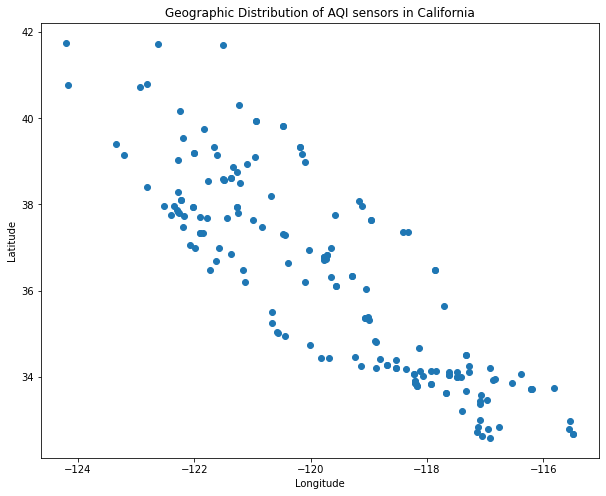
\includegraphics{notebooks/W03. Spatial Data_files/figure-pdf/cell-16-output-2.png}

}

\end{figure}

If you close your eyes and imagine the shape of California, you can
probably see its outline roughly traced in the points above. This plot
leaves a number of things to be desired.

\hypertarget{basemaps}{%
\subsection{Basemaps}\label{basemaps}}

First, we may want to add in a base map of some kind so we can have a
better sense of where each sensor is. For this, we have to import an
extra library called ``Basemap''

\begin{Shaded}
\begin{Highlighting}[]
\CommentTok{\# import Basemap library}
\ImportTok{from}\NormalTok{ mpl\_toolkits.basemap }\ImportTok{import}\NormalTok{ Basemap}

\CommentTok{\# create a basemap, call it \textquotesingle{}map\textquotesingle{}}
\BuiltInTok{map} \OperatorTok{=}\NormalTok{ Basemap(projection}\OperatorTok{=}\StringTok{\textquotesingle{}lcc\textquotesingle{}}\NormalTok{, resolution}\OperatorTok{=}\StringTok{\textquotesingle{}l\textquotesingle{}}\NormalTok{, }\CommentTok{\# this selects the projection of the map.}
\NormalTok{            lat\_0}\OperatorTok{=}\FloatTok{37.5}\NormalTok{, lon\_0}\OperatorTok{={-}}\DecValTok{119}\NormalTok{, }\CommentTok{\# this sets the center of the map }
\NormalTok{            width}\OperatorTok{=}\FloatTok{1E6}\NormalTok{, height}\OperatorTok{=}\FloatTok{1.2E6}\NormalTok{) }\CommentTok{\# this sets the window that we\textquotesingle{}re looking at, in meters.}

\CommentTok{\# We can add features to our blank basemap, including coastlines, as well as state and country boundaries. }
\BuiltInTok{map}\NormalTok{.drawcoastlines(color}\OperatorTok{=}\StringTok{\textquotesingle{}black\textquotesingle{}}\NormalTok{)}
\BuiltInTok{map}\NormalTok{.drawcountries(color}\OperatorTok{=}\StringTok{\textquotesingle{}black\textquotesingle{}}\NormalTok{)}
\BuiltInTok{map}\NormalTok{.drawstates(color}\OperatorTok{=}\StringTok{\textquotesingle{}gray\textquotesingle{}}\NormalTok{)}

\CommentTok{\# Finally, we add in our AQI sensor data on top of the basemap.}
\BuiltInTok{map}\NormalTok{.scatter(}
\NormalTok{    one\_day[}\StringTok{\textquotesingle{}longitude\textquotesingle{}}\NormalTok{], }
\NormalTok{    one\_day[}\StringTok{\textquotesingle{}latitude\textquotesingle{}}\NormalTok{], }
\NormalTok{    latlon}\OperatorTok{=}\VariableTok{True}\NormalTok{)}

\CommentTok{\# as always, title your figure}
\NormalTok{plt.title(}\StringTok{"Geographic Distribution of AQI sensors in California"}\NormalTok{)}
\end{Highlighting}
\end{Shaded}

\begin{verbatim}
ImportError: dlopen(/Users/ollieballinger/miniconda3/envs/geo/lib/python3.9/site-packages/_geoslib.cpython-39-darwin.so, 0x0002): tried: '/Users/ollieballinger/miniconda3/envs/geo/lib/python3.9/site-packages/_geoslib.cpython-39-darwin.so' (mach-o file, but is an incompatible architecture (have 'x86_64', need 'arm64')), '/System/Volumes/Preboot/Cryptexes/OS/Users/ollieballinger/miniconda3/envs/geo/lib/python3.9/site-packages/_geoslib.cpython-39-darwin.so' (no such file), '/Users/ollieballinger/miniconda3/envs/geo/lib/python3.9/site-packages/_geoslib.cpython-39-darwin.so' (mach-o file, but is an incompatible architecture (have 'x86_64', need 'arm64'))
\end{verbatim}

That's looking a bit better! We now have a much better sense of the
actual distribution of these sensors within california. People who know
the area will recognize clusters of sensors around San Francisco and Los
Angeles; This makes sense, given that these areas have a higher
population density. However, our plot is still missing some pretty
important information: the actual AQI readings!

\hypertarget{colormaps}{%
\subsection{Colormaps}\label{colormaps}}

The whole point of plotting these sensors is to understand the spatial
distribution of air pollution from the 2020 wildfires.

The EPA published the following
\href{https://www.airnow.gov/aqi/aqi-basics/}{table} on their website,
which creates a color-coded scale of AQI values that corresponds to the
impact thereof on human health.

\begin{itemize}
\tightlist
\item
  AQI under 50 is colored green, and indicates ``Good'' air quality.
\item
  AQI between 100 and 200 is generally unhealthy
\item
  AQI over 300 is deemed hazardous.
\end{itemize}

With this in mind, quickly scroll back up to the AQI plots over time. If
you did everything correctly, you should notice that the \emph{average}
AQI value across all sensors in the worst affected county was over 600!

We'll be using the table from the EPA website to build our own color
map. In the code below, I scrape the table and turn it into a
``colormap'' (basically, a dictionary that associates numbers with
colors) that we'll use to color the AQI sensors later.

\begin{Shaded}
\begin{Highlighting}[]
\CommentTok{\# scrape the table of AQI values and corresponding colors }
\CommentTok{\# save it as a dataframe called colors}
\NormalTok{colors}\OperatorTok{=}\NormalTok{pd.read\_html(}\StringTok{\textquotesingle{}https://www.airnow.gov/aqi/aqi{-}basics/\textquotesingle{}}\NormalTok{)[}\DecValTok{0}\NormalTok{]}

\CommentTok{\# create a numerical column for AQI values by splitting the test in the "values of index" column. }
\CommentTok{\# pull out the first string, and convert it to integer}
\NormalTok{colors[}\StringTok{\textquotesingle{}aqi\textquotesingle{}}\NormalTok{]}\OperatorTok{=}\NormalTok{colors[}\StringTok{\textquotesingle{}Values of Index\textquotesingle{}}\NormalTok{].}\BuiltInTok{str}\NormalTok{.split(}\StringTok{\textquotesingle{} \textquotesingle{}}\NormalTok{).}\BuiltInTok{str}\NormalTok{[}\DecValTok{0}\NormalTok{].astype(}\BuiltInTok{int}\NormalTok{)}

\CommentTok{\# print three columns from the dataframe }
\BuiltInTok{print}\NormalTok{(colors[[}\StringTok{\textquotesingle{}aqi\textquotesingle{}}\NormalTok{,}\StringTok{\textquotesingle{}Daily AQI Color\textquotesingle{}}\NormalTok{,}\StringTok{\textquotesingle{}Levels of Concern\textquotesingle{}}\NormalTok{]])}

\CommentTok{\# create a "colormap" from this dataframe using the "Daily AQI Color" column, and the "aqi" column }
\NormalTok{aqi\_colors}\OperatorTok{=}\NormalTok{matplotlib.colors.LinearSegmentedColormap.from\_list(colors[}\StringTok{\textquotesingle{}aqi\textquotesingle{}}\NormalTok{],colors[}\StringTok{\textquotesingle{}Daily AQI Color\textquotesingle{}}\NormalTok{])}
\end{Highlighting}
\end{Shaded}

\begin{verbatim}
   aqi Daily AQI Color               Levels of Concern
0    0           Green                            Good
1   51          Yellow                        Moderate
2  101          Orange  Unhealthy for Sensitive Groups
3  151             Red                       Unhealthy
4  201          Purple                  Very Unhealthy
5  301          Maroon                       Hazardous
\end{verbatim}

Now, we can use this ``aqi\_colors'' object as a color palette later
when we plot the AQI sensors. This way, we will know that green and
yellow points are OK, while red and purple points represent hazardous
levels of air pollution. I've annotated the code above, but it's ok if
you don't get all of it. You could simply load a different colormap in
one line of code; check out the documentation
\href{https://matplotlib.org/stable/tutorials/colors/colormaps.html}{here}.

\begin{Shaded}
\begin{Highlighting}[]
\BuiltInTok{map} \OperatorTok{=}\NormalTok{ Basemap(projection}\OperatorTok{=}\StringTok{\textquotesingle{}lcc\textquotesingle{}}\NormalTok{, resolution}\OperatorTok{=}\StringTok{\textquotesingle{}l\textquotesingle{}}\NormalTok{, }
\NormalTok{            lat\_0}\OperatorTok{=}\FloatTok{37.5}\NormalTok{, lon\_0}\OperatorTok{={-}}\DecValTok{119}\NormalTok{,}
\NormalTok{            width}\OperatorTok{=}\FloatTok{1E6}\NormalTok{, height}\OperatorTok{=}\FloatTok{1.2E6}\NormalTok{)}

\BuiltInTok{map}\NormalTok{.drawcoastlines(color}\OperatorTok{=}\StringTok{\textquotesingle{}black\textquotesingle{}}\NormalTok{)}
\BuiltInTok{map}\NormalTok{.drawcountries(color}\OperatorTok{=}\StringTok{\textquotesingle{}black\textquotesingle{}}\NormalTok{)}
\BuiltInTok{map}\NormalTok{.drawstates(color}\OperatorTok{=}\StringTok{\textquotesingle{}gray\textquotesingle{}}\NormalTok{)}

\BuiltInTok{map}\NormalTok{.scatter(}
\NormalTok{      one\_day[}\StringTok{\textquotesingle{}longitude\textquotesingle{}}\NormalTok{], }
\NormalTok{      one\_day[}\StringTok{\textquotesingle{}latitude\textquotesingle{}}\NormalTok{], }
\NormalTok{      latlon}\OperatorTok{=}\VariableTok{True}\NormalTok{, }
\NormalTok{      c}\OperatorTok{=}\NormalTok{one\_day[}\StringTok{\textquotesingle{}AQI\textquotesingle{}}\NormalTok{], }\CommentTok{\# We\textquotesingle{}re adding that }
\NormalTok{      cmap}\OperatorTok{=}\NormalTok{aqi\_colors, }
\NormalTok{      vmin}\OperatorTok{=}\DecValTok{0}\NormalTok{, }
\NormalTok{      vmax}\OperatorTok{=}\DecValTok{300}\NormalTok{)}


\NormalTok{plt.title(}\StringTok{\textquotesingle{}Air Quality on September 9th, 2020\textquotesingle{}}\NormalTok{)}
\NormalTok{plt.colorbar(label}\OperatorTok{=}\StringTok{\textquotesingle{}Air Quality Index\textquotesingle{}}\NormalTok{)}\OperatorTok{;}
\end{Highlighting}
\end{Shaded}

\begin{figure}[H]

{\centering \includegraphics{notebooks/W03. Spatial Data_files/figure-pdf/cell-19-output-1.png}

}

\end{figure}

This plot gives us a good sense of which areas were worst affected by
the wildfires on September 9th, 2020. Areas in the central valley
suffered particularly bad air quality, with AQI reaching hazardous
levels in some areas.

\hypertarget{exercise-6}{%
\subsection{Exercise}\label{exercise-6}}

So far, we've been plotting data from one day, using a dataframe we
generated by filtering the date column like so:
\texttt{one\_day=df{[}df{[}\textquotesingle{}Date\textquotesingle{}{]}==\textquotesingle{}09-09-2020\textquotesingle{}{]}}
(date format is day-month-year).

Using the code from the previous cell, generate a plot of AQI on March
2nd, 2020. After that, use the groupby function to generate a plot of
the maximum AQI reading for each sensor and plot it.

If you've followed along this far, well done! we've come a long way from
a spreadsheet full of sensor readings. But we can go even further!

\hypertarget{advanced-satellite-imagery-and-interactivity}{%
\section{Advanced: Satellite Imagery and
Interactivity}\label{advanced-satellite-imagery-and-interactivity}}

The AQI plots we've generated above give us a good sense of where the
worst air pollution was on a given day; but we're still basically
\emph{inferring} the presence of fires. Luckily, we don't have to do
that. The plumes of smoke generated by the fires were so vast that they
were visible from space. There are a variety of satellites that image
the earth each day (some, like GOES-17, take a picture every few
minutes!).

NASA's Moderate Resolution Imaging Spectroradiometer (MODIS) satellites
take a picture of the same spot on earth nearly every day. So far, we've
been looking at September 9th as a particularly bad day for air quality
in California. Let's have a look at a satellite image from that day. A
Python library called ipyleaflet contains some useful functions that let
us pull up an interactive map of satellite imagery.

\begin{Shaded}
\begin{Highlighting}[]
\CommentTok{\# import the map making modules from ipyleaflet}
\ImportTok{from}\NormalTok{ ipyleaflet }\ImportTok{import}\NormalTok{ Map, Marker, basemaps, basemap\_to\_tiles,Circle}
\ImportTok{from}\NormalTok{ ipywidgets }\ImportTok{import}\NormalTok{ HTML}

\CommentTok{\# let create an interactive Map object called "satellite\_map"}
\NormalTok{satellite\_map }\OperatorTok{=}\NormalTok{ Map(}
\NormalTok{  basemap}\OperatorTok{=}\NormalTok{basemap\_to\_tiles( }\CommentTok{\#this function lets us pick from a list of basemaps for our interactive map}
\NormalTok{    basemaps.NASAGIBS.ModisTerraTrueColorCR, }\StringTok{"2020{-}09{-}09"} \CommentTok{\# here we\textquotesingle{}re specifying that we want MODIS imagery, and the date that we want it from  }
\NormalTok{  ),}
\NormalTok{  center}\OperatorTok{=}\NormalTok{(}\FloatTok{36.77}\NormalTok{, }\OperatorTok{{-}}\FloatTok{119.41}\NormalTok{), }\CommentTok{\# then, we want to center the map on california. these coordinates do that}
\NormalTok{  zoom}\OperatorTok{=}\DecValTok{5}\NormalTok{, }\CommentTok{\#finally, we want to set the zoom level of the map. }
\NormalTok{)}

\CommentTok{\# once we\textquotesingle{}ve created the map object we can make it bigger or smaller. let\textquotesingle{}s make it 700 pixels tall. }
\NormalTok{satellite\_map.layout.height }\OperatorTok{=} \StringTok{\textquotesingle{}700px\textquotesingle{}}

\CommentTok{\# now, we visualize it.}
\NormalTok{satellite\_map}
\end{Highlighting}
\end{Shaded}

\begin{verbatim}
Map(center=[36.77, -119.41], controls=(ZoomControl(options=['position', 'zoom_in_text', 'zoom_in_title', 'zoom…
\end{verbatim}

This is a pretty striking image of the West Coast of the U.S. We can see
fluffy white clouds to the East and West, but in the center of the map
plumes of brown smoke emanate from wildfires in California and Oregon.
Use the + - keys in the top left to zoom in, see if you can spot some
wildfires.

\hypertarget{exercise-7}{%
\subsection{Exercise}\label{exercise-7}}

Try changing the code in the cell above to display an image from
September 15th. You could even try importing a different basemap (like
nighttime lights) using this
\href{https://ipyleaflet.readthedocs.io/en/latest/map_and_basemaps/basemaps.html}{list
of basemaps}.

\hypertarget{combining-sensors-and-satellite-images}{%
\section{Combining sensors and satellite
images}\label{combining-sensors-and-satellite-images}}

A cool part of working with spatial data is that we can combine two
completeley different datasets using spatial information. We can add the
AQI sensor data as points to this map.

\begin{Shaded}
\begin{Highlighting}[]
\CommentTok{\# grab the first row from our September 9th dataframe}
\NormalTok{row}\OperatorTok{=}\NormalTok{one\_day.iloc[}\DecValTok{0}\NormalTok{]}
\BuiltInTok{print}\NormalTok{(row)}

\CommentTok{\# This part uses the AQI value in this row (72), and looks up the corresponding color in the colormap we created earlier }
\NormalTok{color}\OperatorTok{=}\NormalTok{matplotlib.colors.rgb2hex(aqi\_colors(row[}\StringTok{\textquotesingle{}AQI\textquotesingle{}}\NormalTok{]))}

\CommentTok{\# Now we create a Circle object using the latitude and longitude from the row, and color it using the color we just selected}
\NormalTok{point}\OperatorTok{=}\NormalTok{Circle(location}\OperatorTok{=}\NormalTok{(row[}\StringTok{\textquotesingle{}latitude\textquotesingle{}}\NormalTok{],row[}\StringTok{\textquotesingle{}longitude\textquotesingle{}}\NormalTok{]), color}\OperatorTok{=}\NormalTok{color)}

\CommentTok{\# Add this as a layer to the satellite\_map object}
\NormalTok{satellite\_map.add\_layer(point)}

\CommentTok{\# Display the updated map}
\NormalTok{satellite\_map}
\end{Highlighting}
\end{Shaded}

\begin{verbatim}
Date                       2020-09-09 00:00:00
Site ID                               60010007
POC                                          3
PM                                        22.3
AQI                                         72
Site Name                            Livermore
CBSA_NAME    San Francisco-Oakland-Hayward, CA
COUNTY                                 Alameda
latitude                             37.687526
longitude                          -121.784217
Month                                        9
Day                                        253
Name: 249, dtype: object
\end{verbatim}

\begin{verbatim}
Map(center=[36.77, -119.41], controls=(ZoomControl(options=['position', 'zoom_in_text', 'zoom_in_title', 'zoom…
\end{verbatim}

It's a bit hard to see, but we've plotted an AQI sensor! its under the
cloud of smoke in the center of the map. You can zoom in to get a closer
look. looks like AQI was pretty bad at this location.

Having plotted one point, we can now plot all the points on September
9th! to do so, we can use the \texttt{iterrows} function in Pandas
which, suprisingly, lets you iterate over rows in a dataframe. The first
line of code below allows us to iterate over the rows in the
\texttt{one\_day} dataframe. It will then run everything in the indented
block for each row; in other words, for each row, it will:

\begin{enumerate}
\def\labelenumi{\arabic{enumi}.}
\tightlist
\item
  use the row's value in the AQI value to select a color for the point
\item
  create a point object using the latitude and longitude columns
\item
  add that point to the satellite map.
\end{enumerate}

\begin{Shaded}
\begin{Highlighting}[]
\ControlFlowTok{for}\NormalTok{ index, row }\KeywordTok{in}\NormalTok{ one\_day.iterrows():}
\NormalTok{  color}\OperatorTok{=}\NormalTok{matplotlib.colors.rgb2hex(aqi\_colors(row[}\StringTok{\textquotesingle{}AQI\textquotesingle{}}\NormalTok{]))}
\NormalTok{  point}\OperatorTok{=}\NormalTok{Circle(location}\OperatorTok{=}\NormalTok{(row[}\StringTok{\textquotesingle{}latitude\textquotesingle{}}\NormalTok{],row[}\StringTok{\textquotesingle{}longitude\textquotesingle{}}\NormalTok{]), color}\OperatorTok{=}\NormalTok{color)}
\NormalTok{  satellite\_map.add\_layer(point)}

\CommentTok{\# display the map}
\NormalTok{satellite\_map}
\end{Highlighting}
\end{Shaded}

\begin{verbatim}
Map(center=[36.77, -119.41], controls=(ZoomControl(options=['position', 'zoom_in_text', 'zoom_in_title', 'zoom…
\end{verbatim}

Theres a pretty striking trend in this data. If you zoom in, you'll see
that the AQI sensors to the East are all green since they are up-wind
from the fires. A few kilometers downwind of the fires, the AQI sensors
display very high readings. Remember, our AQI data and the satellite
imagery are derived from totally different sources, and are totally
different types of data, but they seem to be telling us the same story.
They actually complement each other in important ways. In our original
plot of the AQI sensors without satellite imagery, we could tell that
there was bad air quality on September 9th, but some sensors were green
and others were red. The satellite image shows us that the variation in
AQI across California on September 9th was due to the direction of the
wind, blowing the smoke from the wildfires westward.

\hypertarget{extension-1}{%
\section{Extension}\label{extension-1}}

Now, to save some hassle we can package all the code we used to generate
this map into one clean function. Because we're effectively just
changing the date, we can configure this function so that we can feed it
a different date, and it will grab a satellite image and filter our
dataframe for values occuring on that day. Then, we can draw a new map
in one line of code.

\begin{Shaded}
\begin{Highlighting}[]
\KeywordTok{def}\NormalTok{ satellite\_plot(date):}
  
\NormalTok{  ymd}\OperatorTok{=}\NormalTok{datetime.strptime(date, }\StringTok{\textquotesingle{}}\SpecialCharTok{\%d}\StringTok{{-}\%m{-}\%Y\textquotesingle{}}\NormalTok{).strftime(}\StringTok{\textquotesingle{}\%Y{-}\%m{-}}\SpecialCharTok{\%d}\StringTok{\textquotesingle{}}\NormalTok{)}

\NormalTok{  satellite\_map }\OperatorTok{=}\NormalTok{ Map(}
\NormalTok{    basemap}\OperatorTok{=}\NormalTok{basemap\_to\_tiles(}
\NormalTok{      basemaps.NASAGIBS.ModisTerraTrueColorCR, ymd}
\NormalTok{    ),}
\NormalTok{    center}\OperatorTok{=}\NormalTok{(}\FloatTok{36.77}\NormalTok{, }\OperatorTok{{-}}\FloatTok{119.41}\NormalTok{),}
\NormalTok{    zoom}\OperatorTok{=}\DecValTok{6}\NormalTok{,}
\NormalTok{  )}

\NormalTok{  satellite\_map.layout.height }\OperatorTok{=} \StringTok{\textquotesingle{}700px\textquotesingle{}}

\NormalTok{  one\_day}\OperatorTok{=}\NormalTok{df[df[}\StringTok{\textquotesingle{}Date\textquotesingle{}}\NormalTok{]}\OperatorTok{==}\NormalTok{date]}

  \ControlFlowTok{for}\NormalTok{ index, row }\KeywordTok{in}\NormalTok{ one\_day.iterrows():}
\NormalTok{    color}\OperatorTok{=}\NormalTok{matplotlib.colors.rgb2hex(aqi\_colors(row[}\StringTok{\textquotesingle{}AQI\textquotesingle{}}\NormalTok{]))}
\NormalTok{    point}\OperatorTok{=}\NormalTok{Circle(location}\OperatorTok{=}\NormalTok{(row[}\StringTok{\textquotesingle{}latitude\textquotesingle{}}\NormalTok{],row[}\StringTok{\textquotesingle{}longitude\textquotesingle{}}\NormalTok{]), color}\OperatorTok{=}\NormalTok{color)}
\NormalTok{    point.popup }\OperatorTok{=}\NormalTok{ HTML(}\BuiltInTok{str}\NormalTok{(row[}\StringTok{\textquotesingle{}Site Name\textquotesingle{}}\NormalTok{]))    }
\NormalTok{    satellite\_map.add\_layer(point)}
  \ControlFlowTok{return}\NormalTok{ satellite\_map}
\end{Highlighting}
\end{Shaded}

Now, we can simply change the date in the function and view both
satellite imagery and AQI sensor data from a given day. Look at this
clear day from February 3rd.

\begin{Shaded}
\begin{Highlighting}[]
\NormalTok{satellite\_plot(}\StringTok{\textquotesingle{}02{-}03{-}2020\textquotesingle{}}\NormalTok{)}
\end{Highlighting}
\end{Shaded}

\begin{verbatim}
Map(center=[36.77, -119.41], controls=(ZoomControl(options=['position', 'zoom_in_text', 'zoom_in_title', 'zoom…
\end{verbatim}

All the AQI sensors are showing green values, indicating generally good
air quality. The satellite image shows a few wispy clouds, but no thick
yellow smoke. Now change the date to September 15th, and see what
happens!

\bookmarksetup{startatroot}

\hypertarget{natural-language-processing}{%
\chapter{Natural Language
Processing}\label{natural-language-processing}}

\hypertarget{workshop-4-open-in-colab}{%
\section[\emph{Workshop 4} ]{\texorpdfstring{\emph{Workshop 4}
\href{https://colab.research.google.com/github/oballinger/QM2/blob/main/notebooks/W04.\%20Natural\%20Language\%20Processing.ipynb}{\protect
\includegraphics{index_files/mediabag/colab-badge.png}}}{Workshop 4 Open In Colab}}\label{workshop-4-open-in-colab}}

\hypertarget{background-1}{%
\section{Background}\label{background-1}}

Exxon Mobil is the 4th largest oil company in the world. In 1978, an
Exxon scientist named James Black wrote an
\href{https://insideclimatenews.org/documents/james-black-1977-presentation/}{internal
briefing} called ``The Greenhouse Effect'' in which he warned: ``Present
thinking holds that man has a time window of five to ten years before
the need for hard decisions regarding changes in energy strategies might
become critical.''

Rather than acting on this information, Exxon spent the next
\href{https://news.harvard.edu/gazette/story/2021/09/oil-companies-discourage-climate-action-study-says/}{forty
years aggressively funding climate denial}. Recently,
\href{https://www.theguardian.com/environment/2022/may/24/exxon-trial-climate-crimes-fossil-fuels-global-heating}{a
U.S. court ruled} that ExxonMobil must face trial over accusations that
it lied about the climate crisis and covered up the fossil fuel
industry's role in worsening environmental devastation.

\hypertarget{earnings-calls}{%
\subsection{Earnings Calls}\label{earnings-calls}}

Every three months, Exxon conducts an
\href{https://www.investopedia.com/terms/e/earnings-call.asp}{``earnings
call''}; a conference call between the management of a public company,
analysts, investors, and the media to discuss the company's financial
results during a given reporting period, such as a quarter or a fiscal
year.

You can
\href{https://globalmeet.webcasts.com/starthere.jsp?ei=1488251\&tp_key=440e363aaf}{register}
to attend their next one if you want! No worries if you miss it, they
provide
\href{https://corporate.exxonmobil.com/Investors/Investor-relations/Investor-materials-archive\#Quarterlyearningsmaterials}{transcripts}
on their website.

These transcripts provide an intimate window into the company's
dealings. We can see how much pressure investors are putting on the
company to tackle climate change, and how the company responds.

We'll be working with transcripts spanning nealry 20 years and over 10
million words; that's like reading the Harry Potter series 10 times.
Then, we'll look at a sample of 100,000 tweets that use the \#ExxonKnew
hashtag, and analyze public pressure on the company.

\includegraphics{index_files/mediabag/business.jpg}

\hypertarget{downloading-the-data-1}{%
\section{Downloading the Data}\label{downloading-the-data-1}}

Let's grab the data we will need this week from our course website and
save it into our data folder. If you've not already created a data
folder then do so using the following command.

Don't worry if it generates an error, that means you've already got a
data folder.

\begin{Shaded}
\begin{Highlighting}[]
\OperatorTok{\%\%}\NormalTok{capture}
\OperatorTok{!}\NormalTok{pip install spacy}
\OperatorTok{!}\NormalTok{pip install scattertext}
\OperatorTok{!}\NormalTok{pip install tika}
\OperatorTok{!}\NormalTok{pip install spacytextblob}
\end{Highlighting}
\end{Shaded}

\begin{Shaded}
\begin{Highlighting}[]
\CommentTok{\#Make a ./data/wk4 directory}
\OperatorTok{!}\NormalTok{mkdir data}
\OperatorTok{!}\NormalTok{mkdir data}\OperatorTok{/}\NormalTok{wk4}
\end{Highlighting}
\end{Shaded}

\begin{verbatim}
mkdir: data: File exists
mkdir: data/wk4: File exists
\end{verbatim}

\begin{Shaded}
\begin{Highlighting}[]
\OperatorTok{!}\NormalTok{curl https:}\OperatorTok{//}\NormalTok{storage.googleapis.com}\OperatorTok{/}\NormalTok{qm2}\OperatorTok{/}\NormalTok{wk4}\OperatorTok{/}\NormalTok{Exxon.json }\OperatorTok{{-}}\NormalTok{o data}\OperatorTok{/}\NormalTok{wk4}\OperatorTok{/}\NormalTok{Exxon.json}
\end{Highlighting}
\end{Shaded}

\begin{verbatim}
  % Total    % Received % Xferd  Average Speed   Time    Time     Time  Current
                                 Dload  Upload   Total   Spent    Left  Speed
100 10.5M  100 10.5M    0     0  13.1M      0 --:--:-- --:--:-- --:--:-- 13.2M
\end{verbatim}

\begin{Shaded}
\begin{Highlighting}[]
\ImportTok{import}\NormalTok{ spacy}
\ImportTok{import}\NormalTok{ json}
\ImportTok{import}\NormalTok{ pylab}
\ImportTok{from}\NormalTok{ IPython.core.display }\ImportTok{import}\NormalTok{ display, HTML}
\ImportTok{import}\NormalTok{ nltk}
\ImportTok{from}\NormalTok{ tika }\ImportTok{import}\NormalTok{ parser}
\ImportTok{import}\NormalTok{ numpy }\ImportTok{as}\NormalTok{ np}
\ImportTok{import}\NormalTok{ pandas }\ImportTok{as}\NormalTok{ pd}
\ImportTok{import}\NormalTok{ matplotlib.pyplot }\ImportTok{as}\NormalTok{ plt}
\ImportTok{from}\NormalTok{ spacytextblob.spacytextblob }\ImportTok{import}\NormalTok{ SpacyTextBlob}

\OperatorTok{\%}\NormalTok{matplotlib inline}
\NormalTok{pylab.rcParams[}\StringTok{\textquotesingle{}figure.figsize\textquotesingle{}}\NormalTok{] }\OperatorTok{=}\NormalTok{ (}\FloatTok{10.}\NormalTok{, }\FloatTok{8.}\NormalTok{)}
\NormalTok{nlp }\OperatorTok{=}\NormalTok{ spacy.load(}\StringTok{"en\_core\_web\_sm"}\NormalTok{)}
\NormalTok{nlp.add\_pipe(}\StringTok{\textquotesingle{}spacytextblob\textquotesingle{}}\NormalTok{)}
\end{Highlighting}
\end{Shaded}

\begin{verbatim}
TypeError: Descriptors cannot not be created directly.
If this call came from a _pb2.py file, your generated code is out of date and must be regenerated with protoc >= 3.19.0.
If you cannot immediately regenerate your protos, some other possible workarounds are:
 1. Downgrade the protobuf package to 3.20.x or lower.
 2. Set PROTOCOL_BUFFERS_PYTHON_IMPLEMENTATION=python (but this will use pure-Python parsing and will be much slower).

More information: https://developers.google.com/protocol-buffers/docs/news/2022-05-06#python-updates
\end{verbatim}

\hypertarget{downloading-and-reading-one-earnings-call}{%
\section{Downloading and reading one earnings
call}\label{downloading-and-reading-one-earnings-call}}

Exxon host earnings calls on their website in PDF form. Usually, working
with PDFs is a real pain as they are not machine-readable. Using a
python package called
\href{https://www.geeksforgeeks.org/parsing-pdfs-in-python-with-tika/}{tika},
we can ``parse'' a pdf, turning it into machine-readable text:

\begin{Shaded}
\begin{Highlighting}[]
\CommentTok{\# define the URL where your PDF lives. You could also upload your own pdf.}
\CommentTok{\#url=\textquotesingle{}https://corporate.exxonmobil.com/{-}/media/Global/Files/investor{-}relations/quarterly{-}earnings/earnings{-}transcripts/2022{-}earnings{-}transcripts/1Q22{-}XOM{-}Earnings{-}Call{-}Transcript{-}4{-}29{-}22.pdf\textquotesingle{}}
\NormalTok{url}\OperatorTok{=}\StringTok{\textquotesingle{}https://d1io3yog0oux5.cloudfront.net/\_74d009918ead0ec6acdd6bbaf27a8316/exxonmobil/db/2288/22123/earnings\_release/XOM+2Q23+Earnings+Press+Release+Website.pdf\textquotesingle{}}
\CommentTok{\# parse the pdf by feeding tika the URL and store the text in an object called "raw" }
\NormalTok{raw }\OperatorTok{=}\NormalTok{ parser.from\_file(url)}
\end{Highlighting}
\end{Shaded}

\begin{verbatim}
2022-10-27 08:18:46,398 [MainThread  ] [INFO ]  Retrieving https://corporate.exxonmobil.com/-/media/Global/Files/investor-relations/quarterly-earnings/earnings-transcripts/2022-earnings-transcripts/1Q22-XOM-Earnings-Call-Transcript-4-29-22.pdf to /tmp/media-global-files-investor-relations-quarterly-earnings-earnings-transcripts-2022-earnings-transcripts-1q22-xom-earnings-call-transcript-4-29-22.pdf.
INFO:tika.tika:Retrieving https://corporate.exxonmobil.com/-/media/Global/Files/investor-relations/quarterly-earnings/earnings-transcripts/2022-earnings-transcripts/1Q22-XOM-Earnings-Call-Transcript-4-29-22.pdf to /tmp/media-global-files-investor-relations-quarterly-earnings-earnings-transcripts-2022-earnings-transcripts-1q22-xom-earnings-call-transcript-4-29-22.pdf.
2022-10-27 08:18:46,901 [MainThread  ] [INFO ]  Retrieving http://search.maven.org/remotecontent?filepath=org/apache/tika/tika-server/1.24/tika-server-1.24.jar to /tmp/tika-server.jar.
INFO:tika.tika:Retrieving http://search.maven.org/remotecontent?filepath=org/apache/tika/tika-server/1.24/tika-server-1.24.jar to /tmp/tika-server.jar.
2022-10-27 08:18:47,623 [MainThread  ] [INFO ]  Retrieving http://search.maven.org/remotecontent?filepath=org/apache/tika/tika-server/1.24/tika-server-1.24.jar.md5 to /tmp/tika-server.jar.md5.
INFO:tika.tika:Retrieving http://search.maven.org/remotecontent?filepath=org/apache/tika/tika-server/1.24/tika-server-1.24.jar.md5 to /tmp/tika-server.jar.md5.
2022-10-27 08:18:48,084 [MainThread  ] [WARNI]  Failed to see startup log message; retrying...
WARNING:tika.tika:Failed to see startup log message; retrying...
2022-10-27 08:18:53,099 [MainThread  ] [WARNI]  Failed to see startup log message; retrying...
WARNING:tika.tika:Failed to see startup log message; retrying...
\end{verbatim}

Now, we have an object called ``raw'' that contains some useful
information. Notice the squiggly brackets; this is a dictionary. It
contains several fields, including some useful metadata such as the
author

\begin{Shaded}
\begin{Highlighting}[]
\NormalTok{date}\OperatorTok{=}\NormalTok{raw[}\StringTok{\textquotesingle{}metadata\textquotesingle{}}\NormalTok{][}\StringTok{\textquotesingle{}date\textquotesingle{}}\NormalTok{]}
\NormalTok{title}\OperatorTok{=}\NormalTok{raw[}\StringTok{\textquotesingle{}metadata\textquotesingle{}}\NormalTok{][}\StringTok{\textquotesingle{}dc:title\textquotesingle{}}\NormalTok{]}
\NormalTok{raw\_text}\OperatorTok{=}\NormalTok{raw[}\StringTok{\textquotesingle{}content\textquotesingle{}}\NormalTok{]}

\BuiltInTok{print}\NormalTok{(}\StringTok{\textquotesingle{}Date: \textquotesingle{}}\NormalTok{, date)}
\BuiltInTok{print}\NormalTok{(}\StringTok{\textquotesingle{}Title: \textquotesingle{}}\NormalTok{, title)}
\BuiltInTok{print}\NormalTok{(}\StringTok{\textquotesingle{}Word Count: \textquotesingle{}}\NormalTok{, }\BuiltInTok{len}\NormalTok{(raw\_text))}
\BuiltInTok{print}\NormalTok{(}\StringTok{\textquotesingle{}Text:\textquotesingle{}}\NormalTok{)}
\NormalTok{raw\_text}
\end{Highlighting}
\end{Shaded}

look at that! we're beginning to give some structure to our text data.
But suppose I wanted to analyze multiple earnings calls; I need to
organize this data so that it can accomodate new entries. As always, we
want to \textbf{tabularize} our data. Let's create a dataframe with
three columns (Date, Title, and Text) in which each row is one earnings
call:

\begin{Shaded}
\begin{Highlighting}[]
\CommentTok{\# create a dataframe using the above data }
\NormalTok{call}\OperatorTok{=}\NormalTok{pd.DataFrame(\{}\StringTok{\textquotesingle{}Date\textquotesingle{}}\NormalTok{:[date],}\StringTok{\textquotesingle{}Title\textquotesingle{}}\NormalTok{:[title],}\StringTok{\textquotesingle{}Text\textquotesingle{}}\NormalTok{:[raw\_text]\})}

\CommentTok{\# remember, datetime information almost always reaches us as text. }
\CommentTok{\# we need to explicitly convert it to the datetime data type. }
\NormalTok{call[}\StringTok{\textquotesingle{}Date\textquotesingle{}}\NormalTok{]}\OperatorTok{=}\NormalTok{pd.to\_datetime(call[}\StringTok{\textquotesingle{}Date\textquotesingle{}}\NormalTok{], infer\_datetime\_format}\OperatorTok{=}\VariableTok{True}\NormalTok{)}

\CommentTok{\# Let\textquotesingle{}s see what we\textquotesingle{}ve got.}
\NormalTok{call}
\end{Highlighting}
\end{Shaded}

\begin{longtable}[]{@{}llll@{}}
\toprule\noalign{}
& Date & Title & Text \\
\midrule\noalign{}
\endhead
\bottomrule\noalign{}
\endlastfoot
0 & 2022-05-04 16:51:56 & 1Q22 XOM Earnings Call Transcript 4-29-22 &
\textbackslash n\textbackslash n\textbackslash n\textbackslash n\textbackslash n\textbackslash n\textbackslash n\textbackslash n\textbackslash n\textbackslash n\textbackslash n\textbackslash n\textbackslash n\textbackslash n\textbackslash n\textbackslash n\textbackslash n\textbackslash n\textbackslash n\textbackslash n\textbackslash n\textbackslash n\textbackslash n... \\
\end{longtable}

Now, if we were so inclined, we could use a loop to repeat this process
for a large number of earnings calls, yielding a neatly organized
dataframe containing the date, title, and text of earnings calls over
time. I've done this so you don't have to, and stored it as a file
called ``Exxon.json''. It spans 2002-2019, and contains over 10 million
words' worth of earnings calls. Let's take a peek:

\begin{Shaded}
\begin{Highlighting}[]
\NormalTok{df}\OperatorTok{=}\NormalTok{pd.read\_json(}\StringTok{\textquotesingle{}data/wk4/Exxon.json\textquotesingle{}}\NormalTok{)}
\NormalTok{df}
\end{Highlighting}
\end{Shaded}

\begin{longtable}[]{@{}llll@{}}
\toprule\noalign{}
& Title & Date & Text \\
\midrule\noalign{}
\endhead
\bottomrule\noalign{}
\endlastfoot
0 & Exxon Mobil Corp at Barclays CEO EnergyPower ... & 2019-09-04 & Mr.
Woods joined ExxonMobil International in 1... \\
1 & Q2 2019 Exxon Mobil Corp Earnings Call - Final & 2019-08-02 & NEIL
A. HANSEN, VP OF IR \& SECRETARY, EXXON MO... \\
2 & Event Brief of Q2 2019 Exxon Mobil Corp Earn... & 2019-08-02 & .
Neil A. Hansen - Exxon Mobil Corporation,VP ... \\
3 & Exxon Mobil Corp at JPMorgan Energy Conferenc... & 2019-06-18 & So
with that, I\textquotesingle ll turn it over to you. Thank ... \\
4 & Exxon Mobil Corp Annual Shareholders Meeting ... & 2019-05-29 &
DARREN W. WOODS, CHAIRMAN \& CEO, EXXON MOBIL C... \\
... & ... & ... & ... \\
177 & Event Brief of Q3 2002 Exxon Mobil Corporati... & 2002-10-31 &
OVERVIEW \textbackslash n\textbackslash n XOM reported normalized
earnings... \\
178 & Q3 2002 Exxon Mobil Corporation Earnings Con... & 2002-10-31 & In
particular, I refer you to factors affectin... \\
179 & Q2 2002 Exxon Mobil Corporation Earnings Con... & 2002-08-01 &
Welcome to Exxon Mobil\textquotesingle s teleconference and we... \\
180 & Abstract of Q2 2002 Exxon Mobil Corporation ... & 2002-08-01 &
OVERVIEW \textbackslash n\textbackslash n XOM: 2Q02 net income was
\$2.64b.... \\
181 & Exxon Mobil Corporation First Quarter 2002 Re... & 2002-04-23 & We
also signed a memorandum of understanding t... \\
\end{longtable}

Great-- we've got a structured dataset of earnings calls. But even
though the data has \emph{structure}, the data in the ``Text'' column
still needs some cleaning and processing.

\hypertarget{dirty-words}{%
\section{Dirty Words}\label{dirty-words}}

Text often comes `unclean' either containing tags such as HTML (or XML),
or has other issues. We've already done a bit of tidying, but it's been
relatively straightforward. Be cautious when committing to a text
analysis project - you may spend a great deal of time tidying up your
text.

For example, you may have noticed ``\n\n\n\n\n\n\n\n\ldots{}'' in the
text of the first earnings call we downloaded. This is a character (just
like ``a'' or ``\$'') except it indicates that we want to create a new
line. It's part of the formatting of the pdf. That's not really useful
information to us. Let start by selecting an earnings call; i've chosen
the 38th in this dataframe:

\begin{Shaded}
\begin{Highlighting}[]
\NormalTok{call}\OperatorTok{=}\NormalTok{df.iloc[}\DecValTok{38}\NormalTok{]}

\BuiltInTok{print}\NormalTok{(}\StringTok{\textquotesingle{}Date: \textquotesingle{}}\NormalTok{, call[}\StringTok{\textquotesingle{}Date\textquotesingle{}}\NormalTok{])}
\BuiltInTok{print}\NormalTok{(}\StringTok{\textquotesingle{}Title: \textquotesingle{}}\NormalTok{, call[}\StringTok{\textquotesingle{}Title\textquotesingle{}}\NormalTok{])}
\BuiltInTok{print}\NormalTok{(}\StringTok{\textquotesingle{}Word Count: \textquotesingle{}}\NormalTok{, }\BuiltInTok{len}\NormalTok{(call[}\StringTok{\textquotesingle{}Text\textquotesingle{}}\NormalTok{]))}
\BuiltInTok{print}\NormalTok{(}\StringTok{\textquotesingle{}Text:\textquotesingle{}}\NormalTok{)}
\NormalTok{call[}\StringTok{\textquotesingle{}Text\textquotesingle{}}\NormalTok{]}
\end{Highlighting}
\end{Shaded}

This call took place on May 25th, 2016. The transcript is over 125,000
words, nearly as long as the third Lord of the Rings book. It would be a
pain to read all of it, so we'll use python to extract insights.
Currently, the contents of \texttt{call{[}"Text"{]}} is a
\href{https://docs.python.org/3/library/stdtypes.html\#text-sequence-type-str}{``string''}--
a sequence of characters. We can do a number of things with strings,
including splitting a big string into smaller strings using a specific
delimiter and the \texttt{.split()} function. For example, I can break
down the whole text of the earnings call roughly into sentences by
splitting the string every time I encounter a period (``.''). This
returns a list of smaller strings, and if i select the first one using
\texttt{{[}0{]}}, I get the first sentence of this call:

\begin{Shaded}
\begin{Highlighting}[]
\NormalTok{call[}\StringTok{\textquotesingle{}Text\textquotesingle{}}\NormalTok{].split(}\StringTok{\textquotesingle{}.\textquotesingle{}}\NormalTok{)[}\DecValTok{0}\NormalTok{]}
\end{Highlighting}
\end{Shaded}

\begin{verbatim}
"I'm Rex Tillerson, I'm the Chairman and Chief Executive Officer of the Exxon Mobil Corporation"
\end{verbatim}

Lovely! the first sentence is an introduction by then-CEO
\href{https://en.wikipedia.org/wiki/Rex_Tillerson}{Rex Tillerson}.

He was CEO of Exxon from 2006 until he retired on January 1st 2017. One
month later, he was sworn in as U.S. Secretary of State under Donald
Trump. Let's see what Rex thinks about climate change!

\hypertarget{regular-expressions-regex}{%
\section{Regular Expressions (Regex)}\label{regular-expressions-regex}}

Another thing we can do with strings in python is search them using
regular expressions. A regular expression is a sequence of characters
that specifies a search pattern in text. You can play around building
some regex queries using this \href{https://regexr.com/}{tool}.

You can think about this as Ctrl+F on steroids; In its simplest form, we
can use regex to search for a character, word, or phrase in a bunch of
text. For example, we can use regular expressions to count how many
times ``climate change'' is mentioned in this earnings call using the
\texttt{re.findall()} function:

\begin{Shaded}
\begin{Highlighting}[]
\CommentTok{\# import the regular expressions library }
\ImportTok{import}\NormalTok{ re}

\CommentTok{\# use the findall function to search for mentions of "climate change" in the text of our call}
\NormalTok{climate\_change }\OperatorTok{=}\NormalTok{ re.findall(}\VerbatimStringTok{r\textquotesingle{}climate change\textquotesingle{}}\NormalTok{, call[}\StringTok{\textquotesingle{}Text\textquotesingle{}}\NormalTok{], re.IGNORECASE)}

\CommentTok{\# this returns a list of strings matching our search term. }
\CommentTok{\# the length of the list gives us the number of occurances}
\BuiltInTok{len}\NormalTok{(climate\_change)}
\end{Highlighting}
\end{Shaded}

\begin{verbatim}
11
\end{verbatim}

Looks like climate change is mentioned 51 times in this earnings call.

\begin{center}\rule{0.5\linewidth}{0.5pt}\end{center}

\hypertarget{exercise-8}{%
\subsection{Exercise}\label{exercise-8}}

how many times is the phrase ``global warming'' mentioned?

\begin{center}\rule{0.5\linewidth}{0.5pt}\end{center}

But we have 182 earnings calls in this sample-- suppose we want to count
the number of times climate change is mentioned in each one, so we can
see the salience of this topic over time.

\hypertarget{applying-a-lambda-function-to-a-dataframe}{%
\subsection{Applying a lambda function to a
dataframe}\label{applying-a-lambda-function-to-a-dataframe}}

Because each row of our dataframe \texttt{df} is an earnings call (the
text of which is contained in
\texttt{df{[}\textquotesingle{}Text\textquotesingle{}{]}}, we want to
apply the analysis we did for the single earnings call above to each row
of \texttt{df}.

We can accomplish this using a
\href{https://www.w3schools.com/python/python_lambda.asp}{\textbf{lambda
function}}. This allows us to iterate over each value in a dataframe
column, and apply a function to it. In the simple example below, I use a
lambda function to create a new column that is takes the values from a
different column and multiplies them by 2:

\begin{Shaded}
\begin{Highlighting}[]
\CommentTok{\# create a dataframe called "example" with one column called "numbers" which contains numbers 0{-}5}
\NormalTok{example}\OperatorTok{=}\NormalTok{ pd.DataFrame(\{}\StringTok{\textquotesingle{}numbers\textquotesingle{}}\NormalTok{:[}\DecValTok{0}\NormalTok{,}\DecValTok{1}\NormalTok{,}\DecValTok{2}\NormalTok{,}\DecValTok{3}\NormalTok{,}\DecValTok{4}\NormalTok{,}\DecValTok{5}\NormalTok{]\})}

\CommentTok{\# print the dataframe }
\BuiltInTok{print}\NormalTok{(}\StringTok{"}\CharTok{\textbackslash{}n}\StringTok{ Before applying lambda function: }\CharTok{\textbackslash{}n}\StringTok{"}\NormalTok{, example)}

\CommentTok{\# create a new column called "doubled numbers"}
\CommentTok{\# apply a lambda function that iterates over each row in the "numbers" column}
\CommentTok{\# call each row "x", and multiply it by 2}
\NormalTok{example[}\StringTok{\textquotesingle{}doubled numbers\textquotesingle{}}\NormalTok{]}\OperatorTok{=}\NormalTok{ example[}\StringTok{\textquotesingle{}numbers\textquotesingle{}}\NormalTok{].}\BuiltInTok{apply}\NormalTok{(}\KeywordTok{lambda}\NormalTok{ x: x}\OperatorTok{*}\DecValTok{2}\NormalTok{)}

\CommentTok{\# print the dataframe, which now contains the new column}
\BuiltInTok{print}\NormalTok{(}\StringTok{"}\CharTok{\textbackslash{}n}\StringTok{ }\CharTok{\textbackslash{}n}\StringTok{ After applying lambda function: }\CharTok{\textbackslash{}n}\StringTok{"}\NormalTok{, example)}
\end{Highlighting}
\end{Shaded}

\begin{verbatim}

 Before applying lambda function: 
    numbers
0        0
1        1
2        2
3        3
4        4
5        5

 
 After applying lambda function: 
    numbers  doubled numbers
0        0                0
1        1                2
2        2                4
3        3                6
4        4                8
5        5               10
\end{verbatim}

There were simpler ways of doing this (namely,
\texttt{example{[}doubled\ numbers{]}=example{[}\textquotesingle{}numbers\textquotesingle{}{]}*2}).
But if we want to do something more complex, lambda functions are very
useful. Remember, we used
\texttt{re.findall(r\textquotesingle{}climate\ change\textquotesingle{},\ call{[}\textquotesingle{}Text\textquotesingle{}{]},\ re.IGNORECASE)}
to get a list of mentions of climate change in the text of one earnings
call, and measured the length of the list using \texttt{len()} to count
the number of mentions. We can turn this into a lambda function as
follows:

\texttt{df{[}\textquotesingle{}Text\textquotesingle{}{]}.apply(lambda\ x:\ len(re.findall(r\textquotesingle{}climate\ change\textquotesingle{},\ x,\ re.IGNORECASE)))}

\begin{enumerate}
\def\labelenumi{\arabic{enumi}.}
\tightlist
\item
  \texttt{df{[}\textquotesingle{}Text\textquotesingle{}{]}}: the column
  we want to iterate over.
\item
  \texttt{.apply(lambda\ x:}: iterate over each row in the column, and
  call each value in that column x. In other words, x will represent the
  text of each earnings call.
\item
  \texttt{len(re.findall(r\textquotesingle{}climate\ change\textquotesingle{},\ x,\ re.IGNORECASE)}
  this is exactly the same as what did previously to find the number of
  mentions of climate change in the one earnings call, except that we
  swapped \texttt{call{[}\textquotesingle{}Text\textquotesingle{}{]}}
  with \texttt{x}, since we want to do this for the text of every
  earnings call.
\end{enumerate}

\begin{Shaded}
\begin{Highlighting}[]
\CommentTok{\# create a column called "climate change" that contains the count of mentions of this keyword}
\NormalTok{df[}\StringTok{\textquotesingle{}climate change\textquotesingle{}}\NormalTok{]}\OperatorTok{=}\NormalTok{df[}\StringTok{\textquotesingle{}Text\textquotesingle{}}\NormalTok{].}\BuiltInTok{apply}\NormalTok{(}\KeywordTok{lambda}\NormalTok{ x: }\BuiltInTok{len}\NormalTok{(re.findall(}\VerbatimStringTok{r\textquotesingle{}climate change\textquotesingle{}}\NormalTok{, x, re.IGNORECASE)))}

\CommentTok{\# print the title of each earnings call, along with the number of mentions of climate change.}
\BuiltInTok{print}\NormalTok{(df[[}\StringTok{\textquotesingle{}Title\textquotesingle{}}\NormalTok{,}\StringTok{\textquotesingle{}climate change\textquotesingle{}}\NormalTok{]])}
\end{Highlighting}
\end{Shaded}

\begin{verbatim}
                                                 Title  climate change
0    Exxon  Mobil Corp at Barclays CEO EnergyPower ...        0.000045
1     Q2 2019  Exxon  Mobil Corp Earnings Call - Final        0.000000
2    Event Brief of Q2 2019  Exxon  Mobil Corp Earn...        0.000000
3    Exxon  Mobil Corp at JPMorgan Energy Conferenc...        0.000000
4    Exxon  Mobil Corp Annual Shareholders Meeting ...        0.000360
..                                                 ...             ...
177  Event Brief of Q3 2002  Exxon  Mobil Corporati...        0.000000
178  Q3 2002  Exxon  Mobil Corporation Earnings Con...        0.000000
179  Q2 2002  Exxon  Mobil Corporation Earnings Con...        0.000000
180  Abstract of Q2 2002  Exxon  Mobil Corporation ...        0.000000
181  Exxon  Mobil Corporation First Quarter 2002 Re...        0.000000

[182 rows x 2 columns]
\end{verbatim}

Amazing! We've now got a column indicating how many times ``climate
change'' was mentioned in each earnings call.

\begin{center}\rule{0.5\linewidth}{0.5pt}\end{center}

\hypertarget{exercise-9}{%
\subsection{Exercise}\label{exercise-9}}

Create three new columns that count the frequency of the terms ``global
warming'', ``carbon capture'', and another phrase or word of your
choosing. When you've done this, edit the code below so that it not only
shows the frequency of ``climate change'' mentions, but also the three
additional columns you created.

Advanced: Our current measure of the number of mentions of keywords
might be biased: if one earnings call mentions climate change 10 times
more than another, but that earnings call has 10 times more words, then
the \emph{rate} of keyword mentions hasn't actually increased; people
are just talking more. You can get the word count of each earnings call
in the lambda function above using \texttt{len(x)} (using \texttt{len()}
on a string will get you a word count). Edit the lambda function above
such that we don't get a \emph{count} of the number of mentions of
climate change, but the \emph{rate} of mentions (i.e., count of
``climate change'' divided by total word count per call).

\begin{center}\rule{0.5\linewidth}{0.5pt}\end{center}

Let's plot the frequency of these mentions over time to analyze temporal
trends in the salience of climate change and other keywords in these
calls. We'll accomplish this using

\begin{Shaded}
\begin{Highlighting}[]
\CommentTok{\# extract the year from the date column }
\NormalTok{df[}\StringTok{\textquotesingle{}Year\textquotesingle{}}\NormalTok{]}\OperatorTok{=}\NormalTok{df[}\StringTok{\textquotesingle{}Date\textquotesingle{}}\NormalTok{].dt.year}

\CommentTok{\# group the dataframe by year, calculating the sum of the "climate change" column}
\CommentTok{\# save it as a new dataframe called "yearly"}
\NormalTok{yearly}\OperatorTok{=}\NormalTok{df.groupby(}\StringTok{\textquotesingle{}Year\textquotesingle{}}\NormalTok{)[}\StringTok{\textquotesingle{}climate change\textquotesingle{}}\NormalTok{].}\BuiltInTok{sum}\NormalTok{()}

\CommentTok{\# plot yearly}
\NormalTok{yearly.plot()}
\end{Highlighting}
\end{Shaded}

\begin{verbatim}
<matplotlib.axes._subplots.AxesSubplot at 0x7f7d77456890>
\end{verbatim}

\begin{figure}[H]

{\centering \includegraphics{notebooks/W04. Natural Language Processing_files/figure-pdf/cell-15-output-2.png}

}

\end{figure}

Do you notice any patterns in the salience of these topics over time?

\hypertarget{intermediate-regex}{%
\section{Intermediate Regex}\label{intermediate-regex}}

Great. We can see how frequently climate related keywords come up in
earnings calls between shareholders and Exxon Mobil representatives over
time. But what if we want to look at what they're actually saying?

We can get a bit fancier with Regex to look at the content of these
discussions. Regex can be pretty confusing, but it's also a very
powerful tool. Before moving on, let's familiarize ourselves a bit more
with regex.

Let's try to extract all \emph{sentences} containing the phrase
``climate change''; the regex would look like this:

\texttt{({[}\^{}.{]}*climate\ change{[}\^{}.{]}*)}

\begin{enumerate}
\def\labelenumi{\arabic{enumi}.}
\tightlist
\item
  \texttt{()} indicates that we want to match a group of characters, not
  just the characters themselves. In this case, the group is a sentence,
  not just the word climate change. But how do we
\item
  \texttt{{[}\^{}.{]}*} we want to match all characters except periods.
  This will break the text up into sentences
\item
  \texttt{climate\ change} the phrase we want our sentence to contain.
\end{enumerate}

when you put it all together, the regex will search for groups of
characters (1.) bounded by periods (2.) that contain the phrase
``climate change'' (3.)

\begin{Shaded}
\begin{Highlighting}[]
\CommentTok{\# create a list called "climate\_sentences" that contains the results of this query}
\NormalTok{climate\_sentences}\OperatorTok{=}\NormalTok{re.findall(}\VerbatimStringTok{r"([\^{}.]*climate change[\^{}.]*)"}\NormalTok{,}\StringTok{" "}\NormalTok{.join(df[}\StringTok{\textquotesingle{}Text\textquotesingle{}}\NormalTok{]))}

\BuiltInTok{print}\NormalTok{(}\BuiltInTok{len}\NormalTok{(climate\_sentences))}
\CommentTok{\# print the first 10 sentences in the list}
\ControlFlowTok{for}\NormalTok{ sentence }\KeywordTok{in}\NormalTok{ climate\_sentences[:}\DecValTok{10}\NormalTok{]:}
  \BuiltInTok{print}\NormalTok{(}\StringTok{\textquotesingle{}}\CharTok{\textbackslash{}n}\StringTok{\textquotesingle{}}\NormalTok{, sentence)}
\end{Highlighting}
\end{Shaded}

\begin{verbatim}
251

  However, as the world looks to lower their carbon emissions and respond to the risk of climate change, there is a desire to better understand how robust our plans are to evolving policies and changing market trends

  Meeting the growing need for energy and addressing the risk of climate change are not mutually exclusive

  Over the past year, I've met with policymakers from both sides of the aisle: NGOs, academia, and participated in a climate change dialogue at the Vatican

 

Our approach to climate change has 4 components

  We don't believe that society has to choose between economic prosperity and reducing the risk of climate change

 

Recent steps the company has made in the last month to start to make arrangements for dialogue with the Climate Action 100+ group at independent director level are welcome, but the fact that it has taken so long to get to this point reflects how painfully slow progress has been to date with Exxon on climate change

  I would tell you that we understand the concerns and share your desire to meaningfully address climate change, and I think ExxonMobil plays a pretty important role in that both today and in the future

  The Board's been engaged, and I would tell you, too, that we've had many, many discussions not only with your organization, but with many groups outside who have this concern, and I think are making very good progress in addressing some of the fundamental challenges associated with the risk of climate change

 

Members of the Board, this week's Economist describes ExxonMobil as a notable laggard on climate change

 

The next shareholder proposal calls for a specific Board climate change committee, and I understand that Natasha Lamb will present this proposal
\end{verbatim}

\hypertarget{semantic-analysis}{%
\subsection{Semantic Analysis}\label{semantic-analysis}}

Now we can see the \emph{sentences} which mention climate change, which
helps us understand a bit about the context. We can perform semantic
analysis on some of these sentences to take a close look at the grammar
of some of these sentences; I've isolated the 9th sentence and produced
a dependency tree, like the ones we've seen in class.

\begin{Shaded}
\begin{Highlighting}[]
\ImportTok{from}\NormalTok{ spacy }\ImportTok{import}\NormalTok{ displacy}

\CommentTok{\#run the NLP pipeline on the 9th sentence from our list of sentences about climate change.}
\NormalTok{doc }\OperatorTok{=}\NormalTok{ nlp(climate\_sentences[}\DecValTok{8}\NormalTok{].lstrip())}

\CommentTok{\#print out the dependency tree}
\NormalTok{displacy.render(doc, jupyter}\OperatorTok{=}\VariableTok{True}\NormalTok{)}
\end{Highlighting}
\end{Shaded}

\begin{verbatim}
<IPython.core.display.HTML object>
\end{verbatim}

The root of this dependency tree is the verb ``describes''. The main
subject is the Economist, and the object is Exxon. But we're still
missing one vital piece of information: who is speaking? It makes a big
difference to our understanding of whats going on. Are mentions of
climate change increasing over time because shareholders are asking more
questions? Or did CEO Rex Tillerson have a spiritual awakening in which
all he wants to do is talk about climate change? For that, we need to
figure out who's talking, and resturcture our dataframe.

\hypertarget{advanced-regex}{%
\section{Advanced Regex}\label{advanced-regex}}

The earnings call transcript is structured in such a way that it should
be possible to separate speakers based on regular expressions. Every
time a new person is speaking, they are introduced in the transcript in
a new paragraph; Consider the excerpt below:

\begin{verbatim}
OPERATOR: Our next question comes from Philip Weiss with Argus Research.

PHILIP WEISS, ANALYST, ARGUS RESEARCH COMPANY: Good morning. I did have one, most of my questions have been answered, but I do have one follow-up on the US. You said that the rig count that's being used for liquids-rich is rising but when I look at production, natural gas as a percentage of your total production has grown, and liquids has actually fallen a little bit. So, I wonder if you can just comment on when we might start to see that trend change?

DAVID ROSENTHAL: Sure. The fall off in the liquids is really just the overall decline in the conventional, as well as some divestments. You'll recall we had a divestment in the Eastern Gulf of Mexico and that had an impact on us year-over-year in particularly in the second half.
In terms of when we'll see significant production growth out of the unconventional, I mentioned some of the increases in percentages, although we haven't given all of the specific production volumes, but we'll do that as we progress.
\end{verbatim}

Now, we can't simply split by new line (\texttt{\textbackslash{}n});
David Rosenthal has two paragraphs. We also can't just split using
\texttt{:}, since this may appear in the text other than to indicate
speakers. Let's describe the features of the characters we're looking to
split out:

\texttt{({[}A-Z{]}+.+{[}A-Z{]}+:)}

\begin{enumerate}
\def\labelenumi{\arabic{enumi}.}
\tightlist
\item
  It's a group of characters * regex: \texttt{()}
\item
  The words are all caps, and can contain any characters *
  regex:\texttt{({[}A-Z{]})}
\item
  There can be multiple words, and they can be separated by anything *
  regex: \texttt{({[}A-Z{]}+.+{[}A-Z{]})}
\item
  The sequence always ends in a colon * regex:
  \texttt{({[}A-Z{]}+.+{[}A-Z{]}+:)}
\end{enumerate}

Let's use this regex in \texttt{re.findall()} to get a list of the
speakers on this call:

\begin{Shaded}
\begin{Highlighting}[]
\CommentTok{\# create a list of all the speakers by searching text of the earnings call for the above regex. }
\NormalTok{speakers }\OperatorTok{=}\NormalTok{ re.findall(}\VerbatimStringTok{r\textquotesingle{}([A{-}Z]+.+[A{-}Z]+: )\textquotesingle{}}\NormalTok{, call[}\StringTok{\textquotesingle{}Text\textquotesingle{}}\NormalTok{])}

\CommentTok{\# because they don\textquotesingle{}t introduce the speaker in the opening statement, insert a placeholder at the beginning of this list.}
\NormalTok{speakers.insert(}\DecValTok{0}\NormalTok{,}\StringTok{\textquotesingle{}INTRODUCTION\textquotesingle{}}\NormalTok{)}

\CommentTok{\# using set(list) will give you the unique values in a list}
\CommentTok{\# the length of set(list) gives us the number of unique speakers }
\BuiltInTok{print}\NormalTok{(}\StringTok{\textquotesingle{}There are\textquotesingle{}}\NormalTok{, }\BuiltInTok{len}\NormalTok{(}\BuiltInTok{set}\NormalTok{(speakers)),}\StringTok{\textquotesingle{}speakers on this call:\textquotesingle{}}\NormalTok{)}

\CommentTok{\# let\textquotesingle{}s print out the first 10 speakers: }
\ControlFlowTok{for}\NormalTok{ speaker }\KeywordTok{in}\NormalTok{ speakers[:}\DecValTok{10}\NormalTok{]:}
  \BuiltInTok{print}\NormalTok{(speaker)}
\end{Highlighting}
\end{Shaded}

\begin{verbatim}
There are 31 speakers on this call:
INTRODUCTION
JEFF WOODBURY, VP OF INVESTOR RELATIONS, CORPORATE SECRETARY, EXXONMOBIL CORPORATION: 
REX TILLERSON: 
REX TILLERSON: 
REX TILLERSON: 
BETH RICHTMAN, INVESTMENT MANAGER, CALPERS: 
REX TILLERSON: 
MICHAEL CROSBY, CAPUCHIN FRANCISCAN FRIAR: 
REX TILLERSON: 
TRACEY REMBERT, SHAREHOLDER, CHRISTIAN BROTHERS INVESTMENT SERVICES: 
\end{verbatim}

We want to do more than just identify the speakers though; we want to
break up the text of our earnings call into chunks of speech and
associate each chunk of speech with its speaker. We can split a string
using regular expressions using
\texttt{re.split(\textless{}regex\textgreater{},\textless{}text\textgreater{})}.
This takes one block of text, splits it into chunks using the regex, and
returns a list of chunks:

\begin{Shaded}
\begin{Highlighting}[]
\CommentTok{\# split the text of the earnings call using our regex, save the list as "speech"}
\NormalTok{speech}\OperatorTok{=}\NormalTok{re.split(}\VerbatimStringTok{r\textquotesingle{}[A{-}Z]+.+[A{-}Z]+: \textquotesingle{}}\NormalTok{, call[}\StringTok{\textquotesingle{}Text\textquotesingle{}}\NormalTok{])}

\CommentTok{\# now, we can print the fourth speaker:}
\BuiltInTok{print}\NormalTok{(}\StringTok{\textquotesingle{}Speaker: }\CharTok{\textbackslash{}n}\StringTok{\textquotesingle{}}\NormalTok{, speakers[}\DecValTok{3}\NormalTok{])}
 
\CommentTok{\# and the text of the fourth speech:  }
\BuiltInTok{print}\NormalTok{(}\StringTok{\textquotesingle{}}\CharTok{\textbackslash{}n}\StringTok{ Speech: }\CharTok{\textbackslash{}n}\StringTok{\textquotesingle{}}\NormalTok{, speech[}\DecValTok{3}\NormalTok{])}
\end{Highlighting}
\end{Shaded}

\begin{verbatim}
Speaker: 
 REX TILLERSON: 

 Speech: 
 So now, turning to the formal business of the meeting and a few brief remarks on shareholder proposals and voting. Each year, the corporation receives a number of suggestions from shareholders. Some of these are in the form of proposals to be presented at the Annual Meeting and each is given careful consideration.

We seek dialogues with the sponsors prior to the meeting when there is more time to better understand each other's positions and we often find agreement. Let me be clear on the conduct of the meeting. Recognizing that the majority of our shareholders have voted by proxy and are not present, we have established procedures to facilitate an orderly meeting.

We've set up a process for speakers to identify themselves and to express their views and I assure you, we welcome those views. In order that as many shareholders as possible can participate, we have set time limits and a system of reminders to help you manage your time.

We have 14 items to consider. As Secretary Woodberry said earlier, discussion on all items of business will be deferred to the discussion period. This may enable us to have some time for general comments and questions as well and conclude the meeting in a reasonable time frame.

For those of you who may wish to leave the meeting at any time, let me express my appreciation for your attendance. Since we have a number of items yet to discuss on the program and you've been sitting for a while, I would invite you to stand and take a short stretch break and I would ask that you not leave the hall. We'll resume in just a moment.

(Break)

\end{verbatim}

Now we've associated chunk of speech with their speaker, amazing. Let's
create a new dataframe that reflects this structure. Currently, our
dataframe \texttt{call} has one row. Let's use the two lists we just
created, \texttt{speakers} and \texttt{speech}, to create a dataframe in
which each row is one chunk of speech. A column called ``speaker'' will
indicate who is speaking, and a column called ``speech'' will contain
the text of the speech:

\begin{Shaded}
\begin{Highlighting}[]
\CommentTok{\# create the new dataframe, from the two lists, and name it "speaker\_df"}
\NormalTok{speaker\_df}\OperatorTok{=}\NormalTok{pd.DataFrame(\{}\StringTok{"speaker"}\NormalTok{:speakers,}\StringTok{"speech"}\NormalTok{:speech\})}

\CommentTok{\# clean up the "speaker" column by removing the colons using .str.replace(":","")}
\CommentTok{\# remove trailing white space using str.rstrip()}
\NormalTok{speaker\_df[}\StringTok{\textquotesingle{}speaker\textquotesingle{}}\NormalTok{]}\OperatorTok{=}\NormalTok{speaker\_df[}\StringTok{\textquotesingle{}speaker\textquotesingle{}}\NormalTok{].}\BuiltInTok{str}\NormalTok{.replace(}\StringTok{\textquotesingle{}:\textquotesingle{}}\NormalTok{,}\StringTok{\textquotesingle{}\textquotesingle{}}\NormalTok{).}\BuiltInTok{str}\NormalTok{.rstrip()}

\CommentTok{\# print rows in which rex tillerson is speaking:}
\BuiltInTok{print}\NormalTok{(speaker\_df[speaker\_df[}\StringTok{\textquotesingle{}speaker\textquotesingle{}}\NormalTok{]}\OperatorTok{==}\StringTok{"REX TILLERSON"}\NormalTok{])}
\end{Highlighting}
\end{Shaded}

\begin{verbatim}
          speaker                                             speech
2   REX TILLERSON  Thank you, Jeff. We will address our items of ...
3   REX TILLERSON  So now, turning to the formal business of the ...
4   REX TILLERSON  If you'd please take your seats. The first ite...
6   REX TILLERSON  Thank you. The Board recommends a vote against...
8   REX TILLERSON  Thank you, Fr. Crosby. The Board recommends a ...
10  REX TILLERSON  Thank you, Ms. Rembert. The Board recommends a...
12  REX TILLERSON  Thank you, Mr. Garland. The Board recommends a...
14  REX TILLERSON  Thank you, Mr. Sifferman. The Board recommends...
16  REX TILLERSON  Thank you, Mr. Jenkins. The Board recommends a...
18  REX TILLERSON  Thank you, Ms. Lamb. The board recommends a vo...
20  REX TILLERSON                           I'm well. Thank you.\n\n
22  REX TILLERSON  Thanks, Sister Pat. The board recommends a vot...
24  REX TILLERSON  Thank you, Mr. Mason. The board recommends a v...
26  REX TILLERSON  Thank you, Ms. Fugere. The board recommends a ...
28  REX TILLERSON  Thank you, Ms. Fugere. The board recommends a ...
29  REX TILLERSON  Okay, let's resume the meeting, so if you woul...
30  REX TILLERSON                             There in the back.\n\n
32  REX TILLERSON  Thank you. Other speakers? All right, down her...
34  REX TILLERSON  Well, ALEC, as you probably know, is an organi...
36  REX TILLERSON  Well, as you and I have spoken before, my view...
38  REX TILLERSON  I understand, and so I'm going to respond to a...
40  REX TILLERSON           Thank you. In the inside aisle here.\n\n
42  REX TILLERSON  Speculating on future court events would be ir...
44  REX TILLERSON  The only way I know to respond is to tell you ...
46  REX TILLERSON  And we have responded to those allegations as ...
48  REX TILLERSON                 Could you begin to wrap it up?\n\n
50  REX TILLERSON  Thank you. So over here to this side of the ha...
52  REX TILLERSON  Well, as to Saudi Aramco's views or the Kingdo...
54  REX TILLERSON  I wish my dad had bought some shares the year ...
56  REX TILLERSON    Thank you for those kind words. Right here.\n\n
58  REX TILLERSON  We will continue to engage in the policy discu...
59  REX TILLERSON  I believe all the items of business have been ...
60  REX TILLERSON  While the inspectors of election are preparing...
62  REX TILLERSON  Well, I'm not sure I would characterize it as ...
64  REX TILLERSON  Well, as many of have heard me say before, if ...
65  REX TILLERSON  The inspectors of election are ready to report...
67  REX TILLERSON  Thank you. As stated in the written report of ...
\end{verbatim}

\hypertarget{analyzing-distinguishing-terms}{%
\section{Analyzing Distinguishing
Terms}\label{analyzing-distinguishing-terms}}

And there we have it. We started with a PDF on a website, and we've
ended up with a dataframe in which each row is a speech, with a column
indicating who is speaking, what they're saying, and when they said it.

Now, lets use this dataframe to create a scatterplot comparing the
language used by the company's CEO Rex Tillerson and the company's
shareholders.This will give us insights into the topics that are
important for shareholders, and the debates that take place within the
company.

We'll do so using the
\href{https://spacy.io/universe/project/scattertext}{scattertext}
libray:

\begin{Shaded}
\begin{Highlighting}[]
\OperatorTok{\%\%}\NormalTok{capture}

\ImportTok{import}\NormalTok{ scattertext }\ImportTok{as}\NormalTok{ st}

\CommentTok{\# create a corpus of text from the dataframe }
\NormalTok{corpus }\OperatorTok{=}\NormalTok{ st.CorpusFromPandas(speaker\_df, }\CommentTok{\# load the dataframe }
\NormalTok{                             category\_col}\OperatorTok{=}\StringTok{\textquotesingle{}speaker\textquotesingle{}}\NormalTok{, }\CommentTok{\# indicate which column contains the category we want to distinguish by }
\NormalTok{                             text\_col}\OperatorTok{=}\StringTok{\textquotesingle{}speech\textquotesingle{}}\NormalTok{, }\CommentTok{\# indicate which column stores the text to be analyzed}
\NormalTok{                             nlp}\OperatorTok{=}\NormalTok{nlp).build() }\CommentTok{\# load the NLP models used for analysis }

\CommentTok{\# remove stopwords from the corpus of text}
\NormalTok{corpus}\OperatorTok{=}\NormalTok{corpus.remove\_terms(nlp.Defaults.stop\_words, ignore\_absences}\OperatorTok{=}\VariableTok{True}\NormalTok{)}

\CommentTok{\# now, we create the scatterplot }
\NormalTok{html }\OperatorTok{=}\NormalTok{ st.produce\_scattertext\_explorer(}
\NormalTok{                   corpus, }\CommentTok{\# load the corpus }
\NormalTok{                   category}\OperatorTok{=}\StringTok{"REX TILLERSON"}\NormalTok{, }\CommentTok{\# indicate which category value we want to compare against all others; in this case, all rows in which "REX TILLERSON" is the speaker}
\NormalTok{                   category\_name}\OperatorTok{=}\StringTok{\textquotesingle{}Rex Tillerson\textquotesingle{}}\NormalTok{, }\CommentTok{\# set the label on the plot as "Rex Tillerson"}
\NormalTok{                   not\_category\_name}\OperatorTok{=}\StringTok{\textquotesingle{}Others\textquotesingle{}}\NormalTok{, }\CommentTok{\# set the label on the plot for all other speakers as "Others"}
\NormalTok{                   width\_in\_pixels}\OperatorTok{=}\DecValTok{1000}\NormalTok{) }\CommentTok{\#set the width }
\end{Highlighting}
\end{Shaded}

\begin{Shaded}
\begin{Highlighting}[]
\CommentTok{\# display the plot                   }
\NormalTok{display(HTML(html))}
\end{Highlighting}
\end{Shaded}

\begin{verbatim}
<IPython.core.display.HTML object>
\end{verbatim}

The plot above compares the frequency of terms used by Exxon CEO Rex
Tillerson (on the Y axis) against those used by other speakers (mainly
shareholders, on the X axis). The top right corner will contain terms
used frequently by both groups. the bottom left corner contains terms
used infrequently by both groups. The top left corner contains terms
used frequently by Rex Tillerson, but infrequently by shareholders. The
bottom right corner contains terms used frequently by shareholders, but
infrequently by Rex Tillerson.

A list of top terms used by each group is shown in the right. On this
list, we can see that ``climate change'' is the 4th most common phrase
used by the ``Others'' category, but isn't even in the top ten for Rex.
If you click on ``climate change'' in this list, it will give you some
statistics on how frequently this term is used by each group, as well as
a selection of example sentences in which the term appears. You can
search for other words/phrases either by clicking on them in the
scatterplot, or entering them into the ``Search the chart'' box below
the scatterplot.

\begin{center}\rule{0.5\linewidth}{0.5pt}\end{center}

\hypertarget{exercise-10}{%
\subsection{Exercise}\label{exercise-10}}

\begin{enumerate}
\def\labelenumi{\arabic{enumi}.}
\item
  Search for ``ALEC'' in this plot, and then google the term to find out
  more about what this is. What are shareholders aiming to do regarding
  ALEC, and how does Tillerson respond?
\item
  Search for the term ``carbon''. What differences do you notice in the
  use of this term by Rex Tillerson versus the shareholders?
\item
  Use this plot to identify another topic that shareholders are
  pressuring Exxon about.
\end{enumerate}

\begin{center}\rule{0.5\linewidth}{0.5pt}\end{center}

\bookmarksetup{startatroot}

\hypertarget{external-pressure}{%
\chapter{External pressure}\label{external-pressure}}

The fact that Exxon knew about climate change in the 1970s and still
funded climate denial resulted in public outrage, culminating in an
online movement organized around the twitter hashtag \#ExxonKnew.

I've downloaded almost 100,000 tweets containing the hashtag
\#ExxonKnew, between 2016 and 2017. Work together as a group to explore
and analyze this dataset.

\begin{Shaded}
\begin{Highlighting}[]
\OperatorTok{!}\NormalTok{curl https:}\OperatorTok{//}\NormalTok{storage.googleapis.com}\OperatorTok{/}\NormalTok{qm2}\OperatorTok{/}\NormalTok{wk4}\OperatorTok{/}\NormalTok{Exxon\_tweets\_clean.csv }\OperatorTok{{-}}\NormalTok{o data}\OperatorTok{/}\NormalTok{wk4}\OperatorTok{/}\NormalTok{Exxon\_tweets\_clean.csv}
\end{Highlighting}
\end{Shaded}

\begin{Shaded}
\begin{Highlighting}[]
\NormalTok{tweets}\OperatorTok{=}\NormalTok{pd.read\_csv(}\StringTok{\textquotesingle{}data/wk4/Exxon\_tweets\_clean.csv\textquotesingle{}}\NormalTok{)}
\NormalTok{tweets}
\end{Highlighting}
\end{Shaded}

\begin{longtable}[]{@{}lllllllll@{}}
\toprule\noalign{}
& Unnamed: 0 & text & created\_at & author\_id & lang & geo & latitude &
longitude \\
\midrule\noalign{}
\endhead
\bottomrule\noalign{}
\endlastfoot
0 & 0 & \#ClimateChangeIsReal \#climateChange \#PutinPupp... &
2016-12-31T22:45:29.000Z & 22220344.0 & qme & NaN & NaN & NaN \\
1 & 1 & What you should know about @latimes connection... &
2016-12-31T22:42:18.000Z & 31413260.0 & en & NaN & NaN & NaN \\
2 & 2 & RT @EnergyInDepth: Legal experts say attack on... &
2016-12-31T22:17:33.000Z & 7.59e+17 & en & NaN & NaN & NaN \\
3 & 3 & RT @anneli8012: @Khanoisseur yep, Exxon knew a... &
2016-12-31T21:40:05.000Z & 8e+17 & en & NaN & NaN & NaN \\
4 & 4 & Former NY AG: N.Y.'s ExxonMobil overreach http... &
2016-12-31T20:05:36.000Z & 7.5e+17 & en & NaN & NaN & NaN \\
... & ... & ... & ... & ... & ... & ... & ... & ... \\
89096 & 89085 & RT @billmckibben: Next shoe drops in \#exxonkne... &
2016-01-01T00:16:01.000Z & 885173964.0 & en & NaN & NaN & NaN \\
89097 & 89086 & Así ha transcurrido el día más caliente regist... &
2016-01-01T00:12:27.000Z & 30540898.0 & es & NaN & NaN & NaN \\
89098 & 89087 & RT @Mdettinger: While undermining public confi... &
2016-01-01T00:07:08.000Z & 490991866.0 & en & NaN & NaN & NaN \\
89099 & 89088 & RT @greenpeaceusa: Lying for profit is called ... &
2016-01-01T00:06:10.000Z & 4182290233.0 & en & NaN & NaN & NaN \\
89100 & 89089 & RT @billmckibben: Thanks to @democracynow for ... &
2016-01-01T00:01:39.000Z & 11186572.0 & en & NaN & NaN & NaN \\
\end{longtable}

\hypertarget{sentiment-analysis}{%
\subsection{Sentiment Analysis}\label{sentiment-analysis}}

Sentiment analysis is the computational study of people's opinions,
sentiments, emotions, appraisals, and attitudes towards entities such as
products, services, organizations, individuals, issues, events, topics,
and their attributes. Let's study the sentiment of the tweets in this
dataset.

\href{https://spacytextblob.netlify.app/}{spacytextblob} performs
sentiment analysis using the TextBlob library. Adding spacytextblob to a
spaCy nlp pipeline creates a new extension attribute for the Doc.

The \texttt{.\_.blob} attribute contains all of the methods and
attributes that belong to the \texttt{textblob.TextBlob} class. Some of
the common methods and attributes include:

\begin{enumerate}
\def\labelenumi{\arabic{enumi}.}
\tightlist
\item
  \texttt{.\_.blob.polarity}: a float within the range {[}-1.0, 1.0{]}.
\item
  \texttt{.\_.blob.subjectivity}: a float within the range {[}0.0,
  1.0{]} where 0.0 is very objective and 1.0 is very subjective.
\item
  \texttt{.\_.blob.sentiment\_assessments.assessments}: a list of
  polarity and subjectivity scores for the assessed tokens.
\end{enumerate}

Let's run sentiment analysis on a single tweet:

\begin{Shaded}
\begin{Highlighting}[]
\CommentTok{\# grab the 130th row in the dataframe and select the text of the tweet}
\NormalTok{text}\OperatorTok{=}\NormalTok{tweets.iloc[}\DecValTok{130}\NormalTok{][}\StringTok{\textquotesingle{}text\textquotesingle{}}\NormalTok{]}

\CommentTok{\# apply the NLP pipeline to this text.}
\NormalTok{doc }\OperatorTok{=}\NormalTok{ nlp(text)}

\BuiltInTok{print}\NormalTok{(text)}
\BuiltInTok{print}\NormalTok{(}\StringTok{\textquotesingle{}Polarity: \textquotesingle{}}\NormalTok{, doc.\_.blob.polarity)}
\BuiltInTok{print}\NormalTok{(}\StringTok{\textquotesingle{}Subjectivity: \textquotesingle{}}\NormalTok{, doc.\_.blob.subjectivity)}
\BuiltInTok{print}\NormalTok{(}\StringTok{\textquotesingle{}Assessments: \textquotesingle{}}\NormalTok{, doc.\_.blob.sentiment\_assessments.assessments)}
\end{Highlighting}
\end{Shaded}

\begin{verbatim}
RT @Exxon_Knew: Stop saying #Tillerson is good on climate. He leads the oil company WORST on climate #ExxonKnew via @jacobwe https://t.co/P…
Polarity:  -0.15000000000000002
Subjectivity:  0.8
Assessments:  [(['good'], 0.7, 0.6000000000000001, None), (['worst'], -1.0, 1.0, None)]
\end{verbatim}

We can see that the model has deemed this tweet to be expressing
negative sentiment: it has a polarity of -0.15. It also deems this to be
a pretty subjective tweet, with a subjectivity score of 0.8. It does
indeed appear to be expressing a subjective opinion. Finally, we can see
which words are leading to this assessment. The word ``good'' is leading
to a 0.7 increase in the polarity score, and a 0.6 increase in the
subjectivity score. The word ``worst'' is leading to a -1 change
polarity, and a +1 change in subjectivity. The overall scores are
weighted averages of these values. Though these scores do roughly align
with the actual sentiment of this tweet, \textbf{ALWAYS} pay attention
to whats going on inside of your sentiment analysis pipeline. Even
though the overall sentiment score here is negative, it should probably
be even more negative; the algorithm picked up on the word ``good'' in
this tweet, and this improved the polarity score by 0.7. But the context
in which ``good'' was uttered in this tweet is actually negative! the
person is saying ``stop saying \#Tillerson is good on climate''-- this
is expressing negative sentiment!

\begin{center}\rule{0.5\linewidth}{0.5pt}\end{center}

\bookmarksetup{startatroot}

\hypertarget{distributions-and-basic-statistics}{%
\chapter{Distributions and Basic
Statistics}\label{distributions-and-basic-statistics}}

\hypertarget{workshop-5-open-in-colab}{%
\section[\emph{Workshop 5} ]{\texorpdfstring{\emph{Workshop 5}
\href{https://colab.research.google.com/github/oballinger/QM2/blob/main/notebooks/W05.\%20Distributions\%20and\%20Basic\%20Statistics.ipynb}{\protect
\includegraphics{index_files/mediabag/colab-badge.png}}}{Workshop 5 Open In Colab}}\label{workshop-5-open-in-colab}}

For the rest of this course, we'll be working with data from the U.S.
Census \href{https://www.census.gov/programs-surveys/cps.html}{Current
Population Survey (CPS)}.

\hypertarget{aims-2}{%
\subsection{Aims:}\label{aims-2}}

\begin{itemize}
\item
  Choosing appropriate summary statistics for varying distributions
\item
  Understanding:

  \begin{itemize}
  \tightlist
  \item
    The nature of our dataset, including potential bias
  \item
    How to generate summary statistics for our dataset
  \item
    The distribution of different variables
  \item
    The intuition behind the Central Limit Theorem
  \end{itemize}
\end{itemize}

\hypertarget{getting-started-1}{%
\section{Getting Started}\label{getting-started-1}}

\hypertarget{first-things-first-bias}{%
\subsection{First Things First: Bias}\label{first-things-first-bias}}

Once we've acquired a dataset, the first step is \emph{always} to
develop an understanding of where the data has come from. For this
dataset, use the following
\href{https://www.census.gov/programs-surveys/cps/technical-documentation/methodology.html}{documentation
page} to answer the questions below:

\begin{enumerate}
\def\labelenumi{\arabic{enumi})}
\tightlist
\item
  What is the population of interest?
\item
  What was the sampling strategy?
\item
  What are potential sources of selection bias?
\end{enumerate}

I'll start by importing the libraries I need: matplotlib (for graphs),
pandas (for data), numpy (for maths) and random (for generating random
numbers):

\begin{Shaded}
\begin{Highlighting}[]
\CommentTok{\#This tells python to draw the graphs "inline" {-} in the notebook}
\OperatorTok{\%}\NormalTok{matplotlib inline  }
\ImportTok{import}\NormalTok{ matplotlib.pyplot }\ImportTok{as}\NormalTok{ plt}
\ImportTok{from}\NormalTok{ scipy.stats }\ImportTok{import}\NormalTok{ norm}
\ImportTok{import}\NormalTok{ statistics}
\ImportTok{import}\NormalTok{ seaborn }\ImportTok{as}\NormalTok{ sns}

\ImportTok{import}\NormalTok{ pylab}
\ImportTok{import}\NormalTok{ pandas }\ImportTok{as}\NormalTok{ pd}
\ImportTok{import}\NormalTok{ numpy }\ImportTok{as}\NormalTok{ np}
\CommentTok{\# make the plots (graphs) a little wider by default}
\NormalTok{pylab.rcParams[}\StringTok{\textquotesingle{}figure.figsize\textquotesingle{}}\NormalTok{] }\OperatorTok{=}\NormalTok{ (}\FloatTok{10.}\NormalTok{, }\FloatTok{8.}\NormalTok{)}
\NormalTok{sns.}\BuiltInTok{set}\NormalTok{(font\_scale}\OperatorTok{=}\FloatTok{1.5}\NormalTok{)}
\NormalTok{sns.set\_style(}\StringTok{"white"}\NormalTok{)}
\end{Highlighting}
\end{Shaded}

\begin{Shaded}
\begin{Highlighting}[]
\OperatorTok{!}\NormalTok{mkdir data}
\OperatorTok{!}\NormalTok{mkdir data}\OperatorTok{/}\NormalTok{wk7}
\OperatorTok{!}\NormalTok{curl https:}\OperatorTok{//}\NormalTok{storage.googleapis.com}\OperatorTok{/}\NormalTok{qm2}\OperatorTok{/}\NormalTok{wk7}\OperatorTok{/}\NormalTok{cps.csv }\OperatorTok{{-}}\NormalTok{o data}\OperatorTok{/}\NormalTok{wk7}\OperatorTok{/}\NormalTok{cps.csv}
\end{Highlighting}
\end{Shaded}

\begin{verbatim}
mkdir: data: File exists
mkdir: data/wk7: File exists
  % Total    % Received % Xferd  Average Speed   Time    Time     Time  Current
                                 Dload  Upload   Total   Spent    Left  Speed
100 22.4M  100 22.4M    0     0  15.5M      0  0:00:01  0:00:01 --:--:-- 15.6M
\end{verbatim}

Now that I've imported the libraries I'm going to be using, I'm ready to
import the data:

\begin{Shaded}
\begin{Highlighting}[]
\NormalTok{df}\OperatorTok{=}\NormalTok{pd.read\_csv(}\StringTok{\textquotesingle{}./data/wk7/cps.csv\textquotesingle{}}\NormalTok{)}
\NormalTok{df.head()}
\end{Highlighting}
\end{Shaded}

\begin{longtable}[]{@{}llllllllllll@{}}
\toprule\noalign{}
& year & state & age & sex & race & sch & ind & union & incwage &
realhrwage & occupation \\
\midrule\noalign{}
\endhead
\bottomrule\noalign{}
\endlastfoot
0 & 1990 & 36 & 58 & 1 & 3 & 12.0 & 871 & 0.0 & 14200.0 & 12.269874 &
Office and Admin Support \\
1 & 2009 & 5 & 28 & 1 & 1 & 12.0 & 8660 & 1.0 & 17680.0 & 8.635149 &
Office and Admin Support \\
2 & 1990 & 36 & 37 & 1 & 1 & 14.0 & 380 & 1.0 & 28000.0 & 21.169851 &
. \\
3 & 1990 & 6 & 34 & 1 & 1 & 18.0 & 740 & 1.0 & 27500.0 & 20.447746 &
Computer and Math Technicians \\
4 & 1981 & 51 & 38 & 1 & 4 & 13.0 & 798 & NaN & 17000.0 & 18.892282 &
Managers \\
\end{longtable}

Our dataframe has 10 columns:

\begin{enumerate}
\def\labelenumi{\arabic{enumi}.}
\tightlist
\item
  \emph{year}: Survey year
\item
  \emph{age}: the person's age
\item
  \emph{sex}: the person's sex

  \begin{itemize}
  \tightlist
  \item
    1=male
  \item
    2=female
  \end{itemize}
\item
  \emph{race}: the person's race

  \begin{itemize}
  \tightlist
  \item
    White non hispanic=1
  \item
    Black non hispanic=2
  \item
    Hispanic=3
  \item
    Other non hispanic=4)
  \end{itemize}
\item
  \emph{sch}: Educational attainment

  \begin{itemize}
  \tightlist
  \item
    None = 0,
  \item
    Grades 1-12 = 1-12
  \item
    Some University = 13,
  \item
    Associate's degree = 14,
  \item
    BA = 16
  \item
    Advanced Degree = 18
  \end{itemize}
\item
  \emph{union}: Union membership

  \begin{itemize}
  \tightlist
  \item
    N/A = 0,
  \item
    No union coverage = 1,
  \item
    Member of labor union=2,
  \item
    Covered by union but not a member=3
  \end{itemize}
\item
  \emph{incwage}: Wage and salary income
\item
  \emph{realhrwage}: Real Hourly Wage
\item
  \emph{occupation}: Occupation
\item
  \emph{ind}:
  \href{https://www.census.gov/naics/?58967?yearbck=2002}{industry code}
\end{enumerate}

\hypertarget{summary-statistics}{%
\section{Summary Statistics}\label{summary-statistics}}

After thinking about the origins of our dataset and loading it into
python, the next step is to generate summary statistics. This is vital
for us to better understand our data. Pandas has a useful function,
\texttt{describe}, which will generate summary statistics for all
numerical variables in our entire dataframe:

\begin{Shaded}
\begin{Highlighting}[]
\NormalTok{df.describe()}
\end{Highlighting}
\end{Shaded}

\begin{longtable}[]{@{}lllllllllll@{}}
\toprule\noalign{}
& year & state & age & sex & race & sch & ind & union & incwage &
realhrwage \\
\midrule\noalign{}
\endhead
\bottomrule\noalign{}
\endlastfoot
count & 344287.000000 & 344287.000000 & 344287.000000 & 344287.000000 &
344287.000000 & 344287.000000 & 344287.000000 & 301908.000000 &
3.442870e+05 & 344287.000000 \\
mean & 2002.599122 & 28.121004 & 41.734364 & 1.489057 & 1.570077 &
13.498057 & 4235.846009 & 0.221505 & 3.976170e+04 & 22.886629 \\
std & 10.831555 & 15.818556 & 10.415874 & 0.499881 & 0.952252 & 2.799038
& 3468.163157 & 0.499690 & 4.529758e+04 & 506.489695 \\
min & 1981.000000 & 1.000000 & 25.000000 & 1.000000 & 1.000000 &
0.000000 & 10.000000 & 0.000000 & 1.500000e+01 & 2.000000 \\
25\% & 1990.000000 & 13.000000 & 33.000000 & 1.000000 & 1.000000 &
12.000000 & 760.000000 & 0.000000 & 1.670000e+04 & 11.723004 \\
50\% & 2007.000000 & 28.000000 & 41.000000 & 1.000000 & 1.000000 &
13.000000 & 4270.000000 & 0.000000 & 3.000000e+04 & 17.698591 \\
75\% & 2011.000000 & 41.000000 & 50.000000 & 2.000000 & 2.000000 &
16.000000 & 7860.000000 & 0.000000 & 5.000000e+04 & 26.442308 \\
max & 2013.000000 & 56.000000 & 64.000000 & 2.000000 & 4.000000 &
18.000000 & 9590.000000 & 3.000000 & 1.259999e+06 & 294610.968750 \\
\end{longtable}

\texttt{describe} returns a dataframe with the same columns as the
source dataframe. For numeric data, the result's index will include
count, mean, std, min, max as well as lower, 50 and upper percentiles.
By default the lower percentile is 25 and the upper percentile is 75.
The 50 percentile is the same as the median. ``incwage'' is the annual
income variable. Because values are generally in the tens of thousands,
Python displays this using scientific notation (e.g.~3.442870e+05). This
is pretty ugly, so let's create a new variable called ``income'' which
divides that number by 1000 to make it more manageable:

\begin{Shaded}
\begin{Highlighting}[]
\NormalTok{df[}\StringTok{\textquotesingle{}income\textquotesingle{}}\NormalTok{]}\OperatorTok{=}\NormalTok{df[}\StringTok{\textquotesingle{}incwage\textquotesingle{}}\NormalTok{]}\OperatorTok{/}\DecValTok{1000}
\BuiltInTok{print}\NormalTok{(df[}\StringTok{\textquotesingle{}income\textquotesingle{}}\NormalTok{])}
\end{Highlighting}
\end{Shaded}

\begin{verbatim}
0         14.20
1         17.68
2         28.00
3         27.50
4         17.00
          ...  
344282    17.00
344283     3.20
344284    13.00
344285     8.80
344286    15.00
Name: income, Length: 344287, dtype: float64
\end{verbatim}

\hypertarget{exercise-11}{%
\subsection{Exercise}\label{exercise-11}}

Given these summary statistics, answer the following questions:

\begin{enumerate}
\def\labelenumi{\arabic{enumi}.}
\tightlist
\item
  what is the median hourly wage?
\item
  what is the average age?
\item
  are there more men or women?
\item
  intepret the mean of the ``race'' column.
\end{enumerate}

The answer to the last question should provoke some futher thought; the
race column is categorical, but because it contains numbers it's being
treated as numerical. The mean of a categorical variable is meaningless;
For object data (e.g.~categories, strings or timestamps), the result's
index will include count, unique, top, and freq. The top is the most
common value. The freq is the most common value's frequency. Timestamps
also include the first and last items.

Let's convert the race column from a numerical variable into a
categorical one, and try \texttt{describe} once again:

\begin{Shaded}
\begin{Highlighting}[]
\NormalTok{df.dtypes}
\end{Highlighting}
\end{Shaded}

\begin{verbatim}
year            int64
state           int64
age             int64
sex             int64
race            int64
sch           float64
ind             int64
union         float64
incwage       float64
realhrwage    float64
occupation     object
income        float64
dtype: object
\end{verbatim}

\begin{Shaded}
\begin{Highlighting}[]
\NormalTok{df[}\StringTok{\textquotesingle{}race\textquotesingle{}}\NormalTok{]}\OperatorTok{=}\NormalTok{df[}\StringTok{\textquotesingle{}race\textquotesingle{}}\NormalTok{].astype(}\StringTok{\textquotesingle{}category\textquotesingle{}}\NormalTok{)}
\NormalTok{df[}\StringTok{\textquotesingle{}race\textquotesingle{}}\NormalTok{].describe()}
\end{Highlighting}
\end{Shaded}

\begin{verbatim}
count     344287
unique         4
top            1
freq      240382
Name: race, dtype: int64
\end{verbatim}

what other variables are categorical? Convert them to categorical and
describe. What is the most common occupation in this dataset?

\begin{Shaded}
\begin{Highlighting}[]
\CommentTok{\# convert the variables to categorical and describe}
\end{Highlighting}
\end{Shaded}

These statistics are useful, but suppose we want detailed counts of the
number of individuals in each category; For this, we can use the
\texttt{groupby} function, with the \texttt{.size()} operator which
simply counts the number of rows in each category.

\begin{Shaded}
\begin{Highlighting}[]
\NormalTok{occupations}\OperatorTok{=}\NormalTok{ df.groupby(}\StringTok{\textquotesingle{}occupation\textquotesingle{}}\NormalTok{).size()}
\NormalTok{occupations.sort\_values(ascending}\OperatorTok{=}\VariableTok{False}\NormalTok{)}
\end{Highlighting}
\end{Shaded}

\begin{verbatim}
occupation
.                                         132708
Office and Admin Support                   50635
Managers                                   35696
Consruction, Extraction, Installation      30579
Production                                 29732
Transportation and materials moving        21277
Computer and Math Technicians               8602
Protective Service adj_occupations          7809
financial Operators                         7702
Business Operators                          7327
Community and Social Workers                6025
Lawyers, Judges,Physicans and dentists      3835
Farming, Fishing & Forestry                 2360
dtype: int64
\end{verbatim}

What is the most common profession?

\bookmarksetup{startatroot}

\hypertarget{distributions}{%
\chapter{Distributions}\label{distributions}}

Now that we've cleaned our data up, let's have a closer look at the
\emph{distribution} of our data. The best way to do this is using a
histogram, which takes one variable and divides its values into a number
of bins shown on the X axis, and then counts the number of observations
in each of those bins on the Y axis. Let's start by looking at the
distribution of the \texttt{income} variable:

\begin{Shaded}
\begin{Highlighting}[]
\NormalTok{df}\OperatorTok{=}\NormalTok{df[df[}\StringTok{\textquotesingle{}year\textquotesingle{}}\NormalTok{]}\OperatorTok{==}\DecValTok{2013}\NormalTok{] }\CommentTok{\# filter the dataframe to only contain 2013 data}

\NormalTok{plt.hist(df[}\StringTok{\textquotesingle{}income\textquotesingle{}}\NormalTok{]) }\CommentTok{\# plot a histogram of the income variable}
\NormalTok{plt.show() }\CommentTok{\# show the plot}
\end{Highlighting}
\end{Shaded}

\begin{figure}[H]

{\centering 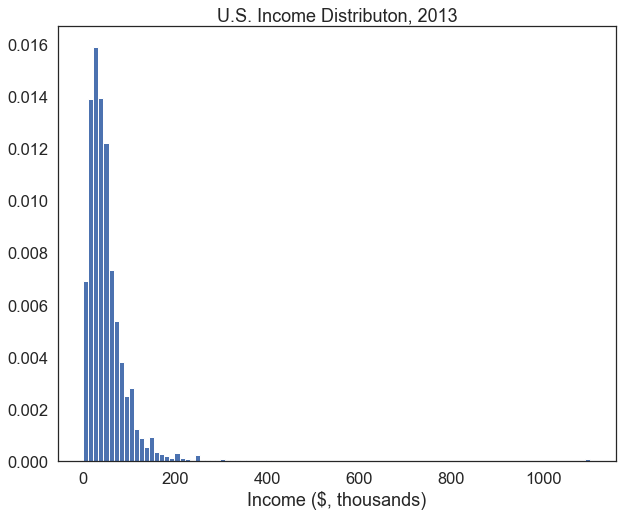
\includegraphics{notebooks/W05. Distributions and Basic Statistics_files/figure-pdf/cell-11-output-1.png}

}

\end{figure}

This is a pretty ugly histogram, and it's not telling us very much
useful information. It shows that the vast majority of people make
between 0 and \$100,000 per year, and a few make over 200k. A small
number make over \$1 million per year, so the plot is being extended to
accomodate these outliers. Let's try fixing the histogram up a bit.

\begin{Shaded}
\begin{Highlighting}[]
\NormalTok{plt.hist(df[}\StringTok{\textquotesingle{}income\textquotesingle{}}\NormalTok{], bins}\OperatorTok{=}\DecValTok{100}\NormalTok{, edgecolor}\OperatorTok{=}\StringTok{\textquotesingle{}white\textquotesingle{}}\NormalTok{, density}\OperatorTok{=}\VariableTok{True}\NormalTok{) }
\CommentTok{\# i\textquotesingle{}ve increased the number of bins to 100 to make the plot smoother,}
\CommentTok{\# added the density=True argument to make the y{-}axis a probability density instead of a count,}
\CommentTok{\# and the edgecolor=\textquotesingle{}white\textquotesingle{} argument to add some space between the bars, making the plot easier to read}


\NormalTok{plt.xlabel(}\StringTok{\textquotesingle{}Income ($, thousands)\textquotesingle{}}\NormalTok{) }\CommentTok{\# add a label to the x axis}
\NormalTok{plt.title(}\StringTok{"U.S. Income Distributon, 2013"}\NormalTok{) }\CommentTok{\# add a title to the plot}

\NormalTok{plt.show() }
\end{Highlighting}
\end{Shaded}

\begin{figure}[H]

{\centering \includegraphics{notebooks/W05. Distributions and Basic Statistics_files/figure-pdf/cell-12-output-1.png}

}

\end{figure}

That's better. We can now see more variation in how much people earn
within the \$0-200,000 range since we increased the number of bins in
the histogram. It could still be improved, though. The outliers making
over \$ 1 million are creating lots of dead space in this plot. We can
defensibly omit them from the plot, as long as we acknowledge that we've
done this somewhere in our analysis.

Let's also plot the mean and median of our distribution.

\begin{Shaded}
\begin{Highlighting}[]
\NormalTok{inc\_summary}\OperatorTok{=}\NormalTok{df[}\StringTok{\textquotesingle{}income\textquotesingle{}}\NormalTok{].describe() }\CommentTok{\# get summary statistics for the income variable using the describe() method, and store them in a variable called inc\_summary}
\BuiltInTok{print}\NormalTok{(inc\_summary[[}\StringTok{\textquotesingle{}mean\textquotesingle{}}\NormalTok{,}\StringTok{\textquotesingle{}50\%\textquotesingle{}}\NormalTok{,}\StringTok{\textquotesingle{}std\textquotesingle{}}\NormalTok{]]) }\CommentTok{\# print the mean, median and standard deviation}

\NormalTok{plt.hist(df[}\StringTok{\textquotesingle{}income\textquotesingle{}}\NormalTok{], bins}\OperatorTok{=}\DecValTok{100}\NormalTok{, edgecolor}\OperatorTok{=}\StringTok{\textquotesingle{}white\textquotesingle{}}\NormalTok{, density}\OperatorTok{=}\VariableTok{True}\NormalTok{) }\CommentTok{\# plot the histogram again}
\NormalTok{plt.axvline(inc\_summary[}\StringTok{\textquotesingle{}mean\textquotesingle{}}\NormalTok{], color}\OperatorTok{=}\StringTok{\textquotesingle{}red\textquotesingle{}}\NormalTok{, linestyle}\OperatorTok{=}\StringTok{\textquotesingle{}dashed\textquotesingle{}}\NormalTok{, linewidth}\OperatorTok{=}\DecValTok{1}\NormalTok{,label}\OperatorTok{=}\StringTok{\textquotesingle{}Mean\textquotesingle{}}\NormalTok{) }\CommentTok{\# get the mean from the inc\_summary variable and plot a vertical line in red at that point}
\NormalTok{plt.axvline(inc\_summary[}\StringTok{\textquotesingle{}50\%\textquotesingle{}}\NormalTok{], color}\OperatorTok{=}\StringTok{\textquotesingle{}black\textquotesingle{}}\NormalTok{, linestyle}\OperatorTok{=}\StringTok{\textquotesingle{}dashed\textquotesingle{}}\NormalTok{, linewidth}\OperatorTok{=}\DecValTok{1}\NormalTok{, label}\OperatorTok{=}\StringTok{\textquotesingle{}Median\textquotesingle{}}\NormalTok{) }\CommentTok{\# do the same for the median, but plot it in black}

\NormalTok{plt.legend()}
\NormalTok{plt.xlabel(}\StringTok{\textquotesingle{}Income ($, thousands\textquotesingle{}}\NormalTok{)}
\NormalTok{plt.title(}\StringTok{"U.S. Income Distributon, 2013"}\NormalTok{)}
\NormalTok{plt.xlim(}\DecValTok{0}\NormalTok{,}\DecValTok{250}\NormalTok{) }\CommentTok{\# set the x{-}axis limits to 0 to 250{-}{-} this will get rid of the outliers on the right side of the plot}

\NormalTok{plt.show()}
\end{Highlighting}
\end{Shaded}

\begin{verbatim}
mean    51.821863
50%     40.000000
std     60.163449
Name: income, dtype: float64
\end{verbatim}

\begin{figure}[H]

{\centering \includegraphics{notebooks/W05. Distributions and Basic Statistics_files/figure-pdf/cell-13-output-2.png}

}

\end{figure}

This histogram is far more informative-- use the questions in the
exercise below to guide your interpretation of this plot.

\hypertarget{exercise-12}{%
\subsection{Exercise}\label{exercise-12}}

\begin{enumerate}
\def\labelenumi{\arabic{enumi}.}
\tightlist
\item
  What is the (approximate) mean of this distribution?
\item
  What is the median?
\item
  Keeping in mind that we've excluded some extreme values, why might the
  mean be larger than the median? Intepret this qualitatively in
  reference to income inequality.
\item
  There are slight bumps in density at \$100,000, \$150,000, \$200,000,
  and \$250,000. Why might this be?
\end{enumerate}

As we have seen, there are a few extreme outliers in the income
distribution (really rich people). Outliers can bias some statistical
tests, so for the rest of this workbook, we're going to subset our
dataframe to exclude those who make over \$200k per year:

\begin{Shaded}
\begin{Highlighting}[]
\NormalTok{df}\OperatorTok{=}\NormalTok{df[df[}\StringTok{\textquotesingle{}income\textquotesingle{}}\NormalTok{]}\OperatorTok{\textless{}}\DecValTok{200}\NormalTok{]}
\end{Highlighting}
\end{Shaded}

\hypertarget{functions}{%
\section{Functions}\label{functions}}

Now we've got a pretty good sense of what's going on with the income
variable. But suppose we want to do this for another variable. We could
just copy and paste the code above, switch around the variable in
question, and edit the labels. But there's a far more efficient way of
doing things. In Python and most programming languages, you can write
your own \textbf{function}.

A function is a block of code that you can call on to do a specific
task. You can write your own functions, or you can use functions that
other people have written. Functions are useful because they allow you
to write code once, and then call on it whenever you need it. This is
much more efficient than writing the same code over and over again. You
can define a function by using the \texttt{def} keyword. For example, we
can define a function called \texttt{variable\_stats} that will
calculate the mean, median, and standard deviation of the variable tha
you specify.

\begin{Shaded}
\begin{Highlighting}[]
\KeywordTok{def}\NormalTok{ variable\_stats(variable): }\CommentTok{\# define a function called variable\_stats that takes a variable as an argument}
\NormalTok{    mean }\OperatorTok{=}\NormalTok{ variable.mean() }\CommentTok{\# calculate the mean of the variable}
\NormalTok{    median }\OperatorTok{=}\NormalTok{ variable.median() }\CommentTok{\# calculate the median of the variable}
\NormalTok{    std }\OperatorTok{=}\NormalTok{ variable.std() }\CommentTok{\# calculate the standard deviation of the variable}
    \BuiltInTok{print}\NormalTok{(}\StringTok{"Mean: "} \OperatorTok{+} \BuiltInTok{str}\NormalTok{(mean)) }\CommentTok{\# print the mean}
    \BuiltInTok{print}\NormalTok{(}\StringTok{"Median: "} \OperatorTok{+} \BuiltInTok{str}\NormalTok{(median)) }\CommentTok{\# print the median}
    \BuiltInTok{print}\NormalTok{(}\StringTok{"Standard deviation: "} \OperatorTok{+} \BuiltInTok{str}\NormalTok{(std)) }\CommentTok{\# print the standard deviation}
\end{Highlighting}
\end{Shaded}

\begin{Shaded}
\begin{Highlighting}[]
\CommentTok{\# We can then call on this function whenever we want to calculate these statistics. }

\NormalTok{variable\_stats(df[}\StringTok{\textquotesingle{}income\textquotesingle{}}\NormalTok{]) }
\end{Highlighting}
\end{Shaded}

\begin{verbatim}
Mean: 46.75408852483797
Median: 40.0
Standard deviation: 32.82190958000738
\end{verbatim}

Now, to calculate the same values for the age variable, we can simply
change which variable we feed the function:

\begin{Shaded}
\begin{Highlighting}[]
\NormalTok{variable\_stats(df[}\StringTok{\textquotesingle{}age\textquotesingle{}}\NormalTok{]) }
\end{Highlighting}
\end{Shaded}

\begin{verbatim}
Mean: 42.845076809704665
Median: 43.0
Standard deviation: 10.576333292267508
\end{verbatim}

We can write a more complex function to deal with plotting new
histograms for different variables, since most of the code we need to
plot a histogram won't change from one variable to the next. A few
things will change-- the variable that we're plotting, the title of the
graph, and the labels on the x and y axes, and perhaps the number of
bins. We can write a function called \texttt{plot\_histogram} that takes
these four things as arguments, and then plots a histogram. Then, we can
call on this function whenever we want to plot a histogram of a new
variable. Below is the same code we used to plot the histogram of
income, but this time we've written it as a function called
\texttt{plot\_histogram} and substituted the variable name
\texttt{income} for the argument \texttt{variable}.

\begin{Shaded}
\begin{Highlighting}[]
\KeywordTok{def}\NormalTok{ plot\_histogram(variable, bin\_number, xlab, title): }\CommentTok{\# define a function called plot\_histogram that takes a variable, number of bins, x{-}axis label, and title as arguments}
    
\NormalTok{    summary}\OperatorTok{=}\NormalTok{variable.describe()     }
\NormalTok{    plt.hist(variable, bins}\OperatorTok{=}\NormalTok{bin\_number,edgecolor}\OperatorTok{=}\StringTok{\textquotesingle{}white\textquotesingle{}}\NormalTok{, density}\OperatorTok{=}\VariableTok{True}\NormalTok{) }\CommentTok{\# plot the histogram. Notice i\textquotesingle{}ve changed "bins=100" to "bins=bin\_number" so that the number of bins can be specified when the function is called}
\NormalTok{    plt.axvline(summary[}\StringTok{\textquotesingle{}mean\textquotesingle{}}\NormalTok{], color}\OperatorTok{=}\StringTok{\textquotesingle{}red\textquotesingle{}}\NormalTok{, linestyle}\OperatorTok{=}\StringTok{\textquotesingle{}dashed\textquotesingle{}}\NormalTok{, linewidth}\OperatorTok{=}\DecValTok{1}\NormalTok{,label}\OperatorTok{=}\StringTok{\textquotesingle{}Mean \textquotesingle{}}\OperatorTok{+}\BuiltInTok{str}\NormalTok{(}\BuiltInTok{round}\NormalTok{(summary[}\StringTok{\textquotesingle{}mean\textquotesingle{}}\NormalTok{],}\DecValTok{2}\NormalTok{)))}
\NormalTok{    plt.axvline(summary[}\StringTok{\textquotesingle{}50\%\textquotesingle{}}\NormalTok{], color}\OperatorTok{=}\StringTok{\textquotesingle{}black\textquotesingle{}}\NormalTok{, linestyle}\OperatorTok{=}\StringTok{\textquotesingle{}dashed\textquotesingle{}}\NormalTok{, linewidth}\OperatorTok{=}\DecValTok{1}\NormalTok{, label}\OperatorTok{=}\StringTok{\textquotesingle{}Median \textquotesingle{}}\OperatorTok{+}\BuiltInTok{str}\NormalTok{(}\BuiltInTok{round}\NormalTok{(summary[}\StringTok{\textquotesingle{}50\%\textquotesingle{}}\NormalTok{],}\DecValTok{2}\NormalTok{)))}

\NormalTok{    plt.legend()}
\NormalTok{    plt.xlabel(xlab) }\CommentTok{\# i\textquotesingle{}ve changed the x{-}axis label to "xlab" so that it can be specified when the function is called}
\NormalTok{    plt.title(title) }\CommentTok{\# similarly, we can now specify the title when calling the function}
\NormalTok{    plt.show()}
\end{Highlighting}
\end{Shaded}

Now we can just call the function with the variable we want to plot, the
number of bins, the x-axis label, and the title using one line of code.
Let's recreate the histogram of income from above, but this time using
the function we just defined:

\begin{Shaded}
\begin{Highlighting}[]
\NormalTok{plot\_histogram(variable }\OperatorTok{=}\NormalTok{ df[}\StringTok{\textquotesingle{}income\textquotesingle{}}\NormalTok{], bin\_number }\OperatorTok{=} \DecValTok{20}\NormalTok{, xlab }\OperatorTok{=} \StringTok{\textquotesingle{}Income ($, 000)\textquotesingle{}}\NormalTok{, title }\OperatorTok{=} \StringTok{\textquotesingle{}U.S. Income Distribution, 2013\textquotesingle{}}\NormalTok{)}
\end{Highlighting}
\end{Shaded}

\begin{figure}[H]

{\centering \includegraphics{notebooks/W05. Distributions and Basic Statistics_files/figure-pdf/cell-19-output-1.png}

}

\end{figure}

If we want to produce lots of similar plots, this really helps us cut
down on repetition.

\hypertarget{exercise-13}{%
\subsection{Exercise}\label{exercise-13}}

\begin{enumerate}
\def\labelenumi{\arabic{enumi}.}
\tightlist
\item
  Plot the histogram of the `age' variable with 80 bins, label the
  x-axis ``Age'', and add title of `U.S. Age Distribution, 2013'.
\item
  Plot the distribution of schooling years.

  \begin{itemize}
  \tightlist
  \item
    Find an appropriate number of bins
  \item
    Label it clearly
  \item
    Interpret salient trends
  \end{itemize}
\end{enumerate}

\hypertarget{the-central-limit-theorem}{%
\section{The Central Limit Theorem}\label{the-central-limit-theorem}}

But as we learned in class, the Central Limit Theorem states that the
\textbf{distribution of the mean of a sample of observations will be
approximately normal, regardless of the distribution of the original
observations}. So, if we take a \textbf{large enough sample} of
observations from each of these variables, and calculate the mean of
each sample, we should get a normal distribution. This is important
because the normal distribution behaves in a very predictable way.

The code below creates a ``standard normal'' distribution with a mean of
0 and a standard deviation of 1:

\begin{Shaded}
\begin{Highlighting}[]
\NormalTok{mu, se}\OperatorTok{=} \DecValTok{0}\NormalTok{, }\DecValTok{1} \CommentTok{\# create two variables, a mean "mu" equal to zero, and standard deviation "se" equal to 1}
\NormalTok{x }\OperatorTok{=}\NormalTok{ np.linspace(mu }\OperatorTok{{-}} \DecValTok{3}\OperatorTok{*}\NormalTok{se, mu }\OperatorTok{+} \DecValTok{3}\OperatorTok{*}\NormalTok{se, }\DecValTok{100}\NormalTok{) }\CommentTok{\# create a range of values from {-}3 to 3 standard deviations}

\NormalTok{plt.plot(x, norm.pdf(x, mu, se)) }\CommentTok{\# plot the normal distribution}
\NormalTok{plt.axvline(mu, color}\OperatorTok{=}\StringTok{\textquotesingle{}black\textquotesingle{}}\NormalTok{, linestyle}\OperatorTok{=}\StringTok{\textquotesingle{}solid\textquotesingle{}}\NormalTok{, linewidth}\OperatorTok{=}\DecValTok{1}\NormalTok{,label}\OperatorTok{=}\StringTok{\textquotesingle{}µ\textquotesingle{}}\NormalTok{)  }\CommentTok{\# plot a vertical line at the mean}
\NormalTok{plt.axvline(mu}\OperatorTok{{-}}\NormalTok{se}\OperatorTok{*}\DecValTok{2}\NormalTok{, color}\OperatorTok{=}\StringTok{\textquotesingle{}black\textquotesingle{}}\NormalTok{, linestyle}\OperatorTok{=}\StringTok{\textquotesingle{}dashed\textquotesingle{}}\NormalTok{, linewidth}\OperatorTok{=}\FloatTok{1.5}\NormalTok{,label}\OperatorTok{=}\StringTok{\textquotesingle{}µ ± 2σ\textquotesingle{}}\NormalTok{) }\CommentTok{\# plot a vertical line at the mean plus 2 standard deviations}
\NormalTok{plt.axvline(mu}\OperatorTok{+}\NormalTok{se}\OperatorTok{*}\DecValTok{2}\NormalTok{, color}\OperatorTok{=}\StringTok{\textquotesingle{}black\textquotesingle{}}\NormalTok{, linestyle}\OperatorTok{=}\StringTok{\textquotesingle{}dashed\textquotesingle{}}\NormalTok{, linewidth}\OperatorTok{=}\FloatTok{1.5}\NormalTok{)  }\CommentTok{\# plot a vertical line at the mean minus 2 standard deviations}
\NormalTok{plt.legend()}
\NormalTok{plt.show()}
\end{Highlighting}
\end{Shaded}

\begin{figure}[H]

{\centering 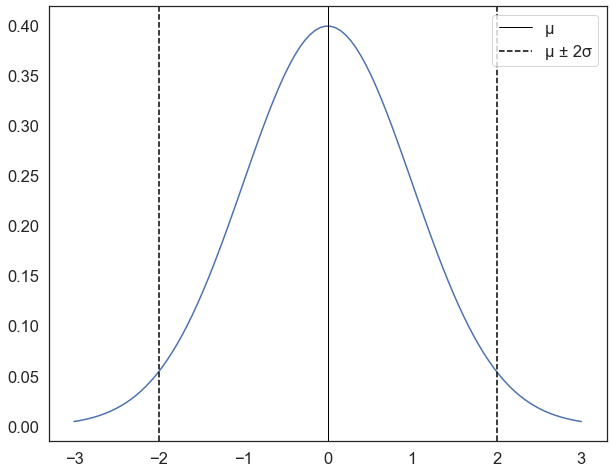
\includegraphics{notebooks/W05. Distributions and Basic Statistics_files/figure-pdf/cell-22-output-1.png}

}

\end{figure}

for a distribution with this shape,

\begin{verbatim}
* 68% of the values will be within 1 standard deviation of the mean
* 95.45% of the values will be within 2 standard deviations of the mean
* 99.7% of the values will be within 3 standard deviations of the mean
\end{verbatim}

so in the plot above, if I took a random value from the distribution,
there's a 95\% chance that it would be between -2 and 2 (within the
dotted lines), and a 99.7\% chance that it would be between -3 and 3.

It's crucial to note, however, that this applies to the mean of a
sample, not individual observations. For example, this doesnt mean that
there is a 95\% chance that an individual taken at random will have an
income that is within 2 standard deviations of the mean (\$46k). It
means that if we take a sample of 100 observations, there is a 95\%
chance that the \textbf{mean of that sample} will be within 2 standard
deviations of the mean (\$46k).

\hypertarget{sampling}{%
\subsection{Sampling}\label{sampling}}

To illustrate how this works, for the rest of this workshop we're going
to pretend that the dataframe contains the entire adult
\textbf{population} of the United States (of course, it is actually a
sample but just pretend). The mean of this distribution will thus be the
\textbf{population mean}; for the income variable, this is \$46k.

We can use the \texttt{sample} function to take a random sample of
observations from a distribution. We'll take a sample of 5 observations
from the income variable and use the \texttt{mean} function to calculate
the mean of this sample.

\begin{Shaded}
\begin{Highlighting}[]
\NormalTok{income\_sample }\OperatorTok{=}\NormalTok{ df[}\StringTok{\textquotesingle{}income\textquotesingle{}}\NormalTok{].sample(}\DecValTok{5}\NormalTok{, replace}\OperatorTok{=}\VariableTok{True}\NormalTok{) }\CommentTok{\# take a random sample of 10 observations from the income variable}
\NormalTok{income\_sample\_mean}\OperatorTok{=}\NormalTok{income\_sample.mean() }\CommentTok{\# calculate the mean of the sample}
\BuiltInTok{print}\NormalTok{(}\StringTok{"Mean: "} \OperatorTok{+} \BuiltInTok{str}\NormalTok{(income\_sample\_mean)) }\CommentTok{\# print the sample mean}
\end{Highlighting}
\end{Shaded}

\begin{verbatim}
Mean: 33.0
\end{verbatim}

\hypertarget{exercise-14}{%
\subsection{Exercise}\label{exercise-14}}

\begin{enumerate}
\def\labelenumi{\arabic{enumi}.}
\tightlist
\item
  Run the code cell above 10 times and make note of the mean. What is
  the farthest the sample mean deviates from the ``population'' mean of
  \$51k?
\item
  Increase the sample size from 5 to 100 and run the cell 10 more times.
  Now, what is the farthest the sample mean deviates from the population
  mean?
\item
  Increase the sample size to 1000. What do you notice about the sample
  means as we increase the sample size?
\end{enumerate}

Hopefully, you will have noticed that as the sample size increases, the
sample means tend to be closer to the population mean. But clicking that
cell is hard work. Let's create a loop that will run that block of code
10000 times, save the sample means in a list, and plot the distribution
of sample means as a histogram. Once again, we'll start by only drawing
samples of 10 observations:

\begin{Shaded}
\begin{Highlighting}[]
\CommentTok{\#create an empty list to store sample means}
\NormalTok{sample\_means}\OperatorTok{=}\NormalTok{[]}

\NormalTok{sample\_size}\OperatorTok{=}\DecValTok{10}
\CommentTok{\# loop 10,000 times.}
\ControlFlowTok{for}\NormalTok{ i }\KeywordTok{in} \BuiltInTok{range}\NormalTok{(}\DecValTok{0}\NormalTok{,}\DecValTok{10000}\NormalTok{):}
\NormalTok{    sample}\OperatorTok{=}\NormalTok{ df[}\StringTok{\textquotesingle{}income\textquotesingle{}}\NormalTok{].sample(sample\_size, replace}\OperatorTok{=}\VariableTok{True}\NormalTok{) }\CommentTok{\# draw a sample of 10 observations from the income variable, with replacement}
\NormalTok{    sample\_mean}\OperatorTok{=}\NormalTok{sample.mean() }\CommentTok{\# calculate the mean of the sample}
\NormalTok{    sample\_means.append(sample\_mean) }\CommentTok{\# append the sample mean to the list of sample means}
    
\NormalTok{plt.hist(sample\_means, bins}\OperatorTok{=}\DecValTok{30}\NormalTok{, edgecolor}\OperatorTok{=}\StringTok{\textquotesingle{}white\textquotesingle{}}\NormalTok{, density}\OperatorTok{=}\VariableTok{True}\NormalTok{) }\CommentTok{\# plot a histogram of the sample means}
\NormalTok{plt.title(}\StringTok{\textquotesingle{}Distribution of Sample Means (n=}\SpecialCharTok{\{\}}\StringTok{)\textquotesingle{}}\NormalTok{.}\BuiltInTok{format}\NormalTok{(sample\_size)) }\CommentTok{\# add a title}
\NormalTok{plt.show()}
\end{Highlighting}
\end{Shaded}

\begin{figure}[H]

{\centering 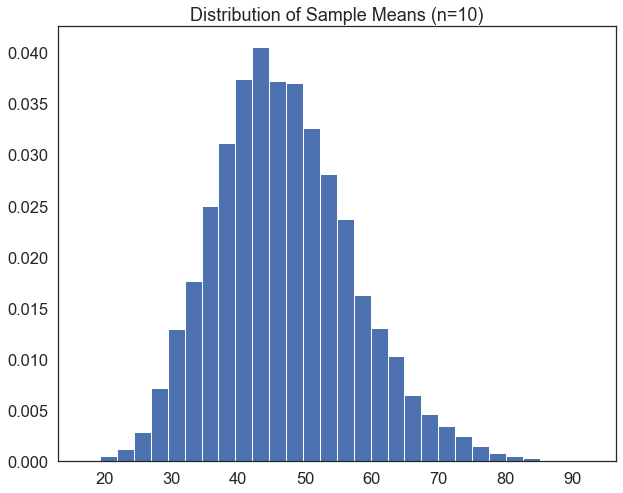
\includegraphics{notebooks/W05. Distributions and Basic Statistics_files/figure-pdf/cell-24-output-1.png}

}

\end{figure}

\hypertarget{exercise-15}{%
\subsection{Exercise}\label{exercise-15}}

\begin{verbatim}
1. Edit the code block above so that instead of drawing samples of 10 observations, it draws samples of 1000 observations
2. What happens to the distribution?
\end{verbatim}

When we draw 10,000 samples of 1000 observations each, the distribution
of sample means looks a lot more normally distributed than the
underlying distribution of income itself, which is skewed to the right.
To show how normally distributed it is, let's overlay the normal
distribution line we plotted earlier and fit it to the distribution of
sample means. We'll start off by making the same histogram of sample
means, but add a line plot of the normal distribution and some droplines
at ± 2 standard deviations.

Because we may want to do this for several different variables, let's
once again package our code as a function in which we can swap around a
couple bits. In this case, we may want to swap around the variable we're
plotting, the label on the x-axis, and the size of the samples we're
drawing. So we'll create a function called \texttt{plot\_sample\_means}
that takes these three things as arguments (\texttt{var}, \texttt{xlab},
and \texttt{sample\_size}).

\begin{Shaded}
\begin{Highlighting}[]
\KeywordTok{def}\NormalTok{ plot\_sample\_means(var, xlab, sample\_size): }\CommentTok{\# define a function called plot\_sample\_means that takes a variable, x{-}axis label, and sample size as arguments}

    \CommentTok{\#create an empty list to store sample means}
\NormalTok{    sample\_means}\OperatorTok{=}\NormalTok{[]}

    \CommentTok{\# loop 10,000 times.}
    \ControlFlowTok{for}\NormalTok{ i }\KeywordTok{in} \BuiltInTok{range}\NormalTok{(}\DecValTok{0}\NormalTok{,}\DecValTok{10000}\NormalTok{):}
        \CommentTok{\# for each iteration, draw a sample of the size specified by the "sample\_size" parameter}
\NormalTok{        sample}\OperatorTok{=}\NormalTok{var.sample(sample\_size, replace}\OperatorTok{=}\VariableTok{True}\NormalTok{)}
        \CommentTok{\# calculate the mean, and append it to the list of sample means. }
\NormalTok{        sample\_mean}\OperatorTok{=}\NormalTok{sample.mean()}
\NormalTok{        sample\_means.append(sample\_mean)}
    
    \CommentTok{\# now, plot a histogram }
\NormalTok{    plt.hist(sample\_means, color}\OperatorTok{=}\StringTok{\textquotesingle{}blue\textquotesingle{}}\NormalTok{,alpha}\OperatorTok{=}\FloatTok{0.5}\NormalTok{, bins}\OperatorTok{=}\BuiltInTok{int}\NormalTok{(}\DecValTok{30}\NormalTok{), edgecolor}\OperatorTok{=}\StringTok{\textquotesingle{}white\textquotesingle{}}\NormalTok{, density}\OperatorTok{=}\VariableTok{True}\NormalTok{)}
    
    \CommentTok{\# fit a normal distribution to the data }
\NormalTok{    mu, se }\OperatorTok{=}\NormalTok{ norm.fit(sample\_means)}
\NormalTok{    xmin, xmax }\OperatorTok{=}\NormalTok{ plt.xlim()}
\NormalTok{    x }\OperatorTok{=}\NormalTok{ np.linspace(xmin, xmax, }\DecValTok{100}\NormalTok{)}
\NormalTok{    p }\OperatorTok{=}\NormalTok{ norm.pdf(x, mu, se) }
\NormalTok{    plt.plot(x, p, }\StringTok{\textquotesingle{}k\textquotesingle{}}\NormalTok{, linewidth}\OperatorTok{=}\DecValTok{2}\NormalTok{)}

    \CommentTok{\# calculate the difference between the mean of the sample means }
\NormalTok{    diff}\OperatorTok{=}\BuiltInTok{abs}\NormalTok{(mu}\OperatorTok{{-}}\NormalTok{var.mean())}
    
    \CommentTok{\# add droplines, labels, title, legend, and limit the x{-}axis range to 3 standard deviations from the mean on either side.}
\NormalTok{    plt.axvline(mu, color}\OperatorTok{=}\StringTok{\textquotesingle{}green\textquotesingle{}}\NormalTok{, linestyle}\OperatorTok{=}\StringTok{\textquotesingle{}solid\textquotesingle{}}\NormalTok{, linewidth}\OperatorTok{=}\DecValTok{3}\NormalTok{,label}\OperatorTok{=}\StringTok{\textquotesingle{}µx̄=\textquotesingle{}}\OperatorTok{+}\BuiltInTok{str}\NormalTok{(}\BuiltInTok{round}\NormalTok{(mu, }\DecValTok{3}\NormalTok{)))}
\NormalTok{    plt.axvline(mu}\OperatorTok{{-}}\NormalTok{se}\OperatorTok{*}\DecValTok{2}\NormalTok{, color}\OperatorTok{=}\StringTok{\textquotesingle{}black\textquotesingle{}}\NormalTok{, linestyle}\OperatorTok{=}\StringTok{\textquotesingle{}dashed\textquotesingle{}}\NormalTok{, linewidth}\OperatorTok{=}\FloatTok{1.5}\NormalTok{,label}\OperatorTok{=}\StringTok{\textquotesingle{}µ ± 2σ\textquotesingle{}}\NormalTok{)}
\NormalTok{    plt.axvline(mu}\OperatorTok{+}\NormalTok{se}\OperatorTok{*}\DecValTok{2}\NormalTok{, color}\OperatorTok{=}\StringTok{\textquotesingle{}black\textquotesingle{}}\NormalTok{, linestyle}\OperatorTok{=}\StringTok{\textquotesingle{}dashed\textquotesingle{}}\NormalTok{, linewidth}\OperatorTok{=}\FloatTok{1.5}\NormalTok{)}
\NormalTok{    plt.legend()}
\NormalTok{    plt.xlabel(xlab)    }
\NormalTok{    plt.title(}\StringTok{\textquotesingle{}Distribution of Sample Means (n=}\SpecialCharTok{\{\}}\StringTok{)\textquotesingle{}}\NormalTok{.}\BuiltInTok{format}\NormalTok{(sample\_size))}
\NormalTok{    plt.xlim(mu}\OperatorTok{{-}}\NormalTok{se}\OperatorTok{*}\DecValTok{3}\NormalTok{, mu}\OperatorTok{+}\NormalTok{se}\OperatorTok{*}\DecValTok{3}\NormalTok{)}
\NormalTok{    plt.show()  }
\end{Highlighting}
\end{Shaded}

\begin{Shaded}
\begin{Highlighting}[]
\NormalTok{plot\_sample\_means(df[}\StringTok{\textquotesingle{}income\textquotesingle{}}\NormalTok{], xlab}\OperatorTok{=}\StringTok{\textquotesingle{}Income, ($, 000)\textquotesingle{}}\NormalTok{, sample\_size}\OperatorTok{=}\DecValTok{1000}\NormalTok{)}
\end{Highlighting}
\end{Shaded}

\begin{figure}[H]

{\centering 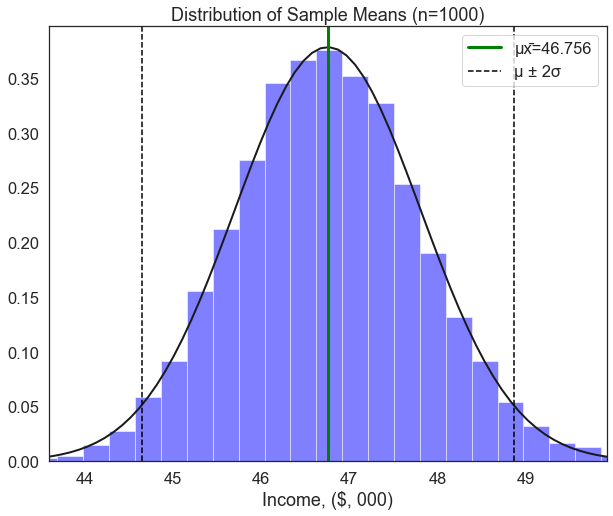
\includegraphics{notebooks/W05. Distributions and Basic Statistics_files/figure-pdf/cell-26-output-1.png}

}

\end{figure}

We can see that the distribution of sample means (for samples of 1000
people) very closely approximates the normal distribution. The addition
of droplines at ±2σ tells us that \textbf{if we take a random sample of
1000 people, there is a 95\% chance that the mean of this sample will
fall between \textasciitilde\$44.7k and \textasciitilde\$48.8k}.

Why is this important? let's see what happens when we filter the sample
based on peoples' attributes. The code below creates two dataframes: one
called \texttt{men} which only contains male respondents, and one called
\texttt{women} which only contains female respondents. Then, we run the
\texttt{plot\_sample\_means()} function on each of these dataframes.

\begin{Shaded}
\begin{Highlighting}[]
\NormalTok{men}\OperatorTok{=}\NormalTok{df[df[}\StringTok{\textquotesingle{}sex\textquotesingle{}}\NormalTok{]}\OperatorTok{==}\DecValTok{1}\NormalTok{][}\StringTok{\textquotesingle{}income\textquotesingle{}}\NormalTok{] }\CommentTok{\# create a new dataframe containing only income values for men}
\NormalTok{women}\OperatorTok{=}\NormalTok{df[df[}\StringTok{\textquotesingle{}sex\textquotesingle{}}\NormalTok{]}\OperatorTok{==}\DecValTok{2}\NormalTok{][}\StringTok{\textquotesingle{}income\textquotesingle{}}\NormalTok{] }\CommentTok{\# create a new dataframe containing only income values for women}

\NormalTok{plot\_sample\_means(men, xlab}\OperatorTok{=}\StringTok{\textquotesingle{}Income, ($, 000)\textquotesingle{}}\NormalTok{, sample\_size}\OperatorTok{=}\DecValTok{500}\NormalTok{)}
\NormalTok{plot\_sample\_means(women, xlab}\OperatorTok{=}\StringTok{\textquotesingle{}Income, ($, 000)\textquotesingle{}}\NormalTok{, sample\_size}\OperatorTok{=}\DecValTok{500}\NormalTok{)}
\end{Highlighting}
\end{Shaded}

\begin{figure}[H]

{\centering 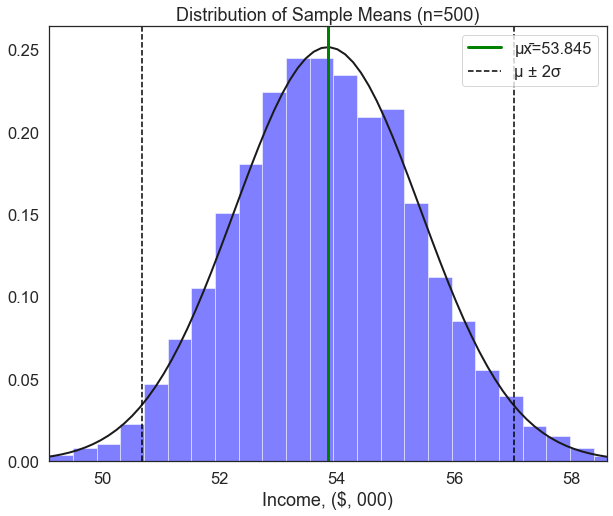
\includegraphics{notebooks/W05. Distributions and Basic Statistics_files/figure-pdf/cell-27-output-1.png}

}

\end{figure}

\begin{figure}[H]

{\centering 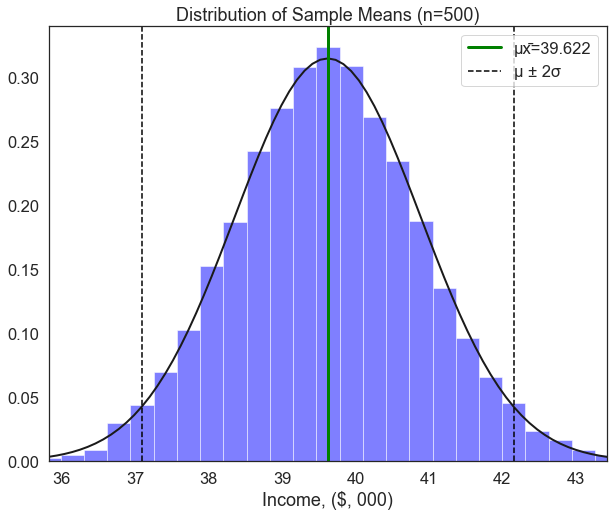
\includegraphics{notebooks/W05. Distributions and Basic Statistics_files/figure-pdf/cell-27-output-2.png}

}

\end{figure}

\hypertarget{exercise-16}{%
\subsection{Exercise}\label{exercise-16}}

\begin{verbatim}
1. These two histograms may look the same, but look closely at the values. 
2. The population mean income for women is around $39.6k. Based on the histogram of sample means taken from only men, 
    * What is the likelihood of observing a sample mean of $39.6k among men due to random chance?
3. Interpret this finding qualitatively.
\end{verbatim}

The plot of incomes for men and women show very different distributions,
but they look quite similar. To make this more readable, let's define
one last function that can take two or more groups and plot the
distribution of their sample means on the same plot:

\begin{Shaded}
\begin{Highlighting}[]
\KeywordTok{def}\NormalTok{ two\_hist(groups,group\_labs,xlab, title): }\CommentTok{\# define a function called two\_hist that takes a list of groups, a list of group labels, an x{-}axis label, and a title as arguments}

\NormalTok{        plt.figure(figsize}\OperatorTok{=}\NormalTok{(}\DecValTok{15}\NormalTok{,}\DecValTok{6}\NormalTok{)) }\CommentTok{\# set the figure size}

\NormalTok{        it}\OperatorTok{={-}}\DecValTok{1} \CommentTok{\# create a counter variable called "it" and set it equal to {-}1}
        \ControlFlowTok{for}\NormalTok{ var }\KeywordTok{in}\NormalTok{ groups: }\CommentTok{\# loop through each group in the list of groups}
\NormalTok{            it}\OperatorTok{+=}\DecValTok{1} \CommentTok{\# increase the iterator by 1}
\NormalTok{            sample\_size}\OperatorTok{=}\DecValTok{1000} \CommentTok{\# set the sample size equal to 1000}
\NormalTok{            sample\_means}\OperatorTok{=}\NormalTok{[] }\CommentTok{\# create an empty list to store sample means}
\NormalTok{            iterations}\OperatorTok{=}\DecValTok{10000} \CommentTok{\# set the number of iterations equal to 10,000}

            \ControlFlowTok{for}\NormalTok{ i }\KeywordTok{in} \BuiltInTok{range}\NormalTok{(}\DecValTok{0}\NormalTok{,iterations): }\CommentTok{\# loop through the number of iterations}
\NormalTok{                sample}\OperatorTok{=}\NormalTok{var.sample(sample\_size, replace}\OperatorTok{=}\VariableTok{True}\NormalTok{) }\CommentTok{\# draw a sample of the size specified by the "sample\_size" parameter}
\NormalTok{                sample\_mean}\OperatorTok{=}\NormalTok{sample.mean() }\CommentTok{\# calculate the mean of the sample}
\NormalTok{                sample\_means.append(sample\_mean) }\CommentTok{\# append the sample mean to the list of sample means}
            
\NormalTok{            plt.hist(sample\_means, bins}\OperatorTok{=}\BuiltInTok{int}\NormalTok{(iterations}\OperatorTok{/}\DecValTok{300}\NormalTok{),edgecolor}\OperatorTok{=}\StringTok{\textquotesingle{}white\textquotesingle{}}\NormalTok{,density}\OperatorTok{=}\VariableTok{True}\NormalTok{, label}\OperatorTok{=}\NormalTok{group\_labs[it])  }\CommentTok{\# plot a histogram of the sample means}
\NormalTok{            mu, se }\OperatorTok{=}\NormalTok{ norm.fit(sample\_means) }\CommentTok{\# fit a normal distribution to the data}
\NormalTok{            xmin, xmax }\OperatorTok{=}\NormalTok{ plt.xlim() }\CommentTok{\# set the x{-}axis limits}
\NormalTok{            x }\OperatorTok{=}\NormalTok{ np.linspace(xmin, xmax, }\DecValTok{100}\NormalTok{) }\CommentTok{\# create a range of values from the minimum to the maximum x{-}axis value}
\NormalTok{            p }\OperatorTok{=}\NormalTok{ norm.pdf(x, mu, se) }\CommentTok{\# calculate the probability density function for the normal distribution}

\NormalTok{            plt.plot(x, p, }\StringTok{\textquotesingle{}k\textquotesingle{}}\NormalTok{, linewidth}\OperatorTok{=}\DecValTok{2}\NormalTok{) }\CommentTok{\# plot the normal distribution}
\NormalTok{            plt.xlabel(xlab) }\CommentTok{\# add an x{-}axis label}
\NormalTok{            plt.title(title) }\CommentTok{\# add a title}
\NormalTok{            plt.axvline(var.mean(), color}\OperatorTok{=}\StringTok{\textquotesingle{}green\textquotesingle{}}\NormalTok{, linestyle}\OperatorTok{=}\StringTok{\textquotesingle{}solid\textquotesingle{}}\NormalTok{, linewidth}\OperatorTok{=}\DecValTok{3}\NormalTok{) }\CommentTok{\# add a vertical line at the mean of the variable}
\NormalTok{            plt.axvline(mu}\OperatorTok{{-}}\NormalTok{se}\OperatorTok{*}\DecValTok{2}\NormalTok{, color}\OperatorTok{=}\StringTok{\textquotesingle{}black\textquotesingle{}}\NormalTok{, linestyle}\OperatorTok{=}\StringTok{\textquotesingle{}dashed\textquotesingle{}}\NormalTok{, linewidth}\OperatorTok{=}\FloatTok{1.5}\NormalTok{)}
\NormalTok{            plt.axvline(mu}\OperatorTok{+}\NormalTok{se}\OperatorTok{*}\DecValTok{2}\NormalTok{, color}\OperatorTok{=}\StringTok{\textquotesingle{}black\textquotesingle{}}\NormalTok{, linestyle}\OperatorTok{=}\StringTok{\textquotesingle{}dashed\textquotesingle{}}\NormalTok{, linewidth}\OperatorTok{=}\FloatTok{1.5}\NormalTok{)}
\NormalTok{            plt.legend() }\CommentTok{\# add a legend}
            
\NormalTok{        plt.show()  }\CommentTok{\# show the plot }
\end{Highlighting}
\end{Shaded}

\begin{Shaded}
\begin{Highlighting}[]
\NormalTok{two\_hist([men,women],[}\StringTok{\textquotesingle{}Men\textquotesingle{}}\NormalTok{,}\StringTok{\textquotesingle{}Women\textquotesingle{}}\NormalTok{],}\StringTok{\textquotesingle{}Income ($, thousands)\textquotesingle{}}\NormalTok{, }\StringTok{"Income Sample Means"}\NormalTok{)}
\end{Highlighting}
\end{Shaded}

\begin{figure}[H]

{\centering 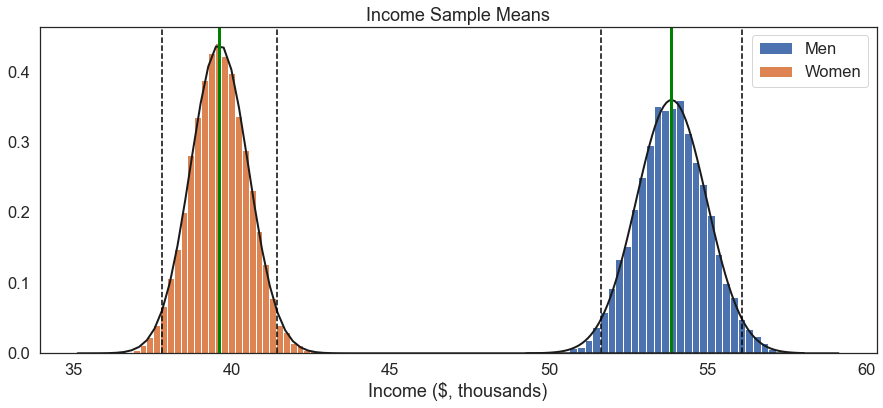
\includegraphics{notebooks/W05. Distributions and Basic Statistics_files/figure-pdf/cell-29-output-1.png}

}

\end{figure}

There we have it: A stark, quantitative representation of the gender
wage gap.

If we simply compared the means between a sample of women and a sample
of men, the best we could do in terms of inference would be to say
something like ``the average income for men was \$14.2k higher than it
was for women.'' Though this is an important finding, the central limit
theorem lets us add important context.

\begin{verbatim}
1. We took 10,000 large samples of men and calculated the means of each sample.
2. We found that over 99.7% of them were greater than $50,000. 
3. We took 10,000 large samples of women and calculated the means of each sample.
4. We found that over 99.7% of them were smaller than $44,000.
\end{verbatim}

The fact that the distribution of income sample means between men and
women do not overlap at all tells us that the probability of this
variation in incomes being due to random chance is extremely, extremely
small. Thus, we can say that the observed difference in income between
men and women is \textbf{statistically significant}.

\bookmarksetup{startatroot}

\hypertarget{merging-and-joining}{%
\chapter{Merging and Joining}\label{merging-and-joining}}

\hypertarget{reading-week-open-in-colab}{%
\section[\emph{Reading Week} ]{\texorpdfstring{\emph{Reading Week}
\href{https://colab.research.google.com/github/oballinger/QM2/blob/main/notebooks/RW.\%20Merging\%20and\%20Joining.ipynb}{\protect
\includegraphics{index_files/mediabag/colab-badge.png}}}{Reading Week Open In Colab}}\label{reading-week-open-in-colab}}

Sometimes, we will want to combine data from different sources about the
same subject - perhaps we want to compare the GDP in a country with life
expectancy, or the proportion of free schools meals with the level of
unemployment.

\hypertarget{aims-3}{%
\subsection{Aims}\label{aims-3}}

\begin{itemize}
\tightlist
\item
  Understand joins
\item
  Work with joining dataframes in Pandas
\item
  Create your own examples
\end{itemize}

\hypertarget{downloading-the-data-2}{%
\section{Downloading the Data}\label{downloading-the-data-2}}

Let's grab the data we will need this week from our course website and
save it into our data folder. If you've not already created a data
folder then do so using the following command.

Don't worry if it generates an error, that means you've already got a
data folder.

\begin{Shaded}
\begin{Highlighting}[]
\OperatorTok{!}\NormalTok{mkdir data}
\end{Highlighting}
\end{Shaded}

\begin{verbatim}
mkdir: cannot create directory ‘data’: File exists
\end{verbatim}

\begin{Shaded}
\begin{Highlighting}[]
\OperatorTok{!}\NormalTok{mkdir data}\OperatorTok{/}\NormalTok{wk5}
\OperatorTok{!}\NormalTok{curl https:}\OperatorTok{//}\NormalTok{s3.eu}\OperatorTok{{-}}\NormalTok{west}\OperatorTok{{-}}\FloatTok{2.}\ErrorTok{amazonaws}\NormalTok{.com}\OperatorTok{/}\NormalTok{qm2}\OperatorTok{/}\NormalTok{wk3}\OperatorTok{/}\NormalTok{UN\_Life\_all.csv }\OperatorTok{{-}}\NormalTok{o .}\OperatorTok{/}\NormalTok{data}\OperatorTok{/}\NormalTok{wk5}\OperatorTok{/}\NormalTok{UN\_Life\_all.csv}
\OperatorTok{!}\NormalTok{curl https:}\OperatorTok{//}\NormalTok{s3.eu}\OperatorTok{{-}}\NormalTok{west}\OperatorTok{{-}}\FloatTok{2.}\ErrorTok{amazonaws}\NormalTok{.com}\OperatorTok{/}\NormalTok{qm2}\OperatorTok{/}\NormalTok{wk3}\OperatorTok{/}\NormalTok{UN\_Cities\_1214\_country.csv }\OperatorTok{{-}}\NormalTok{o .}\OperatorTok{/}\NormalTok{data}\OperatorTok{/}\NormalTok{wk5}\OperatorTok{/}\NormalTok{UN\_Cities\_1214\_country.csv}
\OperatorTok{!}\NormalTok{curl https:}\OperatorTok{//}\NormalTok{s3.eu}\OperatorTok{{-}}\NormalTok{west}\OperatorTok{{-}}\FloatTok{2.}\ErrorTok{amazonaws}\NormalTok{.com}\OperatorTok{/}\NormalTok{qm2}\OperatorTok{/}\NormalTok{wk3}\OperatorTok{/}\NormalTok{UN\_Cities\_1214\_population.csv }\OperatorTok{{-}}\NormalTok{o .}\OperatorTok{/}\NormalTok{data}\OperatorTok{/}\NormalTok{wk5}\OperatorTok{/}\NormalTok{UN\_Cities\_1214\_population.csv}
\end{Highlighting}
\end{Shaded}

\begin{verbatim}
  % Total    % Received % Xferd  Average Speed   Time    Time     Time  Current
                                 Dload  Upload   Total   Spent    Left  Speed
100  354k  100  354k    0     0   411k      0 --:--:-- --:--:-- --:--:--  410k
  % Total    % Received % Xferd  Average Speed   Time    Time     Time  Current
                                 Dload  Upload   Total   Spent    Left  Speed
100 31445  100 31445    0     0  63397      0 --:--:-- --:--:-- --:--:-- 63397
  % Total    % Received % Xferd  Average Speed   Time    Time     Time  Current
                                 Dload  Upload   Total   Spent    Left  Speed
100  373k  100  373k    0     0   471k      0 --:--:-- --:--:-- --:--:--  471k
\end{verbatim}

\hypertarget{joining-instructions}{%
\section{Joining Instructions}\label{joining-instructions}}

Joins are the combination of different datasets, and are common in
relational databases as a way of performing queries. There are lots of
examples of why and when we might want to do this, but most start with
two tables of data. We're going to start with some data we've generated.

I'm going to go back and work with fake data for a while, because it's
clean and small and we can see what's going on - when we work with real
data, we have to take great care that the data is clean, the indices
match, and so on.

\begin{Shaded}
\begin{Highlighting}[]
\ImportTok{import}\NormalTok{ matplotlib.pyplot }\ImportTok{as}\NormalTok{ plt}
\ImportTok{import}\NormalTok{ pandas }\ImportTok{as}\NormalTok{ pd}
\ImportTok{import}\NormalTok{ numpy }\ImportTok{as}\NormalTok{ np}
\ImportTok{import}\NormalTok{ random}
\OperatorTok{\%}\NormalTok{matplotlib inline}
\end{Highlighting}
\end{Shaded}

Let's create dataframes which represent fictitious values associated
with people. Let's assume our data is anonymised because we're ethical
researchers and don't want information about real people leaking out.

\begin{Shaded}
\begin{Highlighting}[]
\NormalTok{people1 }\OperatorTok{=}\NormalTok{ pd.DataFrame(}\DecValTok{5}\OperatorTok{+}\NormalTok{np.random.randn(}\DecValTok{5}\NormalTok{, }\DecValTok{5}\NormalTok{))}
\NormalTok{people1.columns }\OperatorTok{=}\NormalTok{ [}\StringTok{\textquotesingle{}units of alcohol drunk\textquotesingle{}}\NormalTok{,}\StringTok{\textquotesingle{}cigarettes smoked\textquotesingle{}}\NormalTok{,}\StringTok{\textquotesingle{}sleep per night\textquotesingle{}}\NormalTok{,}\StringTok{\textquotesingle{}height\textquotesingle{}}\NormalTok{,}\StringTok{\textquotesingle{}BMI\textquotesingle{}}\NormalTok{]}
\end{Highlighting}
\end{Shaded}

\begin{Shaded}
\begin{Highlighting}[]
\NormalTok{people1}
\end{Highlighting}
\end{Shaded}

\begin{longtable}[]{@{}llllll@{}}
\toprule\noalign{}
& units of alcohol drunk & cigarettes smoked & sleep per night & height
& BMI \\
\midrule\noalign{}
\endhead
\bottomrule\noalign{}
\endlastfoot
0 & 4.589208 & 5.052479 & 5.514619 & 4.721543 & 6.076186 \\
1 & 5.091470 & 4.275959 & 6.630442 & 7.084920 & 4.787786 \\
2 & 5.751082 & 4.630197 & 5.286618 & 5.058565 & 3.803777 \\
3 & 6.219418 & 6.131729 & 4.359941 & 5.165182 & 3.270455 \\
4 & 5.930070 & 3.745579 & 4.980880 & 6.670358 & 5.003252 \\
\end{longtable}

\begin{Shaded}
\begin{Highlighting}[]
\NormalTok{people2 }\OperatorTok{=}\NormalTok{ pd.DataFrame(}\DecValTok{5}\OperatorTok{+}\NormalTok{np.random.randn(}\DecValTok{3}\NormalTok{, }\DecValTok{5}\NormalTok{))}
\NormalTok{people2.columns }\OperatorTok{=}\NormalTok{ [}\StringTok{\textquotesingle{}units of alcohol drunk\textquotesingle{}}\NormalTok{,}\StringTok{\textquotesingle{}cigarettes smoked\textquotesingle{}}\NormalTok{,}\StringTok{\textquotesingle{}sleep per night\textquotesingle{}}\NormalTok{,}\StringTok{\textquotesingle{}height\textquotesingle{}}\NormalTok{,}\StringTok{\textquotesingle{}BMI\textquotesingle{}}\NormalTok{]}
\end{Highlighting}
\end{Shaded}

\begin{Shaded}
\begin{Highlighting}[]
\NormalTok{people2}
\end{Highlighting}
\end{Shaded}

\begin{longtable}[]{@{}llllll@{}}
\toprule\noalign{}
& units of alcohol drunk & cigarettes smoked & sleep per night & height
& BMI \\
\midrule\noalign{}
\endhead
\bottomrule\noalign{}
\endlastfoot
0 & 3.657942 & 5.022931 & 5.657866 & 5.342434 & 4.768451 \\
1 & 5.801720 & 6.528911 & 3.863262 & 3.918306 & 3.233783 \\
2 & 4.937641 & 4.726278 & 4.398084 & 5.610086 & 4.368852 \\
\end{longtable}

\bookmarksetup{startatroot}

\hypertarget{adding-new-observations}{%
\chapter{Adding new observations}\label{adding-new-observations}}

It looks as if we have some data about people (although we've just made
it up), and a set of common measurements. It would be nice to have all
of this in one place, so let's \emph{merge} them into one dataframe.
We'll use the \emph{concat} command, which is short for
\emph{concatenate}, or ``chain together''.

\begin{Shaded}
\begin{Highlighting}[]
\NormalTok{people3 }\OperatorTok{=}\NormalTok{ pd.concat([people1,people2])}
\end{Highlighting}
\end{Shaded}

\begin{Shaded}
\begin{Highlighting}[]
\NormalTok{people3}
\end{Highlighting}
\end{Shaded}

\begin{longtable}[]{@{}llllll@{}}
\toprule\noalign{}
& units of alcohol drunk & cigarettes smoked & sleep per night & height
& BMI \\
\midrule\noalign{}
\endhead
\bottomrule\noalign{}
\endlastfoot
0 & 4.656973 & 3.732003 & 5.204398 & 5.592159 & 3.964027 \\
1 & 5.023007 & 3.480838 & 4.677067 & 5.065464 & 4.795884 \\
2 & 7.415662 & 4.302678 & 3.746028 & 5.616205 & 4.797184 \\
3 & 5.102570 & 4.572136 & 3.668020 & 2.840370 & 4.426059 \\
4 & 5.393448 & 4.397537 & 6.849025 & 4.490472 & 5.248013 \\
0 & 3.657942 & 5.022931 & 5.657866 & 5.342434 & 4.768451 \\
1 & 5.801720 & 6.528911 & 3.863262 & 3.918306 & 3.233783 \\
2 & 4.937641 & 4.726278 & 4.398084 & 5.610086 & 4.368852 \\
\end{longtable}

\hypertarget{what-is-the-problem-above}{%
\subsection{What is the problem
above?}\label{what-is-the-problem-above}}

\begin{Shaded}
\begin{Highlighting}[]
\NormalTok{people4 }\OperatorTok{=}\NormalTok{ pd.concat([people1,people2], ignore\_index}\OperatorTok{=}\VariableTok{True}\NormalTok{)}
\end{Highlighting}
\end{Shaded}

\begin{Shaded}
\begin{Highlighting}[]
\NormalTok{people4}
\end{Highlighting}
\end{Shaded}

\begin{longtable}[]{@{}llllll@{}}
\toprule\noalign{}
& units of alcohol drunk & cigarettes smoked & sleep per night & height
& BMI \\
\midrule\noalign{}
\endhead
\bottomrule\noalign{}
\endlastfoot
0 & 4.656973 & 3.732003 & 5.204398 & 5.592159 & 3.964027 \\
1 & 5.023007 & 3.480838 & 4.677067 & 5.065464 & 4.795884 \\
2 & 7.415662 & 4.302678 & 3.746028 & 5.616205 & 4.797184 \\
3 & 5.102570 & 4.572136 & 3.668020 & 2.840370 & 4.426059 \\
4 & 5.393448 & 4.397537 & 6.849025 & 4.490472 & 5.248013 \\
5 & 3.657942 & 5.022931 & 5.657866 & 5.342434 & 4.768451 \\
6 & 5.801720 & 6.528911 & 3.863262 & 3.918306 & 3.233783 \\
7 & 4.937641 & 4.726278 & 4.398084 & 5.610086 & 4.368852 \\
\end{longtable}

\texttt{ignore\_index} is very useful when we want a new DataFrame which
only contains data from other DataFrames, but unrelated otherwise.

\hypertarget{data-with-a-unique-index-adding-new-observations}{%
\section{Data with a unique index: adding new
observations}\label{data-with-a-unique-index-adding-new-observations}}

Let's now examine data where the elements of study are not anonymous.
Let's consider that we have some city data. If we have city names (or
equivalent) in the index column, simply concatenating them would be
fine, because the names would not repeat in the way the index has above.

\begin{Shaded}
\begin{Highlighting}[]
\NormalTok{df1 }\OperatorTok{=}\NormalTok{ pd.DataFrame(}\DecValTok{5}\OperatorTok{+}\NormalTok{np.random.randn(}\DecValTok{5}\NormalTok{, }\DecValTok{5}\NormalTok{))}
\NormalTok{df1.columns }\OperatorTok{=}\NormalTok{ [}\StringTok{\textquotesingle{}area\textquotesingle{}}\NormalTok{,}\StringTok{\textquotesingle{}population\textquotesingle{}}\NormalTok{,}\StringTok{\textquotesingle{}mean temperature\textquotesingle{}}\NormalTok{,}\StringTok{\textquotesingle{}elevation\textquotesingle{}}\NormalTok{,}\StringTok{\textquotesingle{}annual rainfall\textquotesingle{}}\NormalTok{]}
\NormalTok{df1.index }\OperatorTok{=}\NormalTok{ [}\StringTok{\textquotesingle{}London\textquotesingle{}}\NormalTok{, }\StringTok{\textquotesingle{}Paris\textquotesingle{}}\NormalTok{, }\StringTok{\textquotesingle{}Beijing\textquotesingle{}}\NormalTok{, }\StringTok{\textquotesingle{}Medellin\textquotesingle{}}\NormalTok{, }\StringTok{\textquotesingle{}Port Elizabeth\textquotesingle{}}\NormalTok{]}
\end{Highlighting}
\end{Shaded}

\begin{Shaded}
\begin{Highlighting}[]
\NormalTok{df1}
\end{Highlighting}
\end{Shaded}

\begin{longtable}[]{@{}llllll@{}}
\toprule\noalign{}
& area & population & mean temperature & elevation & annual rainfall \\
\midrule\noalign{}
\endhead
\bottomrule\noalign{}
\endlastfoot
London & 4.150726 & 6.091615 & 5.638999 & 4.033120 & 5.312239 \\
Paris & 6.406381 & 5.192887 & 5.165797 & 4.642474 & 5.776229 \\
Beijing & 5.300187 & 4.790422 & 5.425208 & 4.857182 & 4.830031 \\
Medellin & 5.248481 & 4.734017 & 4.762919 & 5.325021 & 4.415028 \\
Port Elizabeth & 3.663045 & 5.555412 & 5.418251 & 4.369018 & 5.411102 \\
\end{longtable}

\begin{Shaded}
\begin{Highlighting}[]
\NormalTok{df2 }\OperatorTok{=}\NormalTok{ pd.DataFrame(}\DecValTok{5}\OperatorTok{+}\NormalTok{np.random.randn(}\DecValTok{3}\NormalTok{, }\DecValTok{5}\NormalTok{))}
\NormalTok{df2.columns }\OperatorTok{=}\NormalTok{ [}\StringTok{\textquotesingle{}area\textquotesingle{}}\NormalTok{,}\StringTok{\textquotesingle{}population\textquotesingle{}}\NormalTok{,}\StringTok{\textquotesingle{}mean temperature\textquotesingle{}}\NormalTok{,}\StringTok{\textquotesingle{}elevation\textquotesingle{}}\NormalTok{,}\StringTok{\textquotesingle{}annual rainfall\textquotesingle{}}\NormalTok{]}
\NormalTok{df2.index }\OperatorTok{=}\NormalTok{ [}\StringTok{\textquotesingle{}Mumbai\textquotesingle{}}\NormalTok{, }\StringTok{\textquotesingle{}Sydney\textquotesingle{}}\NormalTok{, }\StringTok{\textquotesingle{}Boston\textquotesingle{}}\NormalTok{]}
\end{Highlighting}
\end{Shaded}

\begin{Shaded}
\begin{Highlighting}[]
\NormalTok{df2}
\end{Highlighting}
\end{Shaded}

\begin{longtable}[]{@{}llllll@{}}
\toprule\noalign{}
& area & population & mean temperature & elevation & annual rainfall \\
\midrule\noalign{}
\endhead
\bottomrule\noalign{}
\endlastfoot
Mumbai & 7.023555 & 4.045827 & 4.536805 & 5.383593 & 5.707156 \\
Sydney & 5.444850 & 4.930251 & 3.803988 & 5.578729 & 6.248074 \\
Boston & 3.380747 & 3.468165 & 4.166799 & 4.950791 & 5.094166 \\
\end{longtable}

\begin{Shaded}
\begin{Highlighting}[]
\NormalTok{df3 }\OperatorTok{=}\NormalTok{ pd.concat([df1,df2])}
\end{Highlighting}
\end{Shaded}

\begin{Shaded}
\begin{Highlighting}[]
\NormalTok{df3}
\end{Highlighting}
\end{Shaded}

\begin{longtable}[]{@{}llllll@{}}
\toprule\noalign{}
& area & population & mean temperature & elevation & annual rainfall \\
\midrule\noalign{}
\endhead
\bottomrule\noalign{}
\endlastfoot
London & 4.150726 & 6.091615 & 5.638999 & 4.033120 & 5.312239 \\
Paris & 6.406381 & 5.192887 & 5.165797 & 4.642474 & 5.776229 \\
Beijing & 5.300187 & 4.790422 & 5.425208 & 4.857182 & 4.830031 \\
Medellin & 5.248481 & 4.734017 & 4.762919 & 5.325021 & 4.415028 \\
Port Elizabeth & 3.663045 & 5.555412 & 5.418251 & 4.369018 & 5.411102 \\
Mumbai & 7.023555 & 4.045827 & 4.536805 & 5.383593 & 5.707156 \\
Sydney & 5.444850 & 4.930251 & 3.803988 & 5.578729 & 6.248074 \\
Boston & 3.380747 & 3.468165 & 4.166799 & 4.950791 & 5.094166 \\
\end{longtable}

\hypertarget{exercise-concat-continued}{%
\section{Exercise: Concat continued}\label{exercise-concat-continued}}

Repeat the above for fictitious values for New York, Tokyo, Manila and
Budapest - concatenate into a new dataframe ``df''.

\hypertarget{combining-on-attributes}{%
\section{Combining on Attributes}\label{combining-on-attributes}}

What if we're looking at the same locations but different attributes?
Consider the same df1

\begin{Shaded}
\begin{Highlighting}[]
\NormalTok{df1 }\OperatorTok{=}\NormalTok{ pd.DataFrame(}\DecValTok{5}\OperatorTok{+}\NormalTok{np.random.randn(}\DecValTok{5}\NormalTok{, }\DecValTok{5}\NormalTok{))}
\NormalTok{df1.columns }\OperatorTok{=}\NormalTok{ [}\StringTok{\textquotesingle{}area\textquotesingle{}}\NormalTok{,}\StringTok{\textquotesingle{}population\textquotesingle{}}\NormalTok{,}\StringTok{\textquotesingle{}mean temperature\textquotesingle{}}\NormalTok{,}\StringTok{\textquotesingle{}elevation\textquotesingle{}}\NormalTok{,}\StringTok{\textquotesingle{}annual rainfall\textquotesingle{}}\NormalTok{]}
\NormalTok{df1.index }\OperatorTok{=}\NormalTok{ [}\StringTok{\textquotesingle{}London\textquotesingle{}}\NormalTok{, }\StringTok{\textquotesingle{}Paris\textquotesingle{}}\NormalTok{, }\StringTok{\textquotesingle{}Beijing\textquotesingle{}}\NormalTok{, }\StringTok{\textquotesingle{}Medellin\textquotesingle{}}\NormalTok{, }\StringTok{\textquotesingle{}Port Elizabeth\textquotesingle{}}\NormalTok{]}
\end{Highlighting}
\end{Shaded}

\begin{Shaded}
\begin{Highlighting}[]
\NormalTok{df1}
\end{Highlighting}
\end{Shaded}

\begin{longtable}[]{@{}llllll@{}}
\toprule\noalign{}
& area & population & mean temperature & elevation & annual rainfall \\
\midrule\noalign{}
\endhead
\bottomrule\noalign{}
\endlastfoot
London & 6.216092 & 4.902209 & 3.726599 & 4.628916 & 6.348860 \\
Paris & 6.041971 & 3.477545 & 3.075159 & 2.630728 & 5.945750 \\
Beijing & 4.117056 & 5.939825 & 5.166189 & 6.534852 & 4.581087 \\
Medellin & 4.186988 & 5.007498 & 5.732247 & 5.746915 & 2.452759 \\
Port Elizabeth & 5.755107 & 6.332844 & 5.603563 & 5.072384 & 6.222260 \\
\end{longtable}

But a new dataframe df4, which details the same locations, but has
different information about them:

\begin{Shaded}
\begin{Highlighting}[]
\NormalTok{df4 }\OperatorTok{=}\NormalTok{ pd.DataFrame(}\DecValTok{5}\OperatorTok{+}\NormalTok{np.random.randn(}\DecValTok{5}\NormalTok{, }\DecValTok{3}\NormalTok{))}
\NormalTok{df4.columns }\OperatorTok{=}\NormalTok{ [}\StringTok{\textquotesingle{}Mean House Price\textquotesingle{}}\NormalTok{, }\StringTok{\textquotesingle{}median income\textquotesingle{}}\NormalTok{,}\StringTok{\textquotesingle{}walkability score\textquotesingle{}}\NormalTok{]}
\NormalTok{df4.index }\OperatorTok{=}\NormalTok{ [}\StringTok{\textquotesingle{}London\textquotesingle{}}\NormalTok{, }\StringTok{\textquotesingle{}Paris\textquotesingle{}}\NormalTok{, }\StringTok{\textquotesingle{}Beijing\textquotesingle{}}\NormalTok{, }\StringTok{\textquotesingle{}Medellin\textquotesingle{}}\NormalTok{, }\StringTok{\textquotesingle{}Port Elizabeth\textquotesingle{}}\NormalTok{]}
\end{Highlighting}
\end{Shaded}

\begin{Shaded}
\begin{Highlighting}[]
\NormalTok{df4}
\end{Highlighting}
\end{Shaded}

\begin{longtable}[]{@{}llll@{}}
\toprule\noalign{}
& Mean House Price & median income & walkability score \\
\midrule\noalign{}
\endhead
\bottomrule\noalign{}
\endlastfoot
London & 6.041301 & 4.795007 & 5.916860 \\
Paris & 6.125245 & 3.869070 & 4.279607 \\
Beijing & 4.853104 & 5.725823 & 4.187186 \\
Medellin & 5.482517 & 3.667043 & 3.928093 \\
Port Elizabeth & 5.565643 & 5.884004 & 5.007168 \\
\end{longtable}

We have to join ``on'' the index - meaning when merging the records,
python will look at the index column.

\begin{Shaded}
\begin{Highlighting}[]
\NormalTok{df\_joined }\OperatorTok{=}\NormalTok{ df1.merge(df4, left\_index}\OperatorTok{=}\VariableTok{True}\NormalTok{, right\_index}\OperatorTok{=}\VariableTok{True}\NormalTok{)}
\end{Highlighting}
\end{Shaded}

\begin{Shaded}
\begin{Highlighting}[]
\NormalTok{df\_joined}
\end{Highlighting}
\end{Shaded}

\begin{longtable}[]{@{}lllllllll@{}}
\toprule\noalign{}
& area & population & mean temperature & elevation & annual rainfall &
Mean House Price & median income & walkability score \\
\midrule\noalign{}
\endhead
\bottomrule\noalign{}
\endlastfoot
London & 6.216092 & 4.902209 & 3.726599 & 4.628916 & 6.348860 & 6.041301
& 4.795007 & 5.916860 \\
Paris & 6.041971 & 3.477545 & 3.075159 & 2.630728 & 5.945750 & 6.125245
& 3.869070 & 4.279607 \\
Beijing & 4.117056 & 5.939825 & 5.166189 & 6.534852 & 4.581087 &
4.853104 & 5.725823 & 4.187186 \\
Medellin & 4.186988 & 5.007498 & 5.732247 & 5.746915 & 2.452759 &
5.482517 & 3.667043 & 3.928093 \\
Port Elizabeth & 5.755107 & 6.332844 & 5.603563 & 5.072384 & 6.222260 &
5.565643 & 5.884004 & 5.007168 \\
\end{longtable}

Note that this joins on the \emph{index}, not the row number - so if the
order of elements in df4 is different, it should still work.

\begin{Shaded}
\begin{Highlighting}[]
\NormalTok{df4 }\OperatorTok{=}\NormalTok{ pd.DataFrame(np.random.randn(}\DecValTok{5}\NormalTok{, }\DecValTok{3}\NormalTok{))}
\NormalTok{df4.columns }\OperatorTok{=}\NormalTok{ [}\StringTok{\textquotesingle{}Mean House Price\textquotesingle{}}\NormalTok{, }\StringTok{\textquotesingle{}median income\textquotesingle{}}\NormalTok{,}\StringTok{\textquotesingle{}walkability score\textquotesingle{}}\NormalTok{]}
\NormalTok{df4.index }\OperatorTok{=}\NormalTok{ [}\StringTok{\textquotesingle{}Paris\textquotesingle{}}\NormalTok{,}\StringTok{\textquotesingle{}Port Elizabeth\textquotesingle{}}\NormalTok{, }\StringTok{\textquotesingle{}Beijing\textquotesingle{}}\NormalTok{, }\StringTok{\textquotesingle{}Medellin\textquotesingle{}}\NormalTok{, }\StringTok{\textquotesingle{}London\textquotesingle{}}\NormalTok{]}
\end{Highlighting}
\end{Shaded}

\begin{Shaded}
\begin{Highlighting}[]
\NormalTok{df1}
\end{Highlighting}
\end{Shaded}

\begin{longtable}[]{@{}llllll@{}}
\toprule\noalign{}
& area & population & mean temperature & elevation & annual rainfall \\
\midrule\noalign{}
\endhead
\bottomrule\noalign{}
\endlastfoot
London & 6.216092 & 4.902209 & 3.726599 & 4.628916 & 6.348860 \\
Paris & 6.041971 & 3.477545 & 3.075159 & 2.630728 & 5.945750 \\
Beijing & 4.117056 & 5.939825 & 5.166189 & 6.534852 & 4.581087 \\
Medellin & 4.186988 & 5.007498 & 5.732247 & 5.746915 & 2.452759 \\
Port Elizabeth & 5.755107 & 6.332844 & 5.603563 & 5.072384 & 6.222260 \\
\end{longtable}

\begin{Shaded}
\begin{Highlighting}[]
\NormalTok{df4}
\end{Highlighting}
\end{Shaded}

\begin{longtable}[]{@{}llll@{}}
\toprule\noalign{}
& Mean House Price & median income & walkability score \\
\midrule\noalign{}
\endhead
\bottomrule\noalign{}
\endlastfoot
Paris & 0.425225 & -0.446028 & -0.381586 \\
Port Elizabeth & -0.918616 & 1.274748 & 0.355480 \\
Beijing & 0.918480 & 1.060849 & -1.040598 \\
Medellin & 1.414231 & 0.914922 & -0.393816 \\
London & -1.036150 & -0.902475 & -0.417904 \\
\end{longtable}

\begin{Shaded}
\begin{Highlighting}[]
\NormalTok{df\_joined }\OperatorTok{=}\NormalTok{ df1.merge(df4, left\_index}\OperatorTok{=}\VariableTok{True}\NormalTok{, right\_index}\OperatorTok{=}\VariableTok{True}\NormalTok{)}
\end{Highlighting}
\end{Shaded}

\begin{Shaded}
\begin{Highlighting}[]
\NormalTok{df\_joined}
\end{Highlighting}
\end{Shaded}

\begin{longtable}[]{@{}lllllllll@{}}
\toprule\noalign{}
& area & population & mean temperature & elevation & annual rainfall &
Mean House Price & median income & walkability score \\
\midrule\noalign{}
\endhead
\bottomrule\noalign{}
\endlastfoot
London & 6.216092 & 4.902209 & 3.726599 & 4.628916 & 6.348860 &
-1.036150 & -0.902475 & -0.417904 \\
Paris & 6.041971 & 3.477545 & 3.075159 & 2.630728 & 5.945750 & 0.425225
& -0.446028 & -0.381586 \\
Beijing & 4.117056 & 5.939825 & 5.166189 & 6.534852 & 4.581087 &
0.918480 & 1.060849 & -1.040598 \\
Medellin & 4.186988 & 5.007498 & 5.732247 & 5.746915 & 2.452759 &
1.414231 & 0.914922 & -0.393816 \\
Port Elizabeth & 5.755107 & 6.332844 & 5.603563 & 5.072384 & 6.222260 &
-0.918616 & 1.274748 & 0.355480 \\
\end{longtable}

\hypertarget{merge-records}{%
\section{Merge Records}\label{merge-records}}

Consider now a case where we have data for some but not all cities; so
df1 stil has data for these 5 cities:

\begin{Shaded}
\begin{Highlighting}[]
\NormalTok{df1}
\end{Highlighting}
\end{Shaded}

\begin{longtable}[]{@{}llllll@{}}
\toprule\noalign{}
& area & population & mean temperature & elevation & annual rainfall \\
\midrule\noalign{}
\endhead
\bottomrule\noalign{}
\endlastfoot
London & 4.898594 & 6.625739 & 3.587877 & 6.063331 & 4.342769 \\
Paris & 6.032702 & 3.479265 & 2.383832 & 5.251509 & 5.158178 \\
Beijing & 4.368419 & 4.993774 & 2.942992 & 3.761624 & 6.002863 \\
Medellin & 7.437921 & 5.228150 & 3.902431 & 4.437361 & 5.563400 \\
Port Elizabeth & 7.053265 & 5.936734 & 5.842155 & 6.042136 & 7.057592 \\
\end{longtable}

But our new table, df5, contains data for three cities:

\begin{Shaded}
\begin{Highlighting}[]
\NormalTok{df5 }\OperatorTok{=}\NormalTok{ pd.DataFrame(}\DecValTok{5}\OperatorTok{+}\NormalTok{np.random.randn(}\DecValTok{3}\NormalTok{, }\DecValTok{3}\NormalTok{))}
\NormalTok{df5.columns }\OperatorTok{=}\NormalTok{ [}\StringTok{\textquotesingle{}Mean House Price\textquotesingle{}}\NormalTok{, }\StringTok{\textquotesingle{}median income\textquotesingle{}}\NormalTok{,}\StringTok{\textquotesingle{}walkability score\textquotesingle{}}\NormalTok{]}
\NormalTok{df5.index }\OperatorTok{=}\NormalTok{ [}\StringTok{\textquotesingle{}London\textquotesingle{}}\NormalTok{, }\StringTok{\textquotesingle{}Paris\textquotesingle{}}\NormalTok{, }\StringTok{\textquotesingle{}Glasgow\textquotesingle{}}\NormalTok{]}
\end{Highlighting}
\end{Shaded}

\begin{Shaded}
\begin{Highlighting}[]
\NormalTok{df5}
\end{Highlighting}
\end{Shaded}

\begin{longtable}[]{@{}llll@{}}
\toprule\noalign{}
& Mean House Price & median income & walkability score \\
\midrule\noalign{}
\endhead
\bottomrule\noalign{}
\endlastfoot
London & 4.848734 & 6.598818 & 5.442444 \\
Paris & 5.294294 & 4.282418 & 5.741057 \\
Glasgow & 5.375804 & 4.697775 & 4.393675 \\
\end{longtable}

\hypertarget{exercise-17}{%
\section{Exercise:}\label{exercise-17}}

How many cities appear in: - both dataframes - only df1 - only df5 -
neither df1 nor df5?

\hypertarget{way-back-venn}{%
\section{Way Back Venn}\label{way-back-venn}}

What is the mechanism for joining data where these mismatches exist?
Well, there are several, starting with the\ldots{}

\hypertarget{inner-join}{%
\section{Inner Join:}\label{inner-join}}

\begin{Shaded}
\begin{Highlighting}[]
\ImportTok{from}\NormalTok{ IPython.display }\ImportTok{import}\NormalTok{ Image}

\NormalTok{data\_path }\OperatorTok{=} \StringTok{"https://s3.eu{-}west{-}2.amazonaws.com/qm2/wk3/inner.png"}
\NormalTok{Image(data\_path)}
\end{Highlighting}
\end{Shaded}

\begin{figure}[H]

{\centering 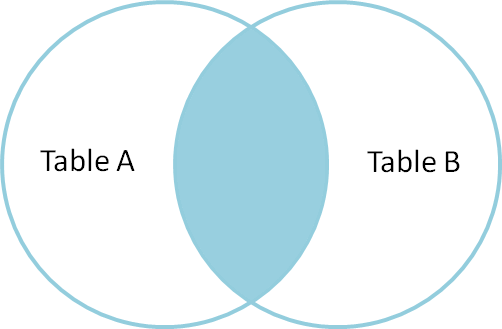
\includegraphics{notebooks/RW. Merging and Joining_files/figure-pdf/cell-33-output-1.png}

}

\end{figure}

(Image from
http://blog.codinghorror.com/a-visual-explanation-of-sql-joins/)

The inner join \emph{only} includes data whose index appears in both
tables. Let's see what that looks like:

\begin{Shaded}
\begin{Highlighting}[]
\NormalTok{df\_joined }\OperatorTok{=}\NormalTok{ df1.merge(df5, left\_index}\OperatorTok{=}\VariableTok{True}\NormalTok{, right\_index}\OperatorTok{=}\VariableTok{True}\NormalTok{)}
\end{Highlighting}
\end{Shaded}

\begin{Shaded}
\begin{Highlighting}[]
\NormalTok{df\_joined}
\end{Highlighting}
\end{Shaded}

\begin{longtable}[]{@{}lllllllll@{}}
\toprule\noalign{}
& area & population & mean temperature & elevation & annual rainfall &
Mean House Price & median income & walkability score \\
\midrule\noalign{}
\endhead
\bottomrule\noalign{}
\endlastfoot
London & 4.898594 & 6.625739 & 3.587877 & 6.063331 & 4.342769 & 4.848734
& 6.598818 & 5.442444 \\
Paris & 6.032702 & 3.479265 & 2.383832 & 5.251509 & 5.158178 & 5.294294
& 4.282418 & 5.741057 \\
\end{longtable}

Here, we have a couple of arguments specifying the manner of the join -
we have specified that we are joining on the index of the left and right
dataset with the optional ``left\_index=True'' and
``right\_index=True''. Less obviously, the \textbf{left} dataset is df1
(because we're using \emph{df1.merge()} and the \textbf{right} dataset
is df5 (because it appears as an argument in merge(). There's no special
reason it shouldn't be the other way around, but for this function, it
is this way around and we need to remember that when we use it.

\hypertarget{inner-space}{%
\section{Inner Space}\label{inner-space}}

Although we haven't specified it, the merge() function has defaulted to
an inner join (like the diagram above). We can specify how the join is
calculated by changing the text in the optional argument ``how'':

\begin{Shaded}
\begin{Highlighting}[]
\NormalTok{df\_joined }\OperatorTok{=}\NormalTok{ df1.merge(df5, left\_index}\OperatorTok{=}\VariableTok{True}\NormalTok{, right\_index}\OperatorTok{=}\VariableTok{True}\NormalTok{, how}\OperatorTok{=}\StringTok{\textquotesingle{}inner\textquotesingle{}}\NormalTok{)}
\end{Highlighting}
\end{Shaded}

\begin{Shaded}
\begin{Highlighting}[]
\NormalTok{df\_joined}
\end{Highlighting}
\end{Shaded}

\begin{longtable}[]{@{}lllllllll@{}}
\toprule\noalign{}
& area & population & mean temperature & elevation & annual rainfall &
Mean House Price & median income & walkability score \\
\midrule\noalign{}
\endhead
\bottomrule\noalign{}
\endlastfoot
London & 4.898594 & 6.625739 & 3.587877 & 6.063331 & 4.342769 & 4.848734
& 6.598818 & 5.442444 \\
Paris & 6.032702 & 3.479265 & 2.383832 & 5.251509 & 5.158178 & 5.294294
& 4.282418 & 5.741057 \\
\end{longtable}

\hypertarget{the-future-of-the-left}{%
\section{The Future of The Left}\label{the-future-of-the-left}}

The \emph{left} join includes \textbf{all} rows where the index appears
on the \textbf{left} hand side of the join, and \textbf{any} data which
\textbf{matches} it on the \textbf{right} hand side. If the index
appears on the left but not the right, it will include the data from the
left table, and have blanks for the columns on the right.

\begin{Shaded}
\begin{Highlighting}[]
\NormalTok{data\_path }\OperatorTok{=} \StringTok{"https://s3.eu{-}west{-}2.amazonaws.com/qm2/wk3/left.png"}
\NormalTok{Image(data\_path)}
\end{Highlighting}
\end{Shaded}

\begin{figure}[H]

{\centering 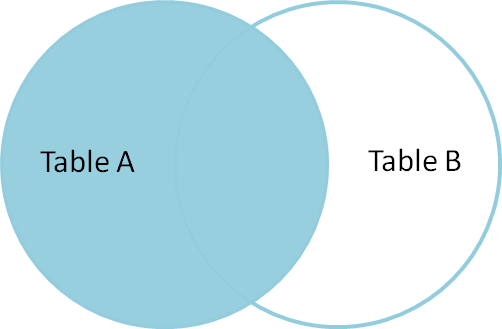
\includegraphics{notebooks/RW. Merging and Joining_files/figure-pdf/cell-38-output-1.png}

}

\end{figure}

What does \emph{this} look like? We will use the \emph{how=`left'}
optional argument to create a left join:

\begin{Shaded}
\begin{Highlighting}[]
\NormalTok{df\_joined }\OperatorTok{=}\NormalTok{ df1.merge(df5, left\_index}\OperatorTok{=}\VariableTok{True}\NormalTok{, right\_index}\OperatorTok{=}\VariableTok{True}\NormalTok{, how}\OperatorTok{=}\StringTok{\textquotesingle{}left\textquotesingle{}}\NormalTok{)}
\end{Highlighting}
\end{Shaded}

\begin{Shaded}
\begin{Highlighting}[]
\NormalTok{df\_joined}
\end{Highlighting}
\end{Shaded}

\begin{longtable}[]{@{}lllllllll@{}}
\toprule\noalign{}
& area & population & mean temperature & elevation & annual rainfall &
Mean House Price & median income & walkability score \\
\midrule\noalign{}
\endhead
\bottomrule\noalign{}
\endlastfoot
London & 4.898594 & 6.625739 & 3.587877 & 6.063331 & 4.342769 & 4.848734
& 6.598818 & 5.442444 \\
Paris & 6.032702 & 3.479265 & 2.383832 & 5.251509 & 5.158178 & 5.294294
& 4.282418 & 5.741057 \\
Beijing & 4.368419 & 4.993774 & 2.942992 & 3.761624 & 6.002863 & NaN &
NaN & NaN \\
Medellin & 7.437921 & 5.228150 & 3.902431 & 4.437361 & 5.563400 & NaN &
NaN & NaN \\
Port Elizabeth & 7.053265 & 5.936734 & 5.842155 & 6.042136 & 7.057592 &
NaN & NaN & NaN \\
\end{longtable}

As we see, the missing data appears as \textbf{NaN} - Not a Number.

\hypertarget{exercise-18}{%
\section{Exercise:}\label{exercise-18}}

Carry out \emph{right} and \emph{outer} joins on the dataframes df1 and
df5 and explain how they're filtering and joining the data.

\hypertarget{i-am-the-one-and-only}{%
\section{I Am The One and Only}\label{i-am-the-one-and-only}}

So far, we've carried out joins on data which have a \emph{one-to-one}
relationship; data for cities or people. What if our data has a
\emph{one-to-many} correspondence?

\emph{Example:} We want to look at the quality of life in cities (a real
student project from 2014). We have a dataset listing city-level
characteristics for a number of cities in Europe, including the country
each city is in. We also have a dataset listing the GDP, life expectancy
and other indicators for a number of \emph{countries} in Europe. How do
we create a dataframe which, for each city, lists all of the
characteristics of a city and those of its parent country?

We'll be working now with data from the UN, covering information about
cities - real data this time. The UN has some great data, we've taken
some from here and processed it in various ways:

http://data.un.org/Data.aspx?d=POP\&f=tableCode\%3A240

Let's load up data on city population - this set contains data for
2012-2014 inclusive:

\begin{Shaded}
\begin{Highlighting}[]
\NormalTok{data\_path }\OperatorTok{=} \StringTok{"data/wk5/UN\_Cities\_1214\_population.csv"}

\NormalTok{city\_pop }\OperatorTok{=}\NormalTok{ pd.read\_csv(data\_path, encoding}\OperatorTok{=}\StringTok{\textquotesingle{}latin1\textquotesingle{}}\NormalTok{)}
\end{Highlighting}
\end{Shaded}

\begin{Shaded}
\begin{Highlighting}[]
\NormalTok{city\_pop.head()}
\end{Highlighting}
\end{Shaded}

\begin{longtable}[]{@{}lllllllllll@{}}
\toprule\noalign{}
& Year & Area & Sex & City & City type & Record Type & Reliability &
Source Year & Value & Value Footnotes \\
\midrule\noalign{}
\endhead
\bottomrule\noalign{}
\endlastfoot
0 & 2013 & Total & Both Sexes & MARIEHAMN & City proper & Estimate - de
jure & Final figure, complete & 2014 & 11370.0 & NaN \\
1 & 2013 & Total & Male & MARIEHAMN & City proper & Estimate - de jure &
Final figure, complete & 2014 & 5445.0 & NaN \\
2 & 2013 & Total & Female & MARIEHAMN & City proper & Estimate - de jure
& Final figure, complete & 2014 & 5925.0 & NaN \\
3 & 2012 & Total & Both Sexes & MARIEHAMN & City proper & Estimate - de
jure & Final figure, complete & 2013 & 11304.5 & NaN \\
4 & 2012 & Total & Male & MARIEHAMN & City proper & Estimate - de jure &
Final figure, complete & 2013 & 5408.0 & NaN \\
\end{longtable}

\hypertarget{exercise-19}{%
\section{Exercise}\label{exercise-19}}

There is a another datafile we downloaded called
\emph{UN\_Cities\_1214\_country.csv}. This is saved to
\texttt{data/wk5/UN\_Cities\_1214\_country.csv} - Load this into a
dataframe called \emph{city\_c} with the city name as the index and view
it; then, using \emph{merge} on city name with city\_pop to create a new
dataframe called \emph{cities}. You'll probably get some errors. google
the error messages, or ask ChatGPT/Gemini to help you understand them.

\textbf{Hints:} You'll notice that the index \textbf{won't} be the
column you want to merge on in the city\_pop data. What column
\emph{should} you merge on in city\_pop? Which column should you merge
on in city\_c?

The syntax for merging on a \textbf{column} (which is not the index) is
to pass the column name to the optional `left\_on=' or `right\_on='
arguments. And we don't use right\_index=True (or left\_index=True),
depending on which we're using.

So for example: \textbf{df1.merge(df2, left\_on=`Name',
right\_index=True)} would join df1 (on the left) to df2 (on the right),
using the column `Name' on the left (df1) and the index column (whatever
that is) on the right (df2).

\hypertarget{a-footnote-about-footnotes}{%
\section{A footnote about footnotes}\label{a-footnote-about-footnotes}}

Just a quick note - if you look at the primary UN data, you'll see
footnotes which will confuse the hell out of Pandas. I've taken the
footnotes out, but you can use .tail() to see whether there's any junk
in the trunk, and remove it via a text editor.

\hypertarget{clean-data}{%
\section{Clean data}\label{clean-data}}

We need to simplify this data a bit in the following ways:

\begin{enumerate}
\def\labelenumi{\arabic{enumi}.}
\tightlist
\item
  I'm going to focus on one year (2012)
\item
  I'm going to just look at ``Both Sexes'' (not focus on one gender)
\item
  I'm going to get rid of a column of data (the `Value Footnotes'
  column) using the \emph{drop()} method.
\end{enumerate}

\begin{Shaded}
\begin{Highlighting}[]
\NormalTok{cities }\OperatorTok{=}\NormalTok{ cities[cities[}\StringTok{\textquotesingle{}Sex\textquotesingle{}}\NormalTok{]}\OperatorTok{==}\StringTok{\textquotesingle{}Both Sexes\textquotesingle{}}\NormalTok{]}
\NormalTok{cities }\OperatorTok{=}\NormalTok{ cities[cities[}\StringTok{\textquotesingle{}Year\textquotesingle{}}\NormalTok{]}\OperatorTok{==}\DecValTok{2012}\NormalTok{]}
\NormalTok{cities.drop(}\StringTok{\textquotesingle{}Value Footnotes\textquotesingle{}}\NormalTok{, axis}\OperatorTok{=}\DecValTok{1}\NormalTok{, inplace}\OperatorTok{=}\VariableTok{True}\NormalTok{)}
\end{Highlighting}
\end{Shaded}

\begin{verbatim}
NameError: ignored
\end{verbatim}

\begin{Shaded}
\begin{Highlighting}[]
\NormalTok{cities.head()}
\end{Highlighting}
\end{Shaded}

\hypertarget{extension-in-my-place}{%
\section{Extension: In My Place}\label{extension-in-my-place}}

The command I used to get rid of that column is \emph{cities.drop(`Value
Footnotes', axis=1, inplace=True)}. The syntax is not so complex - the
first argument, \emph{`Value Footnotes'}, is just the name of the
column; the second argument, \emph{axis=1}, tells Pandas to look for a
column to remove (instead of a row which has \emph{axis=0}); the third
and final argument, \emph{inplace=True}, is a command that tells Pandas
to edit \emph{inplace}, i.e.~to edit the dataframe (\emph{cities})
directly. When \emph{inplace} is False (the default), this command does
not directly edit cities, but instead provide an output. So the syntax
for that would be

new\_cities = cities.drop(`Value Footnotes', axis=1)

and new\_cities would be a version of \emph{cities} without the
offending column. This is usually the safer option.

\hypertarget{life-oh-life}{%
\section{Life, Oh Life}\label{life-oh-life}}

The UN also has useful data by country, so let's try and work with some
of that and join it up with our city data. Let's work with Life
Expectancy Data:

http://data.un.org/Data.aspx?d=WDI\&f=Indicator\_Code\%3ASP.DYN.LE00.IN

\begin{Shaded}
\begin{Highlighting}[]
\NormalTok{life }\OperatorTok{=}\NormalTok{ pd.read\_csv(}\StringTok{\textquotesingle{}https://s3.eu{-}west{-}2.amazonaws.com/qm2/wk3/UN\_Life\_all.csv\textquotesingle{}}\NormalTok{, index\_col}\OperatorTok{=}\DecValTok{0}\NormalTok{)}
\end{Highlighting}
\end{Shaded}

\begin{Shaded}
\begin{Highlighting}[]
\NormalTok{life.head()}
\end{Highlighting}
\end{Shaded}

\hypertarget{exercise-20}{%
\section{Exercise:}\label{exercise-20}}

In a new cell, clean up the above dataframe by

\begin{itemize}
\tightlist
\item
  removing the ``Value Footnotes'' Column
\item
  use only the most recent data (2012)
\end{itemize}

Let's make it a little clearer what ``Value'' refers to, by renaming the
column. This is one way to do that:

\begin{Shaded}
\begin{Highlighting}[]
\NormalTok{life.rename(columns}\OperatorTok{=}\NormalTok{\{}\StringTok{\textquotesingle{}Value\textquotesingle{}}\NormalTok{:}\StringTok{\textquotesingle{}Life Expectancy\textquotesingle{}}\NormalTok{\}, inplace}\OperatorTok{=}\VariableTok{True}\NormalTok{)}
\end{Highlighting}
\end{Shaded}

\begin{Shaded}
\begin{Highlighting}[]
\NormalTok{life.head()}
\end{Highlighting}
\end{Shaded}

Now, merge this data with the cities data to show life expectancy for
each city (based on the country it is in), and show the first 5 rows.

Plot population against life expectancy. Use plot's \emph{optional
arguments} to specify the x column, y column, and that kind=`scatter'.

Question: How much data was ``missing'' in the merge?

\bookmarksetup{startatroot}

\hypertarget{hypothesis-testing}{%
\chapter{Hypothesis Testing}\label{hypothesis-testing}}

\hypertarget{workshop-7-open-in-colab}{%
\section[\emph{Workshop 7} ]{\texorpdfstring{\emph{Workshop 7}
\href{https://colab.research.google.com/github/oballinger/QM2/blob/main/notebooks/W07.\%20Hypothesis\%20Testing.ipynb}{\protect
\includegraphics{index_files/mediabag/colab-badge.png}}}{Workshop 7 Open In Colab}}\label{workshop-7-open-in-colab}}

For the rest of this course, we'll be working with data from the U.S.
Census \href{https://www.census.gov/programs-surveys/cps.html}{Current
Population Survey (CPS)}.

\hypertarget{aims-4}{%
\subsection{Aims:}\label{aims-4}}

\begin{itemize}
\tightlist
\item
  Understanding:

  \begin{itemize}
  \tightlist
  \item
    Confidence Intervals
  \item
    Hypothesis Testing

    \begin{enumerate}
    \def\labelenumi{\arabic{enumi}.}
    \tightlist
    \item
      Stating the Null and Alternative Hypotheses
    \item
      Selecting a Critical Value
    \item
      Calculating the Test Statistic
    \item
      Making a Decision
    \end{enumerate}
  \end{itemize}
\end{itemize}

\hypertarget{getting-started-2}{%
\section{Getting Started}\label{getting-started-2}}

We will be following on from the analysis we conducted in Workshop 5
(Distributions and Basic Statistics). We visually explored differences
in the income levels between different groups of people in the US
census. Now, we are going to conduct hypothesis testing to see if those
differences are statistically significant.

\begin{Shaded}
\begin{Highlighting}[]
\OperatorTok{!}\NormalTok{mkdir data}
\OperatorTok{!}\NormalTok{mkdir data}\OperatorTok{/}\NormalTok{wk7}
\OperatorTok{!}\NormalTok{curl https:}\OperatorTok{//}\NormalTok{storage.googleapis.com}\OperatorTok{/}\NormalTok{qm2}\OperatorTok{/}\NormalTok{wk7}\OperatorTok{/}\NormalTok{cps.csv }\OperatorTok{{-}}\NormalTok{o data}\OperatorTok{/}\NormalTok{wk7}\OperatorTok{/}\NormalTok{cps.csv}
\end{Highlighting}
\end{Shaded}

\begin{verbatim}
mkdir: data: File exists
mkdir: data/wk7: File exists
  % Total    % Received % Xferd  Average Speed   Time    Time     Time  Current
                                 Dload  Upload   Total   Spent    Left  Speed
100 22.4M  100 22.4M    0     0  16.5M      0  0:00:01  0:00:01 --:--:-- 16.6M
\end{verbatim}

\begin{Shaded}
\begin{Highlighting}[]
\CommentTok{\#This tells python to draw the graphs "inline" {-} in the notebook}
\OperatorTok{\%}\NormalTok{matplotlib inline  }
\ImportTok{import}\NormalTok{ matplotlib.pyplot }\ImportTok{as}\NormalTok{ plt}
\ImportTok{from}\NormalTok{ scipy.stats }\ImportTok{import}\NormalTok{ norm}
\ImportTok{import}\NormalTok{ statistics}
\ImportTok{import}\NormalTok{ seaborn }\ImportTok{as}\NormalTok{ sns}

\ImportTok{import}\NormalTok{ pylab}
\ImportTok{import}\NormalTok{ pandas }\ImportTok{as}\NormalTok{ pd}
\ImportTok{import}\NormalTok{ numpy }\ImportTok{as}\NormalTok{ np}
\CommentTok{\# make the plots (graphs) a little wider by default}
\NormalTok{pylab.rcParams[}\StringTok{\textquotesingle{}figure.figsize\textquotesingle{}}\NormalTok{] }\OperatorTok{=}\NormalTok{ (}\FloatTok{10.}\NormalTok{, }\FloatTok{8.}\NormalTok{)}
\NormalTok{sns.}\BuiltInTok{set}\NormalTok{(font\_scale}\OperatorTok{=}\FloatTok{1.5}\NormalTok{)}
\NormalTok{sns.set\_style(}\StringTok{"white"}\NormalTok{)}
\end{Highlighting}
\end{Shaded}

\begin{Shaded}
\begin{Highlighting}[]
\NormalTok{df}\OperatorTok{=}\NormalTok{pd.read\_csv(}\StringTok{\textquotesingle{}./data/wk7/cps.csv\textquotesingle{}}\NormalTok{)}
\NormalTok{df[}\StringTok{\textquotesingle{}race\textquotesingle{}}\NormalTok{]}\OperatorTok{=}\NormalTok{df[}\StringTok{\textquotesingle{}race\textquotesingle{}}\NormalTok{].astype(}\StringTok{\textquotesingle{}category\textquotesingle{}}\NormalTok{)}
\NormalTok{df[}\StringTok{\textquotesingle{}income\textquotesingle{}}\NormalTok{]}\OperatorTok{=}\NormalTok{df[}\StringTok{\textquotesingle{}incwage\textquotesingle{}}\NormalTok{]}\OperatorTok{/}\DecValTok{1000}
\NormalTok{df}\OperatorTok{=}\NormalTok{df[df[}\StringTok{\textquotesingle{}income\textquotesingle{}}\NormalTok{]}\OperatorTok{\textless{}}\DecValTok{200}\NormalTok{]}
\NormalTok{df}\OperatorTok{=}\NormalTok{df[df[}\StringTok{\textquotesingle{}year\textquotesingle{}}\NormalTok{]}\OperatorTok{==}\DecValTok{2013}\NormalTok{] }\CommentTok{\# filter the dataframe to only contain 2013 data}
\NormalTok{df.head()}
\end{Highlighting}
\end{Shaded}

\begin{longtable}[]{@{}lllllllllllll@{}}
\toprule\noalign{}
& year & state & age & sex & race & sch & ind & union & incwage &
realhrwage & occupation & income \\
\midrule\noalign{}
\endhead
\bottomrule\noalign{}
\endlastfoot
20 & 2013 & 50 & 62 & 1 & 1 & 14.0 & 8090 & 1.0 & 57000.0 & 23.889143 &
. & 57.0 \\
32 & 2013 & 39 & 59 & 1 & 1 & 13.0 & 9590 & 0.0 & 62000.0 & 29.726475 &
Consruction, Extraction, Installation & 62.0 \\
34 & 2013 & 44 & 44 & 1 & 3 & 12.0 & 7290 & 0.0 & 45000.0 & 20.745834 &
. & 45.0 \\
36 & 2013 & 12 & 41 & 1 & 1 & 12.0 & 7070 & 1.0 & 28000.0 & 12.293828 &
Managers & 28.0 \\
37 & 2013 & 33 & 35 & 1 & 1 & 12.0 & 770 & 0.0 & 42500.0 & 20.377020 &
Transportation and materials moving & 42.5 \\
\end{longtable}

This is once again the U.S. census data from Week 5. As a reminder, our
dataframe has 10 columns:

\begin{enumerate}
\def\labelenumi{\arabic{enumi}.}
\tightlist
\item
  \emph{year}: Survey year
\item
  \emph{age}: the person's age
\item
  \emph{sex}: the person's sex

  \begin{itemize}
  \tightlist
  \item
    1=male
  \item
    2=female
  \end{itemize}
\item
  \emph{race}: the person's race

  \begin{itemize}
  \tightlist
  \item
    White non hispanic=1
  \item
    Black non hispanic=2
  \item
    Hispanic=3
  \item
    Other non hispanic=4)
  \end{itemize}
\item
  \emph{sch}: Educational attainment

  \begin{itemize}
  \tightlist
  \item
    None = 0,
  \item
    Grades 1-12 = 1-12
  \item
    Some University = 13,
  \item
    Associate's degree = 14,
  \item
    BA = 16
  \item
    Advanced Degree = 18
  \end{itemize}
\item
  \emph{union}: Union membership

  \begin{itemize}
  \tightlist
  \item
    N/A = 0,
  \item
    No union coverage = 1,
  \item
    Member of labor union=2,
  \item
    Covered by union but not a member=3
  \end{itemize}
\item
  \emph{incwage}: Wage and salary income
\item
  \emph{realhrwage}: Real Hourly Wage
\item
  \emph{occupation}: Occupation
\item
  \emph{ind}:
  \href{https://www.census.gov/naics/?58967?yearbck=2002}{industry code}
\end{enumerate}

\hypertarget{confidence-intervals}{%
\section{Confidence Intervals}\label{confidence-intervals}}

So far in this workshop, we've had the luxury of being able to draw many
random samples and plot the distributions of their sample means to infer
the population mean. The Central Limit Theorem lets us assume that these
sample means are normally distributed, and consequently that there is a
95.45\% chance that the \textbf{population mean} within two standard
errors of the \textbf{sample mean}. This allows us to make inferences on
the basis of \emph{a single sample}. The standard error is the

\hypertarget{sample-standard-deviation}{%
\subsection{Sample Standard Deviation}\label{sample-standard-deviation}}

\[\huge s = \sqrt{\frac{1}{n-1} \sum_{i=1}^n (x_i - \overline{x})^2}\]

\hypertarget{standard-error}{%
\subsection{Standard Error}\label{standard-error}}

\[\huge se = \frac{s}{\sqrt{n}}\]

Given a large enough sample \(x\), we can build a 95\% confidence
interval as follows:

\[ \huge 95\% CI = \overline{x} \pm (1.96 \times se)\]

Let's draw a sample of 1000 random individuals from our data, and
compute a 95\% confidence interval to estimate the population mean for
income. We'll begin by creating a swarmplot to get a sense of how the
data are distributed.

\begin{Shaded}
\begin{Highlighting}[]
\NormalTok{sample}\OperatorTok{=}\NormalTok{df.sample(}\DecValTok{1000}\NormalTok{) }\CommentTok{\# draw a random sample of 1000 observations from the dataframe}
\NormalTok{sns.swarmplot(data }\OperatorTok{=}\NormalTok{ sample, y}\OperatorTok{=}\StringTok{\textquotesingle{}income\textquotesingle{}}\NormalTok{) }\CommentTok{\# plot a swarmplot of income}
\NormalTok{plt.title(}\StringTok{\textquotesingle{}Income Distribution\textquotesingle{}}\NormalTok{) }\CommentTok{\# add a title}
\end{Highlighting}
\end{Shaded}

\begin{verbatim}
Text(0.5, 1.0, 'Income Distribution')
\end{verbatim}

\begin{figure}[H]

{\centering \includegraphics{notebooks/W06. Hypothesis Testing_files/figure-pdf/cell-5-output-2.png}

}

\end{figure}

Now let's set about calculating the 95\% confidence interval and
plotting it on our swarmplot. Luckily, the components we need to this
are easy to calculate. We just need the mean, standard deviation, and
number of observations. All of these are provided by the
\texttt{.describe()} function, which calculates summary statistics for a
sample.

\begin{Shaded}
\begin{Highlighting}[]
\NormalTok{desc}\OperatorTok{=}\NormalTok{sample[}\StringTok{\textquotesingle{}income\textquotesingle{}}\NormalTok{].describe() }\CommentTok{\# calculate descriptive statistics for the sample}
\BuiltInTok{print}\NormalTok{(desc) }\CommentTok{\# print the descriptive statistics}
\end{Highlighting}
\end{Shaded}

\begin{verbatim}
count    1000.000000
mean       47.677568
std        33.041244
min         0.700000
25%        25.000000
50%        40.000000
75%        62.000000
max       190.000000
Name: income, dtype: float64
\end{verbatim}

From the set of descriptive statistics, we can pull out the relevant
components, calculate the standard error, and create a 95\% confidence
interval as follows:

\begin{Shaded}
\begin{Highlighting}[]
\NormalTok{mean}\OperatorTok{=}\NormalTok{desc[}\StringTok{\textquotesingle{}mean\textquotesingle{}}\NormalTok{] }\CommentTok{\# set the mean equal to a variable called "mean"}
\NormalTok{std}\OperatorTok{=}\NormalTok{desc[}\StringTok{\textquotesingle{}std\textquotesingle{}}\NormalTok{] }\CommentTok{\# set the standard deviation equal to a variable called "std"}
\NormalTok{n}\OperatorTok{=}\NormalTok{desc[}\StringTok{\textquotesingle{}count\textquotesingle{}}\NormalTok{] }\CommentTok{\# set the sample size equal to a variable called "n"}
\NormalTok{se}\OperatorTok{=}\NormalTok{std}\OperatorTok{/}\NormalTok{np.sqrt(n) }\CommentTok{\# calculate the standard error of the mean}

\BuiltInTok{print}\NormalTok{(}\StringTok{\textquotesingle{}The mean is\textquotesingle{}}\NormalTok{, }\BuiltInTok{round}\NormalTok{(mean, }\DecValTok{2}\NormalTok{), }\StringTok{\textquotesingle{}with a standard error of\textquotesingle{}}\NormalTok{, }\BuiltInTok{round}\NormalTok{(se, }\DecValTok{2}\NormalTok{)) }\CommentTok{\# print the mean and standard error}

\NormalTok{upper\_ci }\OperatorTok{=}\NormalTok{ mean}\OperatorTok{+}\NormalTok{se}\OperatorTok{*}\FloatTok{1.96} \CommentTok{\# calculate the upper confidence interval}
\NormalTok{lower\_ci }\OperatorTok{=}\NormalTok{ mean}\OperatorTok{{-}}\NormalTok{se}\OperatorTok{*}\FloatTok{1.96} \CommentTok{\# calculate the lower confidence interval}

\BuiltInTok{print}\NormalTok{(}\StringTok{\textquotesingle{}The 95}\SpecialCharTok{\% c}\StringTok{onfidence interval is\textquotesingle{}}\NormalTok{, }\BuiltInTok{round}\NormalTok{(lower\_ci, }\DecValTok{2}\NormalTok{), }\StringTok{\textquotesingle{}to\textquotesingle{}}\NormalTok{, }\BuiltInTok{round}\NormalTok{(upper\_ci, }\DecValTok{2}\NormalTok{)) }\CommentTok{\# print the confidence interval}
\end{Highlighting}
\end{Shaded}

\begin{verbatim}
The mean is 47.68 with a standard error of 1.04
The 95% confidence interval is 45.63 to 49.73
\end{verbatim}

Finally, let's plot these bounds on our swarmplot to graphically show
this range. We can now claim that based on our sample, there is a 95\%
chance that the true population mean of income (shown in red) lies
within this range.

\begin{Shaded}
\begin{Highlighting}[]
\NormalTok{sns.swarmplot(data }\OperatorTok{=}\NormalTok{ sample, y}\OperatorTok{=}\StringTok{\textquotesingle{}income\textquotesingle{}}\NormalTok{,alpha}\OperatorTok{=}\FloatTok{0.5}\NormalTok{) }\CommentTok{\# plot a swarmplot of income}
\NormalTok{plt.axhline(df[}\StringTok{\textquotesingle{}income\textquotesingle{}}\NormalTok{].mean(), color}\OperatorTok{=}\StringTok{\textquotesingle{}red\textquotesingle{}}\NormalTok{, linestyle}\OperatorTok{=}\StringTok{\textquotesingle{}solid\textquotesingle{}}\NormalTok{, linewidth}\OperatorTok{=}\DecValTok{3}\NormalTok{, label}\OperatorTok{=}\StringTok{\textquotesingle{}Population Mean\textquotesingle{}}\NormalTok{) }\CommentTok{\# add a horizontal line at the mean}
\NormalTok{plt.axhline(upper\_ci, color}\OperatorTok{=}\StringTok{\textquotesingle{}black\textquotesingle{}}\NormalTok{, linestyle}\OperatorTok{=}\StringTok{\textquotesingle{}dashed\textquotesingle{}}\NormalTok{, linewidth}\OperatorTok{=}\DecValTok{3}\NormalTok{) }\CommentTok{\# add a dashed black line at the upper confidence interval}
\NormalTok{plt.axhline(lower\_ci, color}\OperatorTok{=}\StringTok{\textquotesingle{}black\textquotesingle{}}\NormalTok{, linestyle}\OperatorTok{=}\StringTok{\textquotesingle{}dashed\textquotesingle{}}\NormalTok{, linewidth}\OperatorTok{=}\DecValTok{3}\NormalTok{) }\CommentTok{\# add a dashed black line at the lower confidence interval}

\NormalTok{plt.title(}\StringTok{\textquotesingle{}Income Distribution, 95\% Confidence Interval\textquotesingle{}}\NormalTok{) }\CommentTok{\# add a title}
\end{Highlighting}
\end{Shaded}

\begin{verbatim}
Text(0.5, 1.0, 'Income Distribution, 95% Confidence Interval')
\end{verbatim}

\begin{figure}[H]

{\centering 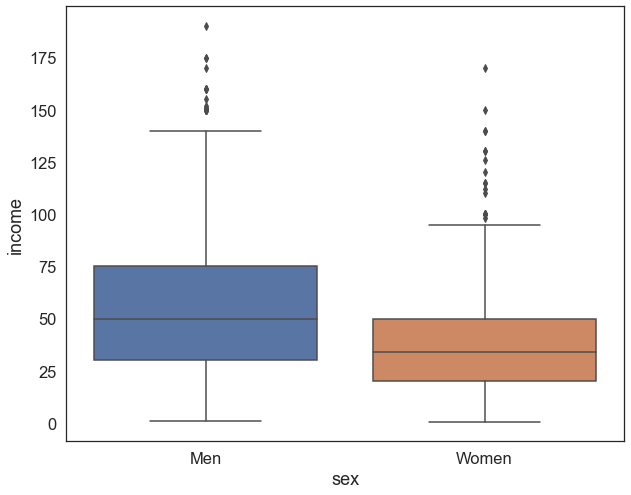
\includegraphics{notebooks/W06. Hypothesis Testing_files/figure-pdf/cell-8-output-2.png}

}

\end{figure}

\hypertarget{hypothesis-testing-1}{%
\section{Hypothesis Testing}\label{hypothesis-testing-1}}

If we create a boxplot of income disaggregated by sex using our sample,
we can observe that men seem to earn more than women:

\begin{Shaded}
\begin{Highlighting}[]
\NormalTok{sns.boxplot(data}\OperatorTok{=}\NormalTok{sample , x}\OperatorTok{=}\StringTok{\textquotesingle{}sex\textquotesingle{}}\NormalTok{, y}\OperatorTok{=}\StringTok{\textquotesingle{}income\textquotesingle{}}\NormalTok{).set\_xticklabels([}\StringTok{\textquotesingle{}Men\textquotesingle{}}\NormalTok{,}\StringTok{\textquotesingle{}Women\textquotesingle{}}\NormalTok{]) }\CommentTok{\# make a box plot of income by sex}
\end{Highlighting}
\end{Shaded}

\begin{verbatim}
[Text(0, 0, 'Men'), Text(1, 0, 'Women')]
\end{verbatim}

\begin{figure}[H]

{\centering \includegraphics{notebooks/W06. Hypothesis Testing_files/figure-pdf/cell-9-output-2.png}

}

\end{figure}

But is this difference statistically significant? It could just be due
to sampling error, random chance. \textbf{Hypothesis testing} provides a
framework through which we can formally evaluate the likelihood of
encountering an effect as extreme (in this case, the the difference
between the mean incomes between both groups) as the one we observe in
our data. There are four main steps in hypothesis testing:

\begin{enumerate}
\def\labelenumi{\arabic{enumi}.}
\tightlist
\item
  State the hypotheses. H0 states that there is no difference between
  the two population means.
\item
  Select an \(\alpha\) level (e.g.~95\% confidence), and select a
  corresponding \textbf{critical value} (1.96 for large samples)
\item
  Compute the test statistic.
\item
  Make a decision; if the test statistic exceeds the critical value, we
  \textbf{reject the null hypothesis}.
\end{enumerate}

Steps 1, 2, and 4 remain fairly constant regardless of what kind of
hypothesis testing you're conducting. Step 3 can vary quite a bit, as
there are many different statistical tests that fall under the umbrella
of hypothesis testing. In today's workshop we'll be using the Student's
T-Test (more on that in a second). For now, let's begin the process of
hypothesis testing a

\hypertarget{state-the-hypotheses}{%
\subsection{1. State the hypotheses}\label{state-the-hypotheses}}

\hypertarget{the-null-hypothesis}{%
\subsubsection{The Null Hypothesis}\label{the-null-hypothesis}}

\begin{itemize}
\tightlist
\item
  \(H_0\) : There is no difference in the mean income between men and
  women
\item
  \(H_0\) : \(\overline{x}_{men} = \overline{x}_{women}\)
\end{itemize}

\hypertarget{the-alternative-hypothesis}{%
\subsubsection{The Alternative
Hypothesis}\label{the-alternative-hypothesis}}

\begin{itemize}
\tightlist
\item
  \(H_a\) : There is a difference in the mean income between men and
  women
\item
  \(H_a\) : \(\overline{x}_{men} \neq \overline{x}_{women}\)
\end{itemize}

\hypertarget{select-an-alpha-level}{%
\subsection{\texorpdfstring{2. Select an \(\alpha\)
level}{2. Select an \textbackslash alpha level}}\label{select-an-alpha-level}}

Locate the critical region; the critical values for the t statistic are
obtained using degrees of freedom (\(df=n-2\)). Given that we have 1000
observations, \(df=998\). If \(df>1000\), you can simply memorize the
following critical values:

\begin{itemize}
\tightlist
\item
  At the 95\% confidence level, the critical value is 1.96
\item
  At the 99\% confidence level, the critical value is 2.58
\end{itemize}

If our test statistic exceeds either of these values, we can reject the
null hypothesis with the according level of confidence. The function
below creates a plot which provides a visual reference for these values,
but isn't really necessary for the process of hypothesis testing. The
function accepts one argument \texttt{test\_statistic}, which it will
use to plot a vertical red line. If the red line falls within the dotted
lines, we fail to reject the null hypothesis at the corresponding
confidence level. If it's outside of these bounds, we reject the null
hypothesis.

In the last line of code below, i've called the function to plot a test
statistic of -2.3; Would we reject the null hypothesis at the 95\%
confidence level? what about the 99\% level?

\begin{Shaded}
\begin{Highlighting}[]
\KeywordTok{def}\NormalTok{ plot\_z(test\_statistic):}
\NormalTok{    mu, se}\OperatorTok{=} \DecValTok{0}\NormalTok{, }\DecValTok{1} \CommentTok{\# create two variables, a mean "mu" equal to zero, and standard deviation "se" equal to 1}
\NormalTok{    x }\OperatorTok{=}\NormalTok{ np.linspace(mu }\OperatorTok{{-}} \DecValTok{3}\OperatorTok{*}\NormalTok{se, mu }\OperatorTok{+} \DecValTok{3}\OperatorTok{*}\NormalTok{se, }\DecValTok{100}\NormalTok{) }\CommentTok{\# create a range of values from {-}3 to 3 standard deviations}

\NormalTok{    plt.plot(x, norm.pdf(x, mu, se)) }\CommentTok{\# plot the normal distribution}
\NormalTok{    plt.axvline(mu}\OperatorTok{{-}}\NormalTok{se}\OperatorTok{*}\FloatTok{1.96}\NormalTok{, color}\OperatorTok{=}\StringTok{\textquotesingle{}blue\textquotesingle{}}\NormalTok{, linestyle}\OperatorTok{=}\StringTok{\textquotesingle{}dashed\textquotesingle{}}\NormalTok{, linewidth}\OperatorTok{=}\FloatTok{1.5}\NormalTok{,label}\OperatorTok{=}\StringTok{\textquotesingle{}µ ± 1.96σ (95}\SpecialCharTok{\% c}\StringTok{onfidence)\textquotesingle{}}\NormalTok{) }\CommentTok{\# plot a vertical line at the mean plus 2 standard deviations}
\NormalTok{    plt.axvline(mu}\OperatorTok{+}\NormalTok{se}\OperatorTok{*}\FloatTok{1.96}\NormalTok{, color}\OperatorTok{=}\StringTok{\textquotesingle{}blue\textquotesingle{}}\NormalTok{, linestyle}\OperatorTok{=}\StringTok{\textquotesingle{}dashed\textquotesingle{}}\NormalTok{, linewidth}\OperatorTok{=}\FloatTok{1.5}\NormalTok{)  }\CommentTok{\# plot a vertical line at the mean minus 2 standard deviations}
\NormalTok{    plt.axvline(mu}\OperatorTok{{-}}\NormalTok{se}\OperatorTok{*}\FloatTok{2.58}\NormalTok{, color}\OperatorTok{=}\StringTok{\textquotesingle{}green\textquotesingle{}}\NormalTok{, linestyle}\OperatorTok{=}\StringTok{\textquotesingle{}dashed\textquotesingle{}}\NormalTok{, linewidth}\OperatorTok{=}\FloatTok{1.5}\NormalTok{,label}\OperatorTok{=}\StringTok{\textquotesingle{}µ ± 2.58σ (99}\SpecialCharTok{\% c}\StringTok{onfidence)\textquotesingle{}}\NormalTok{) }\CommentTok{\# plot a vertical line at the mean plus 2 standard deviations}
\NormalTok{    plt.axvline(mu}\OperatorTok{+}\NormalTok{se}\OperatorTok{*}\FloatTok{2.58}\NormalTok{, color}\OperatorTok{=}\StringTok{\textquotesingle{}green\textquotesingle{}}\NormalTok{, linestyle}\OperatorTok{=}\StringTok{\textquotesingle{}dashed\textquotesingle{}}\NormalTok{, linewidth}\OperatorTok{=}\FloatTok{1.5}\NormalTok{)  }\CommentTok{\# plot a vertical line at the mean minus 2 standard deviations}
    
\NormalTok{    plt.axvline(test\_statistic, color}\OperatorTok{=}\StringTok{\textquotesingle{}red\textquotesingle{}}\NormalTok{, linestyle}\OperatorTok{=}\StringTok{\textquotesingle{}solid\textquotesingle{}}\NormalTok{, linewidth}\OperatorTok{=}\FloatTok{1.5}\NormalTok{,label}\OperatorTok{=}\StringTok{\textquotesingle{}Test Statistic\textquotesingle{}}\NormalTok{) }\CommentTok{\# plot a vertical line at the test statistic}


\NormalTok{    plt.ylim(}\DecValTok{0}\NormalTok{,}\FloatTok{0.4}\NormalTok{)}
\NormalTok{    plt.legend()}
\NormalTok{    plt.title(}\StringTok{\textquotesingle{}Z Distribution\textquotesingle{}}\NormalTok{) }\CommentTok{\# add a title}
\NormalTok{    plt.show()}

\NormalTok{plot\_z(}\OperatorTok{{-}}\FloatTok{2.3}\NormalTok{)}
\end{Highlighting}
\end{Shaded}

\begin{figure}[H]

{\centering 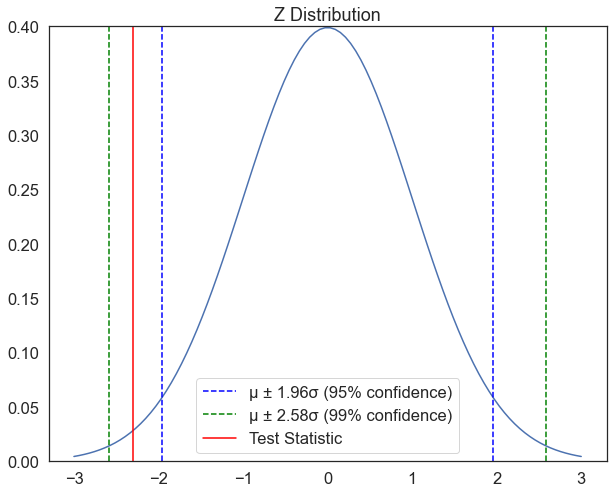
\includegraphics{notebooks/W06. Hypothesis Testing_files/figure-pdf/cell-10-output-1.png}

}

\end{figure}

\hypertarget{calculate-the-test-statistic-the-students-t-test}{%
\subsection{3. Calculate the Test Statistic (The Student's
T-Test)}\label{calculate-the-test-statistic-the-students-t-test}}

The Student's T-Test is an \emph{independent-measures design} which is
used in situations where a researcher has no prior knowledge about
either of the two populations (or treatments) being compared. In
particular, the population means and standard deviations are all
unknown. Because the population variances are not known, these values
must be estimated from the sample data.

The purpose of a T-test is to determine whether the sample mean
difference indicates a real mean difference between the two populations
or whether the obtained difference is simply the result of sampling
error. Given two groups, \(x_1\) and \(x_2\), the \(t\) statistic is
calculated as:

\[ \Huge t = {\frac{\overline{x_1}-\overline{x_2}} {\sqrt{\frac{s^2_1}{n_1} + \frac{s^2_2}{n_2}}}} \]

Where:

\begin{itemize}
\tightlist
\item
  \(\overline{x}\): Sample Mean
\item
  \(s^2\): Sample Standard Deviation
\item
  \(n\): Number of observations
\end{itemize}

We've already seen how to calculate each of these components when we
made the 95\% confidence interval above using the \texttt{.describe()}
function. To calculate the t-statistic, we just have to plug these
values into the formula above and do some basic arithmetic. I've put
together a function that does this below, which accepts two main
arguments, \texttt{group1} and \texttt{group2}. For each group it
calculates descriptive statistics, and uses these values to calculate
the t-statistic. It also has an optional argument \texttt{plot}, which
when set to \texttt{True} will plot a 95\% confidence interval for each
group. It defaults to \texttt{False}, meaning that it won't generate the
plot.

\begin{Shaded}
\begin{Highlighting}[]
\KeywordTok{def}\NormalTok{ manual\_ttest(group1, group2, plot}\OperatorTok{=}\VariableTok{False}\NormalTok{): }\CommentTok{\# define a function called "manual\_ttest" that takes two groups and a boolean value for whether or not to plot the results as arguments}
    
\NormalTok{    desc1, desc2}\OperatorTok{=}\NormalTok{group1.describe(), group2.describe() }\CommentTok{\# get descriptive statistics for both samples}
    
\NormalTok{    n1,std1,mean1 }\OperatorTok{=}\NormalTok{ desc1[}\StringTok{\textquotesingle{}count\textquotesingle{}}\NormalTok{], desc1[}\StringTok{\textquotesingle{}std\textquotesingle{}}\NormalTok{] ,desc1[}\StringTok{\textquotesingle{}mean\textquotesingle{}}\NormalTok{] }\CommentTok{\# get the sample size, standard deviation, and mean of the first sample}
\NormalTok{    n2,std2,mean2 }\OperatorTok{=}\NormalTok{ desc2[}\StringTok{\textquotesingle{}count\textquotesingle{}}\NormalTok{], desc2[}\StringTok{\textquotesingle{}std\textquotesingle{}}\NormalTok{] ,desc2[}\StringTok{\textquotesingle{}mean\textquotesingle{}}\NormalTok{] }\CommentTok{\# get the sample size, standard deviation, and mean of the second sample}
    
    \CommentTok{\# calculate standard errors}
\NormalTok{    se1, se2 }\OperatorTok{=}\NormalTok{ std1}\OperatorTok{**}\DecValTok{2}\OperatorTok{/}\NormalTok{n1, std2}\OperatorTok{**}\DecValTok{2}\OperatorTok{/}\NormalTok{n2 }\CommentTok{\# \textquotesingle{}**2\textquotesingle{} is the same as squaring the number}

    \CommentTok{\# standard error on the difference between the samples}
\NormalTok{    sed }\OperatorTok{=}\NormalTok{ np.sqrt(se1 }\OperatorTok{+}\NormalTok{ se2)}

    \CommentTok{\# calculate the t statistic}
\NormalTok{    t\_stat }\OperatorTok{=}\NormalTok{ (mean1 }\OperatorTok{{-}}\NormalTok{ mean2) }\OperatorTok{/}\NormalTok{ sed}

    \CommentTok{\# print the results}
    \BuiltInTok{print}\NormalTok{(}\StringTok{"Group 1: n=\%.0f, mean=}\SpecialCharTok{\%.3f}\StringTok{, std=}\SpecialCharTok{\%.3f}\StringTok{"} \OperatorTok{\%}\NormalTok{ (n1,mean1,std1)) }
    \BuiltInTok{print}\NormalTok{(}\StringTok{"Group 2: n=\%.0f, mean=}\SpecialCharTok{\%.3f}\StringTok{, std=}\SpecialCharTok{\%.3f}\StringTok{"} \OperatorTok{\%}\NormalTok{ (n2,mean2,std2))}
    \BuiltInTok{print}\NormalTok{(}\StringTok{\textquotesingle{}The t{-}statistic is }\SpecialCharTok{\%.3f}\StringTok{\textquotesingle{}} \OperatorTok{\%}\NormalTok{ t\_stat) }\CommentTok{\# print the t{-}statistic}

    \ControlFlowTok{if}\NormalTok{ plot}\OperatorTok{==}\VariableTok{True}\NormalTok{: }\CommentTok{\# if the plot argument is set to True, plot the results}
\NormalTok{        groups}\OperatorTok{=}\NormalTok{pd.DataFrame() }\CommentTok{\# create an empty dataframe}
\NormalTok{        i}\OperatorTok{=}\DecValTok{1} \CommentTok{\# create a counter variable called "i" and set it equal to 1}
        
        \ControlFlowTok{for}\NormalTok{ group }\KeywordTok{in}\NormalTok{ [group1, group2]: }\CommentTok{\# loop through each group in the list of groups}
\NormalTok{            plot\_df}\OperatorTok{=}\NormalTok{pd.DataFrame(\{}\StringTok{\textquotesingle{}Values\textquotesingle{}}\NormalTok{: group,}\StringTok{\textquotesingle{}Group\textquotesingle{}}\NormalTok{:i\}) }\CommentTok{\# create a dataframe with the values of the group and a column called "Group" that contains the group number}
\NormalTok{            groups}\OperatorTok{=}\NormalTok{groups.append(plot\_df) }\CommentTok{\# append the dataframe to the list of dataframes}
\NormalTok{            i}\OperatorTok{+=}\DecValTok{1} \CommentTok{\# increase the counter by 1}
        
\NormalTok{        sns.pointplot(data}\OperatorTok{=}\NormalTok{groups , x}\OperatorTok{=}\StringTok{\textquotesingle{}Group\textquotesingle{}}\NormalTok{, y}\OperatorTok{=}\StringTok{\textquotesingle{}Values\textquotesingle{}}\NormalTok{,errorbar}\OperatorTok{=}\NormalTok{(}\StringTok{\textquotesingle{}ci\textquotesingle{}}\NormalTok{, }\DecValTok{95}\NormalTok{), color}\OperatorTok{=}\StringTok{\textquotesingle{}black\textquotesingle{}}\NormalTok{, join}\OperatorTok{=}\VariableTok{False}\NormalTok{, capsize}\OperatorTok{=}\FloatTok{.8}\NormalTok{) }\CommentTok{\# plot the means of the groups with a 95\% confidence interval}
\NormalTok{        plt.title(}\StringTok{\textquotesingle{}Comparison of Group Means with 95\% Confidence Intervals\textquotesingle{}}\NormalTok{) }\CommentTok{\# add a title}
    
    \ControlFlowTok{return}\NormalTok{ t\_stat }\CommentTok{\# return the t{-}statistic}
\end{Highlighting}
\end{Shaded}

Having defined the function, we can now call it to calculate a t-test
for the difference in income between men and women

\begin{Shaded}
\begin{Highlighting}[]
\NormalTok{men}\OperatorTok{=}\NormalTok{sample[sample[}\StringTok{\textquotesingle{}sex\textquotesingle{}}\NormalTok{]}\OperatorTok{==}\DecValTok{1}\NormalTok{] }\CommentTok{\# filter the sample to only include men}
\NormalTok{women}\OperatorTok{=}\NormalTok{sample[sample[}\StringTok{\textquotesingle{}sex\textquotesingle{}}\NormalTok{]}\OperatorTok{==}\DecValTok{2}\NormalTok{] }\CommentTok{\# filter the sample to only include women}

\NormalTok{t }\OperatorTok{=}\NormalTok{ manual\_ttest(men[}\StringTok{\textquotesingle{}income\textquotesingle{}}\NormalTok{],women[}\StringTok{\textquotesingle{}income\textquotesingle{}}\NormalTok{]) }\CommentTok{\# run the t{-}test function and store the t{-}statistic in a variable called "t"}
\end{Highlighting}
\end{Shaded}

\begin{verbatim}
Group 1: n=485, mean=57.435, std=36.610
Group 2: n=515, mean=38.489, std=26.179
The t-statistic is 9.364
\end{verbatim}

\hypertarget{make-a-decision}{%
\subsection{4. Make a Decision}\label{make-a-decision}}

If the t statistic indicates that the obtained difference between sample
means (numerator) is substantially greater than the difference expected
by chance (denominator), we reject H0 and conclude that there is a real
mean difference between the two populations or treatments. Let plot the
T-statistic from our test against the critical values:

\begin{Shaded}
\begin{Highlighting}[]
\NormalTok{plot\_z(t) }\CommentTok{\# plot the test statistic on the z distribution}
\end{Highlighting}
\end{Shaded}

\begin{figure}[H]

{\centering 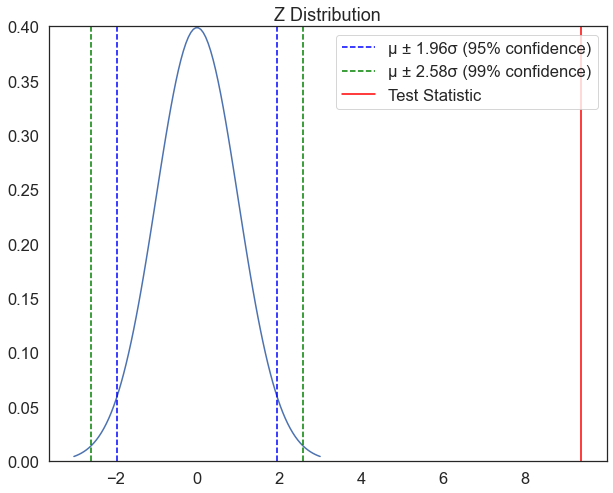
\includegraphics{notebooks/W06. Hypothesis Testing_files/figure-pdf/cell-13-output-1.png}

}

\end{figure}

Based on the plot above, can we reject the null hypothesis that there is
no difference in mean income between men and women?

\hypertarget{exercise-21}{%
\subsection{Exercise}\label{exercise-21}}

\begin{enumerate}
\def\labelenumi{\arabic{enumi}.}
\tightlist
\item
  From the main dataframe \texttt{df}, draw a sample of 500 white men.
  Using t-tests, investigate whether there are statistically significant
  discrepancies in pay between white men and other groups (note: it
  would be best to sample 500 people in each of those groups as well).
  Between what groups does there exist the most significant pay gap?
\item
  Some of this variation may be due to occupation. Compare income
  disparities between men and women within different occupations. Which
  occupation has the largest pay gap? which has the smallest?
\item
  \href{https://journals.sagepub.com/doi/abs/10.1177/0730888401028004005}{Research
  suggests} that within occupational groups, collective bargaining
  through union membership reduces pay gaps. Read the abstract of this
  article, and try to replicate the analysis using our dataset.
\end{enumerate}

\bookmarksetup{startatroot}

\hypertarget{regression}{%
\chapter{Regression}\label{regression}}

\hypertarget{workshop-7-open-in-colab-1}{%
\section[\emph{Workshop 7} ]{\texorpdfstring{\emph{Workshop 7}
\href{https://colab.research.google.com/github/oballinger/QM2/blob/main/notebooks/W07.\%20Linear\%20Regression.ipynb}{\protect
\includegraphics{index_files/mediabag/colab-badge.png}}}{Workshop 7 Open In Colab}}\label{workshop-7-open-in-colab-1}}

\hypertarget{aims-5}{%
\subsection{Aims:}\label{aims-5}}

In this workshop, we're going to be modeling the relationship between
education and income. More precisely, we're going to be looking at the
effect of increasing education on hourly wages using Ordinary Least
Squares regression. We're going to accomplish this in four steps:

\begin{enumerate}
\def\labelenumi{\arabic{enumi}.}
\tightlist
\item
  Summary Statistics

  \begin{itemize}
  \tightlist
  \item
    Table of Summary Statistics
  \end{itemize}
\item
  Visualisation

  \begin{itemize}
  \tightlist
  \item
    Exploratory Plots
  \end{itemize}
\item
  Assumptions

  \begin{itemize}
  \tightlist
  \item
    A. Independence
  \item
    B. Heteroscedasticity: Regression plots + Q-Q plot
  \item
    C. Multicollinearity: VIF + Correlation Matrix
  \end{itemize}
\item
  Regression

  \begin{itemize}
  \tightlist
  \item
    Regression Table
  \end{itemize}
\end{enumerate}

If you're conducting a regression, you must complete the steps above,
and produce each item indicated by a bullet point.

\hypertarget{getting-started-3}\NormalTok{matplotlib inline  }
\ImportTok{import}\NormalTok{ matplotlib.pyplot }\ImportTok{as}\NormalTok{ plt}
\ImportTok{import}\NormalTok{ statsmodels.api }\ImportTok{as}\NormalTok{ sm}
\ImportTok{from}\NormalTok{ math }\ImportTok{import}\NormalTok{ sqrt}
\ImportTok{from}\NormalTok{ numpy.random }\ImportTok{import}\NormalTok{ seed}
\ImportTok{from}\NormalTok{ numpy.random }\ImportTok{import}\NormalTok{ randn}
\ImportTok{from}\NormalTok{ numpy }\ImportTok{import}\NormalTok{ mean}
\ImportTok{from}\NormalTok{ scipy.stats }\ImportTok{import}\NormalTok{ sem}
\ImportTok{import}\NormalTok{ statistics }
\ImportTok{import}\NormalTok{ seaborn }\ImportTok{as}\NormalTok{ sns}
\ImportTok{from}\NormalTok{ IPython.display }\ImportTok{import}\NormalTok{ display, Math, Latex, display\_latex}
\ImportTok{import}\NormalTok{ plotly.express }\ImportTok{as}\NormalTok{ px}
\ImportTok{import}\NormalTok{ pylab}
\ImportTok{import}\NormalTok{ pandas }\ImportTok{as}\NormalTok{ pd}
\ImportTok{import}\NormalTok{ numpy }\ImportTok{as}\NormalTok{ np}
\CommentTok{\# make the plots (graphs) a little wider by default}
\NormalTok{pylab.rcParams[}\StringTok{\textquotesingle{}figure.figsize\textquotesingle{}}\NormalTok{] }\OperatorTok{=}\NormalTok{ (}\FloatTok{10.}\NormalTok{, }\FloatTok{8.}\NormalTok{)}
\NormalTok{sns.}\BuiltInTok{set}\NormalTok{(font\_scale}\OperatorTok{=}\FloatTok{1.5}\NormalTok{)}
\NormalTok{sns.set\_style(}\StringTok{"white"}\NormalTok{)}

\end{Highlighting}
\end{Shaded}

Now that I've imported the libraries I'm going to be using, I'm ready to
import the data:

\begin{Shaded}
\begin{Highlighting}[]
\NormalTok{df}\OperatorTok{=}\NormalTok{pd.read\_csv(}\StringTok{\textquotesingle{}https://storage.googleapis.com/qm2/wk7/cps.csv\textquotesingle{}}\NormalTok{)}
\NormalTok{df.head()}
\end{Highlighting}
\end{Shaded}

\begin{longtable}[]{@{}llllllllllll@{}}
\toprule\noalign{}
& year & state & age & sex & race & sch & ind & union & incwage &
realhrwage & occupation \\
\midrule\noalign{}
\endhead
\bottomrule\noalign{}
\endlastfoot
0 & 1990 & 36 & 58 & 1 & 3 & 12.0 & 871 & 0.0 & 14200.0 & 12.269874 &
Office and Admin Support \\
1 & 2009 & 5 & 28 & 1 & 1 & 12.0 & 8660 & 1.0 & 17680.0 & 8.635149 &
Office and Admin Support \\
2 & 1990 & 36 & 37 & 1 & 1 & 14.0 & 380 & 1.0 & 28000.0 & 21.169851 &
. \\
3 & 1990 & 6 & 34 & 1 & 1 & 18.0 & 740 & 1.0 & 27500.0 & 20.447746 &
Computer and Math Technicians \\
4 & 1981 & 51 & 38 & 1 & 4 & 13.0 & 798 & NaN & 17000.0 & 18.892282 &
Managers \\
\end{longtable}

Our dataframe has 10 columns:

\begin{enumerate}
\def\labelenumi{\arabic{enumi}.}
\tightlist
\item
  \emph{year}: Survey year
\item
  \emph{age}: the person's age
\item
  \emph{sex}: the person's sex

  \begin{itemize}
  \tightlist
  \item
    1=male
  \item
    2=female
  \end{itemize}
\item
  \emph{race}: the person's race

  \begin{itemize}
  \tightlist
  \item
    White non hispanic=1
  \item
    Black non hispanic=2
  \item
    Hispanic=3
  \item
    Other non hispanic=4)
  \end{itemize}
\item
  \emph{sch}: Educational attainment

  \begin{itemize}
  \tightlist
  \item
    None = 0,
  \item
    Grades 1-12 = 1-12
  \item
    Some University = 13,
  \item
    Associate's degree = 14,
  \item
    BA = 16
  \item
    Advanced Degree = 18
  \end{itemize}
\item
  \emph{union}: Union membership

  \begin{itemize}
  \tightlist
  \item
    N/A = 0,
  \item
    No union coverage = 1,
  \item
    Member of labor union=2,
  \item
    Covered by union but not a member=3
  \end{itemize}
\item
  \emph{incwage}: Wage and salary income
\item
  \emph{realhrwage}: Real Hourly Wage
\item
  \emph{occupation}: Occupation
\item
  \emph{ind}:
  \href{https://www.census.gov/naics/?58967?yearbck=2002}{industry code}
\item
  \emph{state}:
  \href{https://www.bls.gov/respondents/mwr/electronic-data-interchange/appendix-d-usps-state-abbreviations-and-fips-codes.htm}{FIPS
  code} denoting the state of residence.
\end{enumerate}

We'll begin, as we did with last week's workshop, by selecting the year
2013 in our data and making sure that all the variables that represent
categories are stored as categorical in python:

\begin{Shaded}
\begin{Highlighting}[]
\NormalTok{reg\_df}\OperatorTok{=}\NormalTok{df[df[}\StringTok{\textquotesingle{}year\textquotesingle{}}\NormalTok{]}\OperatorTok{==}\DecValTok{2013}\NormalTok{].drop([}\StringTok{\textquotesingle{}year\textquotesingle{}}\NormalTok{],axis}\OperatorTok{=}\DecValTok{1}\NormalTok{) }\CommentTok{\# filter the whole dataset to 2013 and drop year column}
\NormalTok{reg\_df[[}\StringTok{\textquotesingle{}race\textquotesingle{}}\NormalTok{,}\StringTok{\textquotesingle{}union\textquotesingle{}}\NormalTok{,}\StringTok{\textquotesingle{}sex\textquotesingle{}}\NormalTok{,}\StringTok{\textquotesingle{}occupation\textquotesingle{}}\NormalTok{,}\StringTok{\textquotesingle{}ind\textquotesingle{}}\NormalTok{,}\StringTok{\textquotesingle{}state\textquotesingle{}}\NormalTok{]]}\OperatorTok{=}\NormalTok{reg\_df[[}\StringTok{\textquotesingle{}race\textquotesingle{}}\NormalTok{,}\StringTok{\textquotesingle{}union\textquotesingle{}}\NormalTok{,}\StringTok{\textquotesingle{}sex\textquotesingle{}}\NormalTok{,}\StringTok{\textquotesingle{}occupation\textquotesingle{}}\NormalTok{, }\StringTok{\textquotesingle{}ind\textquotesingle{}}\NormalTok{,}\StringTok{\textquotesingle{}state\textquotesingle{}}\NormalTok{]].astype(}\StringTok{\textquotesingle{}category\textquotesingle{}}\NormalTok{) }\CommentTok{\# convert these columns to categorical}
\end{Highlighting}
\end{Shaded}

\hypertarget{summary-statistics-1}{%
\section{1. Summary Statistics}\label{summary-statistics-1}}

Once our data has been cleaned and all our variables are stored as the
appropriate type, we can start with the first step of any regression
project: creating a table of summary statistics. This is an important
part of the process, since it gives the reader a qualitative
understanding of your data before you analyze it. It also serves to
demonstrate that you've cleaned the data appropriately, and that the
measures of the variables make sense.

\begin{Shaded}
\begin{Highlighting}[]
\NormalTok{summary}\OperatorTok{=}\NormalTok{reg\_df.describe().}\BuiltInTok{round}\NormalTok{(}\DecValTok{2}\NormalTok{)  }\CommentTok{\# generate summary statistics, and round everything to 2 decimal degrees}
\NormalTok{summary}\OperatorTok{=}\NormalTok{summary.T }\CommentTok{\#.T transposes the table (rows become columns and vice versa)}
\NormalTok{summary}
\end{Highlighting}
\end{Shaded}

\begin{longtable}[]{@{}lllllllll@{}}
\toprule\noalign{}
& count & mean & std & min & 25\% & 50\% & 75\% & max \\
\midrule\noalign{}
\endhead
\bottomrule\noalign{}
\endlastfoot
age & 53790.0 & 42.91 & 10.56 & 25.00 & 34.00 & 43.00 & 51.00 & 64.0 \\
sch & 53790.0 & 13.93 & 2.74 & 0.00 & 12.00 & 13.00 & 16.00 & 18.0 \\
incwage & 53790.0 & 51821.86 & 60163.45 & 38.00 & 24000.00 & 40000.00 &
63000.00 & 1102999.0 \\
realhrwage & 53790.0 & 24.38 & 151.90 & 2.01 & 12.17 & 18.44 & 28.12 &
34760.8 \\
\end{longtable}

This table is already informative. I now know that the average person in
this dataset is 42 years old, has around 14 years of schooling, and
makes \$24/hour (or \$51,821/year). However, it's also useful to spot
potential errors in data entry that may warrant greater attention.

Notice the max value for real hourly wage. Despite the fact that those
in the top 75\% of earners make \$28.12/hour, someone is making \$34,760
per hour. Must be nice (or, may be a data entry error). Either way,
because regresisons are sensitive to this sort of outlier, we should
remove it. I've defined a function below that calculates the quartiles
and filters out observations that are more than three times as far away
form the top quartile as the top quartile is from the bottom one. This
was a somewhat arbitrary choice, but it allows me to be consistent if I
want to apply it to other variables. You could also just pick a cutoff
qualitatively and justify it (e.g.~``I will focus on those making up to
\$250k per year, since they represent the population i'm trying to
understand'').

\begin{Shaded}
\begin{Highlighting}[]
\KeywordTok{def}\NormalTok{ filter\_outliers(var):}
\NormalTok{    q1 }\OperatorTok{=}\NormalTok{ var.quantile(}\FloatTok{0.25}\NormalTok{) }\CommentTok{\# calculate the first quartile}
\NormalTok{    q3 }\OperatorTok{=}\NormalTok{ var.quantile(}\FloatTok{0.75}\NormalTok{) }\CommentTok{\# calculate the third quartile}
\NormalTok{    iqr }\OperatorTok{=}\NormalTok{ q3 }\OperatorTok{{-}}\NormalTok{ q1 }\CommentTok{\# calculate the interquartile range}
\NormalTok{    low }\OperatorTok{=}\NormalTok{ q1 }\OperatorTok{{-}} \DecValTok{3}\OperatorTok{*}\NormalTok{iqr }\CommentTok{\# calculate the lower bound}
\NormalTok{    high }\OperatorTok{=}\NormalTok{ q3 }\OperatorTok{+} \DecValTok{3}\OperatorTok{*}\NormalTok{iqr }\CommentTok{\# calculate the upper bound}
\NormalTok{    filtered }\OperatorTok{=}\NormalTok{ reg\_df[(var }\OperatorTok{\textgreater{}}\NormalTok{ low) }\OperatorTok{\&}\NormalTok{ (var }\OperatorTok{\textless{}}\NormalTok{ high)] }\CommentTok{\# filter  the values that are within the bounds}
\NormalTok{    dropped\_observations}\OperatorTok{=} \BuiltInTok{len}\NormalTok{(var)}\OperatorTok{{-}}\BuiltInTok{len}\NormalTok{(filtered) }\CommentTok{\# calculate the number of observations that were dropped}

    \BuiltInTok{print}\NormalTok{(}\StringTok{\textquotesingle{}Dropped }\SpecialCharTok{\{\}}\StringTok{ observations\textquotesingle{}}\NormalTok{.}\BuiltInTok{format}\NormalTok{(dropped\_observations))}
    \ControlFlowTok{return}\NormalTok{  filtered}

\NormalTok{reg\_df}\OperatorTok{=}\NormalTok{filter\_outliers(reg\_df[}\StringTok{\textquotesingle{}realhrwage\textquotesingle{}}\NormalTok{]) }\CommentTok{\# filter outliers from realhrwage}
\end{Highlighting}
\end{Shaded}

\begin{verbatim}
Dropped 1040 observations
\end{verbatim}

We can see that this operation dropped 1040 observations that had
extreme values in the ``realhrwage'' variable. Let's re-generate the
table of summary statistics and only keep four columns: count, mean,
standard deviaiton, minimum, and maximum.

\begin{Shaded}
\begin{Highlighting}[]
\NormalTok{summary}\OperatorTok{=}\NormalTok{reg\_df.describe().}\BuiltInTok{round}\NormalTok{(}\DecValTok{2}\NormalTok{).T}
\NormalTok{summary[[}\StringTok{\textquotesingle{}count\textquotesingle{}}\NormalTok{,}\StringTok{\textquotesingle{}mean\textquotesingle{}}\NormalTok{,}\StringTok{\textquotesingle{}std\textquotesingle{}}\NormalTok{,}\StringTok{\textquotesingle{}min\textquotesingle{}}\NormalTok{,}\StringTok{\textquotesingle{}max\textquotesingle{}}\NormalTok{]]}
\end{Highlighting}
\end{Shaded}

\begin{longtable}[]{@{}llllll@{}}
\toprule\noalign{}
& count & mean & std & min & max \\
\midrule\noalign{}
\endhead
\bottomrule\noalign{}
\endlastfoot
age & 52750.0 & 42.84 & 10.57 & 25.00 & 64.00 \\
sch & 52750.0 & 13.88 & 2.73 & 0.00 & 18.00 \\
incwage & 52750.0 & 46849.39 & 33376.96 & 38.00 & 353000.00 \\
realhrwage & 52750.0 & 21.59 & 13.03 & 2.01 & 75.81 \\
\end{longtable}

\hypertarget{visualization}{%
\section{2. Visualization}\label{visualization}}

The summary statistics table provides us with a good overview of some of
the variables we're interested in. However, you'll notice that it omits
many of the other variables in our dataset: the categorical ones. This
is because calculating the mean, standard deviation, etc. of something
like the ``occupation'' column doesn't really make sense. For that, we
turn to visualization.

\hypertarget{visualizing-the-distribution-of-categorical-variables}{%
\subsection{Visualizing the distribution of categorical
variables}\label{visualizing-the-distribution-of-categorical-variables}}

So far in this course we've been using a python library called
Matplotlib to make our visualizations, which we've been calling using
the `plt' alias. But this isn't the only one that is avaialble to us.
\href{https://seaborn.pydata.org/}{Seaborn} is another library that has
some cool plotting functions that are more geared towards statistical
analysis. We've already imported seaborn above, and we'll be calling it
using the alias ``sns''. We can use it in conjunction with matplotlib.

To get a sense of the distribution of our categorical variables, we'll
make some plots that count the number of observations in each category.
Let's start with the race category:

\begin{Shaded}
\begin{Highlighting}[]
\NormalTok{sns.countplot(data}\OperatorTok{=}\NormalTok{reg\_df, x}\OperatorTok{=}\StringTok{\textquotesingle{}race\textquotesingle{}}\NormalTok{) }\CommentTok{\# plot the union variable}

\NormalTok{plt.title(}\StringTok{\textquotesingle{}Race\textquotesingle{}}\NormalTok{) }\CommentTok{\# add a title}
\NormalTok{plt.xlabel(}\StringTok{\textquotesingle{}\textquotesingle{}}\NormalTok{) }\CommentTok{\# remove the x axis label}
\NormalTok{plt.xticks(ticks}\OperatorTok{=}\NormalTok{[}\DecValTok{0}\NormalTok{,}\DecValTok{1}\NormalTok{,}\DecValTok{2}\NormalTok{,}\DecValTok{3}\NormalTok{],labels}\OperatorTok{=}\NormalTok{[}\StringTok{\textquotesingle{}White\textquotesingle{}}\NormalTok{, }\StringTok{\textquotesingle{}Black\textquotesingle{}}\NormalTok{,}\StringTok{\textquotesingle{}Hispanic\textquotesingle{}}\NormalTok{,}\StringTok{\textquotesingle{}Other\textquotesingle{}}\NormalTok{]) }\CommentTok{\# replace the x axis labels with more descriptive labels}
\NormalTok{plt.show() }\CommentTok{\# show the plot}
\end{Highlighting}
\end{Shaded}

\begin{figure}[H]

{\centering 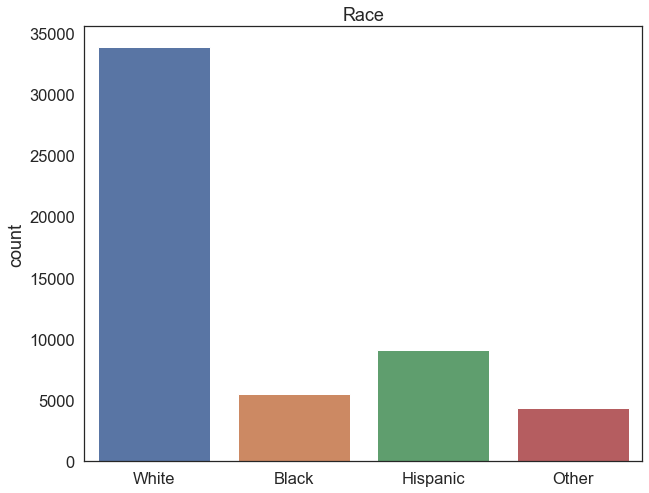
\includegraphics{notebooks/W07. Linear Regression_files/figure-pdf/cell-8-output-1.png}

}

\end{figure}

\hypertarget{exercise-22}{%
\subsection{Exercise}\label{exercise-22}}

\begin{enumerate}
\def\labelenumi{\arabic{enumi}.}
\tightlist
\item
  Generate an equivalent plot for the other categorical columns
\item
  What is the most common industry code, and what does it correpsond to?
\end{enumerate}

\hypertarget{assumptions}{%
\section{3. Assumptions}\label{assumptions}}

Once you've generated summary statistics for your continuous variables
and exploratory plots for the categorical ones, it's time to start
thinking about the relationships \emph{between} the variables. Today,
we're going to be modeling a linear relationship between income and
years of schooling, by means of a \textbf{linear regression}. But before
we do that, we need to check a couple things-- all statistical tests
have a number of assumptions that must be satisfied in order to yield
robust results. Before we run a regression, we must check that the
assumptions in this case are satisfied. There are four main ones:

\begin{verbatim}
A. Indepdendence 
B. Homoscedasticity
C. Multicollinearity 
\end{verbatim}

Let's go through them one by one.

\hypertarget{a.-independence}{%
\subsection{A. Independence}\label{a.-independence}}

\textbf{\texttt{Linear\ regression\ assumes\ that\ measurements\ for\ each\ sample\ subject\ are\ in\ no\ way\ influenced\ by\ or\ related\ to\ the\ measurements\ of\ other\ subjects.}}

Though in the full CPS dataset we have repeat observations of the same
individual over time, we've only been analyzing one year's worth of
data, so we satisfy the independence assumption. If we ran a regression
on the full sample over multiple years, \emph{this would violate the
independence assumption}. It's very possible to run a regression with
repeat observations of the same units (people, places, etc.) over time,
but you need to use a special type of regression called a \textbf{panel
regression}. More on that next week.

\hypertarget{b.-homoscedasticity}{%
\subsection{B. Homoscedasticity}\label{b.-homoscedasticity}}

\textbf{\texttt{Linear\ regression\ assumes\ that\ the\ variance\ of\ residuals\ is\ the\ same\ for\ any\ value\ of\ x,\ and\ that\ residuals\ are\ normally\ distributed\ with\ a\ mean\ of\ 0.}}

This is a complicated way of saying your regression line should fit
consistently across the full range of \(x\) values. If there are really
small residuals (i.e., all the data points are close to the line) for
low values of \(x\), but larger residuals for high values of \(x\), the
regression is not performing well-- we wouldn't have the same confidence
in our predictions at different values of \(x\). Similarly, if all the
residuals are on one side of the regression line in different parts of
the \(x\) range, the model will consistently over/underestimate in those
regions. When the variance of residuals from a regression model are
inconsistent, we have \textbf{\texttt{Heteroscedasticity}}.

We can explore potential heteroscedasticity by visually inspecting a
regression plot. In our case, we're primarily interested in the
relationship between years of schooling and hourly wages, so we'll be
plotting these variables against eachother. \texttt{sns.jointplot()}
lets us create a plot with four components which can help us diagnose
potential heteroscedasticity:

\begin{itemize}
\tightlist
\item
  The main plot is a scatterplot between hourly wages on the y axis, and
  years of schooling on the x axis.
\item
  A regression line overlaid on this plot lets us see the relationship
  between our model and the underlying data
\item
  A histogram to the right of the plot shows the distribution of the
  hourly wages variable, which is heavily skewed.
\item
  A histogram above the plot shows the distribution of the years of
  schooling variable, which has an almost bimodal form.
\end{itemize}

\begin{Shaded}
\begin{Highlighting}[]
\NormalTok{sns.jointplot(data}\OperatorTok{=}\NormalTok{reg\_df, }\CommentTok{\# plot a scatterplot with a regression line and two histograms}
\NormalTok{                x}\OperatorTok{=}\StringTok{\textquotesingle{}sch\textquotesingle{}}\NormalTok{, }\CommentTok{\# set the x axis to be the years of schooling}
\NormalTok{                y}\OperatorTok{=}\StringTok{\textquotesingle{}realhrwage\textquotesingle{}}\NormalTok{, }\CommentTok{\# set the y axis to be the hourly wage}
\NormalTok{                kind}\OperatorTok{=}\StringTok{"reg"}\NormalTok{,  }\CommentTok{\# set the kind of plot to be a regression plot}
\NormalTok{                scatter\_kws}\OperatorTok{=}\BuiltInTok{dict}\NormalTok{(alpha}\OperatorTok{=}\FloatTok{0.1}\NormalTok{), }\CommentTok{\# set the transparency of the points to be 0.1 (10\%)}
\NormalTok{                line\_kws}\OperatorTok{=}\BuiltInTok{dict}\NormalTok{(color}\OperatorTok{=}\StringTok{\textquotesingle{}red\textquotesingle{}}\NormalTok{), }\CommentTok{\# set the color of the regression line to red}
\NormalTok{                height}\OperatorTok{=}\DecValTok{10}\NormalTok{) }\CommentTok{\# set the height of the plot to be 10 inches }

\NormalTok{plt.xlabel(}\StringTok{\textquotesingle{}Years of Schooling\textquotesingle{}}\NormalTok{) }\CommentTok{\# add a label to the x axis}
\NormalTok{plt.ylabel(}\StringTok{\textquotesingle{}Hourly Wage\textquotesingle{}}\NormalTok{) }\CommentTok{\# add a label to the y axis}
\end{Highlighting}
\end{Shaded}

\begin{verbatim}
Text(53.625, 0.5, 'Hourly Wage')
\end{verbatim}

\begin{figure}[H]

{\centering \includegraphics{notebooks/W07. Linear Regression_files/figure-pdf/cell-9-output-2.png}

}

\end{figure}

The plot above is cause for concern. From 0 to 5 years of schooling the
model has underestimated hourly wages for every single observation.
Conversely, at the far right tip of the regression line, we can see that
the model \emph{overestimates} income for many individuals with 18 years
of schooling. This gives us reason to suspect that there may be
asymmetry in the residuals of our model (heteroscedasticity). We're
going to fix this in the Exension section below. But for now, let's
proceed.

\hypertarget{c.-multicollinearity}{%
\subsection{C. Multicollinearity}\label{c.-multicollinearity}}

\textbf{\texttt{Multicollinearity\ emerges\ when\ two\ or\ more\ independent\ variables\ which\ are\ highly\ correlated\ are\ included\ in\ a\ model.}}
A key goal of regression analysis is to isolate the relationship between
each independent variable and the dependent variable. The interpretation
of a regression coefficient is that it represents the mean change in the
dependent variable for each 1 unit change in an independent variable
when you hold all of the other independent variables constant.

The idea is that you can change the value of one independent variable
and not the others. However, when independent variables are correlated,
it indicates that changes in one variable are associated with shifts in
another variable. The stronger the correlation, the more difficult it is
to change one variable without changing another. See this
\href{https://statisticsbyjim.com/regression/multicollinearity-in-regression-analysis/}{blog
post} for a thorough explanation.

One way of visually exporing multicollinearity is through a correlation
matrix:

\begin{Shaded}
\begin{Highlighting}[]
\NormalTok{sns.heatmap(reg\_df[[}\StringTok{\textquotesingle{}incwage\textquotesingle{}}\NormalTok{,}\StringTok{\textquotesingle{}realhrwage\textquotesingle{}}\NormalTok{,}\StringTok{\textquotesingle{}age\textquotesingle{}}\NormalTok{,}\StringTok{\textquotesingle{}sch\textquotesingle{}}\NormalTok{]].corr(), }\CommentTok{\# plot a correlation matrix }
\NormalTok{            annot}\OperatorTok{=}\VariableTok{True}\NormalTok{, }\CommentTok{\# show the correlation values on the plot}
\NormalTok{            fmt}\OperatorTok{=}\StringTok{".2f"}\NormalTok{, }\CommentTok{\# set the format of the correlation values to be two decimal places}
\NormalTok{            cmap}\OperatorTok{=}\StringTok{\textquotesingle{}coolwarm\textquotesingle{}}\NormalTok{) }\CommentTok{\# set the color palette to be coolwarm (blue for negative correlations, red for positive correlations)}

\NormalTok{plt.title(}\StringTok{\textquotesingle{}Correlation Matrix\textquotesingle{}}\NormalTok{) }\CommentTok{\# add a title}
\end{Highlighting}
\end{Shaded}

\begin{verbatim}
Text(0.5, 1.0, 'Correlation Matrix')
\end{verbatim}

\begin{figure}[H]

{\centering \includegraphics{notebooks/W07. Linear Regression_files/figure-pdf/cell-10-output-2.png}

}

\end{figure}

This matrix has each of the continuous variables in \texttt{reg\_df} on
both axes. Each cell denotes the correlation between the corresponding
variables. Naturally, on the diagonal we have a series of perfect
correlations (1.00), as each variable is perfectly correlated with
itself. \texttt{incwage} (annual salary) and \texttt{realhrwage} (hourly
wage) are highly correlated with each other, which makes a lot of sense.
This isn't a concern for multicollinearity, though, since
\texttt{realhrwage} will be our dependent variable. This type of
correlation matrix is also a good way of conducting exploratory data
analysis-- we can already see that the next-highest set of correlations
is between years of schooling and both hourly wages and annual salary.

Though a very high correlagtion coefficient between independent
variables is a cause for concern, the formal way of dealing with
muticollinearity is through the use of the
\textbf{\texttt{Variance\ Inflation\ Factor\ (VIF)}}. VIF is the ratio
of the variance in a model with multiple predictors by the variance of a
model with a single predictor:

\[\large VIF_j=\frac{1}{1-R_{j}^{2}}\]

VIFs start at 1 and have no upper limit. A value of 1 indicates that
there is no correlation between this independent variable and any
others. VIFs between 1 and 5 suggest that there is a moderate
correlation, but it is not severe enough to warrant corrective measures.
VIFs greater than 5 represent critical levels of multicollinearity where
the coefficients are poorly estimated, and the p-values are
questionable. More explanation of the theory can be found
\href{https://en.wikipedia.org/wiki/Variance_inflation_factor}{here}.

Below is a function that calculates VIF for each independent variable in
a dataframe, and drops them if they exceed a threshold (set to 5).

\begin{Shaded}
\begin{Highlighting}[]
\CommentTok{\# calculating VIF}
\CommentTok{\# This function is amended from: https://stackoverflow.com/a/51329496/4667568}

\ImportTok{from}\NormalTok{ statsmodels.stats.outliers\_influence }\ImportTok{import}\NormalTok{ variance\_inflation\_factor }
\ImportTok{from}\NormalTok{ statsmodels.tools.tools }\ImportTok{import}\NormalTok{ add\_constant}

\KeywordTok{def}\NormalTok{ drop\_column\_using\_vif\_(df, list\_var\_not\_to\_remove}\OperatorTok{=}\VariableTok{None}\NormalTok{, thresh}\OperatorTok{=}\DecValTok{5}\NormalTok{):}
    \CommentTok{\textquotesingle{}\textquotesingle{}\textquotesingle{}}
\CommentTok{    Calculates VIF each feature in a pandas dataframe, and repeatedly drop the columns with the highest VIF}
\CommentTok{    A constant must be added to variance\_inflation\_factor or the results will be incorrect}

\CommentTok{    :param df: the pandas dataframe containing only the predictor features, not the response variable}
\CommentTok{    :param list\_var\_not\_to\_remove: the list of variables that should not be removed even though it has a high VIF. For example, dummy (or indicator) variables represent a categorical variable with three or more categories.}
\CommentTok{    :param thresh: the max VIF value before the feature is removed from the dataframe}
\CommentTok{    :return: dataframe with multicollinear features removed}
\CommentTok{    \textquotesingle{}\textquotesingle{}\textquotesingle{}}
    \ControlFlowTok{while} \VariableTok{True}\NormalTok{:}
        \CommentTok{\# adding a constatnt item to the data}
\NormalTok{        df\_with\_const }\OperatorTok{=}\NormalTok{ add\_constant(df)}

\NormalTok{        vif\_df }\OperatorTok{=}\NormalTok{ pd.Series([variance\_inflation\_factor(df\_with\_const.values, i) }
               \ControlFlowTok{for}\NormalTok{ i }\KeywordTok{in} \BuiltInTok{range}\NormalTok{(df\_with\_const.shape[}\DecValTok{1}\NormalTok{])], name}\OperatorTok{=} \StringTok{"VIF"}\NormalTok{,}
\NormalTok{              index}\OperatorTok{=}\NormalTok{df\_with\_const.columns).to\_frame()}

        \CommentTok{\# drop the const as const should not be removed}
\NormalTok{        vif\_df }\OperatorTok{=}\NormalTok{ vif\_df.drop(}\StringTok{\textquotesingle{}const\textquotesingle{}}\NormalTok{)}
        
        \CommentTok{\# drop the variables that should not be removed}
        \ControlFlowTok{if}\NormalTok{ list\_var\_not\_to\_remove }\KeywordTok{is} \KeywordTok{not} \VariableTok{None}\NormalTok{:}
\NormalTok{            vif\_df }\OperatorTok{=}\NormalTok{ vif\_df.drop(list\_var\_not\_to\_remove)}
            
        \BuiltInTok{print}\NormalTok{(}\StringTok{\textquotesingle{}Max VIF:\textquotesingle{}}\NormalTok{, vif\_df.VIF.}\BuiltInTok{max}\NormalTok{())}
        
        \CommentTok{\# if the largest VIF is above the thresh, remove a variable with the largest VIF}
        \ControlFlowTok{if}\NormalTok{ vif\_df.VIF.}\BuiltInTok{max}\NormalTok{() }\OperatorTok{\textgreater{}}\NormalTok{ thresh:}
            \CommentTok{\# If there are multiple variables with the maximum VIF, choose the first one}
\NormalTok{            index\_to\_drop }\OperatorTok{=}\NormalTok{ vif\_df.index[vif\_df.VIF }\OperatorTok{==}\NormalTok{ vif\_df.VIF.}\BuiltInTok{max}\NormalTok{()].tolist()[}\DecValTok{0}\NormalTok{]}
            \BuiltInTok{print}\NormalTok{(}\StringTok{\textquotesingle{}Dropping: }\SpecialCharTok{\{\}}\StringTok{\textquotesingle{}}\NormalTok{.}\BuiltInTok{format}\NormalTok{(index\_to\_drop))}
\NormalTok{            df }\OperatorTok{=}\NormalTok{ df.drop(columns }\OperatorTok{=}\NormalTok{ index\_to\_drop)}
        \ControlFlowTok{else}\NormalTok{:}
            \CommentTok{\# No VIF is above threshold. Exit the loop}
            \ControlFlowTok{break}

    \ControlFlowTok{return}\NormalTok{ df}
\end{Highlighting}
\end{Shaded}

Now we can implement this on our dataset:

\begin{Shaded}
\begin{Highlighting}[]
\NormalTok{ind\_vars}\OperatorTok{=}\NormalTok{[}\StringTok{\textquotesingle{}sex\textquotesingle{}}\NormalTok{,}\StringTok{\textquotesingle{}age\textquotesingle{}}\NormalTok{,}\StringTok{\textquotesingle{}sch\textquotesingle{}}\NormalTok{, }\StringTok{\textquotesingle{}union\textquotesingle{}}\NormalTok{,}\StringTok{\textquotesingle{}race\textquotesingle{}}\NormalTok{]}

\NormalTok{vif }\OperatorTok{=}\NormalTok{ drop\_column\_using\_vif\_(reg\_df[ind\_vars], thresh}\OperatorTok{=}\DecValTok{5}\NormalTok{)}
\BuiltInTok{print}\NormalTok{(}\StringTok{"The columns remaining after VIF selection are:"}\NormalTok{)}
\BuiltInTok{print}\NormalTok{(vif.columns)}
\end{Highlighting}
\end{Shaded}

\begin{verbatim}
Max VIF: 1.0471509029112354
The columns remaining after VIF selection are:
Index(['sex', 'age', 'sch', 'union', 'race'], dtype='object')
\end{verbatim}

The maximum VIF value encountered was 1.04-- well within the acceptable
range. Accordingly, the function hasn't dropped any of the independent
variables in our dataset.

Having explored our data through visualizations and summary statistics,
and checked the assumptions of linear regression, we're now ready to
begin building a model.

\hypertarget{regression-1}{%
\section{4. Regression}\label{regression-1}}

Remember, the Ordinary Least Squares (OLS) regression seeks to find a
straight line that best describes the relationship between two
variables:

\[y= \beta_0 + \beta_1x+\epsilon \]

In our case, we're trying to predict hourly income-- this is our
\textbf{dependent variable}, and there can be only one per regression.
The variable we're using to predict hourly income is years of schooling,
which is our \textbf{independent variable}. We can have multiple of
these per regression. As such, the regression equation in our scenario
looks like this:

\[Hourly\ Income= \beta_0 + \beta_1 \times Years\ of\ Schooling +\epsilon \]

Because the regression model will estimate the parameters
\(\beta_0, \beta_1\) and \(\epsilon\), we just need to supply python
with \(x\) and \(y\); We can do so by passing
\texttt{realhrwage\ \textasciitilde{}\ \ sch} to the \texttt{ols()}
function from statsmodels. This will run a regression of the form
specified above, which we will store in an variable called
\texttt{model}. We can get the output from this model using
\texttt{model.summary()}:

\begin{Shaded}
\begin{Highlighting}[]
\ImportTok{from}\NormalTok{ statsmodels.formula.api }\ImportTok{import}\NormalTok{ ols}
\ImportTok{from}\NormalTok{ statsmodels.iolib.summary2 }\ImportTok{import}\NormalTok{ summary\_col}

\NormalTok{model}\OperatorTok{=}\NormalTok{ ols(}\StringTok{\textquotesingle{}realhrwage \textasciitilde{}  sch\textquotesingle{}}\NormalTok{, data}\OperatorTok{=}\NormalTok{reg\_df).fit() }\CommentTok{\# fit the model}
\BuiltInTok{print}\NormalTok{(model.summary()) }\CommentTok{\# print the summary}
\end{Highlighting}
\end{Shaded}

\begin{verbatim}
                            OLS Regression Results                            
==============================================================================
Dep. Variable:             realhrwage   R-squared:                       0.181
Model:                            OLS   Adj. R-squared:                  0.181
Method:                 Least Squares   F-statistic:                 1.164e+04
Date:                Fri, 01 Dec 2023   Prob (F-statistic):               0.00
Time:                        09:05:19   Log-Likelihood:            -2.0503e+05
No. Observations:               52750   AIC:                         4.101e+05
Df Residuals:                   52748   BIC:                         4.101e+05
Df Model:                           1                                         
Covariance Type:            nonrobust                                         
==============================================================================
                 coef    std err          t      P>|t|      [0.025      0.975]
------------------------------------------------------------------------------
Intercept     -6.6246      0.266    -24.858      0.000      -7.147      -6.102
sch            2.0327      0.019    107.887      0.000       1.996       2.070
==============================================================================
Omnibus:                    10230.138   Durbin-Watson:                   1.900
Prob(Omnibus):                  0.000   Jarque-Bera (JB):            19817.137
Skew:                           1.187   Prob(JB):                         0.00
Kurtosis:                       4.838   Cond. No.                         73.7
==============================================================================

Notes:
[1] Standard Errors assume that the covariance matrix of the errors is correctly specified.
\end{verbatim}

There's a lot going on in the regression output above. If you want a
more detailed explanation of what each part means, check out this
\href{https://medium.com/swlh/interpreting-linear-regression-through-statsmodels-summary-4796d359035a}{blog
post}. In practice, we only need to focus on a couple parts of this
output:

\begin{itemize}
\tightlist
\item
  \texttt{R-squared}: This value tells the proportion of the variation
  in our dependent variable (realhrwage) that is explained by the model
  we fit. In this case we can interpret it as follows:

  \begin{itemize}
  \tightlist
  \item
    \textbf{18.1\% of the variation in hourly wages can be explained by
    this regresion model}
  \end{itemize}
\item
  \texttt{coef}: These are our \(\beta\) estimates; it is the slope of
  the regression line that describes the relationship between a given
  independent variable (sch) and the dependent variable (realhrwage).
  There are two coefficients listed under this

  \begin{itemize}
  \tightlist
  \item
    \texttt{sch}: This is \(\beta_1\), the slope coefficient on the
    years of schooling variable. It tells us the change in \(y\) that
    results from a 1-unit increase in \(x\). In robotic terms, we can
    interpret it as follows:

    \begin{itemize}
    \tightlist
    \item
      \textbf{A 1 unit increase in \texttt{sch} leads to a 2.0327
      increase in \texttt{realhrwage}}. But we are not robots, and both
      of these variables are in units that we can interpret in plain
      english. Here's a more natural interpretation:
    \item
      \textbf{On average, every additional year of schooling is
      associated with a \$2.03 increase in hourly wages.}
    \end{itemize}
  \item
    \texttt{Intercept}: This is \(\beta_0\). It tells us the value of
    \(y\) when all of the independent variables in the model are held at
    0. In this case, it can be interpreted as

    \begin{itemize}
    \tightlist
    \item
      \textbf{According to our model, a person with 0 years of schooling
      is predicted to earn -\$6.62 per hour}
    \item
      Naturally, this is a nonsensical prediction. There are no jobs
      that pay negative wages. We'll examine why this is happening in
      the next section, when we look into the assumptions of linear
      regression.
    \end{itemize}
  \end{itemize}
\item
  \texttt{P\textgreater{}\textbar{}t\textbar{}}: this is known as the
  ``p-value'', and is the main measure of statistical significance.
  \textbf{A p-value denotes the probability of obtaining a result at
  least as extreme as the one observed, assuming that the null
  hypothesis is true}. In the case of a regression, the null hypothesis
  is that there is no relationship between our variables-- increasing
  \(x\) has no effect on \(y\). In other words, that the regression line
  is flat: \(\beta_1=0\) . A p-value of 0.05 means that the coefficient
  is statistically significant at the 5\% level. In our case, the
  p-value is 0.000 (note: this doesn't mean it's equal to zero, just
  very very small), and we can therefore reject the null hypothesis that
  \(\beta_1=0\) at the 1\% confidence level. However, this isn't the end
  of the story-- remember our weird negative intercept, and the fact
  that our model explains less than 20\% of the variation in hourly
  wages (\(R^2=0.181\)). For a good overview of what exactly a p-value
  is, and why we should be cautious when interpreting them, see this
  \href{https://www.ncbi.nlm.nih.gov/pmc/articles/PMC6532382/}{journal
  article}.
\end{itemize}

\hypertarget{categorical-variables}{%
\subsection{Categorical Variables}\label{categorical-variables}}

The results of our first regression seem to show that the more education
a person has, the higher their hourly wage. This makes intuitive sense,
but it's probably not the whole picture. We may also suspect that older
people earn more, since they have more experience and are more senior.
We've also seen i previous classes that there are significant
disparities in income. Considering we have data on all these variables,
we can set up the following model:

\[Hourly\ Income= \beta_0 + \beta_1 \times Years\ of\ Schooling + \beta_2 \times Age + \beta_3 \times Sex +\epsilon \]

When we convert this equation into the python equivalent, it will look
like this:

\texttt{realhrwage\ \textasciitilde{}\ \ sch\ +\ age\ +\ C(sex)}

Notice that for the sex variable is put within \texttt{C()}. This is how
we indicate that the variable in question is categorical, and that it
should be treated differently. Unlike a continuous variable, we're not
interested in the change in \(y\) that results from a 1 unit increase in
\(x\), since our units have no meaningful order. Instead, we'll have to
pick one of the categories (called a \textbf{base
category}/\textbf{reference category}), and compare each of the other
categories in that variable against this one. You can specify the base
category explicitly (for example
\texttt{realhrwage\ \textasciitilde{}\ \ sch\ +\ age\ +\ C(sex,\ Treatment(reference=2))}
makes women the base category), or python will pick one for you. As
such, for a categorical variable with \(n\) categories, we get \(n-1\)
coefficeints which denote the change in \(y\) associated with membership
of a given category compared to the base category. For example, if we
have a categorical variable with three levels \(a, b, c\) where \(a\) is
the base category, we would get \emph{two} coefficients: \(\beta_1 b\)
and \(\beta_2 c\). Then we would interpret the resulting coefficient as

\begin{itemize}
\tightlist
\item
  ``Compared to category \(a\), membership of category \(b\) is
  associated with a \(\beta_1\) change in \(y\).''
\item
  ``Compared to category \(a\), membership of category \(c\) is
  associated with a \(\beta_2\) change in \(y\).''
\end{itemize}

Let's see what this looks like in our regression output:

\begin{Shaded}
\begin{Highlighting}[]
\NormalTok{model }\OperatorTok{=}\NormalTok{ ols(}\StringTok{\textquotesingle{}realhrwage \textasciitilde{}  sch + age + C(sex)\textquotesingle{}}\NormalTok{, data}\OperatorTok{=}\NormalTok{reg\_df).fit() }
\BuiltInTok{print}\NormalTok{(model.summary())}
\end{Highlighting}
\end{Shaded}

\begin{verbatim}
                            OLS Regression Results                            
==============================================================================
Dep. Variable:             realhrwage   R-squared:                       0.239
Model:                            OLS   Adj. R-squared:                  0.239
Method:                 Least Squares   F-statistic:                     5514.
Date:                Fri, 01 Dec 2023   Prob (F-statistic):               0.00
Time:                        09:05:19   Log-Likelihood:            -2.0310e+05
No. Observations:               52750   AIC:                         4.062e+05
Df Residuals:                   52746   BIC:                         4.062e+05
Df Model:                           3                                         
Covariance Type:            nonrobust                                         
===============================================================================
                  coef    std err          t      P>|t|      [0.025      0.975]
-------------------------------------------------------------------------------
Intercept     -12.6722      0.330    -38.392      0.000     -13.319     -12.025
C(sex)[T.2]    -5.2692      0.099    -52.967      0.000      -5.464      -5.074
sch             2.1343      0.018    116.995      0.000       2.098       2.170
age             0.1695      0.005     36.164      0.000       0.160       0.179
==============================================================================
Omnibus:                     9831.824   Durbin-Watson:                   1.995
Prob(Omnibus):                  0.000   Jarque-Bera (JB):            19481.335
Skew:                           1.131   Prob(JB):                         0.00
Kurtosis:                       4.935   Cond. No.                         308.
==============================================================================

Notes:
[1] Standard Errors assume that the covariance matrix of the errors is correctly specified.
\end{verbatim}

We now have 4 coefficients. In general, we don't always have to
interpret the Intercept coefficient. It's not really that meaningful in
this case, since now it denotes the predicted hourly income of someone
who is male, has 0 years of schooling, and is 0 years old. It's good to
keep it in mind as a sense check, though. The rest of the coefficients
can be interpreted as follows:

\begin{itemize}
\tightlist
\item
  \texttt{C(sex){[}T.2{]}}: On average, women earn \$5.2 less per hour
  than men.

  \begin{itemize}
  \tightlist
  \item
    {[}T.2{]} in this line denotes the category in this variable
    associated with the given coefficient. So this is telling us that
    what is being shown is the coefficient associated with membership of
    category 2 in the sex variable; based on the description of the
    variables above, we know that sex=1 indicates men, and sex=2
    indicates women. Naturally, we don't see a coefficient for
    \texttt{C(sex){[}T.1{]}}, because this is the \emph{base category}.
  \end{itemize}
\item
  \texttt{sch}: Every additional year of schooling is associated with a
  \$2.13 increase in hourly income
\item
  \texttt{age}: Every additional year of age is associated with a \$0.16
  increase in hourly income
\end{itemize}

\hypertarget{exercise-23}{%
\subsection{Exercise}\label{exercise-23}}

\begin{enumerate}
\def\labelenumi{\arabic{enumi}.}
\tightlist
\item
  Estimate a regression of the following form and store the results in a
  variable called \textbf{model1}:
\end{enumerate}

\[Hourly\ Income= \beta_0 + \beta_1 \times Years\ of\ Schooling + \beta_2 \times Age + \beta_3 \times Sex + \beta_4 \times Union\ Membership + \beta_5 \times Race +\epsilon \]

\begin{enumerate}
\def\labelenumi{\arabic{enumi}.}
\setcounter{enumi}{1}
\tightlist
\item
  Intepret each of the coefficients appropriately. Make note of the
  statistical significance of each result, and comment on the overall
  fit of the model.
\end{enumerate}

\hypertarget{creating-a-regression-table}{%
\subsection{Creating a Regression
Table}\label{creating-a-regression-table}}

Now that we've got a good sense of how regressions work and how to
interpret them, we need to communicate these results properly. Many of
you have probably read journal articles in which regression results are
reported, but I doubt you've ever seen the output of
\texttt{model.summary()} copied and pasted in the text of an article.
Instead, these results are reported following a fairly standardized
convention: a regression table. It picks out the components of the model
summary that we're interested in, and formats them in a consistent and
easy-to-interpret way. Luckly, the statsmodels package has a function
called \texttt{summary\_col} that takes a fitted model and formats it
for us automatically; we just need to tweak a few options.

In the example below, i'm going to run two regressions; one in which i
filter the data to only include people from California, and another for
people in Mississippi (the richest and poorest states, respectively), to
see if the relationship between wages, sex, age, and schooling differ
geographically. I'm then going to create a regression table in which
each column is a different regression model, and row will contain the
coefficient for a given independent variable with the standard error in
parentheses underneath and the level of statistical significance (i.e.,
size of the p-value) denotes by stars such that: * p\textless0.05, **
p\textless0.01, *** p\textless0.001.

\begin{Shaded}
\begin{Highlighting}[]
\NormalTok{california }\OperatorTok{=}\NormalTok{ ols(}\StringTok{\textquotesingle{}realhrwage \textasciitilde{}  sch + age + C(sex)\textquotesingle{}}\NormalTok{, data}\OperatorTok{=}\NormalTok{reg\_df[reg\_df[}\StringTok{\textquotesingle{}state\textquotesingle{}}\NormalTok{]}\OperatorTok{==}\DecValTok{6}\NormalTok{]).fit()  }\CommentTok{\# fit a model to california{-}{-} i\textquotesingle{}m filtering the data using the FIPS code for california, which is 6}
\NormalTok{mississippi }\OperatorTok{=}\NormalTok{ ols(}\StringTok{\textquotesingle{}realhrwage \textasciitilde{}  sch + age + C(sex)\textquotesingle{}}\NormalTok{, data}\OperatorTok{=}\NormalTok{reg\_df[reg\_df[}\StringTok{\textquotesingle{}state\textquotesingle{}}\NormalTok{]}\OperatorTok{==}\DecValTok{28}\NormalTok{]).fit()  }\CommentTok{\# same thing for mississippi (FIPS code 28)}

\NormalTok{table}\OperatorTok{=}\NormalTok{summary\_col( }\CommentTok{\# create a regression table }
\NormalTok{    [california,mississippi], }\CommentTok{\# pass the models to the summary\_col function}
\NormalTok{    stars}\OperatorTok{=}\VariableTok{True}\NormalTok{, }\CommentTok{\# add stars denoting the p{-}values of the coefficient to the table; * p\textless{}0.05, ** p\textless{}0.01, *** p\textless{}0.001}
\NormalTok{    float\_format}\OperatorTok{=}\StringTok{\textquotesingle{}}\SpecialCharTok{\%0.3f}\StringTok{\textquotesingle{}}\NormalTok{, }\CommentTok{\# set the decimal places to 3}
\NormalTok{    model\_names}\OperatorTok{=}\NormalTok{[}\StringTok{\textquotesingle{}California\textquotesingle{}}\NormalTok{,}\StringTok{\textquotesingle{}Mississippi\textquotesingle{}}\NormalTok{], }\CommentTok{\# set the name of the model}
\NormalTok{    info\_dict }\OperatorTok{=}\NormalTok{ \{}\StringTok{"N"}\NormalTok{:}\KeywordTok{lambda}\NormalTok{ x: }\StringTok{"}\SpecialCharTok{\{0:d\}}\StringTok{"}\NormalTok{.}\BuiltInTok{format}\NormalTok{(}\BuiltInTok{int}\NormalTok{(x.nobs))\}) }\CommentTok{\# add the number of observations to the table}

\BuiltInTok{print}\NormalTok{(table)}
\end{Highlighting}
\end{Shaded}

\begin{verbatim}

=====================================
               California Mississippi
-------------------------------------
Intercept      -12.136*** -10.111*** 
               (1.030)    (3.497)    
C(sex)[T.2]    -5.154***  -4.980***  
               (0.350)    (0.924)    
sch            2.096***   1.850***   
               (0.053)    (0.205)    
age            0.217***   0.115**    
               (0.017)    (0.045)    
R-squared      0.262      0.199      
R-squared Adj. 0.262      0.193      
N              5079       430        
=====================================
Standard errors in parentheses.
* p<.1, ** p<.05, ***p<.01
\end{verbatim}

This layout lets us clearly explore our regresison results. This lets us
clearly compare the coefficients of the same variable in different
models. For example, we can see that men tend to earn \$5.15 more per
hour than women in California, but just \$4.98 more per hour in
Mississippi, and both of these results are statistically significant at
the 1\% level. This suggests that the wage gap is actually somewhat
higher in California! Why might this be?

\hypertarget{exercise-24}{%
\subsection{Exercise}\label{exercise-24}}

\[ Hourly\ Income= \beta_0 + \beta_1 \times Years\ of\ Schooling + \beta_2 \times Age + \beta_3 \times Sex + \beta_4 \times Union\ Membership + \beta_5 \times Race +\epsilon \]

\begin{enumerate}
\def\labelenumi{\arabic{enumi}.}
\tightlist
\item
  Run five regressions, each of the form above (same as earlier):

  \begin{itemize}
  \tightlist
  \item
    In the first model, run the regression on the full sample contained
    in \texttt{reg\_df}. In subsequent modles, restrict the sample to
    the following professions:

    \begin{itemize}
    \tightlist
    \item
      Production
    \item
      Farmers
    \item
      Bankers
    \item
      Doctors \& Lawyers
    \end{itemize}
  \end{itemize}
\item
  Create a regression table containing the results of each model in a
  separate column
\item
  Interpret the coefficients on the union related variables

  \begin{itemize}
  \tightlist
  \item
    How does union membership affect hourly wages across different
    sectors?
  \item
    How does the gender wage gap vary across sectors?
  \end{itemize}
\end{enumerate}

\hypertarget{extension-2}{%
\section{Extension}\label{extension-2}}

Though we've gotten some significant results and interesting insights
from our modeling effort so far, we can further improve our model. In
particular, we may want to revisit the way we've defined some of our
variables, since we suspect that we may have some heteroscedasticity in
our models, and have consequently been getting some weird results
(e.g.~negative hourly income).

\hypertarget{hourly-wages}{%
\subsection{Hourly Wages}\label{hourly-wages}}

When checking the regression assumptions, we suspected that there may be
some heteroscedasticity-- i.e., that our model performs better in some
regions of the \(x\) distribution compared to others; remember, it
consistently underestimated hourly income for those with little/no
schooling, as evidenced by the negative intercept and the regression
scatterplot:

\begin{Shaded}
\begin{Highlighting}[]
\NormalTok{sns.jointplot(data}\OperatorTok{=}\NormalTok{reg\_df, x}\OperatorTok{=}\StringTok{\textquotesingle{}sch\textquotesingle{}}\NormalTok{, y}\OperatorTok{=}\StringTok{\textquotesingle{}realhrwage\textquotesingle{}}\NormalTok{, kind}\OperatorTok{=}\StringTok{"reg"}\NormalTok{,  scatter\_kws}\OperatorTok{=}\BuiltInTok{dict}\NormalTok{(alpha}\OperatorTok{=}\FloatTok{0.1}\NormalTok{), line\_kws}\OperatorTok{=}\BuiltInTok{dict}\NormalTok{(color}\OperatorTok{=}\StringTok{\textquotesingle{}red\textquotesingle{}}\NormalTok{), height}\OperatorTok{=}\DecValTok{10}\NormalTok{)}
\end{Highlighting}
\end{Shaded}

\begin{figure}[H]

{\centering \includegraphics{notebooks/W07. Linear Regression_files/figure-pdf/cell-17-output-1.png}

}

\end{figure}

We can more thoroughly diagnose heteroscedasticity \emph{after} having
run our regression models, since we have access to the model's
\textbf{residuals} (the difference between the observed values and the
predicted values). Remember, one of the assumptions of linear regression
is that the residuals are normally distributed. A Quantile-Quantile Plot
(Q-Q Plot) is a plot of the quantiles of a sample against the quantiles
of a theoretical distribution. The quantiles are the values that divide
the range of a probability distribution into continuous intervals with
equal probabilities. Thus, we can use a Q-Q plot to compare the
residuals of our model to a normal distribution as follows:

\begin{Shaded}
\begin{Highlighting}[]
\NormalTok{model }\OperatorTok{=}\NormalTok{ ols(}\StringTok{\textquotesingle{}realhrwage \textasciitilde{}  sch\textquotesingle{}}\NormalTok{, data}\OperatorTok{=}\NormalTok{reg\_df).fit()  }\CommentTok{\# fit a model}
\NormalTok{residuals }\OperatorTok{=}\NormalTok{ model.resid }\CommentTok{\# get the residuals}

\CommentTok{\# make the figure wider}
\NormalTok{plt.rcParams[}\StringTok{"figure.figsize"}\NormalTok{] }\OperatorTok{=}\NormalTok{ [}\DecValTok{20}\NormalTok{, }\DecValTok{10}\NormalTok{]}

\NormalTok{f, axes }\OperatorTok{=}\NormalTok{ plt.subplots(}\DecValTok{1}\NormalTok{, }\DecValTok{2}\NormalTok{)}
\NormalTok{sns.histplot(residuals, kde}\OperatorTok{=}\VariableTok{True}\NormalTok{, ax}\OperatorTok{=}\NormalTok{axes[}\DecValTok{0}\NormalTok{]) }\CommentTok{\# plot the residuals}
\NormalTok{axes[}\DecValTok{0}\NormalTok{].set\_title(}\StringTok{\textquotesingle{}Histogram of Residuals\textquotesingle{}}\NormalTok{) }\CommentTok{\# add a title}

\NormalTok{sm.qqplot(residuals, line}\OperatorTok{=}\StringTok{\textquotesingle{}45\textquotesingle{}}\NormalTok{, fit}\OperatorTok{=}\VariableTok{True}\NormalTok{,  ax}\OperatorTok{=}\NormalTok{axes[}\DecValTok{1}\NormalTok{]) }\CommentTok{\# plot the residuals}
\NormalTok{axes[}\DecValTok{1}\NormalTok{].set\_title(}\StringTok{\textquotesingle{}Q{-}Q Plot\textquotesingle{}}\NormalTok{) }\CommentTok{\# add a title}

\NormalTok{plt.show() }\CommentTok{\# show the plot}
\end{Highlighting}
\end{Shaded}

\begin{figure}[H]

{\centering 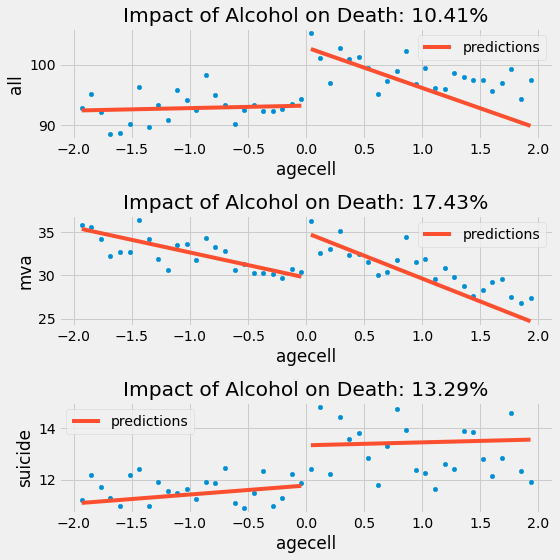
\includegraphics{notebooks/W07. Linear Regression_files/figure-pdf/cell-18-output-1.png}

}

\end{figure}

This Q-Q plot suggests that our residuals are not normally distributed,
as very few of them are on the red line. This is probably due to the
fact that the \texttt{realhrwage} variable is itself highly skewed.

Log transformations are often recommended for skewed data, such as
monetary measures or certain biological and demographic measures. Log
transforming data usually has the effect of spreading out clumps of data
and bringing together spread-out data. So instead of:

\[Hourly\ Income= \beta_0 + \beta_1 \times Years\ of\ Schooling +\epsilon \]

we get:

\[\log{(Hourly\ Income)}= \beta_0 + \beta_1 \times Years\ of\ Schooling +\epsilon \]

In effect, this means changing our belief that there is a linear
relationship between schooling and income (a constant increase in x
leads to a constant increase in y across the whole range of x).
Qualitatively, this means

\begin{Shaded}
\begin{Highlighting}[]
\NormalTok{reg\_df[}\StringTok{\textquotesingle{}logwage\textquotesingle{}}\NormalTok{]}\OperatorTok{=}\NormalTok{np.log(reg\_df[}\StringTok{\textquotesingle{}realhrwage\textquotesingle{}}\NormalTok{])}
\NormalTok{sns.jointplot(data}\OperatorTok{=}\NormalTok{reg\_df, x}\OperatorTok{=}\StringTok{\textquotesingle{}sch\textquotesingle{}}\NormalTok{, y}\OperatorTok{=}\StringTok{\textquotesingle{}logwage\textquotesingle{}}\NormalTok{, kind}\OperatorTok{=}\StringTok{"reg"}\NormalTok{,  scatter\_kws}\OperatorTok{=}\BuiltInTok{dict}\NormalTok{(alpha}\OperatorTok{=}\FloatTok{0.1}\NormalTok{), line\_kws}\OperatorTok{=}\BuiltInTok{dict}\NormalTok{(color}\OperatorTok{=}\StringTok{\textquotesingle{}red\textquotesingle{}}\NormalTok{), height}\OperatorTok{=}\DecValTok{10}\NormalTok{)}
\end{Highlighting}
\end{Shaded}

\begin{figure}[H]

{\centering \includegraphics{notebooks/W07. Linear Regression_files/figure-pdf/cell-19-output-1.png}

}

\end{figure}

A few things are noticeably different in this plot. First, the histogram
of \texttt{logwage} on the far right is a lot less skewed than the
histogram of \texttt{realhrwage}. Consequently, the regression line
seems to fit the data slightly better across the whole range of the
data.

We can generate the same residual histogram and Q-Q plot as before, but
using a model in which \texttt{logwage} is the dependent variable:

\begin{Shaded}
\begin{Highlighting}[]
\NormalTok{log\_model }\OperatorTok{=}\NormalTok{ ols(}\StringTok{\textquotesingle{}logwage \textasciitilde{}  sch\textquotesingle{}}\NormalTok{, data}\OperatorTok{=}\NormalTok{reg\_df).fit()  }\CommentTok{\# fit a model}
\NormalTok{log\_model\_residuals }\OperatorTok{=}\NormalTok{ log\_model.resid }\CommentTok{\# get the residuals}

\CommentTok{\# make the figure wider}
\NormalTok{plt.rcParams[}\StringTok{"figure.figsize"}\NormalTok{] }\OperatorTok{=}\NormalTok{ [}\DecValTok{20}\NormalTok{, }\DecValTok{10}\NormalTok{]}

\NormalTok{f, axes }\OperatorTok{=}\NormalTok{ plt.subplots(}\DecValTok{1}\NormalTok{, }\DecValTok{2}\NormalTok{)}
\NormalTok{sns.histplot(log\_model\_residuals, kde}\OperatorTok{=}\VariableTok{True}\NormalTok{, ax}\OperatorTok{=}\NormalTok{axes[}\DecValTok{0}\NormalTok{]) }\CommentTok{\# plot the residuals}
\NormalTok{axes[}\DecValTok{0}\NormalTok{].set\_title(}\StringTok{\textquotesingle{}Histogram of Residuals\textquotesingle{}}\NormalTok{) }\CommentTok{\# add a title}

\NormalTok{sm.qqplot(log\_model\_residuals, line}\OperatorTok{=}\StringTok{\textquotesingle{}45\textquotesingle{}}\NormalTok{, fit}\OperatorTok{=}\VariableTok{True}\NormalTok{,  ax}\OperatorTok{=}\NormalTok{axes[}\DecValTok{1}\NormalTok{]) }\CommentTok{\# plot the residuals}
\NormalTok{axes[}\DecValTok{1}\NormalTok{].set\_title(}\StringTok{\textquotesingle{}Q{-}Q Plot\textquotesingle{}}\NormalTok{) }\CommentTok{\# add a title}

\NormalTok{plt.show() }\CommentTok{\# show the plot}
\end{Highlighting}
\end{Shaded}

\begin{figure}[H]

{\centering 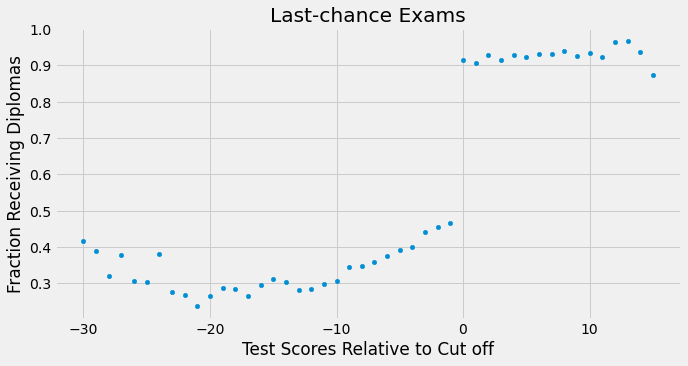
\includegraphics{notebooks/W07. Linear Regression_files/figure-pdf/cell-20-output-1.png}

}

\end{figure}

It's not perfect, but it's a lot better than the unlogged version; a
large proportion of the residuals fall on the red line in the Q-Q plot,
though they diverge at the tips. The histogram of residuals also seems
to be less skewed, and more evenly distributed around 0.

\hypertarget{coefficient-interpretation.}{%
\section{Coefficient
interpretation.}\label{coefficient-interpretation.}}

Only the dependent/response variable is log-transformed. Exponentiate
the coefficient, subtract one from this number, and multiply by 100.
This gives the percent increase (or decrease) in the response for every
one-unit increase in the independent variable. Here's a
\href{https://data.library.virginia.edu/interpreting-log-transformations-in-a-linear-model/\#:~:text=Interpret\%20the\%20coefficient\%20as\%20the,variable\%20increases\%20by\%20about\%200.20\%25.}{full
guide} to interpreting the coefficients on log-transformed variables.

First, let's compare the unlogged and logged models:

\begin{Shaded}
\begin{Highlighting}[]
\NormalTok{table}\OperatorTok{=}\NormalTok{summary\_col( }\CommentTok{\# create a regression table }
\NormalTok{    [model,log\_model], }\CommentTok{\# pass the models to the summary\_col function}
\NormalTok{    stars}\OperatorTok{=}\VariableTok{True}\NormalTok{, }\CommentTok{\# add stars denoting the p{-}values of the coefficient to the table; * p\textless{}0.05, ** p\textless{}0.01, *** p\textless{}0.001}
\NormalTok{    float\_format}\OperatorTok{=}\StringTok{\textquotesingle{}}\SpecialCharTok{\%0.3f}\StringTok{\textquotesingle{}}\NormalTok{, }\CommentTok{\# set the decimal places to 3}
\NormalTok{    model\_names}\OperatorTok{=}\NormalTok{[}\StringTok{\textquotesingle{}Unlogged\textquotesingle{}}\NormalTok{,}\StringTok{\textquotesingle{}Logged\textquotesingle{}}\NormalTok{], }\CommentTok{\# set the name of the model}
\NormalTok{    info\_dict }\OperatorTok{=}\NormalTok{ \{}\StringTok{"N"}\NormalTok{:}\KeywordTok{lambda}\NormalTok{ x: }\StringTok{"}\SpecialCharTok{\{0:d\}}\StringTok{"}\NormalTok{.}\BuiltInTok{format}\NormalTok{(}\BuiltInTok{int}\NormalTok{(x.nobs))\}) }\CommentTok{\# add the number of observations to the table}

\BuiltInTok{print}\NormalTok{(table)}
\end{Highlighting}
\end{Shaded}

\begin{verbatim}

=================================
                Unlogged  Logged 
---------------------------------
Intercept      -6.625*** 1.573***
               (0.266)   (0.012) 
sch            2.033***  0.096***
               (0.019)   (0.001) 
R-squared      0.181     0.191   
R-squared Adj. 0.181     0.191   
N              52750     52750   
=================================
Standard errors in parentheses.
* p<.1, ** p<.05, ***p<.01
\end{verbatim}

Interestingly, we can see that we've also got a 1\% increase in \(R^2\)
just from logging the dependent variable. While the coefficient for
schooling can be interpreted normally for the unlogged model (every
additional year of schooling leads to a \$2.03 increase in hourly
wages), this is not the case for the logged model. We can interpret the
coefficeint in the logged model as follows:

\begin{Shaded}
\begin{Highlighting}[]
\NormalTok{b1}\OperatorTok{=}\NormalTok{log\_model.params.sch }\CommentTok{\# get the coefficient for sch}
\NormalTok{exp\_b1}\OperatorTok{=}\NormalTok{np.exp(b1) }\CommentTok{\# exponentiate the coefficient}

\NormalTok{pct\_change}\OperatorTok{=}\NormalTok{(exp\_b1}\OperatorTok{{-}}\DecValTok{1}\NormalTok{)}\OperatorTok{*}\DecValTok{100} \CommentTok{\# multiply by 100 to get the percentage change}
\BuiltInTok{print}\NormalTok{(}\StringTok{\textquotesingle{}For every additional year of schooling, log wages increase by }\SpecialCharTok{\{\}}\StringTok{\%\textquotesingle{}}\NormalTok{.}\BuiltInTok{format}\NormalTok{(}\BuiltInTok{round}\NormalTok{(pct\_change,}\DecValTok{2}\NormalTok{)))}
\end{Highlighting}
\end{Shaded}

\begin{verbatim}
For every additional year of schooling, log wages increase by 10.04%
\end{verbatim}

\bookmarksetup{startatroot}

\hypertarget{assessed-question-1}{%
\chapter{Assessed Question}\label{assessed-question-1}}

Filter the dataframe to only contain people who work in construction,
extraction and installation. Compared to those who are covered by a
union but not themselves members, what is the difference in log hourly
earnings for union members? Is this difference statistically
significant?

\bookmarksetup{startatroot}

\hypertarget{difference-in-differences}{%
\chapter{Difference in Differences}\label{difference-in-differences}}

\hypertarget{workshop-08-open-in-colab}{%
\section[\emph{Workshop 08} ]{\texorpdfstring{\emph{Workshop 08}
\href{https://colab.research.google.com/github/oballinger/QM2/blob/main/notebooks/W08.\%20Diff-in-Diff.ipynb}{\protect
\includegraphics{index_files/mediabag/colab-badge.png}}}{Workshop 08 Open In Colab}}\label{workshop-08-open-in-colab}}

\hypertarget{aims-6}{%
\subsection{Aims:}\label{aims-6}}

This workshop builds on last week's material, replicating analysis in
published academic research on the relationship between minimum wages
and unemployment.

As always we'll start by importing the libraries I need

\begin{Shaded}
\begin{Highlighting}[]
\CommentTok{\#!pip install linearmodels}
\ImportTok{import}\NormalTok{ pandas }\ImportTok{as}\NormalTok{ pd}
\ImportTok{import}\NormalTok{ seaborn }\ImportTok{as}\NormalTok{ sns}
\ImportTok{import}\NormalTok{ numpy }\ImportTok{as}\NormalTok{ np}
\ImportTok{import}\NormalTok{ plotly}
\ImportTok{import}\NormalTok{ plotly.express }\ImportTok{as}\NormalTok{ px}
\ImportTok{import}\NormalTok{ warnings}
\ImportTok{from}\NormalTok{ statsmodels.formula.api }\ImportTok{import}\NormalTok{ ols}
\ImportTok{from}\NormalTok{ statsmodels.iolib.summary2 }\ImportTok{import}\NormalTok{ summary\_col}
\ImportTok{import}\NormalTok{ matplotlib.pyplot }\ImportTok{as}\NormalTok{ plt}

\NormalTok{warnings.filterwarnings(}\StringTok{\textquotesingle{}ignore\textquotesingle{}}\NormalTok{)}
\NormalTok{sns.}\BuiltInTok{set}\NormalTok{(font\_scale}\OperatorTok{=}\FloatTok{1.5}\NormalTok{)}
\NormalTok{sns.set\_style(}\StringTok{"white"}\NormalTok{)}
\NormalTok{plt.rcParams[}\StringTok{\textquotesingle{}figure.figsize\textquotesingle{}}\NormalTok{] }\OperatorTok{=}\NormalTok{ (}\DecValTok{12}\NormalTok{, }\DecValTok{8}\NormalTok{)}
\end{Highlighting}
\end{Shaded}

\begin{longtable}[]{@{}
  >{\raggedright\arraybackslash}p{(\columnwidth - 0\tabcolsep) * \real{0.3889}}@{}}
\toprule\noalign{}
\begin{minipage}[b]{\linewidth}\raggedright
\#\# Panel Regression
\end{minipage} \\
\midrule\noalign{}
\endhead
\bottomrule\noalign{}
\endlastfoot
\#\# 2. Difference in Differences \\
One of the reasons that we observe a signficant relationship between
unemployment and voting behaviour in last week's workshop is that the
Republican and Democratic parties have opposing views on what to do
about unemployment. Democratic lawmakers have historically been in
favour of increasing the minimum wage to benefit low-income workers,
while Republicans have generally opposed this on the basis that it would
hurt these very workers by increase unemployment. Indeed, classical
economic theory holds that an increase in wages would lead to a
reduction in employment; A business that makes \$100k in revenue per
year and spends all of it on employing 20 people can't suddenly start
paying their workers double their salaries-- unless it fires half of its
workers. This is obviously a simplified model though-- minimum wage laws
typically don't double wages, and businesses don't operate at-cost, they
turn a profit which they could use to pay their workers more. In the
rest of this workshop, we're going to be investigating this question
empirically: \\
\#\#\# Do minimum wage laws increase unemployment? \\
Note that this is a \emph{causal} question; i'm not asking if they're
correlated-- i'm asking if one causes the other. The burden of proof
here is much higher than observing correlations, and we have to think
seriously about \textbf{endogeneity}. In partiuclar, we need to account
for the influence of omitted variables (e.g.~a recession, or the
economic composition of a state), the potential for reverse causality
(states implementing minimum wage laws in response to unemployment
crises), and selection bias. \\
In a lab, you can conduct causal inference by running an experiment. You
can randomly select individuals, split them into a control group and a
treatment group, measure their values in an outcome variable prior to a
treatment, administer a treatment, and measure their respective values
after the treatment. If you observe a change in the outcome variable in
the treatment group after having administered the treatment, you can
interpert that as the causal effect of treatment. This is because we're
able to make a plausible argument that the \textbf{control group can act
as a counterfactual (a stand-in) for the treatment group in the absence
of treatment}. Both groups had the same values before the treatment,
then the only thing that changed between them was the treatment, so if
we observe a change in the outcome variable, it must be due to
treatment. \\
In the real world, we rarely get to run expermients of this kind.
Instead, we have to hunt for \textbf{natural experiments}: situations in
which there is a \textbf{treatment} which we're interested in measuring
the effect of, and two groups that can plausibly act as a treatment and
control group. \\
\textgreater{}
\textbf{\href{https://www.publichealth.columbia.edu/research/population-health-methods/difference-difference-estimation\#:~:text=DID\%20relies\%20on\%20a\%20less,individual\%20level\%20is\%20not\%20possible.}{Difference
in Difference}} is a quasi-experimental design that makes use of
longitudinal data from treatment and control groups to obtain an
appropriate counterfactual to estimate a causal effect. DID is typically
used to estimate the effect of a specific intervention or treatment
(such as a passage of law, enactment of policy, or large-scale program
implementation) by comparing the changes in outcomes over time between a
population that is enrolled in a program (the intervention group) and a
population that is not (the control group). \\
The Difference in Difference model can be estimated as a simple
regression model of the following form: \\
\(\huge Y_{it} = \beta_0 + \beta_1 Treatment_i + \beta_2 Post_t + \beta_3 (Treatment_i \times Post_t) + \varepsilon_{it}\) \\
- \(Treatment_i\) is 0 for the control group and 1 for the treatment
group - \(Post_t\) is 0 for before and 1 for after \\
we can insert the values of \(Treatment\) and \(Post\) using the table
below and see that coefficient (\(\beta_3\)) of the interaction of
\(Treatment\) and \(Post\) is the Difference in Differences (DID)
estimator: \\
\href{https://davidcard.berkeley.edu/papers/njmin-aer.pdf}{Card and
Krueger (1994)} found one such natural experiment, allowing them to
estimate the causal effect of an increase in the state minimum wage on
unemployment using a DiD model; In 1992, New Jersey raised the state
minimum wage from \$4.25 to \$5.05 while the minimum wage in
neighbouring Pennsylvania stayed the same at \$4.25. \\
* Treatmeng Group: New Jersey * Control Group: Pennsylvania *
Pre-Treatment Period: before 1992 * Post-Treatment Period: after 1992 \\
They conducted a survey of 384 fast-food restaurants across both states,
right before and right after the law came into effect in New Jersey,
asking them how many people they employed. They ran a
Difference-in-Differences model, and found that the coefficient
\(\beta_3\) was positive but not statistically significant. In other
words, the average total employees per restaurant \emph{increased} after
the minimum wage increased, but this could have been due to random
chance. \\
That was a long time ago. Things have changed since then, including the
fact that we have access to a lot more data and computational power.
Let's see if we can replicate Card and Krueger's results with more
recent data. I've downloaded data on unemployment, minimum wage levels,
and Gross Domestic Product at the state level going back to 1976. Let's
have a look at minimum wages in New Jersey and Pennsylvania over
time: \\
::: \{.cell\} ``` \{.python .cell-code\}
df\_s=pd.read\_csv(`https://storage.googleapis.com/qm2/wk10/state\_data.csv',
parse\_dates={[}`date'{]}) \# read in the state-level data
did=df\_s{[}df\_s{[}`state'{]}.isin({[}`pennsylvania', `new
jersey'{]}){]} \# subset the data to only include pennsylvania and new
jersey \\
px.line(did, x=`date', y=`minwage', color=`state', title=``Minimum Wages
in New Jersey and Pennsylvania'') \# plot the minimum wage over time ```
::: \\
The plot above sort of looks like a set of descending staircases; this
is for two reasons. The plateaus exist because each row in the dataframe
\texttt{df\_s} is the value of a state in a given \emph{month}, but we
only have minimum wage data for every \emph{year}. So we get 12
consecutive values of minimum wage every year. The reason that the
staircases are descending is because these minimum wages are adjusted
for inflation. No matter where you're from, you've probably heard a
grandparent say something along the lines of ``My parents would send me
to the shops with 25 cents to buy groceries for the week'', but now it
costs £9 for a bag of chips. That's inflation-- every year things tend
to get slightly more expensive, so if the same \emph{absolute} minimum
wage actually diminishes in ``real'' terms, which is what the variable
\texttt{minwage} measures. Incidentally, this is one of the main reasons
University staff have been on
\href{https://www.ucu.org.uk/article/11830/University-staff-pay-cut-by-20-new-figures-show}{strike}.
Anyway. Back to minimum wages. \\
This plot shows that for the past fifty years, New Jersey and
Pennsylvania have had largely similar minimum wage policies. There have
been a couple moments of divergence, including in the 1990s when the
Card and Krueger study was conducted. However, the biggest divergence
actually started taking place in 2014 when New Jersey seems to have
begun taking a wildly different approach. While Pennsylvania has had the
same minimum wage since 2008 (and therefore seen a decline in
inflation-adjusted wages), New Jersey has raised the minimum wage
significantly twice. In 2020, New Jersey's minimum wage was around 50\%
higher than Pennsylvania's. We can exploit the fact that these two
states have historically had similar minimum wage laws but have recently
experienced a big divergence to see if that change in minimum wages has
resulted in a change in employment levels. \\
Our Difference-in-Differences setup is as follows: \\
\(\large Unemployment_{state, year} = \beta_0 + \beta_1 Treatment_{state} + \beta_2 Post_{year} + \beta_3 (Treatment_{state} \times Post_{year}) + \beta_4 GDP_{state,year} + \varepsilon_{it}\) \\
* New Jersey is the \textbf{treatment group} * Pennsylvania is the
\textbf{control group} * Years before 2014 is the \textbf{pre-treatment
period} * Years after 2014 is the \textbf{post-treatment period} \\
::: \{.cell\} \\
Before we proceed with the analysis, though, we need to satisfy two
assumptions that will allow us to argue that Pennsylvania can act as a
valid control group for New Jersey: \\
1. No simultaneous treatments: * If, for example, New Jersey suddenly
entered a massive recession in 2014 as well, we couldn't really argue
that resulting effects on employment are due solely to the minimum wage
law. To account for this, we'll be including state-level GDP as an
additional independent variable in our DiD model. 2. Parallel Trends: *
Both states have to have been experiencing similar trends in the
\textbf{dependent variable} (unemployment) prior to the treatment
(minimum wage law). If they were trending in opposite directions for
unobserved reasons, ensuing differences in unemployment may be due to
those unobserved reasons rather than the treatment. * We can check this
by plotting the dependent variable for both groups over time, and
indicating the timing of the treatment. \\
::: \{.cell\} \\
This plot shows a big spike in unemployment occurring for both
Pennsylvania and New Jersey as a result of the 2008 financial crisis.
New jersey had a higher unemployment rate than Pennsylvania, but their
trends are largely parallel and decreasing after 2012. In the years
following the minimum wage law, New Jersey's unemployment rate actually
dips below Pennsylvania's for the first time in years. Let's look at
this in the form of boxplots: \\
::: \{.cell\} \\
This plot is fascinating in and of itself. The two box plots on the left
show the unemployment values of the counties prior to the minimum wage
law in 2014, while the two on the right show their values after the
minimum wage increases. Pennsylvania (the ``control'' group) is colored
in blue, and New Jersey (the ``treatment'' group) is colored orange.
Prior to the minimum wage increase in 2014, Pennsylvania (blue) has a
lower unemployment rate than New Jersey (orange). In the years following
New Jersey's passage of the minimum wage law, New Jersey actually has a
\emph{lower} unemployment rate than Pennsylvania! This is the only
boxplot where the ``treatment'' (a minimum wage law) is being applied,
and it has the lowest unemployment rate. \\
Let's see if this difference is statistically signfiicant, and calculate
a treatment effect: \\
::: \{.cell\} \\
There are some really interesting results from this model-- let's
interpret the coefficients one by one. \\
* \texttt{gdp}: GDP is inversely related to unemployment. This makes
sense: GDP basically measures the total amount of economic activity, so
more economic activity = more employment. * \texttt{post}: this
coefficient is negative, but statistically insignificant at the 0.05
level; it indicates that unemployment \emph{generally} decreased for
both groups, but that this could be due to random chance. *
\texttt{treatment}: again negative but insignficant, meaning that there
is no significant difference in unemployment levels between NJ and PA
over the entire period. * \texttt{post\_treatment}: this is our
difference-in-differences estimator, and reflects the causal effect of
treatment. It is negative and statistically significant. If we believe
that the asusmptions of our model are satisfied, we can claim that: *
\textbf{The introduction of a minimum wage in New Jersey led to a 1.95\%
decrease in unemployment relative to Pennsylvania} \\
This is a bold claim. We should do our best to back it up. Notice that
i've sort of arbitrarily chosen a window of dates around the minimum
wage law-- maybe this result is a fluke, due to the timespan ive
chosen. \\
To address this concern, I'll run the same model 10 times, starting with
a really small time window-- just one year on either side of the law--
and progressively expand it. \\
::: \{.cell\} ``` \{.python .cell-code\} models={[}{]} \# create empty
list to store the models names={[}{]} \# create empty list to store the
names of the models \\
for window in range(1,10): \# loop through years from 2000 to 2020 in
increments of 4
did=df\_s{[}(df\_s{[}`date'{]}\textgreater=str(2014-window)+`-01-01') \&
(df\_s{[}`date'{]}\textless=str(2014+window)+`-01-01') \&
df\_s{[}`state'{]}.isin({[}`pennsylvania', `new jersey'{]}){]} \# subset
the data within the window of interest around 2014
did{[}`post'{]}=np.where(did{[}`date'{]}\textgreater=`2014-01-01',1,0)
\# create a dummy variable indicating the period after the minimum wage
increase did{[}`treatment'{]}=np.where(did{[}`state'{]}==`new
jersey',1,0) \# create a dummy variable for treatment
did{[}`post\_treatment'{]}=did{[}`post'{]}*did{[}`treatment'{]} \#
create an interaction term between the post and treatment variables
did\_model = ols(`unemployment \textasciitilde{} gdp+ post + treatment +
post\_treatment', did).fit() \# run the difference in difference
model \\
models.append(did\_model) \# append the model to the list of models
names.append(`±'+str(window)+' Year') \# append the name of the model to
the list of names \\
table=summary\_col( \# create a regression table models, \# pass the
models to the summary\_col function stars=True, \# add stars denoting
the p-values of the coefficient to the table; * p\textless0.05, **
p\textless0.01, *** p\textless0.001 float\_format=`\%0.3f', \# set the
decimal places to 3 model\_names=names, \# set the names of the model
info\_dict = \{``N'':lambda x: ``\{0:d\}''.format(int(x.nobs))\}) \# add
the number of observations to the table \\
print(table) \# print the table \\
``` ::: \\
The row we're mainly interested in is the \texttt{post\_treatment}
coefficient, the treatment effect. It remains significant and negative
in all time periods smaller than 8 years, after which point it becomes
insignificant; \\
How do you think this affects our conclusion? \\
\# Assessed Question \\
Now we've got evidence that minimum wage laws may actually
\emph{decrease} unemployment in the case of New Jersey and Pennsylvania.
But we've got quite a bit of data, and minimum wages change frequently.
Let's find another example where we may be able to run a difference in
differences regression to see if this trend holds in a different
context. \\
Below, I've picked out Arizona and Louisiana; they had nearly the exact
same minimum wage for seven years, but in 2007 Arizona nearly tripled
its minimum wage while Louisiana kept it the same (\ldots by not having
one). \\
::: \{.cell\} \\
Run a difference in differences regression to measure the effect of this
minimum wage increase on unemployment. Define three variables (post,
treatment, post\_treatment), and include just these three variables in
the model. \\
* Part A: What is the effect of the minimum wage increase on
unemployment in the case of Arizona and Louisiana? * Part B: Difference
in Differences designs have two assumptions: parallel trends, and no
simultaneous treatment. Can you think of any events that ocurred in 2008
that might violate the ``no simultaneous treatment'' assumption? \\
 \\
\texttt{\{=html\}\ \textless{}!-\/-\ quarto-file-metadata:\ eyJyZXNvdXJjZURpciI6Im5vdGVib29rcyIsImJvb2tJdGVtVHlwZSI6ImNoYXB0ZXIiLCJib29rSXRlbU51bWJlciI6MTAsImJvb2tJdGVtRmlsZSI6Ii4vbm90ZWJvb2tzL1cwOS4gUmVncmVzc2lvbiBEaXNjb250aW51aXR5LmlweW5iIiwiYm9va0l0ZW1EZXB0aCI6MH0=\ -\/-\textgreater{}} \\
\# Regression Discontinuity \\
\#\# \emph{Workshop 09}
\href{https://colab.research.google.com/github/oballinger/QM2/blob/main/notebooks/W09.\%20Regression\%20Discontinuity.ipynb}{
\includegraphics{index_files/mediabag/colab-badge.png}} \\
In this final week, we're going to look at Regression Discontinuity
Designs (RDD). We'll look into discontinuities in two types of
variables: \\
1. Spatial discontinuities 2. Temporal discontinuities \\
::: \{.cell\} \\
::: \{.cell-output .cell-output-stdout\} \\
::: \{.cell tags=`{[}``hide-input''{]}' execution\_count=2\} ```
\{.python .cell-code\} import warnings
warnings.filterwarnings(`ignore') \\
import pandas as pd import numpy as np from matplotlib import style from
matplotlib import pyplot as plt import seaborn as sns import
statsmodels.formula.api as smf import geopandas as gpd from
statsmodels.formula.api import ols \\
\%matplotlib inline \\
style.use(``fivethirtyeight'') ``` ::: \\
\# Spatial Discontinuities \\
Last week, we set up a difference model and made causal claims about the
effect of minimum wage laws on unemployment. We did this by treating
Pennsylvania as a control group for New Jersey on the basis that they
had similar trends in unemployment before the minimum wage law, and
diverging trends after, and no other shock coincided with this
policy. \\
We could still poke some holes in that-- NJ seems to have fared worse
than PA after the 2008 crisis; maybe more people work in finance in NJ.
Indeed, Jersey City is across the water from Manhattan, America's
financial centre. Bankers would be hard hit by a financial crisis, but
are probably not that affected by minimum wage laws. Conversely,
Pennsylvania is the 3rd largest coal-producing state in the U.S.-- coal
miners are probably less affected by financial crises, but more likely
to be earning minimum wage. As such, increasing the minimum wage in a
place where most people are bankers probably has less of an effect on
unemployment compared to an area where everyone is a coal miner. \\
Running a state-level analysis is subject to this sort of selection
bias, since by looking at state averages we're effectively comparing
places like Jersey City to places like
\href{https://en.wikipedia.org/wiki/Centralia,_Pennsylvania}{Centralia},
a coal-mining town in central Pennsylvania which saw its population
decline from 1000 in 1980 to just five residents in 2020. So the next
step in our analysis might be to try to compare apples to apples. There
are a number of ways of doing this-- we could look at the unemployment
rate by industry, for example. But what if we didn't want to rely on
pre-trends, or if we didn't even have data prior to the treatment? This
is often the case \\
To build a more valid counterfactual, we can drill even deeper to find
even more similar comparison groups using a \textbf{Regression
Discontinuity Design (RDD)} using county (rather than state) level
data. \\
\textgreater{}
\textbf{\href{https://www.princeton.edu/~davidlee/wp/RDDEconomics.pdf}{Regression
Discontinuity Designs}} are a method of estimating treatment effects in
a nonexperimental setting where treatment is determined by whether an
observed ``assignment'' variable exceeds a known cutoff point. If the
cutoff is exogenous to the treatment, observations in the vicinity of
this cutoff are likely to be very similar, and assignment to the
treatment or control group can be considered as good as random. \\
RDD models generally take the following form: \\
\(\huge Y_{i} = \beta_0 + \beta_1 R_i + \beta_2 T_i + \varepsilon_{i}\) \\
\(\large T_i=    \begin{cases}
1 & R_i>c\\
0 & R_i<c\\
\end{cases} \) \\
Where R is the ``running variable'', T is the treatment variable, and c
is a cutoff in the running variable assigning observations to the
``treatment'' or ``control'' groups. \\
In our case, the treatment is the minimum wage law passed in NJ in 2014.
We want to be looking at the period after this to pick up on any changes
in employment. The \textbf{assignment variable} in this case could be
the distance of a county to the border between the two states, and the
sharp cutoff would be the border itself. Counties on the border counties
are probably much more similar to each other than other, farther away
counties: this would exclude both Jersey City (in the far east of NJ)
and Centralia (in the centre of PA). \\
Indeed, several cities are divided by the border between these states
including Philladelphia, the capital city of Pennsylvania: \\
::: \{.cell execution\_count=3\} \\
::: \{.cell-output .cell-output-display\} \\
On the left side of the river is Philladelphia, PA, while on the right
side is Camden, NJ. The code below uses the county shapefile we used
before to isolate the counties in NJ and PA that are on the border. \\
::: \{.cell\} ``` \{.python .cell-code\}
counties=pd.read\_csv(`https://storage.googleapis.com/qm2/wk10/county\_labor.csv',
dtype=\{`county\_fips':str\}) \# read in the county labor data shp =
gpd.read\_file(`data/geojson-counties-fips.json') \# read in the
counties shapefile \\
subset=shp{[}shp{[}`STATE'{]}.isin({[}`34',`42'{]}){]} \# new jersey =
34, pennsylvania = 42, new york = 36 \\
subset{[}`neighbors'{]}= 0 \# create a new column called neighbors \\
for index, row in subset.iterrows(): \# iterate through each row in the
counties shapefile buffered= row{[}`geometry'{]}.buffer(0.1) \# create a
buffer around the county so that it overlaps with its neighbors
neighbors =
list(set(subset{[}subset.geometry.overlaps(buffered){]}.STATE.tolist()).difference({[}row.STATE{]}))
\# check which counties overlap with the buffer, grab the state code,
and remove the current county's state code subset.at{[}index,
``neighbors''{]} = ``,''.join(neighbors) \# add the list of neighbors to
the neighbors column \\
subset{[}`border'{]}=np.where(subset{[}`neighbors'{]}=='\,',0,1) \#
create a new column called border that is 1 if the county is on the
border and 0 if it is not \\
subset{[}`viscol'{]}=subset{[}`STATE'{]}.astype(int)+subset{[}`border'{]}
\# create a new column that combines the state code and the border
column subset.plot(column=`viscol',legend=False, figsize=(20,10),
cmap=`RdYlGn') \# plot the counties and color them by the border column
plt.title(`Border Counties in New Jersey and Pennsylvania', fontsize=20)
\# add a title ``` \\
::: \{.cell-output .cell-output-display execution\_count=23\} \\
::: \{.cell-output .cell-output-display\}
\includegraphics{notebooks/W09. Regression Discontinuity_files/figure-pdf/cell-5-output-2.png}
::: ::: \\
We can now restrict our sample to only include counties within a set
distance the border, and set up a regression discontinuity design in
which: \\
* unemployment is the dependent variable. * state (NJ/PA) is the
treatment variable. * distance from the border is the running
variable. \\
::: \{.cell execution\_count=27\} ``` \{.python .cell-code\}
border\_counties=subset{[}subset{[}`border'{]}==1{]}{[}`id'{]}.tolist()
\# create a list of the border counties
rdd=counties{[}(counties{[}`year'{]}\textgreater2007)\&(counties{[}`county\_fips'{]}.isin(border\_counties)){]}
\# subset the counties data to only include border counties and years
after 2007 rdd\_model = ols(`unemployment \textasciitilde{} C(state)',
rdd{[}rdd{[}`year'{]}\textgreater2014{]}).fit() \\
print(rdd\_model.summary()) ``` \\
::: \{.cell-output .cell-output-stdout\} ``` OLS Regression Results
==============================================================================
Dep. Variable: unemployment R-squared: 0.032 Model: OLS Adj. R-squared:
0.023 Method: Least Squares F-statistic: 3.394 Date: Fri, 01 Dec 2023
Prob (F-statistic): 0.0683 Time: 12:53:28 Log-Likelihood: -211.58
No.~Observations: 105 AIC: 427.2 Df Residuals: 103 BIC: 432.5 Df Model:
1 Covariance Type: nonrobust
==================================================================================
coef std err t P\textgreater\textbar t\textbar{} {[}0.025 0.975{]} \\
\end{longtable}

Intercept 5.2518 0.245 21.446 0.000 4.766 5.737 C(state){[}T.42{]}
0.6605 0.358 1.842 0.068 -0.051 1.371
==============================================================================
Omnibus: 21.953 Durbin-Watson: 0.637 Prob(Omnibus): 0.000 Jarque-Bera
(JB): 27.712 Skew: 1.141 Prob(JB): 9.60e-07 Kurtosis: 4.061 Cond.
No.~2.55
==============================================================================

Notes: \href{http://www.literateprogramming.com/lpquotes.html}{1}
Standard Errors assume that the covariance matrix of the errors is
correctly specified.

\begin{verbatim}
:::
:::



This gives us a much better idea of the impact of the minimum wage law by discarding counties that are very far away from eachother and thus dissimilar. We can see that border counties in Pennsylvania saw a 0.66% *increase* in unemployment relative to border counties in New Jersey, in the years following the latter's implementation of the minimum wage increase. This difference, however, is not statistically significant. 

This example captures the basic intuition behind regression discontinuity, but we might worry that the minimum wage law isn't the only thing that changes as the discontinutiy (i.e., isn't the only thing that changes between NJ and PA). 

It is quite common to use distance as a running variable in RDD, and if you're interested in a review of the literature on spatial RDD models check out [this article](https://www.jstor.org/stable/24572845). 

To get a firm grasp of the intuition and mechanics behind RDD, we'll use a more straightforward example. 

## Is Alcohol Killing You?

A very relevant public policy question is what should be the minimal drinking age. Most countries, Brazil included, set it to be 18 year, but in the US (most states) it is currently 21. So, is it the case that the US is being overly prudent and that they should lower their minimal drinking age? Or is it the case that other countries should make their legal drinking age higher? 

One way to look at this question is from a [mortality rate perspective (Carpenter and Dobkin, 2009)](https://www.aeaweb.org/articles?id=10.1257/app.1.1.164). From the public policy standpoint, one could argue that we should lower the mortality rate as much as possible. If alcohol consumption increases the mortality rate by a lot, we should avoid lowering the minimum drinking age. This would be consistent with the objective of lowering deaths caused by alcohol consumption.

To estimate the impacts of alcohol on death, we could use the fact that legal drinking age imposes a discontinuity on nature. In the US, those just under 21 years don't drink (or drink much less) while those just older than 21 do drink. This means that the probability of drinking jumps at 21 years and that is something we can explore with an RDD.

To do so we can grab some mortality data aggregated by age. Each row is the average age of a group of people and the average mortality by all causes (`all`), by moving vehicle accident (`mva`) and by suicide (`suicide`). 

::: {.cell}
``` {.python .cell-code}
drinking = pd.read_csv("https://storage.googleapis.com/qm2/rdd/drinking.csv")
drinking.head()[["agecell", "all", "mva", "suicide"]]
\end{verbatim}

\begin{longtable}[]{@{}lllll@{}}
\toprule\noalign{}
& agecell & all & mva & suicide \\
\midrule\noalign{}
\endhead
\bottomrule\noalign{}
\endlastfoot
0 & 19.068493 & 92.825400 & 35.829327 & 11.203714 \\
1 & 19.150684 & 95.100740 & 35.639256 & 12.193368 \\
2 & 19.232876 & 92.144295 & 34.205650 & 11.715812 \\
3 & 19.315070 & 88.427760 & 32.278957 & 11.275010 \\
4 & 19.397260 & 88.704940 & 32.650967 & 10.984314 \\
\end{longtable}

:::

Just to aid visibility (and for another important reason we will see
later) we will centralize the running variable \texttt{agecell} at the
threshold 21.

\begin{Shaded}
\begin{Highlighting}[]
\NormalTok{drinking[}\StringTok{"agecell"}\NormalTok{] }\OperatorTok{{-}=} \DecValTok{21}
\end{Highlighting}
\end{Shaded}

If we plot the multiple outcome variables (\texttt{all}, \texttt{mva},
\texttt{suicide}) with the runing variable on the x axis, we get some
visual cue about some sort of jump in mortality as we cross the legal
drinking age.

\begin{Shaded}
\begin{Highlighting}[]
\NormalTok{plt.figure(figsize}\OperatorTok{=}\NormalTok{(}\DecValTok{8}\NormalTok{,}\DecValTok{8}\NormalTok{))}
\NormalTok{ax }\OperatorTok{=}\NormalTok{ plt.subplot(}\DecValTok{3}\NormalTok{,}\DecValTok{1}\NormalTok{,}\DecValTok{1}\NormalTok{)}
\NormalTok{drinking.plot.scatter(x}\OperatorTok{=}\StringTok{"agecell"}\NormalTok{, y}\OperatorTok{=}\StringTok{"all"}\NormalTok{, ax}\OperatorTok{=}\NormalTok{ax)}
\NormalTok{plt.title(}\StringTok{"Death Cause by Age (Centered at 0)"}\NormalTok{)}

\NormalTok{ax }\OperatorTok{=}\NormalTok{ plt.subplot(}\DecValTok{3}\NormalTok{,}\DecValTok{1}\NormalTok{,}\DecValTok{2}\NormalTok{, sharex}\OperatorTok{=}\NormalTok{ax)}
\NormalTok{drinking.plot.scatter(x}\OperatorTok{=}\StringTok{"agecell"}\NormalTok{, y}\OperatorTok{=}\StringTok{"mva"}\NormalTok{, ax}\OperatorTok{=}\NormalTok{ax)}

\NormalTok{ax }\OperatorTok{=}\NormalTok{ plt.subplot(}\DecValTok{3}\NormalTok{,}\DecValTok{1}\NormalTok{,}\DecValTok{3}\NormalTok{, sharex}\OperatorTok{=}\NormalTok{ax)}
\NormalTok{drinking.plot.scatter(x}\OperatorTok{=}\StringTok{"agecell"}\NormalTok{, y}\OperatorTok{=}\StringTok{"suicide"}\NormalTok{, ax}\OperatorTok{=}\NormalTok{ax)}\OperatorTok{;}
\end{Highlighting}
\end{Shaded}

\begin{figure}[H]

{\centering 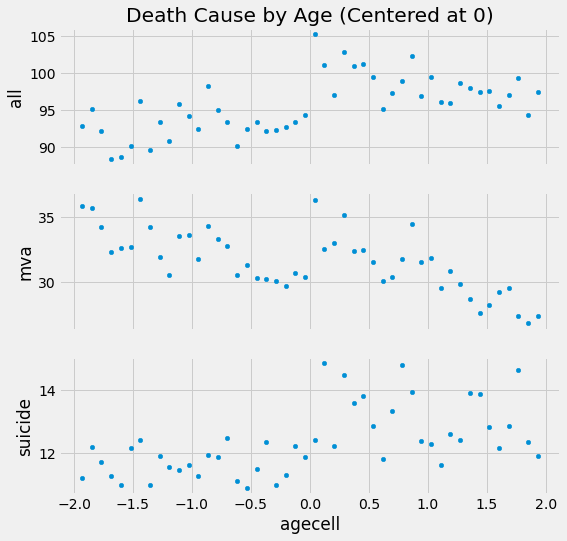
\includegraphics{notebooks/W09. Regression Discontinuity_files/figure-pdf/cell-9-output-1.png}

}

\end{figure}

There are some cues, but we need more than that. What exactly is the
effect of drinking on mortality at the threshold? And what is the
standard error on that estimate?

\hypertarget{rdd-estimation}{%
\section{RDD Estimation}\label{rdd-estimation}}

The key assumption that RDD relies on is the smoothness of the potential
outcome at the threshold. We can think of RDD as a local randomized
trial. For those at the threshold, the treatment could have gone either
way and, by chance, some people fell below the threshold, and some
people fell above. In our example, at the same point in time, some
people are just above 21 years and some people are just below 21. What
determines this is if someone was born some days later or not, which is
pretty random. For this reason, RDD provides a very compelling causal
story. It is not the golden standard of RCT, but it is close.

Now, to estimate the treatment effect at the threshold, all we need to
do is estimate both of the limits in the formula above and compare them.
The simplest way to do that is by running a linear regression

To make it work, we interact a dummy for being above the threshold with
the running variable

\$ y\_i = \beta\_0 + \beta\_1 r\_i + \beta\_2
\mathcal{1}\{r\_i\textgreater c\} + \beta\_3
\mathcal{1}\{r\_i\textgreater c\} r\_i \$

Essentially, this is the same as fitting a linear regression above the
threshold and another below it. The parameter \(\beta_0\) is the
intercept of the regression below the threshold and \(\beta_0+\beta_2\)
is the intercept for the regression above the threshold.

Here is where the trick of centering the running variable at the
threshold comes into play. After this pre-processing step, the threshold
becomes zero. This causes the intercept \(\beta_0\) to be the predicted
value at the threshold, for the regression below it. By the same
reasoning, \(\beta_0+\beta_2\) is the limit of the outcome from above.

Here is what this looks like in code for the case where we want to
estimate the effect of alcohol consumption on death by all causes at 21
years.

\begin{Shaded}
\begin{Highlighting}[]
\NormalTok{rdd\_df }\OperatorTok{=}\NormalTok{ drinking.assign(threshold}\OperatorTok{=}\NormalTok{(drinking[}\StringTok{"agecell"}\NormalTok{] }\OperatorTok{\textgreater{}} \DecValTok{0}\NormalTok{).astype(}\BuiltInTok{int}\NormalTok{))}
\NormalTok{model }\OperatorTok{=}\NormalTok{ smf.wls(}\StringTok{"all\textasciitilde{} agecell * threshold "}\NormalTok{, rdd\_df).fit()}
\BuiltInTok{print}\NormalTok{(model.summary())}
\end{Highlighting}
\end{Shaded}

\begin{verbatim}
                            WLS Regression Results                            
==============================================================================
Dep. Variable:                    all   R-squared:                       0.668
Model:                            WLS   Adj. R-squared:                  0.645
Method:                 Least Squares   F-statistic:                     29.47
Date:                Fri, 10 Mar 2023   Prob (F-statistic):           1.33e-10
Time:                        11:18:58   Log-Likelihood:                -105.64
No. Observations:                  48   AIC:                             219.3
Df Residuals:                      44   BIC:                             226.8
Df Model:                           3                                         
Covariance Type:            nonrobust                                         
=====================================================================================
                        coef    std err          t      P>|t|      [0.025      0.975]
-------------------------------------------------------------------------------------
Intercept            93.6184      0.932    100.399      0.000      91.739      95.498
agecell               0.8270      0.819      1.010      0.318      -0.823       2.477
threshold             7.6627      1.319      5.811      0.000       5.005      10.320
agecell:threshold    -3.6034      1.158     -3.111      0.003      -5.937      -1.269
==============================================================================
Omnibus:                        0.294   Durbin-Watson:                   1.965
Prob(Omnibus):                  0.863   Jarque-Bera (JB):                0.411
Skew:                           0.167   Prob(JB):                        0.814
Kurtosis:                       2.693   Cond. No.                         7.75
==============================================================================

Notes:
[1] Standard Errors assume that the covariance matrix of the errors is correctly specified.
\end{verbatim}

This model is telling us that mortality increases by 7.6627 points with
the consumption of alcohol. Another way of putting this is that alcohol
increases the chance of death by all causes by 8\%
\((100*((7.6627+93.6184)/93.6184 - 1))\). Notice that this also gives us
standard errors for our causal effect estimate. In this case, the effect
is statistically significant, since the p-value is below 0.01. We can
calculate the treatment effect programattically as follows:

\begin{Shaded}
\begin{Highlighting}[]
\NormalTok{ate\_pct }\OperatorTok{=} \DecValTok{100}\OperatorTok{*}\NormalTok{((model.params[}\StringTok{"threshold"}\NormalTok{] }\OperatorTok{+}\NormalTok{ model.params[}\StringTok{"Intercept"}\NormalTok{])}\OperatorTok{/}\NormalTok{model.params[}\StringTok{"Intercept"}\NormalTok{] }\OperatorTok{{-}} \DecValTok{1}\NormalTok{)}

\BuiltInTok{print}\NormalTok{(}\StringTok{"Alcohol increases the chance of death by all causes by }\SpecialCharTok{\{\}}\StringTok{\%"}\NormalTok{.}\BuiltInTok{format}\NormalTok{(np.}\BuiltInTok{round}\NormalTok{(ate\_pct,}\DecValTok{2}\NormalTok{)))}
\end{Highlighting}
\end{Shaded}

\begin{verbatim}
Alcohol increases the chance of death by all causes by 8.19%
\end{verbatim}

If we want to verify this model visually, we can show the predicted
values on the data that we have. You can see that it is as though we had
2 regression models: one for those above the threshold and one for below
it.

\begin{Shaded}
\begin{Highlighting}[]
\NormalTok{ax }\OperatorTok{=}\NormalTok{ drinking.plot.scatter(x}\OperatorTok{=}\StringTok{"agecell"}\NormalTok{, y}\OperatorTok{=}\StringTok{"all"}\NormalTok{, color}\OperatorTok{=}\StringTok{"C0"}\NormalTok{)}
\NormalTok{drinking.assign(predictions}\OperatorTok{=}\NormalTok{model.fittedvalues).plot(x}\OperatorTok{=}\StringTok{"agecell"}\NormalTok{, y}\OperatorTok{=}\StringTok{"predictions"}\NormalTok{, ax}\OperatorTok{=}\NormalTok{ax, color}\OperatorTok{=}\StringTok{"C1"}\NormalTok{)}
\NormalTok{plt.title(}\SpecialStringTok{f"Impact of Alcohol on Death: }\SpecialCharTok{\{}\NormalTok{np}\SpecialCharTok{.}\BuiltInTok{round}\NormalTok{(ate\_pct, }\DecValTok{2}\NormalTok{)}\SpecialCharTok{\}}\SpecialStringTok{\% }\CharTok{\textbackslash{}n}\SpecialStringTok{ p=}\SpecialCharTok{\{}\NormalTok{np}\SpecialCharTok{.}\BuiltInTok{round}\NormalTok{(model.pvalues[}\StringTok{\textquotesingle{}threshold\textquotesingle{}}\NormalTok{], }\DecValTok{3}\NormalTok{)}\SpecialCharTok{\}}\SpecialStringTok{, R2=}\SpecialCharTok{\{}\NormalTok{np}\SpecialCharTok{.}\BuiltInTok{round}\NormalTok{(model.rsquared, }\DecValTok{3}\NormalTok{)}\SpecialCharTok{\}}\SpecialStringTok{"}\NormalTok{)}
\NormalTok{plt.show()}
\end{Highlighting}
\end{Shaded}

\begin{figure}[H]

{\centering \includegraphics{notebooks/W09. Regression Discontinuity_files/figure-pdf/cell-12-output-1.png}

}

\end{figure}

\bookmarksetup{startatroot}

\hypertarget{assessed-question-2}{%
\chapter{Assessed Question}\label{assessed-question-2}}

You'll remember from the lecture slides that the model we've fit above
is a linear, different slopes design. Try fitting the following models:

\begin{enumerate}
\def\labelenumi{\arabic{enumi}.}
\tightlist
\item
  Linear, Same Slopes
\item
  Linear, Different Slopes
\end{enumerate}

Pay attention to the treatment effect. Is it consistent across models?
Which model has the highest treatment effect? Which model fits the best?

\hypertarget{kernel-weighting}{%
\subsection{Kernel Weighting}\label{kernel-weighting}}

Regression Discontinuity relies heavily on the extrapolations properties
of linear regression. Since we are looking at the values at the
beginning and end of 2 regression lines, we better get those limits
right. What can happen is that regression might focus too much on
fitting the other data points at the cost of a poor fit at the
threshold. If this happens, we might get the wrong measure of the
treatment effect.

One way to solve this is to give higher weights for the points that are
closer to the threshold. There are many ways to do this, but a popular
one is to reweight the samples with the \textbf{triangular kernel}

\$ K(R, c, h) = \mathcal{1}\{\textbar R-c\textbar{} \leq h\} *
\bigg(1-\frac{|R-c|}{h}\bigg) \$

The first part of this kernel is an indicator function to whether we are
close to the threshold. How close? This is determined by a bandwidth
parameter \(h\). The second part of this kernel is a weighting function.
As we move away from the threshold, the weights get smaller and smaller.
These weights are divided by the bandwidth. If the bandwidth is large,
the weights get smaller at a slower rate. If the bandwidth is small, the
weights quickly go to zero.

To make it easier to understand, here is what the weights look like for
this kernel applied to our problem. I've set the bandwidth to be 1 here,
meaning we will only consider data from people that are no older than 22
years and no younger than 20 years.

\begin{Shaded}
\begin{Highlighting}[]
\KeywordTok{def}\NormalTok{ kernel(R, c, h):}
\NormalTok{    indicator }\OperatorTok{=}\NormalTok{ (np.}\BuiltInTok{abs}\NormalTok{(R}\OperatorTok{{-}}\NormalTok{c) }\OperatorTok{\textless{}=}\NormalTok{ h).astype(}\BuiltInTok{float}\NormalTok{)}
    \ControlFlowTok{return}\NormalTok{ indicator }\OperatorTok{*}\NormalTok{ (}\DecValTok{1} \OperatorTok{{-}}\NormalTok{ np.}\BuiltInTok{abs}\NormalTok{(R}\OperatorTok{{-}}\NormalTok{c)}\OperatorTok{/}\NormalTok{h)}
\end{Highlighting}
\end{Shaded}

\begin{Shaded}
\begin{Highlighting}[]
\NormalTok{plt.plot(drinking[}\StringTok{"agecell"}\NormalTok{], kernel(drinking[}\StringTok{"agecell"}\NormalTok{], c}\OperatorTok{=}\DecValTok{0}\NormalTok{, h}\OperatorTok{=}\DecValTok{1}\NormalTok{))}
\NormalTok{plt.xlabel(}\StringTok{"agecell"}\NormalTok{)}
\NormalTok{plt.ylabel(}\StringTok{"Weight"}\NormalTok{)}
\NormalTok{plt.title(}\StringTok{"Kernel Weight by Age"}\NormalTok{)}\OperatorTok{;}
\end{Highlighting}
\end{Shaded}

\begin{figure}[H]

{\centering \includegraphics{notebooks/W09. Regression Discontinuity_files/figure-pdf/cell-15-output-1.png}

}

\end{figure}

If we apply these weights to our original problem, the impact of alcohol
gets bigger, at least for all causes. It jumps from 7.6627 to 9.7004.
The result remains very significant. Also, notice that I'm using
\texttt{wls} instead of \texttt{ols}

\begin{Shaded}
\begin{Highlighting}[]
\NormalTok{model }\OperatorTok{=}\NormalTok{ smf.wls(}\StringTok{"all\textasciitilde{}agecell*threshold"}\NormalTok{, rdd\_df,}
\NormalTok{                weights}\OperatorTok{=}\NormalTok{kernel(drinking[}\StringTok{"agecell"}\NormalTok{], c}\OperatorTok{=}\DecValTok{0}\NormalTok{, h}\OperatorTok{=}\DecValTok{1}\NormalTok{)).fit()}

\NormalTok{model.summary().tables[}\DecValTok{1}\NormalTok{]}
\end{Highlighting}
\end{Shaded}

\begin{longtable}[]{@{}lllllll@{}}
\toprule\noalign{}
\endhead
\bottomrule\noalign{}
\endlastfoot
& coef & std err & t & P\textgreater\textbar t\textbar{} & {[}0.025 &
0.975{]} \\
Intercept & 93.2002 & 0.731 & 127.429 & 0.000 & 91.726 & 94.674 \\
agecell & 0.4109 & 1.789 & 0.230 & 0.819 & -3.196 & 4.017 \\
threshold & 9.7004 & 1.034 & 9.378 & 0.000 & 7.616 & 11.785 \\
agecell:threshold & -7.1759 & 2.531 & -2.835 & 0.007 & -12.276 &
-2.075 \\
\end{longtable}

\begin{Shaded}
\begin{Highlighting}[]
\NormalTok{ax }\OperatorTok{=}\NormalTok{ drinking.plot.scatter(x}\OperatorTok{=}\StringTok{"agecell"}\NormalTok{, y}\OperatorTok{=}\StringTok{"all"}\NormalTok{, color}\OperatorTok{=}\StringTok{"C0"}\NormalTok{)}
\NormalTok{drinking.assign(predictions}\OperatorTok{=}\NormalTok{model.fittedvalues).plot(x}\OperatorTok{=}\StringTok{"agecell"}\NormalTok{, y}\OperatorTok{=}\StringTok{"predictions"}\NormalTok{, ax}\OperatorTok{=}\NormalTok{ax, color}\OperatorTok{=}\StringTok{"C1"}\NormalTok{)}
\NormalTok{plt.title(}\StringTok{"Regression Discontinuity (Local Regression)"}\NormalTok{)}\OperatorTok{;}
\end{Highlighting}
\end{Shaded}

\begin{figure}[H]

{\centering \includegraphics{notebooks/W09. Regression Discontinuity_files/figure-pdf/cell-17-output-1.png}

}

\end{figure}

And here is what it looks like for the other causes of death. Notice how
the regression on the right is more negatively sloped since it
disconsiders the right most points.

\begin{Shaded}
\begin{Highlighting}[]
\NormalTok{plt.figure(figsize}\OperatorTok{=}\NormalTok{(}\DecValTok{8}\NormalTok{,}\DecValTok{8}\NormalTok{))}
\NormalTok{weights }\OperatorTok{=}\NormalTok{ kernel(drinking[}\StringTok{"agecell"}\NormalTok{], c}\OperatorTok{=}\DecValTok{0}\NormalTok{, h}\OperatorTok{=}\DecValTok{1}\NormalTok{)}

\ControlFlowTok{for}\NormalTok{ p, cause }\KeywordTok{in} \BuiltInTok{enumerate}\NormalTok{([}\StringTok{"all"}\NormalTok{, }\StringTok{"mva"}\NormalTok{, }\StringTok{"suicide"}\NormalTok{], }\DecValTok{1}\NormalTok{):}
\NormalTok{    ax }\OperatorTok{=}\NormalTok{ plt.subplot(}\DecValTok{3}\NormalTok{,}\DecValTok{1}\NormalTok{,p)}
\NormalTok{    drinking.plot.scatter(x}\OperatorTok{=}\StringTok{"agecell"}\NormalTok{, y}\OperatorTok{=}\NormalTok{cause, ax}\OperatorTok{=}\NormalTok{ax)}
\NormalTok{    m }\OperatorTok{=}\NormalTok{ smf.wls(}\SpecialStringTok{f"}\SpecialCharTok{\{}\NormalTok{cause}\SpecialCharTok{\}}\SpecialStringTok{\textasciitilde{}agecell*threshold"}\NormalTok{, rdd\_df, weights}\OperatorTok{=}\NormalTok{weights).fit()}
\NormalTok{    ate\_pct }\OperatorTok{=} \DecValTok{100}\OperatorTok{*}\NormalTok{((m.params[}\StringTok{"threshold"}\NormalTok{] }\OperatorTok{+}\NormalTok{ m.params[}\StringTok{"Intercept"}\NormalTok{])}\OperatorTok{/}\NormalTok{m.params[}\StringTok{"Intercept"}\NormalTok{] }\OperatorTok{{-}} \DecValTok{1}\NormalTok{)}
\NormalTok{    drinking.assign(predictions}\OperatorTok{=}\NormalTok{m.fittedvalues).plot(x}\OperatorTok{=}\StringTok{"agecell"}\NormalTok{, y}\OperatorTok{=}\StringTok{"predictions"}\NormalTok{, ax}\OperatorTok{=}\NormalTok{ax, color}\OperatorTok{=}\StringTok{"C1"}\NormalTok{)}
\NormalTok{    plt.title(}\SpecialStringTok{f"Impact of Alcohol on Death: }\SpecialCharTok{\{}\NormalTok{np}\SpecialCharTok{.}\BuiltInTok{round}\NormalTok{(ate\_pct, }\DecValTok{2}\NormalTok{)}\SpecialCharTok{\}}\SpecialStringTok{\%"}\NormalTok{)}

\NormalTok{plt.tight\_layout()}
\end{Highlighting}
\end{Shaded}

\begin{figure}[H]

{\centering \includegraphics{notebooks/W09. Regression Discontinuity_files/figure-pdf/cell-18-output-1.png}

}

\end{figure}

With the exception of suicide, it looks like adding the kernel weight
made the negative impact on alcohol bigger. Once again, if we want to
minimize the death rate, we should NOT recommend lowering the legal
drinking age, since there is a clear impact of alcohol on the death
rates.

This simple case covers what happens when regression discontinuity
design works perfectly. Next, we will see some diagnostics that we
should run in order to check how much we can trust RDD and talk about a
topic that is very dear to our heart: the effect of education on
earnings.

\hypertarget{sheepskin-effect-and-fuzzy-rdd}{%
\section{Sheepskin Effect and Fuzzy
RDD}\label{sheepskin-effect-and-fuzzy-rdd}}

When it comes to the effect of education on earnings, there are two
major views in economics. The first one is the widely known argument
that education increases human capital, increasing productivity and
thus, earnings. In this view, education actually changes you for the
better. Another view is that education is simply a signaling mechanism.
It just puts you through all these hard tests and academic tasks. If you
can make it, it signals to the market that you are a good employee. In
this way, education doesn't make you more productive. It only tells the
market how productive you have always been. What matters here is the
diploma. If you have it, you will be paid more. We refer to this as the
\textbf{sheepskin effect}, since diplomas were printed in sheepskin in
the past.

To test this hypothesis,
\href{https://faculty.smu.edu/millimet/classes/eco7321/papers/clark\%20martorell\%202014.pdf}{Clark
and Martorell} used regression discontinuity to measure the effect of
graduating 12th grade on earnings. In order to do that, they had to
think about some running variable where students that fall above it
graduate and those who fall below it, don't. They found such data in the
Texas education system.

In order to graduate in Texas, one has to pass an exam. Testing starts
at 10th grade and students can do it multiple times, but eventually,
they face a last chance exam at the end of 12th grade. The idea was to
get data from students who took those last chance exams and compare
those that had barely failed it to those that barely passed it. These
students will have very similar human capital, but different signaling
credentials. Namely, those that barely passed it, will receive a
diploma.

\begin{Shaded}
\begin{Highlighting}[]
\NormalTok{sheepskin }\OperatorTok{=}\NormalTok{ pd.read\_csv(}\StringTok{"https://storage.googleapis.com/qm2/rdd/sheepskin.csv"}\NormalTok{)[[}\StringTok{"avgearnings"}\NormalTok{, }\StringTok{"minscore"}\NormalTok{, }\StringTok{"receivehsd"}\NormalTok{, }\StringTok{"n"}\NormalTok{]]}
\NormalTok{sheepskin.head()}
\end{Highlighting}
\end{Shaded}

\begin{longtable}[]{@{}lllll@{}}
\toprule\noalign{}
& avgearnings & minscore & receivehsd & n \\
\midrule\noalign{}
\endhead
\bottomrule\noalign{}
\endlastfoot
0 & 11845.086 & -30.0 & 0.416667 & 12 \\
1 & 9205.679 & -29.0 & 0.387097 & 31 \\
2 & 8407.745 & -28.0 & 0.318182 & 44 \\
3 & 11114.087 & -27.0 & 0.377778 & 45 \\
4 & 10814.624 & -26.0 & 0.306667 & 75 \\
\end{longtable}

Once again, this data is grouped by the running variable. It contains
not only the running variable (minscore, already centered at zero) and
the outcome (avgearnings), but it also has the probability of receiving
a diploma in that score cell and the size of the call (n). So, for
example, out of the 12 students in the cell -30 below the score
threshold, only 5 were able to get the diploma (12 * 0,416).

This means that there is some slippage in the treatment assignment. Some
students that are below the passing threshold managed to get the diploma
anyway. Here, the regression discontinuity is \textbf{fuzzy}, rather
than sharp. Notice how the probability of getting the diploma doesn't
jump from zero to one at the threshold. But it does jump from something
like 50\% to 90\%.

\begin{Shaded}
\begin{Highlighting}[]
\NormalTok{sheepskin.plot.scatter(x}\OperatorTok{=}\StringTok{"minscore"}\NormalTok{, y}\OperatorTok{=}\StringTok{"receivehsd"}\NormalTok{, figsize}\OperatorTok{=}\NormalTok{(}\DecValTok{10}\NormalTok{,}\DecValTok{5}\NormalTok{))}
\NormalTok{plt.xlabel(}\StringTok{"Test Scores Relative to Cut off"}\NormalTok{)}
\NormalTok{plt.ylabel(}\StringTok{"Fraction Receiving Diplomas"}\NormalTok{)}
\NormalTok{plt.title(}\StringTok{"Last{-}chance Exams"}\NormalTok{)}\OperatorTok{;}
\end{Highlighting}
\end{Shaded}

\begin{figure}[H]

{\centering \includegraphics{notebooks/W09. Regression Discontinuity_files/figure-pdf/cell-20-output-1.png}

}

\end{figure}

We can think of fuzzy RD as a sort of non compliance. Passing the
threshold should make everyone receive the diploma, but some students,
the never takers, don't get it. Likewise, being below the threshold
should prevent you from getting a diploma, but some students, the always
takers, manage to get it anyway.

Just like when we have the potential outcome, we have the potential
treatment status in this situation. \(T_1\) is the treatment everyone
would have received had they been above the threshold. \(T_0\) is the
treatment everyone would have received had they been below the
threshold. As you've might have noticed, we can think of the
\textbf{threshold as an Instrumental Variable}. Just as in IV, if we
naively estimate the treatment effect, it will be biased towards zero.

\begin{figure}

{\centering \includegraphics{index_files/mediabag/rdd.png}

}

\caption{img}

\end{figure}

The probability of treatment being less than one, even above the
threshold, makes the outcome we observe less than the true potential
outcome \(Y_1\). By the same token, the outcome we observe below the
threshold is higher than the true potential outcome \(Y_0\). This makes
it look like the treatment effect at the threshold is smaller than it
actually is and we will have to use IV techniques to correct for that.

But first, let's talk about a sanity check we need to run to make sure
we can trust our RDD estimates.

\hypertarget{the-mccrary-test}{%
\subsection{The McCrary Test}\label{the-mccrary-test}}

One thing that could break our RDD argument is if people can manipulate
where they stand at the threshold. In the sheepskin example this could
happen if students just below the threshold found a way around the
system to increase their test score by just a bit. Another example is
when you need to be below a certain income level to get a government
benefit. Some families might lower their income on purpose, just to be
just eligible for the program.

In these sorts of situations, we tend to see a phenomenon called
bunching on the density of the running variable. This means that we will
have a lot of entities just above or just below the threshold. To check
for that, we can plot the density function of the running variable and
see if there are any spikes around the threshold. For our case, the
density is given by the \texttt{n} column in our data.

\begin{Shaded}
\begin{Highlighting}[]
\NormalTok{plt.figure(figsize}\OperatorTok{=}\NormalTok{(}\DecValTok{8}\NormalTok{,}\DecValTok{8}\NormalTok{))}

\NormalTok{ax }\OperatorTok{=}\NormalTok{ plt.subplot(}\DecValTok{2}\NormalTok{,}\DecValTok{1}\NormalTok{,}\DecValTok{1}\NormalTok{)}
\NormalTok{sheepskin.plot.bar(x}\OperatorTok{=}\StringTok{"minscore"}\NormalTok{, y}\OperatorTok{=}\StringTok{"n"}\NormalTok{, ax}\OperatorTok{=}\NormalTok{ax)}
\NormalTok{plt.title(}\StringTok{"McCrary Test"}\NormalTok{)}
\NormalTok{plt.ylabel(}\StringTok{"Smoothness at the Threshold"}\NormalTok{)}

\NormalTok{ax }\OperatorTok{=}\NormalTok{ plt.subplot(}\DecValTok{2}\NormalTok{,}\DecValTok{1}\NormalTok{,}\DecValTok{2}\NormalTok{, sharex}\OperatorTok{=}\NormalTok{ax)}
\NormalTok{sheepskin.replace(\{}\DecValTok{1877}\NormalTok{:}\DecValTok{1977}\NormalTok{, }\DecValTok{1874}\NormalTok{:}\DecValTok{2277}\NormalTok{\}).plot.bar(x}\OperatorTok{=}\StringTok{"minscore"}\NormalTok{, y}\OperatorTok{=}\StringTok{"n"}\NormalTok{, ax}\OperatorTok{=}\NormalTok{ax)}
\NormalTok{plt.xlabel(}\StringTok{"Test Scores Relative to Cut off"}\NormalTok{)}
\NormalTok{plt.ylabel(}\StringTok{"Spike at the Threshold"}\NormalTok{)}\OperatorTok{;}
\end{Highlighting}
\end{Shaded}

\begin{figure}[H]

{\centering \includegraphics{notebooks/W09. Regression Discontinuity_files/figure-pdf/cell-21-output-1.png}

}

\end{figure}

The first plot shows how our data density looks like. As we can see,
there are no spikes around the threshold, meaning there is no bunching.
Students are not manipulating where they fall on the threshold. Just for
illustrative purposes, the second plot shows what bunching would look
like if students could manipulate where they fall on the threshold. We
would see a spike in the density for the cells just above the threshold,
since many students would be on that cell, barely passing the exam.

Getting this out of the way, we can go back to estimate the sheepskin
effect. As I've said before, the numerator of the Wald estimator can be
estimated just like we did in the Sharp RD. Here, we will use as weight
the kernel with a bandwidth of 15. Since we also have the cell size, we
will multiply the kernel by the sample size to get a final weight for
the cell.

\begin{Shaded}
\begin{Highlighting}[]
\NormalTok{sheepsking\_rdd }\OperatorTok{=}\NormalTok{ sheepskin.assign(threshold}\OperatorTok{=}\NormalTok{(sheepskin[}\StringTok{"minscore"}\NormalTok{]}\OperatorTok{\textgreater{}}\DecValTok{0}\NormalTok{).astype(}\BuiltInTok{int}\NormalTok{))}
\NormalTok{model }\OperatorTok{=}\NormalTok{ smf.wls(}\StringTok{"avgearnings\textasciitilde{}minscore*threshold"}\NormalTok{,}
\NormalTok{                sheepsking\_rdd,}
\NormalTok{                weights}\OperatorTok{=}\NormalTok{kernel(sheepsking\_rdd[}\StringTok{"minscore"}\NormalTok{], c}\OperatorTok{=}\DecValTok{0}\NormalTok{, h}\OperatorTok{=}\DecValTok{15}\NormalTok{)}\OperatorTok{*}\NormalTok{sheepsking\_rdd[}\StringTok{"n"}\NormalTok{]).fit()}

\NormalTok{model.summary().tables[}\DecValTok{1}\NormalTok{]}
\end{Highlighting}
\end{Shaded}

\begin{longtable}[]{@{}lllllll@{}}
\toprule\noalign{}
\endhead
\bottomrule\noalign{}
\endlastfoot
& coef & std err & t & P\textgreater\textbar t\textbar{} & {[}0.025 &
0.975{]} \\
Intercept & 1.399e+04 & 83.678 & 167.181 & 0.000 & 1.38e+04 &
1.42e+04 \\
minscore & 181.6636 & 16.389 & 11.084 & 0.000 & 148.588 & 214.739 \\
threshold & -97.7571 & 145.723 & -0.671 & 0.506 & -391.839 & 196.325 \\
minscore:threshold & 18.1955 & 30.311 & 0.600 & 0.552 & -42.975 &
79.366 \\
\end{longtable}

This is telling us that the effect of a diploma is -97.7571, but this is
not statistically significant (P-value of 0.5). If we plot these
results, we get a very continuous line at the threshold. More educated
people indeed make more money, but there isn't a jump at the point where
they receive the 12th grade diploma. This is an argument in favor of the
view that says that education increases earnings by making people more
productive, rather than being just a signal to the marker. In other
words, there is no sheepskin effect.

\begin{Shaded}
\begin{Highlighting}[]
\NormalTok{ax }\OperatorTok{=}\NormalTok{ sheepskin.plot.scatter(x}\OperatorTok{=}\StringTok{"minscore"}\NormalTok{, y}\OperatorTok{=}\StringTok{"avgearnings"}\NormalTok{, color}\OperatorTok{=}\StringTok{"C0"}\NormalTok{)}
\NormalTok{sheepskin.assign(predictions}\OperatorTok{=}\NormalTok{model.fittedvalues).plot(x}\OperatorTok{=}\StringTok{"minscore"}\NormalTok{, y}\OperatorTok{=}\StringTok{"predictions"}\NormalTok{, ax}\OperatorTok{=}\NormalTok{ax, color}\OperatorTok{=}\StringTok{"C1"}\NormalTok{, figsize}\OperatorTok{=}\NormalTok{(}\DecValTok{8}\NormalTok{,}\DecValTok{5}\NormalTok{))}
\NormalTok{plt.xlabel(}\StringTok{"Test Scores Relative to Cutoff"}\NormalTok{)}
\NormalTok{plt.ylabel(}\StringTok{"Average Earnings"}\NormalTok{)}
\NormalTok{plt.title(}\StringTok{"Last{-}chance Exams"}\NormalTok{)}\OperatorTok{;}
\end{Highlighting}
\end{Shaded}

\begin{figure}[H]

{\centering \includegraphics{notebooks/W09. Regression Discontinuity_files/figure-pdf/cell-23-output-1.png}

}

\end{figure}

However, as we know from the way non compliance bias works, this result
is biased towards zero. To correct for that, we need to scale it by the
first stage and get the Wald estimator. Unfortunately, there isn't a
good Python implementation for this, so we will have to do it manually
and use bootstrap to get the standard errors.

The code below runs the numerator of the Wald estimator just like we did
before and also constructs the denominator by replacing the target
variable with the treatment variable \texttt{receivehsd}. The final step
just divides the numerator by the denominator.

\begin{Shaded}
\begin{Highlighting}[]
\KeywordTok{def}\NormalTok{ wald\_rdd(data):}
\NormalTok{    weights}\OperatorTok{=}\NormalTok{kernel(data[}\StringTok{"minscore"}\NormalTok{], c}\OperatorTok{=}\DecValTok{0}\NormalTok{, h}\OperatorTok{=}\DecValTok{15}\NormalTok{)}\OperatorTok{*}\NormalTok{data[}\StringTok{"n"}\NormalTok{]}
\NormalTok{    denominator }\OperatorTok{=}\NormalTok{ smf.wls(}\StringTok{"receivehsd\textasciitilde{}minscore*threshold"}\NormalTok{, data, weights}\OperatorTok{=}\NormalTok{weights).fit()}
\NormalTok{    numerator }\OperatorTok{=}\NormalTok{ smf.wls(}\StringTok{"avgearnings\textasciitilde{}minscore*threshold"}\NormalTok{, data, weights}\OperatorTok{=}\NormalTok{weights).fit()}
    \ControlFlowTok{return}\NormalTok{ numerator.params[}\StringTok{"threshold"}\NormalTok{]}\OperatorTok{/}\NormalTok{denominator.params[}\StringTok{"threshold"}\NormalTok{]}
\end{Highlighting}
\end{Shaded}

\begin{Shaded}
\begin{Highlighting}[]
\ImportTok{from}\NormalTok{ joblib }\ImportTok{import}\NormalTok{ Parallel, delayed }

\NormalTok{np.random.seed(}\DecValTok{45}\NormalTok{)}
\NormalTok{bootstrap\_sample }\OperatorTok{=} \DecValTok{1000}
\NormalTok{ates }\OperatorTok{=}\NormalTok{ Parallel(n\_jobs}\OperatorTok{=}\DecValTok{4}\NormalTok{)(delayed(wald\_rdd)(sheepsking\_rdd.sample(frac}\OperatorTok{=}\DecValTok{1}\NormalTok{, replace}\OperatorTok{=}\VariableTok{True}\NormalTok{))}
                          \ControlFlowTok{for}\NormalTok{ \_ }\KeywordTok{in} \BuiltInTok{range}\NormalTok{(bootstrap\_sample))}
\NormalTok{ates }\OperatorTok{=}\NormalTok{ np.array(ates)}
\end{Highlighting}
\end{Shaded}

With the bootstrap samples, we can plot the distribution of ATEs and see
where the 95\% confidence interval is.

\begin{Shaded}
\begin{Highlighting}[]
\NormalTok{sns.distplot(ates, kde}\OperatorTok{=}\VariableTok{False}\NormalTok{)}
\NormalTok{plt.vlines(np.percentile(ates, }\FloatTok{2.5}\NormalTok{), }\DecValTok{0}\NormalTok{, }\DecValTok{100}\NormalTok{, linestyles}\OperatorTok{=}\StringTok{"dotted"}\NormalTok{)}
\NormalTok{plt.vlines(np.percentile(ates, }\FloatTok{97.5}\NormalTok{), }\DecValTok{0}\NormalTok{, }\DecValTok{100}\NormalTok{, linestyles}\OperatorTok{=}\StringTok{"dotted"}\NormalTok{, label}\OperatorTok{=}\StringTok{"95\% CI"}\NormalTok{)}
\NormalTok{plt.title(}\StringTok{"ATE Bootstrap Distribution"}\NormalTok{)}
\NormalTok{plt.xlim([}\OperatorTok{{-}}\DecValTok{10000}\NormalTok{, }\DecValTok{10000}\NormalTok{])}
\NormalTok{plt.legend()}\OperatorTok{;}
\end{Highlighting}
\end{Shaded}

\begin{figure}[H]

{\centering \includegraphics{notebooks/W09. Regression Discontinuity_files/figure-pdf/cell-26-output-1.png}

}

\end{figure}

As you can see, even when we scale the effect by the first stage, it is
still not statistically different from zero. This means that education
doesn't increase earnings by a simple sheepskin effect, but rather by
increasing one's productivity.

\hypertarget{key-ideas}{%
\section{Key Ideas}\label{key-ideas}}

We learned how to take advantage of artificial discontinuities to
estimate causal effects. The idea is that we will have some artificial
threshold that makes the probability of treatment jump. One example that
we saw was how age makes the probability of drinking jump at 21 years.
We could use that to estimate the impact of drinking on mortality rate.
We use the fact that very close to the threshold, we have something
close to a randomized trial. Entities very close to the threshold could
have gone either way and what determines where they've landed is
essentially random. With this, we can compare those just above and just
below to get the treatment effect. We saw how we could do that with
weighted linear regression using a kernel and how this even gave us, for
free, standard errors for our ATE.

Then, we look at what would happen in the fuzzy RD design, where we have
non compliance. We saw how we could approach the situation much like we
did with IV.

\hypertarget{references}{%
\section{References}\label{references}}

This workshop is a modification of Chapter 16 of the handbook
\href{https://github.com/matheusfacure/python-causality-handbook}{Causal
Inference for the Brave and True}.

I like to think of this entire book as a tribute to Joshua Angrist,
Alberto Abadie and Christopher Walters for their amazing Econometrics
class. Most of the ideas here are taken from their classes at the
American Economic Association. Watching them is what is keeping me sane
during this tough year of 2020. *
\href{https://www.aeaweb.org/conference/cont-ed/2017-webcasts}{Cross-Section
Econometrics} *
\href{https://www.aeaweb.org/conference/cont-ed/2020-webcasts}{Mastering
Mostly Harmless Econometrics}

I'll also like to reference the amazing books from Angrist. They have
shown me that Econometrics, or 'Metrics as they call it, is not only
extremely useful but also profoundly fun.

\begin{itemize}
\tightlist
\item
  \href{https://www.mostlyharmlesseconometrics.com/}{Mostly Harmless
  Econometrics}
\item
  \href{https://www.masteringmetrics.com/}{Mastering 'Metrics}
\end{itemize}

Other important reference is Miguel Hernan and Jamie Robins' book. It
has been my trustworthy companion in the most thorny causal questions I
had to answer.

\begin{itemize}
\tightlist
\item
  \href{https://www.hsph.harvard.edu/miguel-hernan/causal-inference-book/}{Causal
  Inference Book}
\end{itemize}

\hypertarget{contribute}{%
\section{Contribute}\label{contribute}}

Causal Inference for the Brave and True is an open-source material on
causal inference, the statistics of science. It uses only free software,
based in Python. Its goal is to be accessible monetarily and
intellectually. If you found this book valuable and you want to support
it, please go to
\href{https://www.patreon.com/causal_inference_for_the_brave_and_true}{Patreon}.
If you are not ready to contribute financially, you can also help by
fixing typos, suggesting edits or giving feedback on passages you didn't
understand. Just go to the book's repository and
\href{https://github.com/matheusfacure/python-causality-handbook/issues}{open
an issue}. Finally, if you liked this content, please share it with
others who might find it useful and give it a
\href{https://github.com/matheusfacure/python-causality-handbook/stargazers}{star
on GitHub}.

\bookmarksetup{startatroot}

\hypertarget{machine-learning}{%
\chapter{Machine Learning}\label{machine-learning}}

\hypertarget{workshop-10-open-in-colab}{%
\section[\emph{Workshop 10} ]{\texorpdfstring{\emph{Workshop 10}
\href{https://colab.research.google.com/github/oballinger/QM2/blob/main/notebooks/W10.\%20Machine\%20Learning.ipynb}{\protect\includegraphics{index_files/mediabag/colab-badge.png}}}{Workshop 10 Open In Colab}}\label{workshop-10-open-in-colab}}

\hypertarget{titanic}{%
\section{Titanic}\label{titanic}}

In this workshop, you'll get to experiment with the
\href{https://www.kaggle.com/c/titanic/data}{Titanic dataset} to learn
the basic principles of machine learning.

\begin{itemize}
\tightlist
\item
  survival: Survival 0 = No, 1 = Yes
\item
  pclass: Ticket class 1 = 1st, 2 = 2nd, 3 = 3rd
\item
  sex: Sex
\item
  Age: Age in years\\
\item
  sibsp: \# of siblings / spouses aboard the Titanic\\
\item
  parch: \# of parents / children aboard the Titanic\\
\item
  ticket: Ticket number\\
\item
  fare: Passenger fare\\
\item
  cabin: Cabin number\\
\item
  embarked: Port of Embarkation C = Cherbourg, Q = Queenstown, S =
  Southampton
\end{itemize}

\begin{Shaded}
\begin{Highlighting}[]
\ImportTok{import}\NormalTok{ pandas }\ImportTok{as}\NormalTok{ pd}
\ImportTok{from}\NormalTok{ sklearn.model\_selection }\ImportTok{import}\NormalTok{ train\_test\_split}
\ImportTok{from}\NormalTok{ sklearn.ensemble }\ImportTok{import}\NormalTok{ RandomForestClassifier}
\ImportTok{from}\NormalTok{ sklearn.metrics }\ImportTok{import}\NormalTok{ accuracy\_score}
\ImportTok{import}\NormalTok{ numpy }\ImportTok{as}\NormalTok{ np}
\CommentTok{\# Load the dataset}
\NormalTok{df }\OperatorTok{=}\NormalTok{ pd.read\_csv(}\StringTok{\textquotesingle{}https://storage.googleapis.com/qm2/Titanic{-}Dataset.csv\textquotesingle{}}\NormalTok{)}
\NormalTok{df.head()}
\end{Highlighting}
\end{Shaded}

\begin{longtable}[]{@{}lllllllllllll@{}}
\toprule\noalign{}
& PassengerId & Survived & Pclass & Name & Sex & Age & SibSp & Parch &
Ticket & Fare & Cabin & Embarked \\
\midrule\noalign{}
\endhead
\bottomrule\noalign{}
\endlastfoot
0 & 1 & 0 & 3 & Braund, Mr. Owen Harris & male & 22.0 & 1 & 0 & A/5
21171 & 7.2500 & NaN & S \\
1 & 2 & 1 & 1 & Cumings, Mrs. John Bradley (Florence Briggs Th... &
female & 38.0 & 1 & 0 & PC 17599 & 71.2833 & C85 & C \\
2 & 3 & 1 & 3 & Heikkinen, Miss. Laina & female & 26.0 & 0 & 0 &
STON/O2. 3101282 & 7.9250 & NaN & S \\
3 & 4 & 1 & 1 & Futrelle, Mrs. Jacques Heath (Lily May Peel) & female &
35.0 & 1 & 0 & 113803 & 53.1000 & C123 & S \\
4 & 5 & 0 & 3 & Allen, Mr. William Henry & male & 35.0 & 0 & 0 & 373450
& 8.0500 & NaN & S \\
\end{longtable}

\begin{Shaded}
\begin{Highlighting}[]
\NormalTok{df[[}\StringTok{\textquotesingle{}Survived\textquotesingle{}}\NormalTok{,}\StringTok{\textquotesingle{}Age\textquotesingle{}}\NormalTok{, }\StringTok{\textquotesingle{}Pclass\textquotesingle{}}\NormalTok{,}\StringTok{\textquotesingle{}Sex\_int\textquotesingle{}}\NormalTok{,}\StringTok{\textquotesingle{}Embarked\textquotesingle{}}\NormalTok{,}\StringTok{\textquotesingle{}SibSp\textquotesingle{}}\NormalTok{,}\StringTok{\textquotesingle{}Parch\textquotesingle{}}\NormalTok{,}\StringTok{\textquotesingle{}Fare\textquotesingle{}}\NormalTok{]].describe().}\BuiltInTok{round}\NormalTok{(}\DecValTok{2}\NormalTok{)}
\end{Highlighting}
\end{Shaded}

\begin{longtable}[]{@{}llllllll@{}}
\toprule\noalign{}
& Survived & Age & Pclass & Sex\_int & SibSp & Parch & Fare \\
\midrule\noalign{}
\endhead
\bottomrule\noalign{}
\endlastfoot
count & 891.00 & 714.00 & 891.00 & 891.00 & 891.00 & 891.00 & 891.00 \\
mean & 0.38 & 29.70 & 2.31 & 0.35 & 0.52 & 0.38 & 32.20 \\
std & 0.49 & 14.53 & 0.84 & 0.48 & 1.10 & 0.81 & 49.69 \\
min & 0.00 & 0.42 & 1.00 & 0.00 & 0.00 & 0.00 & 0.00 \\
25\% & 0.00 & 20.12 & 2.00 & 0.00 & 0.00 & 0.00 & 7.91 \\
50\% & 0.00 & 28.00 & 3.00 & 0.00 & 0.00 & 0.00 & 14.45 \\
75\% & 1.00 & 38.00 & 3.00 & 1.00 & 1.00 & 0.00 & 31.00 \\
max & 1.00 & 80.00 & 3.00 & 1.00 & 8.00 & 6.00 & 512.33 \\
\end{longtable}

\begin{Shaded}
\begin{Highlighting}[]
\ImportTok{from}\NormalTok{ sklearn.metrics }\ImportTok{import}\NormalTok{ confusion\_matrix, precision\_score}
\ImportTok{import}\NormalTok{ seaborn }\ImportTok{as}\NormalTok{ sns}
\ImportTok{import}\NormalTok{ matplotlib.pyplot }\ImportTok{as}\NormalTok{ plt}

\NormalTok{df[}\StringTok{\textquotesingle{}Sex\_int\textquotesingle{}}\NormalTok{]}\OperatorTok{=}\NormalTok{np.where(df[}\StringTok{\textquotesingle{}Sex\textquotesingle{}}\NormalTok{]}\OperatorTok{==}\StringTok{"male"}\NormalTok{, }\DecValTok{0}\NormalTok{,}\DecValTok{1}\NormalTok{)}
\NormalTok{df[}\StringTok{\textquotesingle{}Embarked\_int\textquotesingle{}}\NormalTok{]}\OperatorTok{=}\NormalTok{np.where(df[}\StringTok{\textquotesingle{}Embarked\textquotesingle{}}\NormalTok{]}\OperatorTok{==}\StringTok{"S"}\NormalTok{, }\DecValTok{0}\NormalTok{,np.where(df[}\StringTok{\textquotesingle{}Embarked\textquotesingle{}}\NormalTok{]}\OperatorTok{==}\StringTok{"C"}\NormalTok{, }\DecValTok{1}\NormalTok{,}\DecValTok{2}\NormalTok{))}
\NormalTok{variables}\OperatorTok{=}\NormalTok{[}\StringTok{\textquotesingle{}Age\textquotesingle{}}\NormalTok{, }\StringTok{\textquotesingle{}Pclass\textquotesingle{}}\NormalTok{,}\StringTok{\textquotesingle{}Sex\_int\textquotesingle{}}\NormalTok{,}\StringTok{\textquotesingle{}Embarked\_int\textquotesingle{}}\NormalTok{,}\StringTok{\textquotesingle{}SibSp\textquotesingle{}}\NormalTok{,}\StringTok{\textquotesingle{}Parch\textquotesingle{}}\NormalTok{,}\StringTok{\textquotesingle{}Fare\textquotesingle{}}\NormalTok{]}
\NormalTok{X }\OperatorTok{=}\NormalTok{ df[variables]}
\NormalTok{y }\OperatorTok{=}\NormalTok{ df[}\StringTok{\textquotesingle{}Survived\textquotesingle{}}\NormalTok{]}

\CommentTok{\# Split the dataset into training and testing sets}
\NormalTok{X\_train, X\_test, y\_train, y\_test }\OperatorTok{=}\NormalTok{ train\_test\_split(X, y, test\_size}\OperatorTok{=}\FloatTok{0.2}\NormalTok{, random\_state}\OperatorTok{=}\DecValTok{42}\NormalTok{)}

\CommentTok{\# Initialize the RandomForestClassifier}
\NormalTok{rf }\OperatorTok{=}\NormalTok{ RandomForestClassifier(n\_estimators}\OperatorTok{=}\DecValTok{100}\NormalTok{, random\_state}\OperatorTok{=}\DecValTok{42}\NormalTok{)}

\CommentTok{\# Train the model}
\NormalTok{rf.fit(X\_train, y\_train)}

\CommentTok{\# Make predictions}
\NormalTok{y\_pred }\OperatorTok{=}\NormalTok{ rf.predict(X\_test)}

\NormalTok{true\_positive }\OperatorTok{=} \BuiltInTok{sum}\NormalTok{((y\_test }\OperatorTok{==} \DecValTok{1}\NormalTok{) }\OperatorTok{\&}\NormalTok{ (y\_pred }\OperatorTok{==} \DecValTok{1}\NormalTok{))}
\NormalTok{false\_positive }\OperatorTok{=} \BuiltInTok{sum}\NormalTok{((y\_test }\OperatorTok{==} \DecValTok{0}\NormalTok{) }\OperatorTok{\&}\NormalTok{ (y\_pred }\OperatorTok{==} \DecValTok{1}\NormalTok{))}
\NormalTok{true\_negative }\OperatorTok{=} \BuiltInTok{sum}\NormalTok{((y\_test }\OperatorTok{==} \DecValTok{0}\NormalTok{) }\OperatorTok{\&}\NormalTok{ (y\_pred }\OperatorTok{==} \DecValTok{0}\NormalTok{))}
\NormalTok{false\_negative }\OperatorTok{=} \BuiltInTok{sum}\NormalTok{((y\_test }\OperatorTok{==} \DecValTok{1}\NormalTok{) }\OperatorTok{\&}\NormalTok{ (y\_pred }\OperatorTok{==} \DecValTok{0}\NormalTok{))}

\CommentTok{\# Evaluate the model}
\NormalTok{accuracy }\OperatorTok{=}\NormalTok{ (true\_positive }\OperatorTok{+}\NormalTok{ true\_negative) }\OperatorTok{/}\NormalTok{ (true\_positive }\OperatorTok{+}\NormalTok{ false\_positive }\OperatorTok{+}\NormalTok{ true\_negative }\OperatorTok{+}\NormalTok{ false\_negative)}
\NormalTok{precision }\OperatorTok{=}\NormalTok{ true\_positive }\OperatorTok{/}\NormalTok{ (true\_positive }\OperatorTok{+}\NormalTok{ false\_positive)}
\NormalTok{recall }\OperatorTok{=}\NormalTok{ true\_positive }\OperatorTok{/}\NormalTok{ (true\_positive }\OperatorTok{+}\NormalTok{ false\_negative)}
\NormalTok{f1\_score }\OperatorTok{=} \DecValTok{2} \OperatorTok{*}\NormalTok{ precision }\OperatorTok{*}\NormalTok{ recall }\OperatorTok{/}\NormalTok{ (precision }\OperatorTok{+}\NormalTok{ recall)}

\BuiltInTok{print}\NormalTok{(}\SpecialStringTok{f\textquotesingle{}Accuracy: }\SpecialCharTok{\{}\BuiltInTok{int}\NormalTok{(accuracy}\OperatorTok{*}\DecValTok{100}\NormalTok{)}\SpecialCharTok{\}}\SpecialStringTok{\textquotesingle{}}\NormalTok{)}
\BuiltInTok{print}\NormalTok{(}\SpecialStringTok{f\textquotesingle{}Precision: }\SpecialCharTok{\{}\BuiltInTok{int}\NormalTok{(precision}\OperatorTok{*}\DecValTok{100}\NormalTok{)}\SpecialCharTok{\}}\SpecialStringTok{\textquotesingle{}}\NormalTok{)}
\BuiltInTok{print}\NormalTok{(}\SpecialStringTok{f\textquotesingle{}Recall: }\SpecialCharTok{\{}\BuiltInTok{int}\NormalTok{(recall}\OperatorTok{*}\DecValTok{100}\NormalTok{)}\SpecialCharTok{\}}\SpecialStringTok{\textquotesingle{}}\NormalTok{)}
\BuiltInTok{print}\NormalTok{(}\SpecialStringTok{f\textquotesingle{}F1 Score: }\SpecialCharTok{\{}\BuiltInTok{int}\NormalTok{(f1\_score}\OperatorTok{*}\DecValTok{100}\NormalTok{)}\SpecialCharTok{\}}\SpecialStringTok{\textquotesingle{}}\NormalTok{)}

\NormalTok{cm }\OperatorTok{=}\NormalTok{ confusion\_matrix(y\_test, y\_pred)}
\CommentTok{\#flip so tp are top left and tn are bottom right}
\NormalTok{sns.heatmap(cm, annot}\OperatorTok{=}\VariableTok{True}\NormalTok{, cmap}\OperatorTok{=}\StringTok{\textquotesingle{}viridis\textquotesingle{}}\NormalTok{, cbar}\OperatorTok{=}\VariableTok{False}\NormalTok{,square}\OperatorTok{=}\VariableTok{True}\NormalTok{)}
\NormalTok{plt.xlabel(}\StringTok{\textquotesingle{}Predicted\textquotesingle{}}\NormalTok{)}
\NormalTok{plt.ylabel(}\StringTok{\textquotesingle{}Labels\textquotesingle{}}\NormalTok{)}
\NormalTok{plt.title(}\SpecialStringTok{f\textquotesingle{}Confusion Matrix }\CharTok{\textbackslash{}n}\SpecialStringTok{Variables: }\SpecialCharTok{\{}\NormalTok{variables}\SpecialCharTok{\}}\SpecialStringTok{\textquotesingle{}}\NormalTok{)}
\CommentTok{\#change labels from 0 and 1 to \textquotesingle{}Not Survived\textquotesingle{} and \textquotesingle{}Survived\textquotesingle{}}
\NormalTok{plt.xticks([}\FloatTok{0.5}\NormalTok{, }\FloatTok{1.5}\NormalTok{], [}\StringTok{\textquotesingle{}Not Survived\textquotesingle{}}\NormalTok{, }\StringTok{\textquotesingle{}Survived\textquotesingle{}}\NormalTok{])}
\NormalTok{plt.yticks([}\FloatTok{0.5}\NormalTok{, }\FloatTok{1.5}\NormalTok{], [}\StringTok{\textquotesingle{}Not Survived\textquotesingle{}}\NormalTok{, }\StringTok{\textquotesingle{}Survived\textquotesingle{}}\NormalTok{])}
\NormalTok{plt.show()}
\end{Highlighting}
\end{Shaded}

\begin{verbatim}
Accuracy: 82
Precision: 80
Recall: 77
F1 Score: 78
\end{verbatim}

\begin{figure}[H]

{\centering \includegraphics{notebooks/W10. Machine Learning_files/figure-pdf/cell-4-output-2.png}

}

\end{figure}

\begin{Shaded}
\begin{Highlighting}[]
\CommentTok{\#feature importance plot }
\NormalTok{importances }\OperatorTok{=}\NormalTok{ rf.feature\_importances\_}
\NormalTok{indices }\OperatorTok{=}\NormalTok{ np.argsort(importances)[::}\OperatorTok{{-}}\DecValTok{1}\NormalTok{]}
\NormalTok{plt.figure(figsize}\OperatorTok{=}\NormalTok{(}\DecValTok{10}\NormalTok{, }\DecValTok{5}\NormalTok{))}
\NormalTok{plt.title(}\StringTok{"Feature importances"}\NormalTok{)}
\NormalTok{plt.bar(}\BuiltInTok{range}\NormalTok{(X\_train.shape[}\DecValTok{1}\NormalTok{]), importances[indices], align}\OperatorTok{=}\StringTok{"center"}\NormalTok{)}
\NormalTok{plt.xticks(}\BuiltInTok{range}\NormalTok{(X\_train.shape[}\DecValTok{1}\NormalTok{]), np.array(variables)[indices], rotation}\OperatorTok{=}\DecValTok{90}\NormalTok{)}
\NormalTok{plt.xlim([}\OperatorTok{{-}}\DecValTok{1}\NormalTok{, X\_train.shape[}\DecValTok{1}\NormalTok{]])}
\NormalTok{plt.show()}
\end{Highlighting}
\end{Shaded}

\begin{figure}[H]

{\centering \includegraphics{notebooks/W10. Machine Learning_files/figure-pdf/cell-5-output-1.png}

}

\end{figure}

\hypertarget{feature-engineering-exercise}{%
\section{Feature Engineering
Exercise}\label{feature-engineering-exercise}}

we've gotten pretty good results using the existing features in the
dataset. But we can create new features using the existing ones, and
thay may help us improve accuracy.

The ``Name'' variabel contains the names of the passengers, including
their titles:

\begin{Shaded}
\begin{Highlighting}[]
\NormalTok{df[}\StringTok{\textquotesingle{}Name\textquotesingle{}}\NormalTok{].head()}
\end{Highlighting}
\end{Shaded}

\begin{verbatim}
0                              Braund, Mr. Owen Harris
1    Cumings, Mrs. John Bradley (Florence Briggs Th...
2                               Heikkinen, Miss. Laina
3         Futrelle, Mrs. Jacques Heath (Lily May Peel)
4                             Allen, Mr. William Henry
Name: Name, dtype: object
\end{verbatim}

From the names, we can identify Doctors, military officers, married and
unmarried women, reverends, and more. Use natural language processing to
create a new column with a value of 0 or 1 if an individual pertains to
any of these classes. Add these new features to your model and see if
they help us more accurately predict survival.

\hypertarget{optional-visuialize-the-random-forest}{%
\section{Optional: visuialize the random
forest}\label{optional-visuialize-the-random-forest}}

\begin{Shaded}
\begin{Highlighting}[]
\ImportTok{from}\NormalTok{ sklearn.tree }\ImportTok{import}\NormalTok{ export\_graphviz}
\ImportTok{import}\NormalTok{ pydotplus}
\ImportTok{from}\NormalTok{ IPython.display }\ImportTok{import}\NormalTok{ Image}

\NormalTok{estimator }\OperatorTok{=}\NormalTok{ rf.estimators\_[}\DecValTok{0}\NormalTok{]}

\CommentTok{\# Export the tree to a dot file}
\NormalTok{dot\_data }\OperatorTok{=}\NormalTok{ export\_graphviz(estimator, out\_file}\OperatorTok{=}\VariableTok{None}\NormalTok{, }
\NormalTok{                           feature\_names}\OperatorTok{=}\NormalTok{X.columns,  }
\NormalTok{                           class\_names}\OperatorTok{=}\NormalTok{[}\StringTok{\textquotesingle{}Not Survived\textquotesingle{}}\NormalTok{, }\StringTok{\textquotesingle{}Survived\textquotesingle{}}\NormalTok{],  }
\NormalTok{                           filled}\OperatorTok{=}\VariableTok{True}\NormalTok{, rounded}\OperatorTok{=}\VariableTok{True}\NormalTok{,  proportion}\OperatorTok{=}\VariableTok{True}\NormalTok{,}
\NormalTok{                           special\_characters}\OperatorTok{=}\VariableTok{True}\NormalTok{)  }

\CommentTok{\# Use pydotplus to create a graph from the dot data}
\NormalTok{graph }\OperatorTok{=}\NormalTok{ pydotplus.graph\_from\_dot\_data(dot\_data)  }

\CommentTok{\# Display the tree}
\NormalTok{Image(graph.create\_png())}
\end{Highlighting}
\end{Shaded}

\begin{figure}[H]

{\centering \includegraphics{notebooks/W10. Machine Learning_files/figure-pdf/cell-8-output-1.png}

}

\end{figure}

\bookmarksetup{startatroot}

\hypertarget{deep-learning}{%
\chapter{Deep Learning}\label{deep-learning}}

The following goes above and beyond what we've learned in this class,
but offers a window into the sorts of things you would learn if you
chose to continue down the path of quantitative analysis. We will:

\begin{enumerate}
\def\labelenumi{\arabic{enumi}.}
\tightlist
\item
  Load a prebuilt dataset.
\item
  Build a neural network machine learning model that classifies images.
\item
  Train this neural network.
\item
  Evaluate the accuracy of the model.
\end{enumerate}

\hypertarget{set-up-tensorflow}{%
\section{Set up TensorFlow}\label{set-up-tensorflow}}

Import TensorFlow into your program to get started:

\begin{Shaded}
\begin{Highlighting}[]
\ImportTok{import}\NormalTok{ numpy }\ImportTok{as}\NormalTok{ np}
\ImportTok{import}\NormalTok{ tensorflow }\ImportTok{as}\NormalTok{ tf}
\ImportTok{import}\NormalTok{ matplotlib.pyplot }\ImportTok{as}\NormalTok{ plt}

\CommentTok{\#print("TensorFlow version:", tf.\_\_version\_\_)}
\end{Highlighting}
\end{Shaded}

If you are following along in your own development environment, rather
than
\href{https://colab.research.google.com/github/tensorflow/docs/blob/master/site/en/tutorials/quickstart/beginner.ipynb}{Colab},
see the \href{https://www.tensorflow.org/install}{install guide} for
setting up TensorFlow for development.

Note: Make sure you have upgraded to the latest \texttt{pip} to install
the TensorFlow 2 package if you are using your own development
environment. See the \href{https://www.tensorflow.org/install}{install
guide} for details.

\hypertarget{load-a-dataset}{%
\section{Load a dataset}\label{load-a-dataset}}

Load and prepare the \href{http://yann.lecun.com/exdb/mnist/}{MNIST
dataset}. Convert the sample data from integers to floating-point
numbers:

\begin{Shaded}
\begin{Highlighting}[]
\NormalTok{mnist }\OperatorTok{=}\NormalTok{ tf.keras.datasets.mnist}

\NormalTok{(x\_train, y\_train), (x\_test, y\_test) }\OperatorTok{=}\NormalTok{ mnist.load\_data()}
\NormalTok{x\_train, x\_test }\OperatorTok{=}\NormalTok{ x\_train }\OperatorTok{/} \FloatTok{255.0}\NormalTok{, x\_test }\OperatorTok{/} \FloatTok{255.0}
\end{Highlighting}
\end{Shaded}

\begin{verbatim}
Downloading data from https://storage.googleapis.com/tensorflow/tf-keras-datasets/mnist.npz
11493376/11490434 [==============================] - 0s 0us/step
11501568/11490434 [==============================] - 0s 0us/step
\end{verbatim}

\begin{Shaded}
\begin{Highlighting}[]

\KeywordTok{def}\NormalTok{ plot\_num(number):}

\NormalTok{  item\_index }\OperatorTok{=}\NormalTok{ np.where(y\_train[:}\DecValTok{1000}\NormalTok{]}\OperatorTok{==}\NormalTok{number)}
\NormalTok{  subset}\OperatorTok{=}\NormalTok{x\_train[item\_index]}
  
\NormalTok{  egs}\OperatorTok{=}\DecValTok{5}
\NormalTok{  fig, axs }\OperatorTok{=}\NormalTok{ plt.subplots(}\DecValTok{1}\NormalTok{,egs, figsize}\OperatorTok{=}\NormalTok{(}\DecValTok{20}\NormalTok{,}\DecValTok{10}\NormalTok{))}

  \ControlFlowTok{for}\NormalTok{ i }\KeywordTok{in} \BuiltInTok{range}\NormalTok{(}\DecValTok{0}\NormalTok{,egs):}
\NormalTok{    axs[i].imshow(subset[i])}


\ControlFlowTok{for}\NormalTok{ x }\KeywordTok{in} \BuiltInTok{range}\NormalTok{(}\DecValTok{0}\NormalTok{,}\DecValTok{10}\NormalTok{):}
\NormalTok{  plot\_num(x)}
\end{Highlighting}
\end{Shaded}

\begin{figure}[H]

{\centering \includegraphics{notebooks/W10. Machine Learning_files/figure-pdf/cell-11-output-1.png}

}

\end{figure}

\begin{figure}[H]

{\centering \includegraphics{notebooks/W10. Machine Learning_files/figure-pdf/cell-11-output-2.png}

}

\end{figure}

\begin{figure}[H]

{\centering \includegraphics{notebooks/W10. Machine Learning_files/figure-pdf/cell-11-output-3.png}

}

\end{figure}

\begin{figure}[H]

{\centering \includegraphics{notebooks/W10. Machine Learning_files/figure-pdf/cell-11-output-4.png}

}

\end{figure}

\begin{figure}[H]

{\centering \includegraphics{notebooks/W10. Machine Learning_files/figure-pdf/cell-11-output-5.png}

}

\end{figure}

\begin{figure}[H]

{\centering \includegraphics{notebooks/W10. Machine Learning_files/figure-pdf/cell-11-output-6.png}

}

\end{figure}

\begin{figure}[H]

{\centering \includegraphics{notebooks/W10. Machine Learning_files/figure-pdf/cell-11-output-7.png}

}

\end{figure}

\begin{figure}[H]

{\centering \includegraphics{notebooks/W10. Machine Learning_files/figure-pdf/cell-11-output-8.png}

}

\end{figure}

\begin{figure}[H]

{\centering \includegraphics{notebooks/W10. Machine Learning_files/figure-pdf/cell-11-output-9.png}

}

\end{figure}

\begin{figure}[H]

{\centering \includegraphics{notebooks/W10. Machine Learning_files/figure-pdf/cell-11-output-10.png}

}

\end{figure}

\hypertarget{build-a-machine-learning-model}{%
\section{Build a machine learning
model}\label{build-a-machine-learning-model}}

Build a \texttt{tf.keras.Sequential} model by stacking layers.

\begin{Shaded}
\begin{Highlighting}[]
\NormalTok{model }\OperatorTok{=}\NormalTok{ tf.keras.models.Sequential([}
\NormalTok{  tf.keras.layers.Flatten(input\_shape}\OperatorTok{=}\NormalTok{(}\DecValTok{28}\NormalTok{, }\DecValTok{28}\NormalTok{)),}
\NormalTok{  tf.keras.layers.Dense(}\DecValTok{128}\NormalTok{, activation}\OperatorTok{=}\StringTok{\textquotesingle{}relu\textquotesingle{}}\NormalTok{),}
\NormalTok{  tf.keras.layers.Dropout(}\FloatTok{0.2}\NormalTok{),}
\NormalTok{  tf.keras.layers.Dense(}\DecValTok{10}\NormalTok{)}
\NormalTok{])}
\end{Highlighting}
\end{Shaded}

For each example, the model returns a vector of
\href{https://developers.google.com/machine-learning/glossary\#logits}{logits}
or
\href{https://developers.google.com/machine-learning/glossary\#log-odds}{log-odds}
scores, one for each class.

\begin{Shaded}
\begin{Highlighting}[]
\NormalTok{predictions }\OperatorTok{=}\NormalTok{ model(x\_train[:}\DecValTok{1}\NormalTok{]).numpy()}
\NormalTok{predictions}
\end{Highlighting}
\end{Shaded}

\begin{verbatim}
array([[ 0.33447966,  0.35151538, -0.35632688, -0.2735348 ,  0.8568236 ,
        -0.8503612 , -0.34408805, -0.40424255,  0.4791569 , -0.00873779]],
      dtype=float32)
\end{verbatim}

The \texttt{tf.nn.softmax} function converts these logits to
\emph{probabilities} for each class:

\begin{Shaded}
\begin{Highlighting}[]
\NormalTok{tf.nn.softmax(predictions).numpy()}
\end{Highlighting}
\end{Shaded}

\begin{verbatim}
array([[0.12650587, 0.12867945, 0.06340117, 0.0688737 , 0.21328573,
        0.03868484, 0.06418189, 0.06043489, 0.1461986 , 0.08975388]],
      dtype=float32)
\end{verbatim}

Note: It is possible to bake the \texttt{tf.nn.softmax} function into
the activation function for the last layer of the network. While this
can make the model output more directly interpretable, this approach is
discouraged as it's impossible to provide an exact and numerically
stable loss calculation for all models when using a softmax output.

Define a loss function for training using
\texttt{losses.SparseCategoricalCrossentropy}, which takes a vector of
logits and a \texttt{True} index and returns a scalar loss for each
example.

\begin{Shaded}
\begin{Highlighting}[]
\NormalTok{loss\_fn }\OperatorTok{=}\NormalTok{ tf.keras.losses.SparseCategoricalCrossentropy(from\_logits}\OperatorTok{=}\VariableTok{True}\NormalTok{)}
\end{Highlighting}
\end{Shaded}

This loss is equal to the negative log probability of the true class:
The loss is zero if the model is sure of the correct class.

This untrained model gives probabilities close to random (1/10 for each
class), so the initial loss should be close to
\texttt{-tf.math.log(1/10)\ \textasciitilde{}=\ 2.3}.

\begin{Shaded}
\begin{Highlighting}[]
\NormalTok{loss\_fn(y\_train[:}\DecValTok{1}\NormalTok{], predictions).numpy()}
\end{Highlighting}
\end{Shaded}

\begin{verbatim}
3.2523074
\end{verbatim}

Before you start training, configure and compile the model using Keras
\texttt{Model.compile}. Set the
\href{https://www.tensorflow.org/api_docs/python/tf/keras/optimizers}{\texttt{optimizer}}
class to \texttt{adam}, set the \texttt{loss} to the \texttt{loss\_fn}
function you defined earlier, and specify a metric to be evaluated for
the model by setting the \texttt{metrics} parameter to
\texttt{accuracy}.

\begin{Shaded}
\begin{Highlighting}[]
\NormalTok{model.}\BuiltInTok{compile}\NormalTok{(optimizer}\OperatorTok{=}\StringTok{\textquotesingle{}adam\textquotesingle{}}\NormalTok{,}
\NormalTok{              loss}\OperatorTok{=}\NormalTok{loss\_fn,}
\NormalTok{              metrics}\OperatorTok{=}\NormalTok{[}\StringTok{\textquotesingle{}accuracy\textquotesingle{}}\NormalTok{])}
\end{Highlighting}
\end{Shaded}

\hypertarget{train-and-evaluate-your-model}{%
\section{Train and evaluate your
model}\label{train-and-evaluate-your-model}}

Use the \texttt{Model.fit} method to adjust your model parameters and
minimize the loss:

\begin{Shaded}
\begin{Highlighting}[]
\NormalTok{model.fit(x\_train, y\_train, epochs}\OperatorTok{=}\DecValTok{10}\NormalTok{)}
\end{Highlighting}
\end{Shaded}

\begin{verbatim}
Epoch 1/10
1875/1875 [==============================] - 6s 3ms/step - loss: 0.2955 - accuracy: 0.9139
Epoch 2/10
1875/1875 [==============================] - 5s 3ms/step - loss: 0.1416 - accuracy: 0.9578
Epoch 3/10
1875/1875 [==============================] - 5s 3ms/step - loss: 0.1072 - accuracy: 0.9676
Epoch 4/10
1875/1875 [==============================] - 5s 3ms/step - loss: 0.0874 - accuracy: 0.9727
Epoch 5/10
1875/1875 [==============================] - 5s 3ms/step - loss: 0.0734 - accuracy: 0.9772
Epoch 6/10
1875/1875 [==============================] - 5s 3ms/step - loss: 0.0632 - accuracy: 0.9792
Epoch 7/10
1875/1875 [==============================] - 5s 3ms/step - loss: 0.0575 - accuracy: 0.9808
Epoch 8/10
1875/1875 [==============================] - 5s 3ms/step - loss: 0.0526 - accuracy: 0.9825
Epoch 9/10
1875/1875 [==============================] - 5s 3ms/step - loss: 0.0460 - accuracy: 0.9853
Epoch 10/10
1875/1875 [==============================] - 5s 3ms/step - loss: 0.0437 - accuracy: 0.9858
\end{verbatim}

\begin{verbatim}
<keras.callbacks.History at 0x7fe943384b10>
\end{verbatim}

The \texttt{Model.evaluate} method checks the models performance,
usually on a
``\href{https://developers.google.com/machine-learning/glossary\#validation-set}{Validation-set}''
or
``\href{https://developers.google.com/machine-learning/glossary\#test-set}{Test-set}''.

\begin{Shaded}
\begin{Highlighting}[]
\NormalTok{model.evaluate(x\_test,  y\_test, verbose}\OperatorTok{=}\DecValTok{2}\NormalTok{)}
\end{Highlighting}
\end{Shaded}

\begin{verbatim}
313/313 - 1s - loss: 0.0715 - accuracy: 0.9785 - 529ms/epoch - 2ms/step
\end{verbatim}

\begin{verbatim}
[0.07152838259935379, 0.9785000085830688]
\end{verbatim}

The image classifier is now trained to \textasciitilde98\% accuracy on
this dataset. To learn more, read the
\href{https://www.tensorflow.org/tutorials/}{TensorFlow tutorials}.

If you want your model to return a probability, you can wrap the trained
model, and attach the softmax to it:

\begin{Shaded}
\begin{Highlighting}[]
\NormalTok{probability\_model }\OperatorTok{=}\NormalTok{ tf.keras.Sequential([}
\NormalTok{  model,}
\NormalTok{  tf.keras.layers.Softmax()}
\NormalTok{])}
\end{Highlighting}
\end{Shaded}

\begin{Shaded}
\begin{Highlighting}[]
\CommentTok{\#probability\_model(x\_test[:1])}
\NormalTok{predictions}\OperatorTok{=}\NormalTok{probability\_model.predict(x\_test)}

\NormalTok{index}\OperatorTok{=}\DecValTok{20}

\BuiltInTok{print}\NormalTok{(np.argmax(predictions[index]))}
\NormalTok{plt.imshow(x\_test[index])}
\end{Highlighting}
\end{Shaded}

\begin{verbatim}
9
\end{verbatim}

\begin{verbatim}
<matplotlib.image.AxesImage at 0x7fe9409c1ad0>
\end{verbatim}

\begin{figure}[H]

{\centering \includegraphics{notebooks/W10. Machine Learning_files/figure-pdf/cell-21-output-3.png}

}

\end{figure}

\hypertarget{conclusion}{%
\section{Conclusion}\label{conclusion}}

Congratulations! You have trained a machine learning model using a
prebuilt dataset using the
\href{https://www.tensorflow.org/guide/keras/overview}{Keras} API.

For more examples of using Keras, check out the
\href{https://www.tensorflow.org/tutorials/keras/}{tutorials}. To learn
more about building models with Keras, read the
\href{https://www.tensorflow.org/guide/keras}{guides}. If you want learn
more about loading and preparing data, see the tutorials on
\href{https://www.tensorflow.org/tutorials/load_data/images}{image data
loading} or
\href{https://www.tensorflow.org/tutorials/load_data/csv}{CSV data
loading}.



\end{document}
